% This is the Reed College LaTeX thesis template. Most of the work
% for the document class was done by Sam Noble (SN), as well as this
% template. Later comments etc. by Ben Salzberg (BTS). Additional
% restructuring and APA support by Jess Youngberg (JY).
% Your comments and suggestions are more than welcome; please email
% them to cus@reed.edu
%
% See https://www.reed.edu/cis/help/LaTeX/index.html for help. There are a
% great bunch of help pages there, with notes on
% getting started, bibtex, etc. Go there and read it if you're not
% already familiar with LaTeX.
%
% Any line that starts with a percent symbol is a comment.
% They won't show up in the document, and are useful for notes
% to yourself and explaining commands.
% Commenting also removes a line from the document;
% very handy for troubleshooting problems. -BTS

% As far as I know, this follows the requirements laid out in
% the 2002-2003 Senior Handbook. Ask a librarian to check the
% document before binding. -SN

%%
%% Preamble
%%
% \documentclass{<something>} must begin each LaTeX document
\documentclass[12pt,twoside]{reedthesis}
% Packages are extensions to the basic LaTeX functions. Whatever you
% want to typeset, there is probably a package out there for it.
% Chemistry (chemtex), screenplays, you name it.
% Check out CTAN to see: https://www.ctan.org/
%%


\usepackage{graphicx,latexsym}
\usepackage{amsmath}
\usepackage{amssymb,amsthm}
\usepackage{longtable,booktabs,setspace}
\usepackage{chemarr} %% Useful for one reaction arrow, useless if you're not a chem major
\usepackage[hyphens]{url}
% Added by CII
\usepackage{hyperref}
\usepackage{lmodern}
\usepackage{float}
\floatplacement{figure}{H}
% Thanks, @Xyv
\usepackage{calc}
% End of CII addition
\usepackage{rotating}

% Next line commented out by CII
%%% \usepackage{natbib}
% Comment out the natbib line above and uncomment the following two lines to use the new
% biblatex-chicago style, for Chicago A. Also make some changes at the end where the
% bibliography is included.
%\usepackage{biblatex-chicago}
%\bibliography{thesis}


% Added by CII (Thanks, Hadley!)
% Use ref for internal links
\renewcommand{\hyperref}[2][???]{\autoref{#1}}
\def\chapterautorefname{Chapitre}
\def\sectionautorefname{Section}
\def\subsectionautorefname{Subsection}
% End of CII addition

% Added by CII
\usepackage{caption}
\captionsetup{width=5in}
% End of CII addition
\usepackage{hyperref}
\hypersetup{
  colorlinks   = true, %Colours links instead of ugly boxes
  urlcolor     = blue, %Colour for external hyperlinks
  linkcolor    = blue, %Colour of internal links
  citecolor   = red %Colour of citations
}

% \usepackage{times} % other fonts are available like times, bookman, charter, palatino

% Syntax highlighting #22
  \usepackage{color}
  \usepackage{fancyvrb}
  \newcommand{\VerbBar}{|}
  \newcommand{\VERB}{\Verb[commandchars=\\\{\}]}
  \DefineVerbatimEnvironment{Highlighting}{Verbatim}{commandchars=\\\{\}}
  % Add ',fontsize=\small' for more characters per line
  \usepackage{framed}
  \definecolor{shadecolor}{RGB}{248,248,248}
  \newenvironment{Shaded}{\begin{snugshade}}{\end{snugshade}}
  \newcommand{\AlertTok}[1]{\textcolor[rgb]{0.94,0.16,0.16}{#1}}
  \newcommand{\AnnotationTok}[1]{\textcolor[rgb]{0.56,0.35,0.01}{\textbf{\textit{#1}}}}
  \newcommand{\AttributeTok}[1]{\textcolor[rgb]{0.77,0.63,0.00}{#1}}
  \newcommand{\BaseNTok}[1]{\textcolor[rgb]{0.00,0.00,0.81}{#1}}
  \newcommand{\BuiltInTok}[1]{#1}
  \newcommand{\CharTok}[1]{\textcolor[rgb]{0.31,0.60,0.02}{#1}}
  \newcommand{\CommentTok}[1]{\textcolor[rgb]{0.56,0.35,0.01}{\textit{#1}}}
  \newcommand{\CommentVarTok}[1]{\textcolor[rgb]{0.56,0.35,0.01}{\textbf{\textit{#1}}}}
  \newcommand{\ConstantTok}[1]{\textcolor[rgb]{0.00,0.00,0.00}{#1}}
  \newcommand{\ControlFlowTok}[1]{\textcolor[rgb]{0.13,0.29,0.53}{\textbf{#1}}}
  \newcommand{\DataTypeTok}[1]{\textcolor[rgb]{0.13,0.29,0.53}{#1}}
  \newcommand{\DecValTok}[1]{\textcolor[rgb]{0.00,0.00,0.81}{#1}}
  \newcommand{\DocumentationTok}[1]{\textcolor[rgb]{0.56,0.35,0.01}{\textbf{\textit{#1}}}}
  \newcommand{\ErrorTok}[1]{\textcolor[rgb]{0.64,0.00,0.00}{\textbf{#1}}}
  \newcommand{\ExtensionTok}[1]{#1}
  \newcommand{\FloatTok}[1]{\textcolor[rgb]{0.00,0.00,0.81}{#1}}
  \newcommand{\FunctionTok}[1]{\textcolor[rgb]{0.00,0.00,0.00}{#1}}
  \newcommand{\ImportTok}[1]{#1}
  \newcommand{\InformationTok}[1]{\textcolor[rgb]{0.56,0.35,0.01}{\textbf{\textit{#1}}}}
  \newcommand{\KeywordTok}[1]{\textcolor[rgb]{0.13,0.29,0.53}{\textbf{#1}}}
  \newcommand{\NormalTok}[1]{#1}
  \newcommand{\OperatorTok}[1]{\textcolor[rgb]{0.81,0.36,0.00}{\textbf{#1}}}
  \newcommand{\OtherTok}[1]{\textcolor[rgb]{0.56,0.35,0.01}{#1}}
  \newcommand{\PreprocessorTok}[1]{\textcolor[rgb]{0.56,0.35,0.01}{\textit{#1}}}
  \newcommand{\RegionMarkerTok}[1]{#1}
  \newcommand{\SpecialCharTok}[1]{\textcolor[rgb]{0.00,0.00,0.00}{#1}}
  \newcommand{\SpecialStringTok}[1]{\textcolor[rgb]{0.31,0.60,0.02}{#1}}
  \newcommand{\StringTok}[1]{\textcolor[rgb]{0.31,0.60,0.02}{#1}}
  \newcommand{\VariableTok}[1]{\textcolor[rgb]{0.00,0.00,0.00}{#1}}
  \newcommand{\VerbatimStringTok}[1]{\textcolor[rgb]{0.31,0.60,0.02}{#1}}
  \newcommand{\WarningTok}[1]{\textcolor[rgb]{0.56,0.35,0.01}{\textbf{\textit{#1}}}}

% To pass between YAML and LaTeX the dollar signs are added by CII
\title{Fouille de données spatio-temporelles pour l'étude du risque de transmission résiduelle du paludisme à échelle paysagère en milieu rural ouest-africain}
\author{Paul TACONET}
% The month and year that you submit your FINAL draft TO THE LIBRARY (May or December)
\date{XX Mai 2022}
\division{Ecologie et Biodiversité}
\advisor{Nicolas MOIROUX}
\institution{GAIA}
\degree{Doctorat}
%If you have two advisors for some reason, you can use the following
% Uncommented out by CII
  % % End of CII addition

%%% Remember to use the correct department!
\department{IRD, UMR 224 MIVEGEC}
% if you're writing a thesis in an interdisciplinary major,
% uncomment the line below and change the text as appropriate.
% check the Senior Handbook if unsure.
%\thedivisionof{The Established Interdisciplinary Committee for}
% if you want the approval page to say "Approved for the Committee",
% uncomment the next line
%\approvedforthe{Committee}

% Added by CII
%%% Copied from knitr
%% maxwidth is the original width if it's less than linewidth
%% otherwise use linewidth (to make sure the graphics do not exceed the margin)
\makeatletter
\def\maxwidth{ %
  \ifdim\Gin@nat@width>\linewidth
    \linewidth
  \else
    \Gin@nat@width
  \fi
}
\makeatother

% From {rticles}
\newlength{\csllabelwidth}
\setlength{\csllabelwidth}{3em}
\newlength{\cslhangindent}
\setlength{\cslhangindent}{1.5em}
% for Pandoc 2.8 to 2.10.1
\newenvironment{cslreferences}%
  {}%
  {\par}
% For Pandoc 2.11+
% As noted by @mirh [2] is needed instead of [3] for 2.12
\newenvironment{CSLReferences}[2] % #1 hanging-ident, #2 entry spacing
 {% don't indent paragraphs
  \setlength{\parindent}{0pt}
  % turn on hanging indent if param 1 is 1
  \ifodd #1 \everypar{\setlength{\hangindent}{\cslhangindent}}\ignorespaces\fi
  % set entry spacing
  \ifnum #2 > 0
  \setlength{\parskip}{#2\baselineskip}
  \fi
 }%
 {}
\usepackage{calc} % for calculating minipage widths
\newcommand{\CSLBlock}[1]{#1\hfill\break}
\newcommand{\CSLLeftMargin}[1]{\parbox[t]{\csllabelwidth}{#1}}
\newcommand{\CSLRightInline}[1]{\parbox[t]{\linewidth - \csllabelwidth}{#1}}
\newcommand{\CSLIndent}[1]{\hspace{\cslhangindent}#1}

\renewcommand{\contentsname}{Table des matières}
% End of CII addition

\setlength{\parskip}{0pt}

% Added by CII

\providecommand{\tightlist}{%
  \setlength{\itemsep}{0pt}\setlength{\parskip}{0pt}}

\Acknowledgements{
Il se dit en général qu'une thèse ne se fait pas seul\ldots{} et bien, celle-ci ne dérogera pas à la règle ! Profitons donc de cette tribune qui nous est offerte en début de manuscrit de thèse pour remercier toutes les personnes qui, de près ou de loin, en m'accompagnant professionnellement, personnellement, ou les deux, ont contribué à ce travail :)\\

Mes premiers remerciements vont tout naturellement à Nicolas, mon directeur de thèse. Si l'on m'avait annoncé que notre entretien, il y a quatre ans, mènerait à cette thèse, je n'y aurais pas cru ! Merci donc, pour commencer, de m'avoir initialement recruté puis rapidement proposé ce sujet de thèse. Merci, également, pour ton suivi et tes conseils éclairés tout au long de ce travail. Et enfin et surtout, merci de m'avoir accordé en tous temps ta confiance tout au long de ces trois années et demi pour mener à bien ma thèse. Cette confiance et la liberté que tu m'as laissées m'ont permis d'explorer des domaines de recherche inconnus de moi jusqu'alors et qui se sont révélés passionnants, de produire un travail à mon image, et finalement je pense, de mieux appréhender le métier de chercheur !\\

En second lieu, je souhaite vivement remercier les personnes qui portent les projets de recherche sur lesquels ma thèse a été adossée. Merci à Cédric Pennetier et Nicolas Moiroux, porteurs des projets REACT 1 et REACT 2; et à Karine Mouline, porteuse du projet ANORHYTHM. Vos compétences et votre motivation pour ces sujets si passionnants sont un exemple à suivre pour les chercheuses et chercheurs en herbe comme moi ! Merci à l'unité MIVEGEC qui m'a hébergée pour mener à bien cette thèse. Merci également aux organismes publics qui ont financé, directement ou indirectement, ma thèse : l'Initiative 5\%, le Ministère des Affaires Étrangères, l'Agence Nationale de la Recherche, l'Institut de Recherche pour le Développement.\\

La garantie d'une recherche de qualité est son évaluation par les pairs. Merci, ainsi, aux chercheurs et chercheuses qui ont pris le temps de suivre ou d'évaluer ma thèse, à travers le comité de suivi individuel et le jury de thèse : Catherine Linard, Ibrahima Dia, Annelise Tran, Morgan Mangeas, Eric Daudé, Florence Fournet, Jean Gaudart, Emmanuel Roux, Carlo Costantini, Frédéric Simard. Un remerciement particulier à Catherine Linard et Ibrahima Dia, qui ont accepté la chronophage tâche de rapporter ma thèse.\\

Cette thèse se basant très largement sur les données du projet REACT 1, je souhaite remercier particulièrement toutes les personnes qui ont oeuvré à son accomplissement, sur le terrain, au laboratoire, ou au bureau ; ainsi que les habitants des villages du projet REACT. Ma thèse n'aurait pu voir le jour sans cet immense travail de collecte de données auquel vous avez contribué. Merci, au passage, aux collègues des organismes scientifiques partenaires de l'IRD avec lesquels j'ai échangé pendant ma thèse : l'Institut de Recherche en Sciences de la Santé au Burkina Faso et l'Institut Pierre Richet en Côte d'Ivoire.\\

Une mention spéciale à Aristide et Abou, mes accompagnateurs moto sur le terrain - je sais que j'ai parfois pu vous faire suer pour collecter mes parcelles d'occupation du sol :) ! Et tant qu'on est sur le terrain, merci à Hamidou Konaté, qui a pris grand soin de moi lors de mon accès palustre à Iolonioro. Grâce à toi, j'ai pu appréhender mon sujet de thèse - toute mesure gardée - au plus proche de la réalité terrain, en toute sécurité !\\

Ce travail a également été rendu possible grâce aux innombrables personnes travaillant, au niveau technique ou politique, à ouvrir de nombreuses données (satellitaires ou autres) et développer des logiciels à code source ouvert, pour que chacun puisse les utiliser facilement et librement. Je souhaite les remercier ici. Merci en particulier à Raffaele Gaetano, contributeur au développement du logiciel Orfeo Toolbox, pour ton aide sur l'utilisation de cet outil. De même, je remercie toutes les personnes anonymes qui font vivre les forums de discussion sur la science des données, en répondant aux questions techniques. Ces forums ont été largement utilisés dans mes travaux.\\

Avant le commencement de ce travail, de nombreuses personnes m'ont fait confiance au niveau professionnel. Je souhaite ici les en remercier : ce travail a aussi été rendu possible grâce à elles. Merci à Nathalie Molines de m'avoir initialement introduit au monde de la géomatique au cours de ma formation initiale, et de m'avoir fait confiance en m'autorisant - déjà à l'époque - de faire des stages `alternatifs' m'ayant permis de creuser cette voie précocément. Merci à Axel Falguier de m'avoir recruté, il y a tout juste neuf ans, pour ma première expérience professionnelle en tant que géomaticien pour la réserve naturelle des Terres Australes et Antarctiques Françaises - je conserve une belle nostalgie de cette époque. Enfin, merci à vous, Julien Barde et Emmanuel Chassot, de m'avoir introduit au monde de la recherche scientifique il y a sept ans (à l'époque, sur les pêcheries thonières) et en particulier, au sein de l'IRD. De la pêche au thon à la chasse aux moustiques, il n'y eu qu'un pas ! Ces années à l'IRD ont été pour moi extrêmement enrichissantes, grâce à tous ces projets portés par des personnes passionnées, dans un institut qui porte de belles valeurs humanistes. Pourvu que ça dure !\\

Vivre hors de son pays est toujours l'occasion de formidables rencontres et d'ouvrir un peu plus son esprit, et les deux premières années de ma thèse passées à Bobo-Dioulasso, au Burkina Faso, l'ont une fois de plus confirmé. Je salue donc bien bas toute l'équipe bobolaise ! Les innombrables Brakina savourées avec vous au Zoffi, les séances ciné Rembob's, les longues soirées dansantes à l'Entente ou encore les tournois de badminton au club Muraz ont rythmé une vie douce et remplie d'apprentissages de vie. Un Anitié particulier à la bande proche : Simon, Julia, Clément, Fleurance, Yara, Issouf, Hélène, Soizic, Farès.\\

Ces dix-huit derniers mois, les amis montpellierains ont bien pris le relais ! Merci à Camille et Bifi pour les innombrables soirées dans les mas et pour les tours de vélo, à Ben et Agnès pour les soirées dansantes dignes de celles de Bobo, à Marco (aaaaiie) et Coralie pour les apéros et virées dans l'arrière pays, à Rodaco pour un peu tout ça à la fois et même plus. Une pensée pour toi Martin, mon brolloc de la rue M2S, ça kif ! Merci à mes collègues et amies de bureau qui m'ont accompagné sur ma période montpelliéraine : Lison, Angélique et Adeline. Si c'est un plaisir de venir au bureau, c'est en bonne partie grâce à vous. Pourvu que l'on continue à travailler (et pas que) comme on le fait si bien ! Merci en particulier à toi, Angélique, pour le code Latex de la page de garde de ce manuscrit, mais surtout pour tes conseils avisés de statisticienne et les discussions enrichissantes sur notre rôle dans la recherche.\\

Bien sûr, je n'oublie pas les bases. La base de la base. Les \emph{Vrais Gars} : Phil, Ninin, Adi, Jo, Seba, Tigrou, Flo, Lolo, Bouns. Merci pour vos messages de soutien tout au long de la thèse, pour les week-ends entre potes qui permettent de s'évader et oublier - un peu - la thèse. Longue vie aux VG et à bas les sapins ! Un merci spécial à Benoit de Haas, auteur des dessins séparant les trois grandes parties du manuscrit (pages 5, 63, 210). Plus largement, merci à tous les amis de l'Université de Technologie de Compiègne : le réseau de l'UTC est une ancre pour moi, qui me permet d'appréhender plus sereinement mes divagations géographiques de vie !\\

Pierrot, mon cher cousin, une mention spéciale pour toi. Tu es pour moi un modèle, un exemple de motivation et de résilience. Obrigado !\\

Merci à toi, ma Clairette. Ta délicatesse, tes plans d'évasion pour le week-end, sorties au cinéma ou encore autres petites attentions culinaires, et nos longues soirées à refaire le monde, m'ont grandement aidé à tenir et avancer. Ton abnégation nous a permis de mener à bien en parallèle cette (longue) fin de thèse et notre début de relation ! Merci pour ton accompagnement, ton soutien, et ta patience. Le meilleur est devant nous ! M'bifé !\\

Enfin, merci à ma famille. Papa, Maman, Caroline, Marine, Julien, Alizée, Simon, Eliott, Noé. Je ne vous dirai jamais assez combien je vous aime. Vous êtes la moustiquaire qui me protège des piqûres de la vie ;) Et avec vous, pas de développement de résistances ! Papa et Maman, merci de m'avoir accompagné toutes ces années, de m'avoir toujours soutenu dans mes choix, de m'avoir guidé, en douceur, sans jamais interférer. Merci pour les valeurs que vous m'avez transmises. Je vous dédie cette thèse.
}

\Dedication{
BF : Burkina Faso\\
càd. : c'est-à-dire\\
CI : Côte d'Ivoire\\
CCM : Cross-Correlation Map\\
EDA : Exploratory data analysis\\
EIC : European Innovation Council\\
ERC : Essai Randomisé Contrôlé\\
FAIR : Findable, Accessible, Interoperable, Reusable\\
FOSS : Free and Open Source Software\\
GAM : Generalized Additive Model\\
GLMM : Generalized Linear Mixed Model\\
GPM : Global Precipitation Measurement\\
IEC : Information, Education, Communication\\
IPR : Institut Pierre Richet\\
IRD : Institut de Recherche pour le Développement\\
IRSS : Institut de Recherche en Sciences de la Sante\\
LAV : Lutte Anti-Vectorielle\\
LST : Land Surface Temperature\\
MAP : Malaria Atlas Project\\
MIILDA : Moustiquaire Imprégnée d'Insecticide à Longue Durée d'Action\\
MODIS : Moderate Resolution Imaging Spectroradiometer\\
MNT : Modèle Numérique de Terrain\\
NASA : National Aeronotics and Space Agency\\
NDVI : Normalized Difference Vegetation Index\\
OMS : Organisation Mondiale de la Santé\\
OPeNDAP : Open-source Project for a Network Data Acces Protocol\\
PDP : Partial Dependence Plot\\
PID : Pulvérisations Intra-Domiciliaires d'insecticide à effet rémanent\\
PNLP : Programme National de Lutte contre le Paludisme\\
SIG : Système d'Information Géographique\\
SMI : Synthetic Meteorological Indicator\\
SPOT : Satellite pour l'Observation de la Terre\\
SRTM : Shuttle Radar Topography Mission\\
TR : Transmission Résiduelle\\
VIIRS : Visible Infrared Imaging Radiometer Suite
}

\Preface{
\emph{La maturité de l'homme, c'est d'avoir retrouvé le sérieux qu'on avait au jeu quand on était enfant}\\
\strut \\
F. Nietzsche
}

\Abstract{
\textbf{\emph{Français.}} La lutte contre la transmission du paludisme fait aujourd'hui face au ralentissement des progrès enregistrés au cours des quinze premières années du 21è siècle. Pour les redynamiser, il est nécessaire de passer d'une approche universelle de la prévention à une approche ciblée, adaptée au faciès local du risque de transmission. Ces stratégies nécessitent de décrire, comprendre et prédire le risque de transmission du paludisme à des échelles spatio-temporelles fines - adaptées à la prise de décision locale. Dans cette thèse, nous avons tenté d'expliquer et évaluer la prédictibilité dans l'espace et dans le temps, à échelle paysagère en milieu rural ouest-africain (au Burkina Faso et Côte d'Ivoire), de plusieurs indicateurs entomologiques du risque de transmission : présence et abondance des anophèles, résistances physiologiques et comportementales des anophèles aux insecticides. Nous avons pour cela utilisé des données entomologiques et environnementales hétérogènes, spatialisées et temporalisées, multi-source et multi-échelle (images satellitaires, capteurs micro-climatiques, enquêtes de comportement humains, etc.), et des méthodes de fouille de données avancées (notamment basées sur l'interprétation des modèles d'apprentissage automatique), dans des approches holistico-inductives de la génération de connaissances scientifiques. Nos résultats ont montré à l'échelle des villages une forte hétérogénéité spatio-temporelle des densités vectorielles, et une relative homogénéité de la prévalence des phénotypes / génotypes résistants. À partir des associations capturées par les modèles statistiques, nous avons émis de nombreuses hypothèses sur les déterminants environnementaux (climatiques, paysagers, socio-culturels, etc.) des différents indicateurs entomologiques étudiés ; autrement dit sur l'impact de l'environnement sur les traits de vie des vecteurs. Nos modèles étaient en mesure de prédire correctement et anticiper plusieurs semaines à l'avance les densités vectorielles à l'échelle du village, ce qui n'était pas le cas pour les résistances aux insecticides. À l'issue de ce travail, nous faisons des propositions pour l'amélioration (i) des méthodes actuelles de lutte anti-vectorielle, (ii) de l'utilisation de la science et ingénierie des (géo-)données en général, et de la modélisation statistique en particulier, pour la recherche et le contrôle du paludisme, et (iii) des outils de surveillance et prévention du risque de transmission du paludisme à échelle locale en milieu rural ouest-africain.\\

\textbf{\emph{English.}} The fight against malaria transmission is currently stalling. To reinvigorate progress, it is necessary to shift from an universal approach of prevention to a targeted one, adapted to the local transmission risk profile. Such strategy requires to characterise, understand, and predict the risk of transmission of malaria at fine spatial and temporal scales, i.e.~scales suitable for local decision-making. In this thesis, we have attempted to explain and evaluate the spatial and temporal predictability of several entomological indicators of transmission risk at a landscape scale in rural West Africa (in Burkina Faso and Côte d'Ivoire) : presence, abundance of anopheles, physiological and behavioral resistance to insecticides. We used heterogeneous, spatio-temporal, multi-source and multi-scale entomological and environmental data, and data mining methods (among others, based on interpretable machine learning techniques), in a holistic-inductive approach to scientific knowledge generation. Our results showed strong spatio-temporal heterogeneities in vector abundances at the village scale, and relative homogeneities in the prevalence of vector resistances. Based on the associations captured by the statistical models, we made numerous hypotheses on the environmental determinants (climatic, landscape, socio-cultural, etc.) of the various entomological indicators studied ; in other words, on the impact of environmental conditions on the vectors' life traits. Our models were able to acurately forecast vector abundances at the village scale several weeks ahead, which was not the case for the prevalence of insecticide resistance. At the end of this work, we make proposals for the improvement of (i) current vector control methods, (ii) the use of (geo)data science and data engineering in general, and statistical modelling in particular, for malaria research and control, and (iii) tools for the surveillance and prevention of malaria transmission risk at the local scale in rural West Africa.\\
\strut \\


\includegraphics[scale=0.8]{logos2.pdf}
}

	\usepackage{setspace}\onehalfspacing
 \usepackage{pdfpages}
 \AtBeginDocument{\renewcommand{\chaptername}{Chapitre}}
 \AtBeginDocument{\renewcommand{\listfigurename}{Liste des figures}}
 \AtBeginDocument{\renewcommand{\listtablename}{Liste des tableaux}}
 \AtBeginDocument{\renewcommand{\appendixname}{Annexe}}
 \usepackage{pdflscape}
 \newcommand{\blandscape}{\begin{landscape}}
 \newcommand{\elandscape}{\end{landscape}}
 \usepackage{tcolorbox}
 \tcbuselibrary{skins,xparse,breakable}
 \usepackage{xcolor} \definecolor{lightcyan}{rgb}{0.88, 1.0, 1.0}
 \usepackage{xcolor} \definecolor{lightgreen}{rgb}{0.6, 1.0, 0.8}
 \usepackage[utf8]{inputenc}
 \usepackage{graphicx}
 \usepackage[cyr]{aeguill}
 \usepackage[frenchb]{babel}
 \usepackage{lipsum}
 \usepackage{enumitem}
 \usepackage[left=3cm,right=3cm, top = 3cm]{geometry}
 \usepackage{fancyhdr}
 \usepackage{soul}
 \usepackage[T1]{fontenc}
 \usepackage{tgheros}
 \usepackage{xcolor} \definecolor{mypink3}{cmyk}{0, 0.79, 0.52, 0} \definecolor{Valentia}{RGB}{233,78,82} \definecolor{Titleblue}{RGB}{114, 146, 162}
 \usepackage[absolute]{textpos}
 \usepackage{eso-pic,graphicx}
 \usepackage{tikz}
 \usepackage[semibold]{sourcesanspro}
 \usepackage{sectsty}
 \usepackage{amsfonts}
 \usepackage{array}
	\usepackage{booktabs}
 \usepackage{longtable}
 \usepackage{array}
 \usepackage{multirow}
 \usepackage{wrapfig}
 \usepackage{float}
 \usepackage{colortbl}
 \usepackage{pdflscape}
 \usepackage{tabu}
 \usepackage{threeparttable}
 \usepackage{threeparttablex}
 \usepackage[normalem]{ulem}
 \usepackage{makecell}
 \usepackage{xcolor}
% End of CII addition
%%
%% End Preamble
%%
%
\begin{document}

% Everything below added by CII
  \maketitle

\frontmatter % this stuff will be roman-numbered
\pagestyle{empty} % this removes page numbers from the frontmatter
  \begin{acknowledgements}
    Il se dit en général qu'une thèse ne se fait pas seul\ldots{} et bien, celle-ci ne dérogera pas à la règle ! Profitons donc de cette tribune qui nous est offerte en début de manuscrit de thèse pour remercier toutes les personnes qui, de près ou de loin, en m'accompagnant professionnellement, personnellement, ou les deux, ont contribué à ce travail :)\\

    Mes premiers remerciements vont tout naturellement à Nicolas, mon directeur de thèse. Si l'on m'avait annoncé que notre entretien, il y a quatre ans, mènerait à cette thèse, je n'y aurais pas cru ! Merci donc, pour commencer, de m'avoir initialement recruté puis rapidement proposé ce sujet de thèse. Merci, également, pour ton suivi et tes conseils éclairés tout au long de ce travail. Et enfin et surtout, merci de m'avoir accordé en tous temps ta confiance tout au long de ces trois années et demi pour mener à bien ma thèse. Cette confiance et la liberté que tu m'as laissées m'ont permis d'explorer des domaines de recherche inconnus de moi jusqu'alors et qui se sont révélés passionnants, de produire un travail à mon image, et finalement je pense, de mieux appréhender le métier de chercheur !\\

    En second lieu, je souhaite vivement remercier les personnes qui portent les projets de recherche sur lesquels ma thèse a été adossée. Merci à Cédric Pennetier et Nicolas Moiroux, porteurs des projets REACT 1 et REACT 2; et à Karine Mouline, porteuse du projet ANORHYTHM. Vos compétences et votre motivation pour ces sujets si passionnants sont un exemple à suivre pour les chercheuses et chercheurs en herbe comme moi ! Merci à l'unité MIVEGEC qui m'a hébergée pour mener à bien cette thèse. Merci également aux organismes publics qui ont financé, directement ou indirectement, ma thèse : l'Initiative 5\%, le Ministère des Affaires Étrangères, l'Agence Nationale de la Recherche, l'Institut de Recherche pour le Développement.\\

    La garantie d'une recherche de qualité est son évaluation par les pairs. Merci, ainsi, aux chercheurs et chercheuses qui ont pris le temps de suivre ou d'évaluer ma thèse, à travers le comité de suivi individuel et le jury de thèse : Catherine Linard, Ibrahima Dia, Annelise Tran, Morgan Mangeas, Eric Daudé, Florence Fournet, Jean Gaudart, Emmanuel Roux, Carlo Costantini, Frédéric Simard. Un remerciement particulier à Catherine Linard et Ibrahima Dia, qui ont accepté la chronophage tâche de rapporter ma thèse.\\

    Cette thèse se basant très largement sur les données du projet REACT 1, je souhaite remercier particulièrement toutes les personnes qui ont oeuvré à son accomplissement, sur le terrain, au laboratoire, ou au bureau ; ainsi que les habitants des villages du projet REACT. Ma thèse n'aurait pu voir le jour sans cet immense travail de collecte de données auquel vous avez contribué. Merci, au passage, aux collègues des organismes scientifiques partenaires de l'IRD avec lesquels j'ai échangé pendant ma thèse : l'Institut de Recherche en Sciences de la Santé au Burkina Faso et l'Institut Pierre Richet en Côte d'Ivoire.\\

    Une mention spéciale à Aristide et Abou, mes accompagnateurs moto sur le terrain - je sais que j'ai parfois pu vous faire suer pour collecter mes parcelles d'occupation du sol :) ! Et tant qu'on est sur le terrain, merci à Hamidou Konaté, qui a pris grand soin de moi lors de mon accès palustre à Iolonioro. Grâce à toi, j'ai pu appréhender mon sujet de thèse - toute mesure gardée - au plus proche de la réalité terrain, en toute sécurité !\\

    Ce travail a également été rendu possible grâce aux innombrables personnes travaillant, au niveau technique ou politique, à ouvrir de nombreuses données (satellitaires ou autres) et développer des logiciels à code source ouvert, pour que chacun puisse les utiliser facilement et librement. Je souhaite les remercier ici. Merci en particulier à Raffaele Gaetano, contributeur au développement du logiciel Orfeo Toolbox, pour ton aide sur l'utilisation de cet outil. De même, je remercie toutes les personnes anonymes qui font vivre les forums de discussion sur la science des données, en répondant aux questions techniques. Ces forums ont été largement utilisés dans mes travaux.\\

    Avant le commencement de ce travail, de nombreuses personnes m'ont fait confiance au niveau professionnel. Je souhaite ici les en remercier : ce travail a aussi été rendu possible grâce à elles. Merci à Nathalie Molines de m'avoir initialement introduit au monde de la géomatique au cours de ma formation initiale, et de m'avoir fait confiance en m'autorisant - déjà à l'époque - de faire des stages `alternatifs' m'ayant permis de creuser cette voie précocément. Merci à Axel Falguier de m'avoir recruté, il y a tout juste neuf ans, pour ma première expérience professionnelle en tant que géomaticien pour la réserve naturelle des Terres Australes et Antarctiques Françaises - je conserve une belle nostalgie de cette époque. Enfin, merci à vous, Julien Barde et Emmanuel Chassot, de m'avoir introduit au monde de la recherche scientifique il y a sept ans (à l'époque, sur les pêcheries thonières) et en particulier, au sein de l'IRD. De la pêche au thon à la chasse aux moustiques, il n'y eu qu'un pas ! Ces années à l'IRD ont été pour moi extrêmement enrichissantes, grâce à tous ces projets portés par des personnes passionnées, dans un institut qui porte de belles valeurs humanistes. Pourvu que ça dure !\\

    Vivre hors de son pays est toujours l'occasion de formidables rencontres et d'ouvrir un peu plus son esprit, et les deux premières années de ma thèse passées à Bobo-Dioulasso, au Burkina Faso, l'ont une fois de plus confirmé. Je salue donc bien bas toute l'équipe bobolaise ! Les innombrables Brakina savourées avec vous au Zoffi, les séances ciné Rembob's, les longues soirées dansantes à l'Entente ou encore les tournois de badminton au club Muraz ont rythmé une vie douce et remplie d'apprentissages de vie. Un Anitié particulier à la bande proche : Simon, Julia, Clément, Fleurance, Yara, Issouf, Hélène, Soizic, Farès.\\

    Ces dix-huit derniers mois, les amis montpellierains ont bien pris le relais ! Merci à Camille et Bifi pour les innombrables soirées dans les mas et pour les tours de vélo, à Ben et Agnès pour les soirées dansantes dignes de celles de Bobo, à Marco (aaaaiie) et Coralie pour les apéros et virées dans l'arrière pays, à Rodaco pour un peu tout ça à la fois et même plus. Une pensée pour toi Martin, mon brolloc de la rue M2S, ça kif ! Merci à mes collègues et amies de bureau qui m'ont accompagné sur ma période montpelliéraine : Lison, Angélique et Adeline. Si c'est un plaisir de venir au bureau, c'est en bonne partie grâce à vous. Pourvu que l'on continue à travailler (et pas que) comme on le fait si bien ! Merci en particulier à toi, Angélique, pour le code Latex de la page de garde de ce manuscrit, mais surtout pour tes conseils avisés de statisticienne et les discussions enrichissantes sur notre rôle dans la recherche.\\

    Bien sûr, je n'oublie pas les bases. La base de la base. Les \emph{Vrais Gars} : Phil, Ninin, Adi, Jo, Seba, Tigrou, Flo, Lolo, Bouns. Merci pour vos messages de soutien tout au long de la thèse, pour les week-ends entre potes qui permettent de s'évader et oublier - un peu - la thèse. Longue vie aux VG et à bas les sapins ! Un merci spécial à Benoit de Haas, auteur des dessins séparant les trois grandes parties du manuscrit (pages 5, 63, 210). Plus largement, merci à tous les amis de l'Université de Technologie de Compiègne : le réseau de l'UTC est une ancre pour moi, qui me permet d'appréhender plus sereinement mes divagations géographiques de vie !\\

    Pierrot, mon cher cousin, une mention spéciale pour toi. Tu es pour moi un modèle, un exemple de motivation et de résilience. Obrigado !\\

    Merci à toi, ma Clairette. Ta délicatesse, tes plans d'évasion pour le week-end, sorties au cinéma ou encore autres petites attentions culinaires, et nos longues soirées à refaire le monde, m'ont grandement aidé à tenir et avancer. Ton abnégation nous a permis de mener à bien en parallèle cette (longue) fin de thèse et notre début de relation ! Merci pour ton accompagnement, ton soutien, et ta patience. Le meilleur est devant nous ! M'bifé !\\

    Enfin, merci à ma famille. Papa, Maman, Caroline, Marine, Julien, Alizée, Simon, Eliott, Noé. Je ne vous dirai jamais assez combien je vous aime. Vous êtes la moustiquaire qui me protège des piqûres de la vie ;) Et avec vous, pas de développement de résistances ! Papa et Maman, merci de m'avoir accompagné toutes ces années, de m'avoir toujours soutenu dans mes choix, de m'avoir guidé, en douceur, sans jamais interférer. Merci pour les valeurs que vous m'avez transmises. Je vous dédie cette thèse.
  \end{acknowledgements}
  \begin{preface}
    \emph{La maturité de l'homme, c'est d'avoir retrouvé le sérieux qu'on avait au jeu quand on était enfant}\\
    \strut \\
    F. Nietzsche
  \end{preface}
  \begin{abstract}
    \textbf{\emph{Français.}} La lutte contre la transmission du paludisme fait aujourd'hui face au ralentissement des progrès enregistrés au cours des quinze premières années du 21è siècle. Pour les redynamiser, il est nécessaire de passer d'une approche universelle de la prévention à une approche ciblée, adaptée au faciès local du risque de transmission. Ces stratégies nécessitent de décrire, comprendre et prédire le risque de transmission du paludisme à des échelles spatio-temporelles fines - adaptées à la prise de décision locale. Dans cette thèse, nous avons tenté d'expliquer et évaluer la prédictibilité dans l'espace et dans le temps, à échelle paysagère en milieu rural ouest-africain (au Burkina Faso et Côte d'Ivoire), de plusieurs indicateurs entomologiques du risque de transmission : présence et abondance des anophèles, résistances physiologiques et comportementales des anophèles aux insecticides. Nous avons pour cela utilisé des données entomologiques et environnementales hétérogènes, spatialisées et temporalisées, multi-source et multi-échelle (images satellitaires, capteurs micro-climatiques, enquêtes de comportement humains, etc.), et des méthodes de fouille de données avancées (notamment basées sur l'interprétation des modèles d'apprentissage automatique), dans des approches holistico-inductives de la génération de connaissances scientifiques. Nos résultats ont montré à l'échelle des villages une forte hétérogénéité spatio-temporelle des densités vectorielles, et une relative homogénéité de la prévalence des phénotypes / génotypes résistants. À partir des associations capturées par les modèles statistiques, nous avons émis de nombreuses hypothèses sur les déterminants environnementaux (climatiques, paysagers, socio-culturels, etc.) des différents indicateurs entomologiques étudiés ; autrement dit sur l'impact de l'environnement sur les traits de vie des vecteurs. Nos modèles étaient en mesure de prédire correctement et anticiper plusieurs semaines à l'avance les densités vectorielles à l'échelle du village, ce qui n'était pas le cas pour les résistances aux insecticides. À l'issue de ce travail, nous faisons des propositions pour l'amélioration (i) des méthodes actuelles de lutte anti-vectorielle, (ii) de l'utilisation de la science et ingénierie des (géo-)données en général, et de la modélisation statistique en particulier, pour la recherche et le contrôle du paludisme, et (iii) des outils de surveillance et prévention du risque de transmission du paludisme à échelle locale en milieu rural ouest-africain.\\

    \textbf{\emph{English.}} The fight against malaria transmission is currently stalling. To reinvigorate progress, it is necessary to shift from an universal approach of prevention to a targeted one, adapted to the local transmission risk profile. Such strategy requires to characterise, understand, and predict the risk of transmission of malaria at fine spatial and temporal scales, i.e.~scales suitable for local decision-making. In this thesis, we have attempted to explain and evaluate the spatial and temporal predictability of several entomological indicators of transmission risk at a landscape scale in rural West Africa (in Burkina Faso and Côte d'Ivoire) : presence, abundance of anopheles, physiological and behavioral resistance to insecticides. We used heterogeneous, spatio-temporal, multi-source and multi-scale entomological and environmental data, and data mining methods (among others, based on interpretable machine learning techniques), in a holistic-inductive approach to scientific knowledge generation. Our results showed strong spatio-temporal heterogeneities in vector abundances at the village scale, and relative homogeneities in the prevalence of vector resistances. Based on the associations captured by the statistical models, we made numerous hypotheses on the environmental determinants (climatic, landscape, socio-cultural, etc.) of the various entomological indicators studied ; in other words, on the impact of environmental conditions on the vectors' life traits. Our models were able to acurately forecast vector abundances at the village scale several weeks ahead, which was not the case for the prevalence of insecticide resistance. At the end of this work, we make proposals for the improvement of (i) current vector control methods, (ii) the use of (geo)data science and data engineering in general, and statistical modelling in particular, for malaria research and control, and (iii) tools for the surveillance and prevention of malaria transmission risk at the local scale in rural West Africa.\\
    \strut \\

    
\includegraphics[scale=0.8]{logos2.pdf}
  \end{abstract}
  \hypersetup{linkcolor=black}
  \setcounter{secnumdepth}{2}
  \setcounter{tocdepth}{2}
  \tableofcontents

% %   \listoftables
% 
  \listoffigures
  \begin{dedication}
    BF : Burkina Faso\\
    càd. : c'est-à-dire\\
    CI : Côte d'Ivoire\\
    CCM : Cross-Correlation Map\\
    EDA : Exploratory data analysis\\
    EIC : European Innovation Council\\
    ERC : Essai Randomisé Contrôlé\\
    FAIR : Findable, Accessible, Interoperable, Reusable\\
    FOSS : Free and Open Source Software\\
    GAM : Generalized Additive Model\\
    GLMM : Generalized Linear Mixed Model\\
    GPM : Global Precipitation Measurement\\
    IEC : Information, Education, Communication\\
    IPR : Institut Pierre Richet\\
    IRD : Institut de Recherche pour le Développement\\
    IRSS : Institut de Recherche en Sciences de la Sante\\
    LAV : Lutte Anti-Vectorielle\\
    LST : Land Surface Temperature\\
    MAP : Malaria Atlas Project\\
    MIILDA : Moustiquaire Imprégnée d'Insecticide à Longue Durée d'Action\\
    MODIS : Moderate Resolution Imaging Spectroradiometer\\
    MNT : Modèle Numérique de Terrain\\
    NASA : National Aeronotics and Space Agency\\
    NDVI : Normalized Difference Vegetation Index\\
    OMS : Organisation Mondiale de la Santé\\
    OPeNDAP : Open-source Project for a Network Data Acces Protocol\\
    PDP : Partial Dependence Plot\\
    PID : Pulvérisations Intra-Domiciliaires d'insecticide à effet rémanent\\
    PNLP : Programme National de Lutte contre le Paludisme\\
    SIG : Système d'Information Géographique\\
    SMI : Synthetic Meteorological Indicator\\
    SPOT : Satellite pour l'Observation de la Terre\\
    SRTM : Shuttle Radar Topography Mission\\
    TR : Transmission Résiduelle\\
    VIIRS : Visible Infrared Imaging Radiometer Suite
  \end{dedication}
\mainmatter % here the regular arabic numbering starts
\pagestyle{fancyplain} % turns page numbering back on




















\hypertarget{pruxe9face}{%
\chapter*{Préface}\label{pruxe9face}}
\addcontentsline{toc}{chapter}{Préface}

\emph{Transmission résiduelle du paludisme}\\

Les deux premières décennies du XXI\(^{ème}\) siècle ont représenté un âge d'or dans l'histoire de la lutte contre le paludisme. Au cours de ces années, grâce à un engagement scientifique, politique et financier sans précédent, le fardeau du paludisme a été significativement allégé à l'échelle mondiale. Plusieurs milliards de moustiquaires imprégnées d'insecticide, de tests de diagnostic rapide, de traitements à base d'artémisine, ont été distribués sur tous les continents touchés par la maladie (\protect\hyperlink{ref-who_2021}{WHO, 2021}). Ces efforts considérables effectués dans la prévention, le diagnostic et le traitement du paludisme, ont porté leurs fruits~: au niveau mondial entre 2000 et 2019 (avant la pandémie de covid-19), l'incidence du paludisme a reculé de 29~\% et la mortalité de 60~\%, des niveaux jusqu'alors inédits (\protect\hyperlink{ref-who_2020_world_nodate}{WHO, 2020}). Sur cette même période, 1,5 milliards de cas de paludisme et 7,6 millions de décès associés ont été évités dans le monde (\protect\hyperlink{ref-who_2020_world_nodate}{WHO, 2020}).\\

Mais depuis quelques années, les progrès stagnent. L'incidence ne recule plus aussi rapidement~: alors qu'elle diminuait de 4,25~\% en moyenne par an sur la période 2000 -- 2015, elle ne baissait plus que de 2~\% par an sur la période 2015 - 2019 (\protect\hyperlink{ref-who_2020_world_nodate}{WHO, 2020}). De même, la mortalité associée à la maladie ne diminue plus aussi rapidement. En cause~: des changements socio-économiques et environnementaux, mais surtout des menaces biologiques telles que la résistance des parasites responsables du paludisme aux antipaludiques ou encore celle des moustiques vecteurs aux insecticides utilisés dans la lutte anti-vectorielle. Aussi, dans des zones pourtant couvertes par les outils de lutte anti-vectorielle conventionnels, la transmission du paludisme reste soutenue, voire réaugmente~: cette transmission qui échappe aux stratégies de lutte mises en place est appelée transmission \emph{résiduelle} du paludisme (\protect\hyperlink{ref-killeen_characterizing_2014}{Gerry F. Killeen, 2014}).\\

Comment redynamiser les progrès~? Dans un contexte de ressources (financières, humaines, matérielles) limitées et d'émergence de menaces à l'efficacité des outils de lutte actuels, la communauté scientifique propose de repenser certaines approches de gestion de la maladie. En particulier, elle incite à développer de nouveaux outils de lutte contre la maladie, et à passer d'une démarche «~universelle~» - où les efforts sont déployés uniformément sur un territoire donné -- à une démarche localisée, où les interventions sont optimisées en fonction des spécificités locales et du niveau de risque, notamment de transmission résiduelle de la maladie.\\

La mise en œuvre de ces approches nécessite d'approfondir les connaissances sur le risque de transmission résiduelle et sur sa distribution spatio-temporelle. L'enjeu est donc double. D'une part, il s'agit d'approfondir les connaissances fondamentales sur les phénomènes entrant en jeu dans le risque de transmission résiduelle. Ces connaissances peuvent permettre de développer de nouveaux outils de lutte. D'autre part, pour gérer le risque au niveau local, il est nécessaire d'acquérir une connaissance fine de la distribution spatio-temporelle de ce risque sur un territoire d'intérêt~: comprendre les déterminants de son hétérogénéité et être en mesure de la prédire. Une telle connaissance permet ensuite de définir puis déployer les interventions qui sont susceptibles d'avoir le plus d'impact au regard de la situation locale.\\

Comment acquérir ces connaissances~? Le risque de transmission résiduelle est directement lié à la probabilité qu'un moustique vecteur du paludisme pique un humain. Cette probabilité de contact entre l'homme et le vecteur dépend elle-même en grande partie de l'environnement dans lequel les populations, humaines et vectorielles, évoluent. Une compréhension fine et holistique des interactions complexes, sur le terrain, entre le vecteur, l'homme, le parasite, et l'environnement est donc nécéssaire pour élaborer et mettre en œuvre ces nouvelles approches de la gestion du risque. A cet égard, la fouille de données (\emph{data mining}) constitue une approche intéressante et en plein essor permettant de mieux appréhender l'étude de ce genre de systèmes complexes.

\pagebreak

\emph{Données volumineuses, fouille de données et méthodes statistiques pour l'étude des systèmes complexes}\\

Le début du XXI\(^{ème}\) siècle a aussi représenté le point de basculement dans l'ère de la donnée numérique. Des paramètres biophysiques de notre planète à nos comportements individuels, les réalités physiques, matérielles, de notre univers, sont toujours plus mesurées et archivées. En parallèle et en lien direct, les ressources informatiques et les méthodes statistiques ont connu une véritable révolution afin d'offrir les capacités de traiter ce «~déluge de données~». À l'interface entre informatique, statistiques et connaissances métiers, la science des données a émergé en tant que discipline scientifique visant à exploiter ces « données volumineuses » pour mieux comprendre et prédire le monde qui nous entoure.\\

Dans un premier temps cantonnée à des fins commerciales, la science des données est en train de prendre une part toujours plus importante dans l'ensemble des disciplines de la recherche scientifique~; avec une prise de conscience croissante que ces données volumineuses peuvent jouer un rôle dans le processus de vérification, voire création, de connaissance scientifique. Ainsi, les projets de recherche collectent toujours plus de données pour étudier des phénomènes d'intérêt. Mais dans certaines disciplines, si la démarche d'utilisation de données à des fins de vérification d'hypothèses scientifiques pré-établies paraît souvent bien connue et maîtrisée par les chercheurs, le processus de création de connaissances ou nouvelles hypothèses scientifiques à partir de données volumineuses et modèles statistiques semble généralement moins maîtrisé.\\

Comment, au-delà de la «~simple~» vérification d'hypothèses scientifiques pré-établies, les données et méthodes statistiques peuvent-elles nous aider à générer de nouvelles connaissances ou théories scientifiques~? En quoi la modélisation statistique et les données servent-elles les objectifs fondamentaux de la recherche scientifique (créer, consolider, vérifier des hypothèses)~? Comment exploiter pleinement leur potentiel~? En particulier, comment peuvent-elles appuyer l'étude des systèmes biologiques complexes, tel que le système environnement -- hôte - vecteur~?\\

\pagebreak

\emph{Présentation générale de la thèse et de l'organisation du manuscrit}\\

Cette thèse étudie le risque de transmission résiduelle du paludisme, et en particulier les liens entre environnement et vecteurs du paludisme, en utilisant des méthodes avancées de modélisation statistique. Bien que les problématiques abordées concernent un grand nombre de pays africains, la présente étude se concentre sur deux zones rurales ouest-africaines endémiques du paludisme de la taille de districts sanitaires, situées au Burkina Faso et en Côte d'Ivoire. La thèse se veut à l'interface entre les sciences de l'entomologie médicale, de la géo-épidémiologie, et des données. L'objectif principal est d'améliorer certaines connaissances fondamentales sur le risque de transmission résiduelle du paludisme dans nos deux zones d'étude, en étudiant la bio-écologie des vecteurs. Le second objectif est d'offrir au lecteur un éclairage épistémologique et méthodologique sur le rôle de la modélisation statistique dans la recherche scientifique, et en particulier sur son potentiel pour l'étude des systèmes biologiques complexes ; les travaux de thèse en représentant des cas d'étude concrets.\\

Le manuscrit se divise en 7 chapitres répartis dans 3 grandes parties. La première partie (chapitres 1 et 2) a pour objectif de dresser un cadre théorique et bibliographique sur le paludisme et la modélisation statistique utile à la compréhension des travaux de thèse ; et de présenter les objectifs et enjeux de la thèse. La deuxième partie du manuscrit (chapitres 3 à 6) constitue le cœur du travail de thèse. Enfin, dans la troisième partie (chapitre 7), nous discutons l'ensemble résultats.

\newtcolorbox{lightcyanbox}{
  breakable,
  colback=lightcyan,
  colframe=lightcyan,
  coltext=black,
  boxsep=5pt,
  arc=5pt}

\newtcolorbox{lightgreenbox}{
  breakable,
  colback=lightgreen,
  colframe=lightgreen,
  coltext=black,
  boxsep=5pt,
  arc=5pt}

\begingroup 
\renewcommand{\headrulewidth}{0pt}

\markboth{}{}


\includepdf[pages=1,nup=1,pagecommand={}]{pagesgarde.pdf}
\endgroup

\hypertarget{chapitre-1}{%
\chapter{Contexte scientifique : Paludisme, transmission résiduelle et enjeux de la thèse}\label{chapitre-1}}

Dans ce chapitre, nous introduisons tout d'abord certaines notions d'entomologie médicale essentielles à la compréhension de la thèse (cycle de la transmission du paludisme, cycle biologique et comportement trophique des vecteurs du paludisme, liens environnement-vecteur). Dans un second temps, nous présentons le concept et les outils de lutte anti-vectorielle, ainsi que leurs limites actuelles ; ce qui nous conduit finalement au concept de transmission résiduelle du paludisme. Dans une dernière partie, nous énonçons les enjeux de la thèse et précisons l'organisation générale du manuscrit.

\hypertarget{paludisme-et-lutte-anti-vectorielle}{%
\section{Paludisme et lutte anti-vectorielle}\label{paludisme-et-lutte-anti-vectorielle}}

\hypertarget{fardeau-du-paludisme-dans-le-monde-et-en-afrique}{%
\subsection{Fardeau du paludisme dans le monde et en Afrique}\label{fardeau-du-paludisme-dans-le-monde-et-en-afrique}}

Environ la moitié de la population mondiale est exposée au risque de paludisme (\protect\hyperlink{ref-who_2021}{WHO, 2021}) (figure \ref{fig:map-global-malaria-countries}). En 2020, le paludisme était endémique dans 85 pays (\protect\hyperlink{ref-who_2021}{WHO, 2021}) et était l'une des quatre maladies infectieuses (avec la tuberculose, le sida et le covid-19) ayant causé le plus de décès au niveau mondial (\protect\hyperlink{ref-le_monde_covid-19_2020}{Le Monde, 2020}). Cette année-là, l'OMS estimait le nombre de cas de paludisme à 241 millions (59 cas / 1000 personnes à risque), et le nombre de décès attribuables à la maladie à 627 000 (15 décès pour 100 000 personnes à risque).\\
\begin{figure}

{\centering 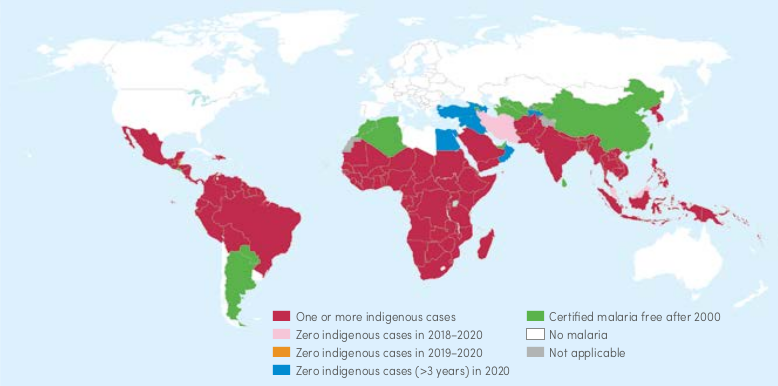
\includegraphics[width=0.9\linewidth]{figure/map_global_malaria_countries} 

}

\caption[Pays d'endémicité palustre en 2000 et leur statut en 2020]{Pays d'endémicité palustre en 2000 et leur statut en 2020 (\protect\hyperlink{ref-who_2021}{WHO, 2021})}\label{fig:map-global-malaria-countries}
\end{figure}
Le poids du paludisme dans le monde est inégalement réparti, à la fois géographiquement et démographiquement. Ainsi par exemple, en 2020, 95~\% des cas et 96~\% de la mortalité étaient concentrés en Afrique sub-saharienne ; et les enfants de moins de 5 ans, tranche de la population la plus vulnérable, représentaient 77~\% de la mortalité (\protect\hyperlink{ref-who_2021}{WHO, 2021}).\\

La morbidité et mortalité liées au paludisme au cours de ces vingt dernières années en Afrique et dans le monde a connu trois phases (figure \ref{fig:malaria-african-trends}). La période 2000 - 2015 a été marquée par une réduction forte et continue de la maladie. L'incidence du paludisme a diminué de 27 \% sur cette période, et la mortalité de 52 \%. Entre 2015 et 2019, les progrès ont stagné. Sur cette période, l'incidence n'a diminué que de 2~\% entre 2015 et 2019 et la mortalité de 16 \%. Enfin, l'année 2020 a été marquée par une augmentation significative des cas et de la mortalité, en partie liés à la pandémie de covid-19 qui a perturbé les services sanitaires (\protect\hyperlink{ref-who_2021}{WHO, 2021}).\\
\begin{figure}

{\centering 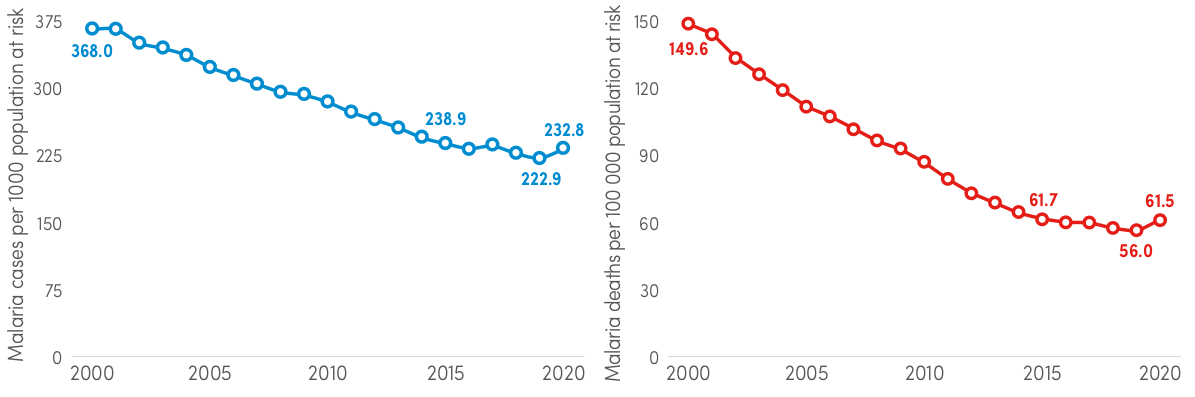
\includegraphics[width=1\linewidth]{figure/malaria_africa_trends} 

}

\caption[Morbité et mortalité annuelle liées au paludisme dans la région Afrique de l'OMS entre 2000 et 2020]{Morbité (à gauche) et mortalité (à droite) annuelle liées au paludisme dans la région Afrique de l'OMS entre 2000 et 2020 (\protect\hyperlink{ref-who_2021}{WHO, 2021})}\label{fig:malaria-african-trends}
\end{figure}
\hypertarget{lagent-pathoguxe8ne-plasmodium}{%
\subsection{\texorpdfstring{L'agent pathogène : \emph{Plasmodium}}{L'agent pathogène : Plasmodium}}\label{lagent-pathoguxe8ne-plasmodium}}

Le paludisme humain est une maladie infectieuse à transmission vectorielle faisant intervenir trois protagonistes : l'homme\footnote{dans ce manuscrit, nous employons le terme ``homme'' pour désigner l'être humain en général, selon la définition du dictionnaire Le Robert} (dit hôte) est infecté par un protozoaire parasite (dit agent infectieux) du genre \emph{Plasmodium} qui lui a été transmis par un moustique (dit vecteur) du genre \emph{Anopheles}. Les rôles de \emph{Plasmodium} et \emph{Anopheles} dans la maladie ont été découverts respectivement en 1880 et 1898 (\protect\hyperlink{ref-cox_history_2010}{Cox, 2010}). Dans les prochaines sections, nous résumons le cycle biologique du parasite et du vecteur, et apportons quelques précisions supplémentaires, d'importance pour la thèse, sur les vecteurs.\\

\hypertarget{diversituxe9-et-distribution}{%
\subsubsection{Diversité et distribution}\label{diversituxe9-et-distribution}}

Parmi les 156 espèces de \emph{Plasmodium} décrites, six causent le paludisme chez l'humain : \emph{Plasmodium falciparum}, \emph{Plasmodium vivax}, \emph{Plasmodium ovale}, \emph{Plasmodium malariae}, \emph{Plasmodium knowlesi} et \emph{Plasmodium cynomolgi}. La plus pathogène des six espèces, \emph{P. falciparum}, est à l'origine de la très grande majorité des cas de paludisme enregistrés en Afrique (\protect\hyperlink{ref-who_2021}{WHO, 2021}) (figure \ref{fig:global-pfpr-2019}). Hors Afrique, c'est \emph{P. vivax} qui prédomine (\protect\hyperlink{ref-who_2021}{WHO, 2021}).\\
\begin{figure}

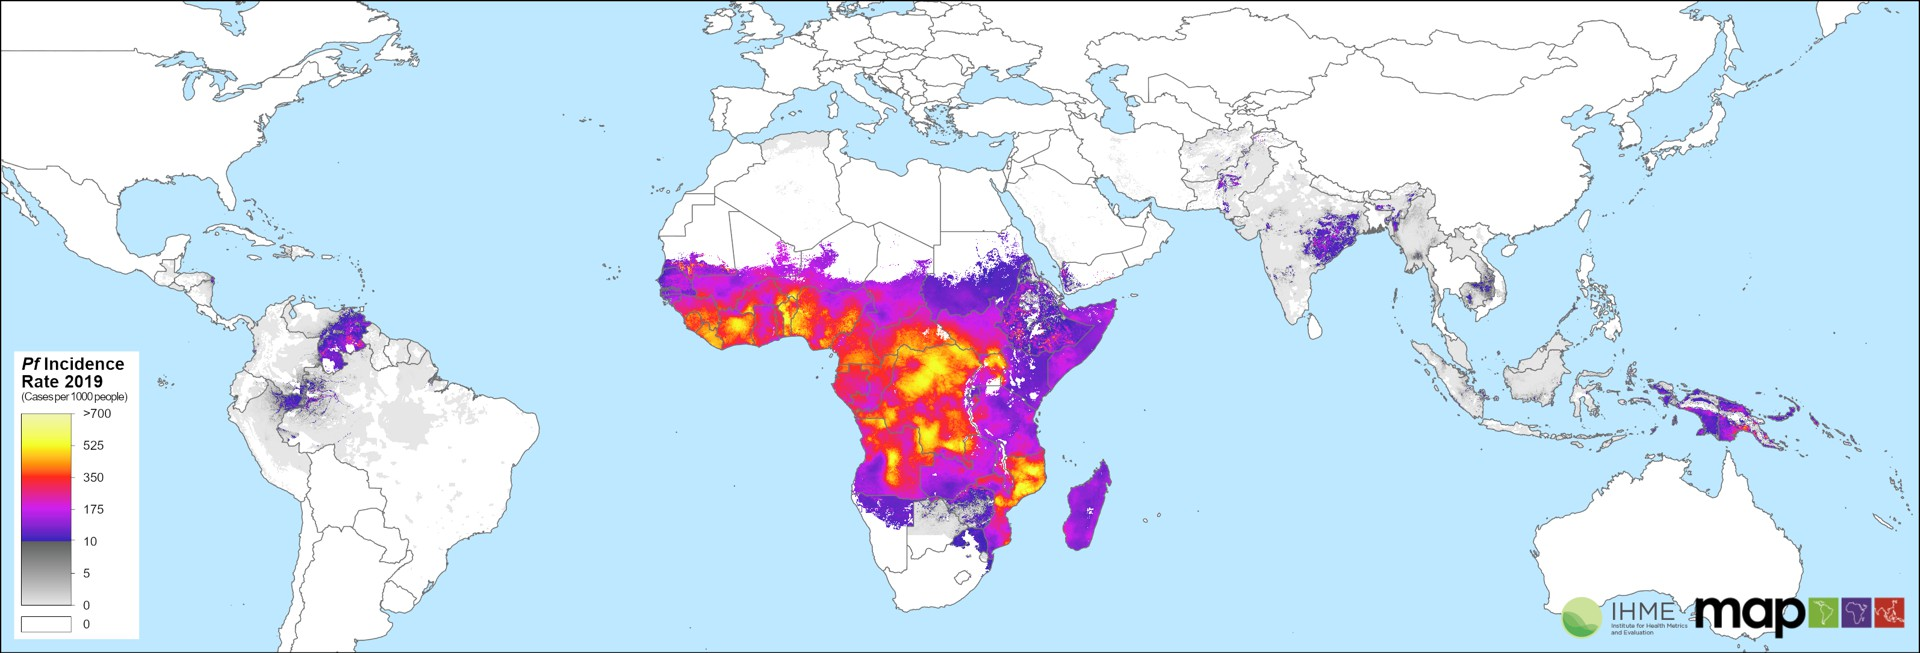
\includegraphics[width=1.1\linewidth]{figure/global_incidence_rate_2019} \hfill{}

\caption[Taux d'incidence du paludisme à Plasmodium falciparum en 2019]{Taux d'incidence du paludisme à Plasmodium falciparum en 2019 (\protect\hyperlink{ref-weiss_mapping_2019}{Weiss et al., 2019})}\label{fig:global-pfpr-2019}
\end{figure}
\hypertarget{cycle-biologique}{%
\subsubsection{Cycle biologique}\label{cycle-biologique}}

Le cycle biologique de \emph{Plasmodium} fait intervenir deux hôtes : un moustique femelle du genre \emph{Anopheles} et un être humain (figure \ref{fig:cycle-tr-palu}). Le cycle chez l'anophèle commence lorsque celui-ci prend un repas sanguin sur un humain infecté, porteur de gamétocytes. Le parasite entame alors dans l'estomac de l'anophèle une phase de multiplication sexuée aboutissant à la migration des sporozoïtes jusqu'aux glandes salivaires du moustique. Ce premier cycle, chez l'anophèle, est appelé cycle sporogonique (ou extrinsèque) et dure environ une dizaine de jours selon l'espèce plasmodiale et la température (\protect\hyperlink{ref-15172}{Baudon, Molez, \& Guiguemde, 1984}). Lors d'une prochaine piqûre une fois le cycle sporogonique effectué, l'anophèle alors infectieux injecte les sporozoïtes à l'homme. Ces derniers migrent dans le foie pour s'y multiplier (phase exo-érythrocytaire, 8 à 10 jours), puis sont libérés dans le sang sous forme de mérozoïtes qui pénètrent dans les globules rouges. S'ensuit une phase de multiplication des mérozoïtes dans les hématies, produisant de nouvelles cellules qui sont à leur tour libérées dans le sang et qui infecteront des érythrocytes sains (phase érythrocytaire). C'est cette libération qui entraîne les symptômes caractéristiques des accès palustres (frissons, chaleur et sueurs). Une partie des parasites peut également subir un processus de différenciation, aboutissant à la formation de gamétocytes mâles et femelles. Lors d'un repas de sang sur l'homme dès lors infectieux, un moustique anophèle femelle peut ingérers ces gamétocytes : le cyle recommence alors.\\
\begin{figure}

{\centering 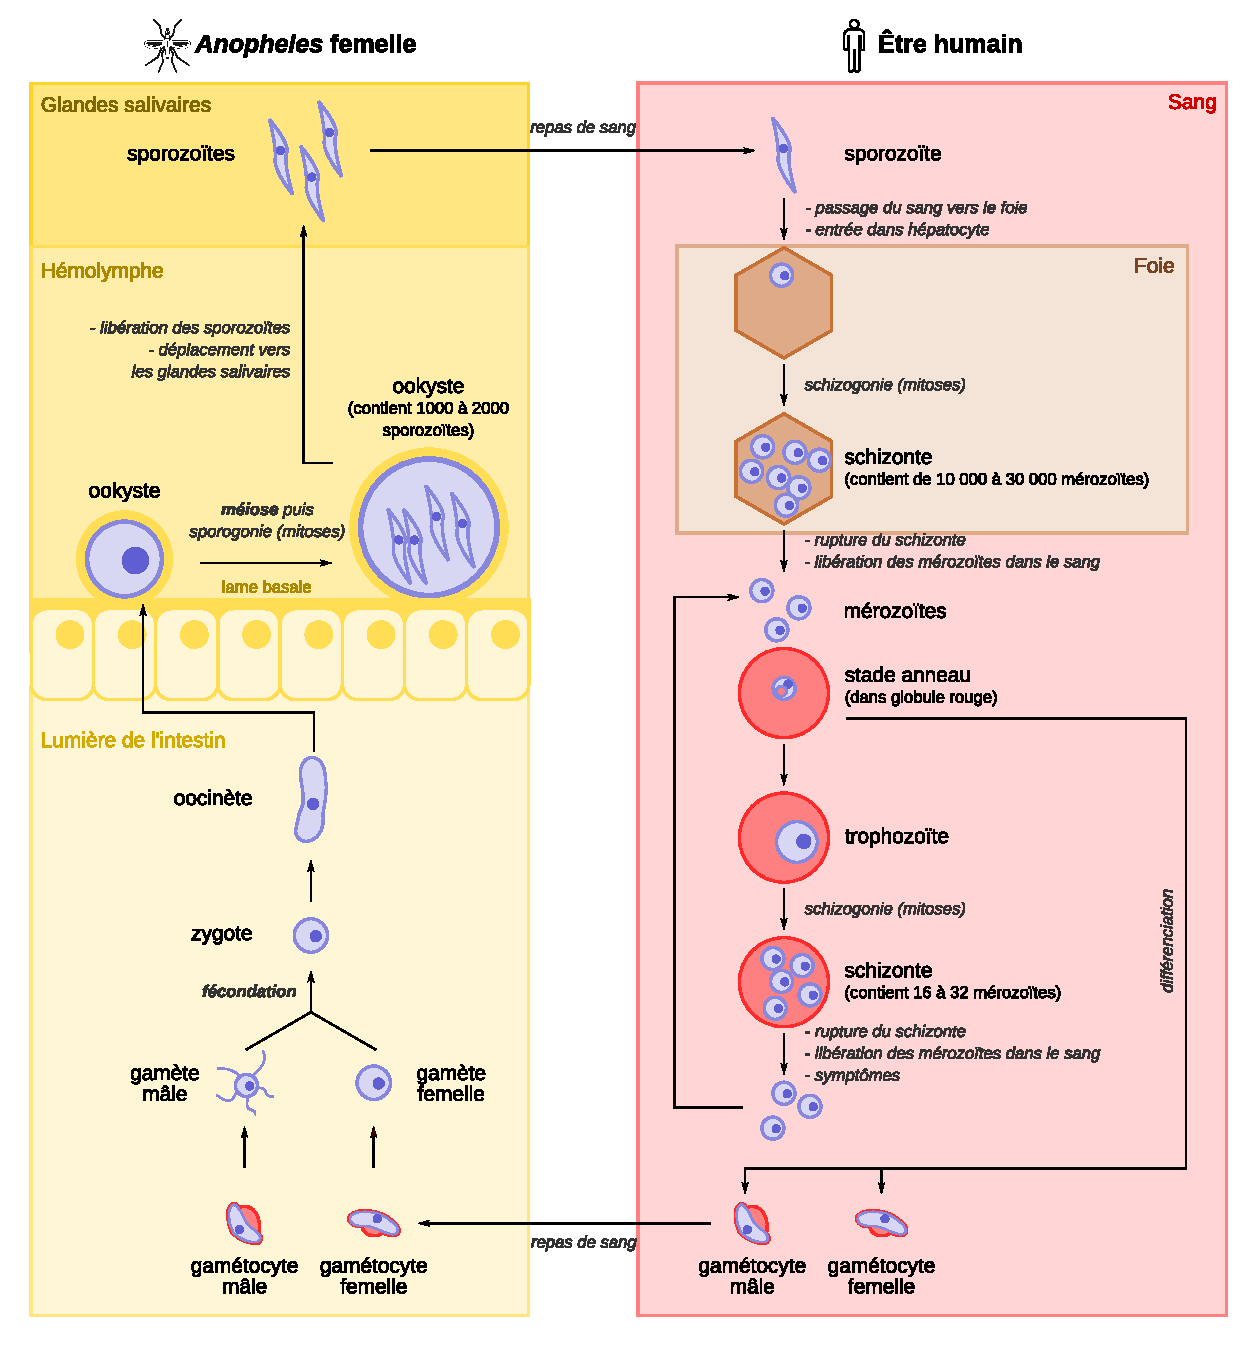
\includegraphics[width=0.8\linewidth]{figure/cycle_transmission_palu_v2} 

}

\caption[Cycle de développement et de reproduction des Plasmodium spp.]{Cycle de développement et de reproduction des Plasmodium spp. (auteur : Pascal Combemorel, License : \href{https://creativecommons.org/licenses/by-sa/4.0/}{CC-BY-SA})}\label{fig:cycle-tr-palu}
\end{figure}
\hypertarget{le-vecteur-anopheles}{%
\subsection{\texorpdfstring{Le vecteur : \emph{Anopheles}}{Le vecteur : Anopheles}}\label{le-vecteur-anopheles}}

\hypertarget{diversituxe9-et-distribution-1}{%
\subsubsection{Diversité et distribution}\label{diversituxe9-et-distribution-1}}

Sur les plus de 3000 espèces de moustiques (\emph{Diptera : Culicidae}) recensées à ce jour, environ 500 font partie du genre \emph{Anopheles}, dont une soixantaine est effectivement vectrice de la maladie. En Afrique sub-saharienne, on trouve au total environ 150 espèces d'anophèles, dont une trentaine vectrice de \emph{Plasmodium}. Dans cette région, les principales espèces vectrices sont \emph{An. arabiensis}, \emph{An. gambiae s.s.} et \emph{An. coluzzii} du complexe Gambiae, et \emph{An. funestus} du groupe Funestus (\protect\hyperlink{ref-sinka_dominant_2010}{Sinka et al., 2010}, \protect\hyperlink{ref-sinka_global_2012}{2012}) (figure \ref{fig:distrib-vectors}).\\
\begin{figure}

{\centering 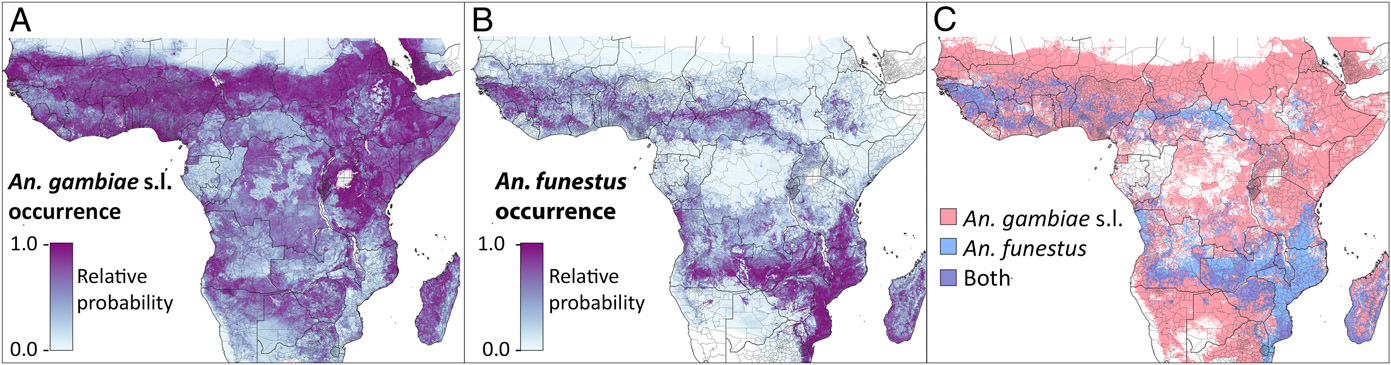
\includegraphics[width=1\linewidth]{figure/distrib_vectors} 

}

\caption[Distribution spatiale d'An. gambiae s.l. et An. funestus en Afrique sub-saharienne]{Distribution spatiale d'An. gambiae s.l. et An. funestus en Afrique sub-saharienne (\protect\hyperlink{ref-moyes_evaluating_2020}{Moyes et al., 2020})}\label{fig:distrib-vectors}
\end{figure}
\hypertarget{cycle-biologique-1}{%
\subsubsection{Cycle biologique}\label{cycle-biologique-1}}

Le cycle biologique de l'anophèle (figure \ref{fig:cycle-biologique-anophele}) comprend quatre stades : oeuf, larve, nymphe et âge adulte. Le stade larvaire (œuf, larve, nymphe) se déroule en milieu aquatique et dure de 1 à 3 semaines en fonction de l'espèce et de la température~; quant au stade adulte, il se déroule en milieu aérien et la durée de vie de l'anophèle femelle peut aller jusqu'à 4 semaines (\protect\hyperlink{ref-holstein_biologie_1952}{Holstein, 1952}). Le stade adulte est marqué par une phase d'accouplement qui a lieu dans les 24 à 48 h suivant l'émergence. L'anophèle femelle ne copule en principe qu'une seule fois et stocke les spermatozoïdes dans une spermathèque jusqu'à sa mort. Une fois accouplée, l'anophèle femelle part à la recherche d'un hôte afin de prendre un repas de sang essentiel à la maturation des follicules ovariens. La piqûre est suivie d'une phase de repos au cours de laquelle la femelle digère le sang. Enfin, la femelle gravide cherche un site d'oviposition et y pond entre 40 et 100 œufs à la surface de l'eau. Après la ponte, la femelle cherche à prendre un nouveau repas sanguin afin d'effectuer une nouvelle oviposition ; et reproduit ce cycle (recherche de repas de sang, piqûre, repos, ponte) jusqu'à sa mort. Ce cycle est appelé gonotrophique et dure 2 à 5 jours en fonction, en particulier, de la température et de l'espèce (\protect\hyperlink{ref-gillies_duration_1953}{Gillies, 1953}; \protect\hyperlink{ref-shapiro_quantifying_2017}{Shapiro, Whitehead, \& Thomas, 2017}; \protect\hyperlink{ref-tchuinkam_bionomics_2010}{Tchuinkam et al., 2010}).\\
\begin{figure}

{\centering 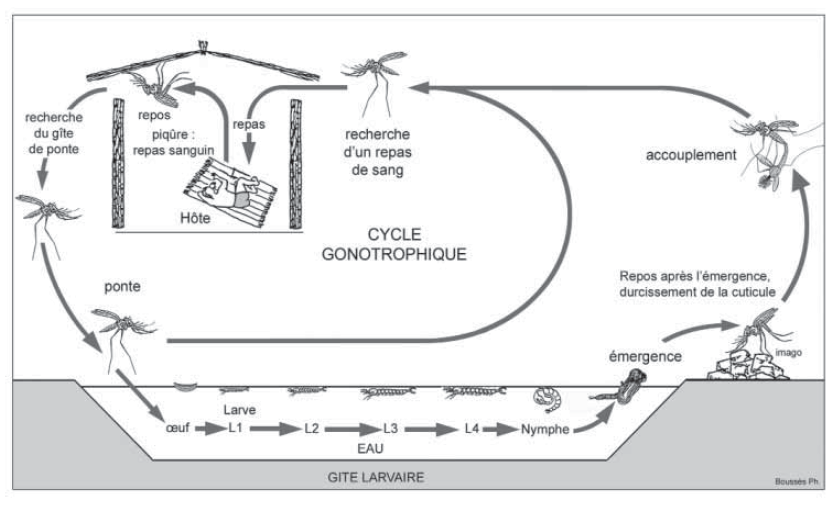
\includegraphics[width=1\linewidth]{figure/carnevale} 

}

\caption[Cycle biologique de l'anophèle]{Cycle biologique de l'anophèle (\protect\hyperlink{ref-carnevale_les_2009}{Carnevale et al., 2009})}\label{fig:cycle-biologique-anophele}
\end{figure}
\hypertarget{comportement-dalimentation}{%
\subsubsection{Comportement d'alimentation}\label{comportement-dalimentation}}

La transmission de \emph{Plasmodium} entre l'anophèle et l'homme s'effectue donc lorsque le vecteur prend un repas de sang sur l'hôte \emph{via} la piqûre. Le comportement de piqûre (dit comportement trophique) de l'anophèle ainsi que son comportement de repos suivant la piqûre sont primordiaux dans l'étude de la transmission du paludisme. Quatre paramètres du comportement trophique et de repos des anophèles sont particulièrement déterminants :
\begin{itemize}
\tightlist
\item
  l'\emph{anthropophilie} : propension d'un vecteur à piquer les humains (à l'opposé de zoophilie, désignant la propension à piquer les animaux) ;
\item
  l'\emph{endophagie} : propension d'un vecteur à piquer à l'intérieur des maisons (à l'opposé d'exophagie, désignant la propension à piquer à l'extérieur des habitations) ;
\item
  l'\emph{endophilie} : propension d'un vecteur à se reposer, après la piqûre, à l'intérieur des maisons (à l'opposé d'exophilie, désignant la propension à se reposer à l'extérieur des habitations) ;
\item
  l'\emph{activité précoce ou tardive} : propension d'un vecteur à piquer précocément ou tardivement dans la nuit, par rapport aux horaires habituellement observés (voir ci-dessous).\\
\end{itemize}
\hypertarget{elements-de-bionomie}{%
\subsubsection{Elements de bionomie}\label{elements-de-bionomie}}

Bien que le cycle biologique de tous les anophèles soit identique, les différentes espèces (ainsi que les différents individus au sein d'une même espèce) exhibent souvent des préférences écologiques ou trophiques sensiblement différentes. Ci-après, nous donnons quelques éléments de bionomie (gites larvaires et comportements préférentiels) des 4 principales espèces d'anophèles vectrices en Afrique sub-saharienne. Ces éléments sont intégralement extraits de synthèses bibliographiques sur la bionomie des vecteurs effectuées à l'échelle de l'Afrique sub-saharienne, effectuées par Sinka et al. (\protect\hyperlink{ref-sinka_dominant_2010}{2010}) (gites larvaires préférentiels + comportements trophiques) et Sherrard-Smith et al. (\protect\hyperlink{ref-sherrard-smith_mosquito_2019}{2019}) (comportement trophique).\\

\emph{An. gambiae s.s.} et \emph{An coluzzii} sont des espèces majoritairement associées aux gites larvaires respectivement temporaires et semi-permanents, globalement d'eaux douces peu profondes et ensoleillées. Ainsi, les larves d'\emph{An. gambiae s.s.} sont typiquement retrouvées dans les gites se remplissant avec les précipitations, telles que les flaques d'eau, les empreintes de sabot ou les ornières ; et \emph{An. coluzzii} pond typiquement dans les rizières ou zones inondées contenant de la végétation flottante et immergée, telles que les bas-fonds et zones marécageuses. Les deux espèces ont été décrites comme hautement anthropophiles et majoritairement endophages et endophiles. L'activité de piqûre de ces espèces se concentre au milieu de la nuit avec une tendance à la piqûre plutot tardive (figure \ref{fig:courbes-agressivite-anopheles}). Malgré ces grandes tendances, ces espèces présentent une certaine plasticité phénotypique dans leur comportement de piqûre et de repos.\\
\begin{figure}

{\centering 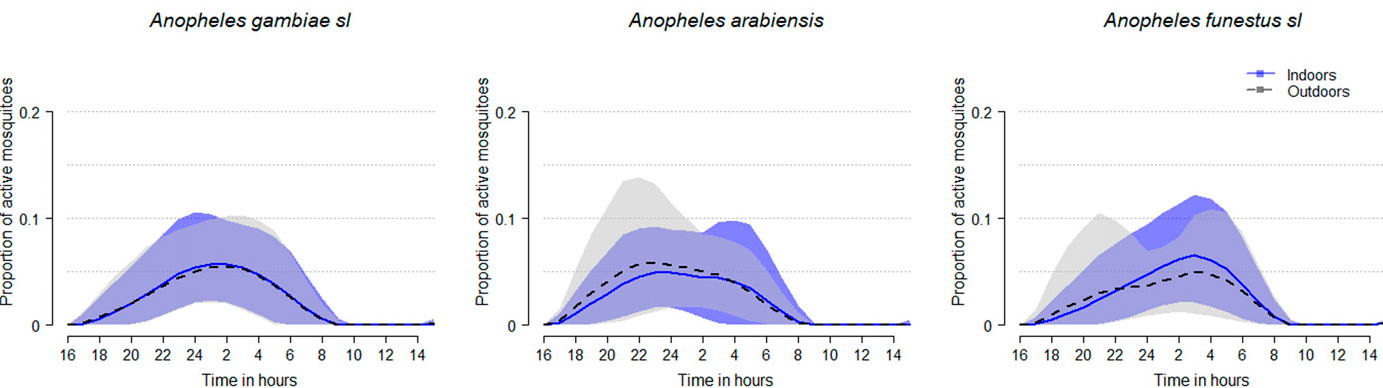
\includegraphics[width=1\linewidth]{figure/courbes_agressivite_vecteurs} 

}

\caption[Courbes d’agressivité horaire nocturne pour trois espèces majeures d'anophèles en Afrique]{Courbes d’agressivité horaire nocturne pour trois espèces majeures d'anophèles en Afrique (\protect\hyperlink{ref-sherrard-smith_mosquito_2019}{Sherrard-Smith et al., 2019})}\label{fig:courbes-agressivite-anopheles}
\end{figure}
\emph{An. arabiensis} est une espèce associée aux environnements de savanes et forêts clairsemées. Les gites larvaires d'\emph{An. arabiensis} ressemblent à ceux d'\emph{An. gambiae s.s.} : petits bassins d'eau douce temporaires, ensoleillés, clairs et peu profonds ; bien que l'espèce ait également été observée dans d'autres gites larvaires plus profonds ou turbides. \emph{An. arabiensis} est considérée davantage zoophage, exophage et exophile qu'\emph{An. gambiae s.s.}. Cependant, l'espèce montre un large éventail de comportements de piqûre et de repos en fonction des zones géographiques, constituant ainsi une espèce au comportement a piori plus plastique encore qu'\emph{An. gambiae}. \emph{An. arabiensis} pique en moyenne plus tôt dans la nuit qu'\emph{An. gambiae}. Les courbes d'agressivité diffèrent cependant selon le site de piqûre, les vecteurs exophages étant actifs relativement plutôt précocément et les vecteurs endophages relativement plus tardivement (figure \ref{fig:courbes-agressivite-anopheles}).\\

\emph{An. funestus}, de son côté, est une espèce majoritairement associée aux grandes étendues d'eau douces, permanentes ou semi-permanentes, contenant une végétation émergente ou flottante, comme les marécages, les grands étangs et les bords de lacs. C'est une espèce décrite comme hautement adaptable, ce qui lui permet d'occuper et de maintenir une distribution spatiale large. \emph{An. funestus} est considérée hautement anthropophile. L'espèce est majoritairement endophage, et présente un comportement de piqûre relativement tardif (figure \ref{fig:courbes-agressivite-anopheles}). Par rapport aux autres espèces de vecteurs dominantes en Afrique, \emph{An. funestus} présente des schémas comportementaux assez stables (généralement anthropophile et endophile) dans l'ensemble de son aire de répartition.\\

\hypertarget{le-systuxe8me-vectoriel}{%
\subsection{Le système vectoriel}\label{le-systuxe8me-vectoriel}}

Pour que la transmission du paludisme puisse s'effectuer, hôte, vecteur et agent infectieux doivent interagir dans un environnement favorable (\protect\hyperlink{ref-reisen_landscape_2010}{Reisen, 2010}). La triade vectorielle (système composé de l'agent pathogène, du vecteur et de l'hôte), complétée de l'environnement dans lequel elle évolue et de l'ensemble des interactions entre les acteurs et l'environnement, forme le \emph{système vectoriel} (\protect\hyperlink{ref-rodhain_microbe_2015}{Rodhain, 2015}) (figure \ref{fig:systeme-vectoriel}). Comme nous allons le voir plus loin (section \ref{enjeux-objectifs-these}), l'analyse des intéractions dans le système vectoriel est au cœur de l'étude du risque de transmission du paludisme, et plus largement des maladies à transmission vectorielle.
\begin{figure}

{\centering 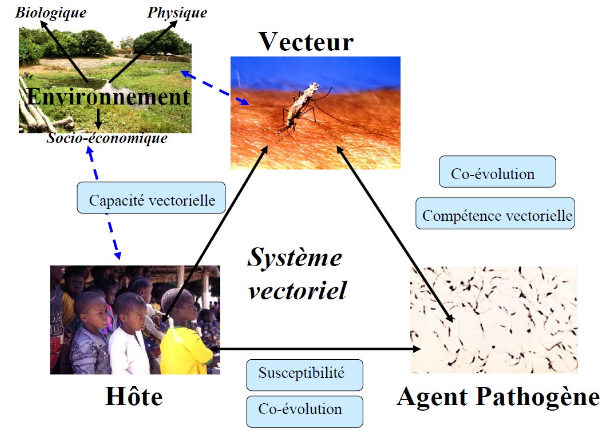
\includegraphics[width=0.7\linewidth]{figure/systeme_vectoriel} 

}

\caption[Le sytème vectoriel]{Système vectoriel : agent pathogène, vecteur, hôte, environnement (\protect\hyperlink{ref-fontenille_2019}{Fontenille, 2009})}\label{fig:systeme-vectoriel}
\end{figure}
De part son impact sur les traits de vie de chacun des protagonistes de la triade vectorielle, l'environnement (pris au sens large du terme : météorologie, paysage, facteurs socio-culturels, etc.) conditionne considérablement les dynamiques épidémiologiques, notamment spatio-temporelles, des maladies vectorielles (\protect\hyperlink{ref-reisen_landscape_2010}{Reisen, 2010}). Ainsi par exemple, des traits de vie des anophèles tels que l'émergence, la croissance, la survie, la dispersion, ou encore l'activité (notamment trophique) peuvent être impactés par des facteurs environnementaux météorologiques (températures, précipitations, humidité, etc.), paysagers (utilisation et occupation du sol, etc.), anthropiques (interventions de lutte contre les vecteurs, etc.), etc.\footnote{Les liens entre environnement et traits de vie des anophèles sont plus largement détaillés dans les chapitres 4 et 5 du manuscrit}. Il en découle que certains indicateurs entomologiques de la transmission tels que la densité agressive des vecteurs (nombre de piqûres / homme / nuit) sont, à priori, largement dépendants des conditions environnementales (\protect\hyperlink{ref-moiroux_modelling_2013}{Moiroux et al., 2013}, \protect\hyperlink{ref-moiroux_spatio-temporal_2014}{2014}). La figure \ref{fig:complex-system-anopheles} expose par exemple un ensemble de facteurs ayant été identifiés, dans la bibliographie, comme pouvant impacter les densités agressives des anophèles (`m.a. vecteur'), ainsi que les relations à priori existantes entre ces facteurs (\protect\hyperlink{ref-moiro2012}{Moiroux, 2012}).
\begin{figure}

{\centering 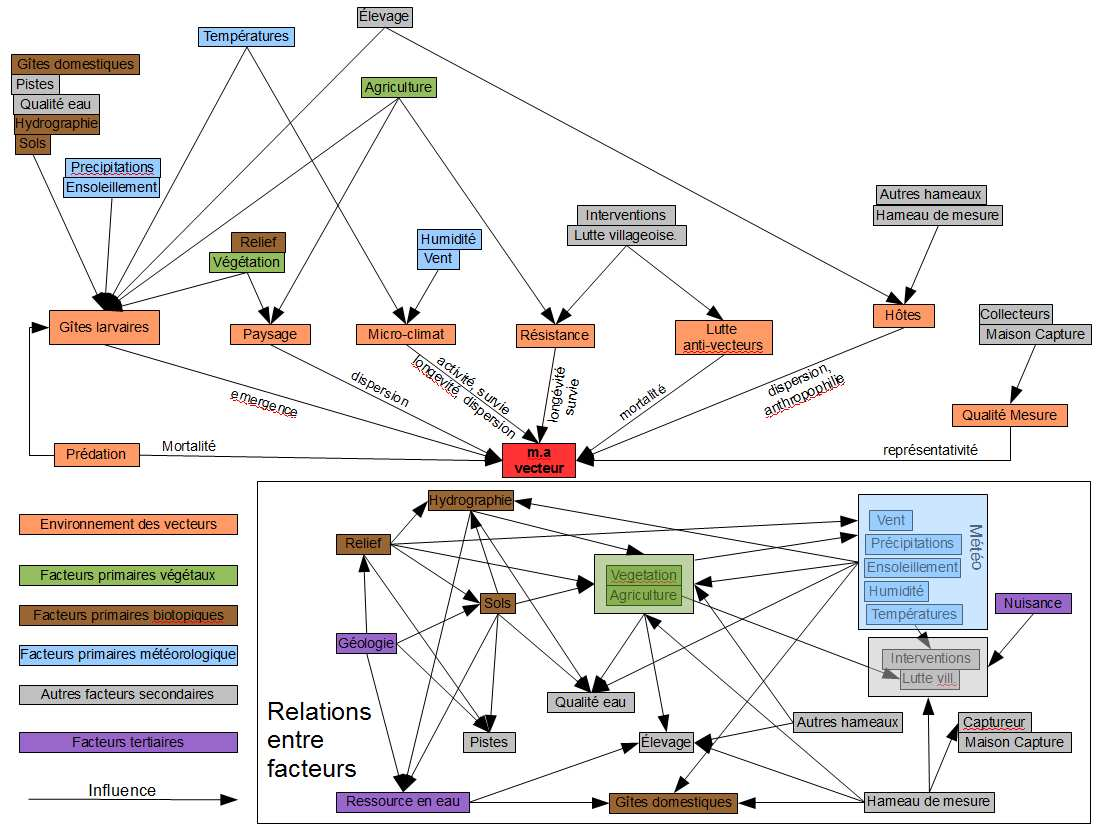
\includegraphics[width=1\linewidth]{figure/systeme_complexe_abondance_vecteurs} 

}

\caption[Modèle conceptuel du système \{densités agressives des anophèles - environnement\}]{Modèle conceptuel du système biologique \{densités agressives des anophèles - environnement\} (\protect\hyperlink{ref-moiro2012}{Moiroux, 2012})}\label{fig:complex-system-anopheles}
\end{figure}
\hypertarget{lutte-anti-vectorielle}{%
\subsection{Lutte anti-vectorielle}\label{lutte-anti-vectorielle}}

La lutte contre le paludisme s'oriente autour de trois axes : i) prévention, ii) diagnostic des cas suspects et iii) traitement des cas confirmés. Le diagnostic et le traitement visent respectivement à identifier la présence de \emph{Plasmodium} dans le corps humain et à traiter les cas confirmés. La prévention, en amont, vise à réduire le risque de transmission ou les conséquences de la maladie si l'infection a lieu. Trois méthodes de prévention existent : la chimiothérapie préventive, la vaccination, et la lutte anti-vectorielle (\protect\hyperlink{ref-who_2021}{WHO, 2021}). Attardons-nous sur la lutte anti-vectorielle, seule des trois méthodes ciblant le moustique vecteur.\\

\hypertarget{concept}{%
\subsubsection{Concept}\label{concept}}

La lutte anti-vectorielle (LAV) consiste en un ensemble d'outils et de méthodes visant à empêcher la transmission des parasites depuis le vecteur vers l'humain. Dans leur immense majorité, ces outils ont pour objectif de limiter la probabilité (i) soit qu'un contact entre l'anophèle et l'humain se réalise (cad. la piqûre, ou encore l'intéraction homme-vecteur), (ii) soit qu'un moustique atteigne l'âge épidémiologiquement dangereux, (iii) soit les deux. Les leviers d'action sont multiples : réduire la densité des vecteurs, réduire leur longévité, ou empêcher physiquement le contact homme-vecteur. Pour cela, toutes sortes d'outils de lutte anti-vectorielle existent.

\hypertarget{lav-principaux-outils}{%
\subsubsection{Principaux outils de LAV}\label{lav-principaux-outils}}

Comme présenté précédemment, les principaux vecteurs du paludisme en Afrique ont été historiquement décrits comme majoritairement endophages, endophiles et nocturnes. C'est sur la base de ces traits comportementaux qu'ont été élaborés les deux principaux outils de lutte anti-vectorielle utilisés aujourd'hui dans la lutte contre la paludisme (\protect\hyperlink{ref-who_2021}{WHO, 2021}) : la moustiquaire Imprégnée d'Insecticide à Longue Durée d'Action (MIILDA) et les Pulvérisations Intra-Domiciliaires d'insecticide à effet rémanent (PID).\\

La MIILDA est un rideau de tulle imprégné d'insecticide dont on entoure en général les lits. La MIILDA offre une double barrière face aux vecteurs :
\begin{itemize}
\tightlist
\item
  barrière physique : le rideau de tulle offre une protection individuelle contre les vecteurs pour les personnes utilisant la moustiquaire, en empêchant le vecteur en recherche de repas de sang d'entrer en contact avec l'hôte
\item
  barrière chimique : l'insecticide dont la MIILDA est imprégnée a un effet à la fois repulsif (à distance) et létal (pour les vecteurs entrant en contact avec la moustiquaire).
\end{itemize}
Cette barrière chimique réduit donc la longévité des vecteurs sensibles à l'insecticide, et ainsi sa probabilité d'atteindre l'âge epidémiologiquement dangereux. Par ailleurs, en réduisant la longévité des vecteurs individuellement, les MIILDA réduisent leur densité de population globale, et protègent donc théoriquement également les non-utilisateurs de moustiquaires dans la communauté (\protect\hyperlink{ref-hawley_community-wide_2003}{Hawley et al., 2003}; \protect\hyperlink{ref-killeen_exploring_2007}{Gerry F. Killeen \& Smith, 2007}). Cet effet de protection, appelé ``communautaire'', se manifeste au delà d'un certain seuil d'utilisation des MIILDA dans une communauté donnée (les exercices de modélisation mathématique avancent un seuil situé entre 35 \% et 65 \% en fonction des spécificités écologiques locales (\protect\hyperlink{ref-killeen_preventing_2007}{Gerry F. Killeen et al., 2007})).\\

La MIILDA a été l'outil de LAV phare du programme mondial de lutte contre le paludisme \emph{Roll back malaria}, lancé par l'OMS en 2000. Ainsi, au niveau mondial, 2,3 milliards de moustiquaires imprégnées d'insecticide ont été vendues par les producteurs entre 2004 et et 2020 (\protect\hyperlink{ref-who_2021}{WHO, 2021}) ; et une grande partie de ces moustiquaires a été distribuée aux populations exposées au risque de paludisme par le biais des différents Programmes Nationaux de Lutte contre le Paludisme (PNLP)\footnote{Organismes nationaux chargés de mettre en oeuvre les politiques de lutte contre le paludisme}. On estime en 2020 que 65\% des maisons en Afrique sub-Saharienne étaient équipées d'au moins une moustiquaire et que 43 \% de la population dormait sous une moustiquaire (\protect\hyperlink{ref-who_2021}{WHO, 2021}). L'efficacité des MIILDA a été largement documentée et prouvée~: on estime qu'elle a permis d'éviter environ 450 millions de cas de paludisme et 1 million de décès associés entre 2000 et 2015 (\protect\hyperlink{ref-bhatt_effect_2015}{Bhatt et al., 2015}).\\

Les PID sont, après la MIILDA, le deuxième outil de LAV le plus communément utilisé (\protect\hyperlink{ref-who_2021}{WHO, 2021}). La méthode des PID consiste à pulvériser un insecticide sur les murs intérieurs d'une habitation, afin de réduire la longévité (et donc la densité) des vecteurs venant se reposer sur les murs intérieurs de l'habitation après la piqûre. Elle vise donc les vecteurs endophiles. En 2020, 5,3 \% de la population africaine à risque était protégée par les PID (\protect\hyperlink{ref-who_2021}{WHO, 2021}).\\
\begin{figure}

{\centering 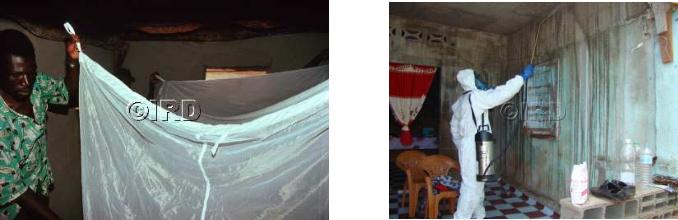
\includegraphics[width=1\linewidth]{figure/milda_pid} 

}

\caption[Installation d'une moustiquaire imprégnée et pulvérisations intra-domiciliaire d'insecticide]{Installation d'une moustiquaire imprégnée (gauche) et pulvérisations intra-domiciliaire d'insecticide (droite) (crédit photo : Jean-Jacques Lemasson et Vincent Robert)}\label{fig:milda-pid}
\end{figure}
Une myriade d'outils et méthodes de lutte anti-vectorielle existent en sus de la MIILDA et des PID (\protect\hyperlink{ref-wilson_importance_2020}{Wilson et al., 2020}) (la figure \ref{fig:vc-tools} en présente certains), mais restent à ce jour utilisés en proportion bien moindre : les répulsifs individuels, la lutte anti-larvaire, les pulvérisations spatiales extérieures, la lutte génétique, les grillages de fenêtres, etc.
\begin{figure}

{\centering 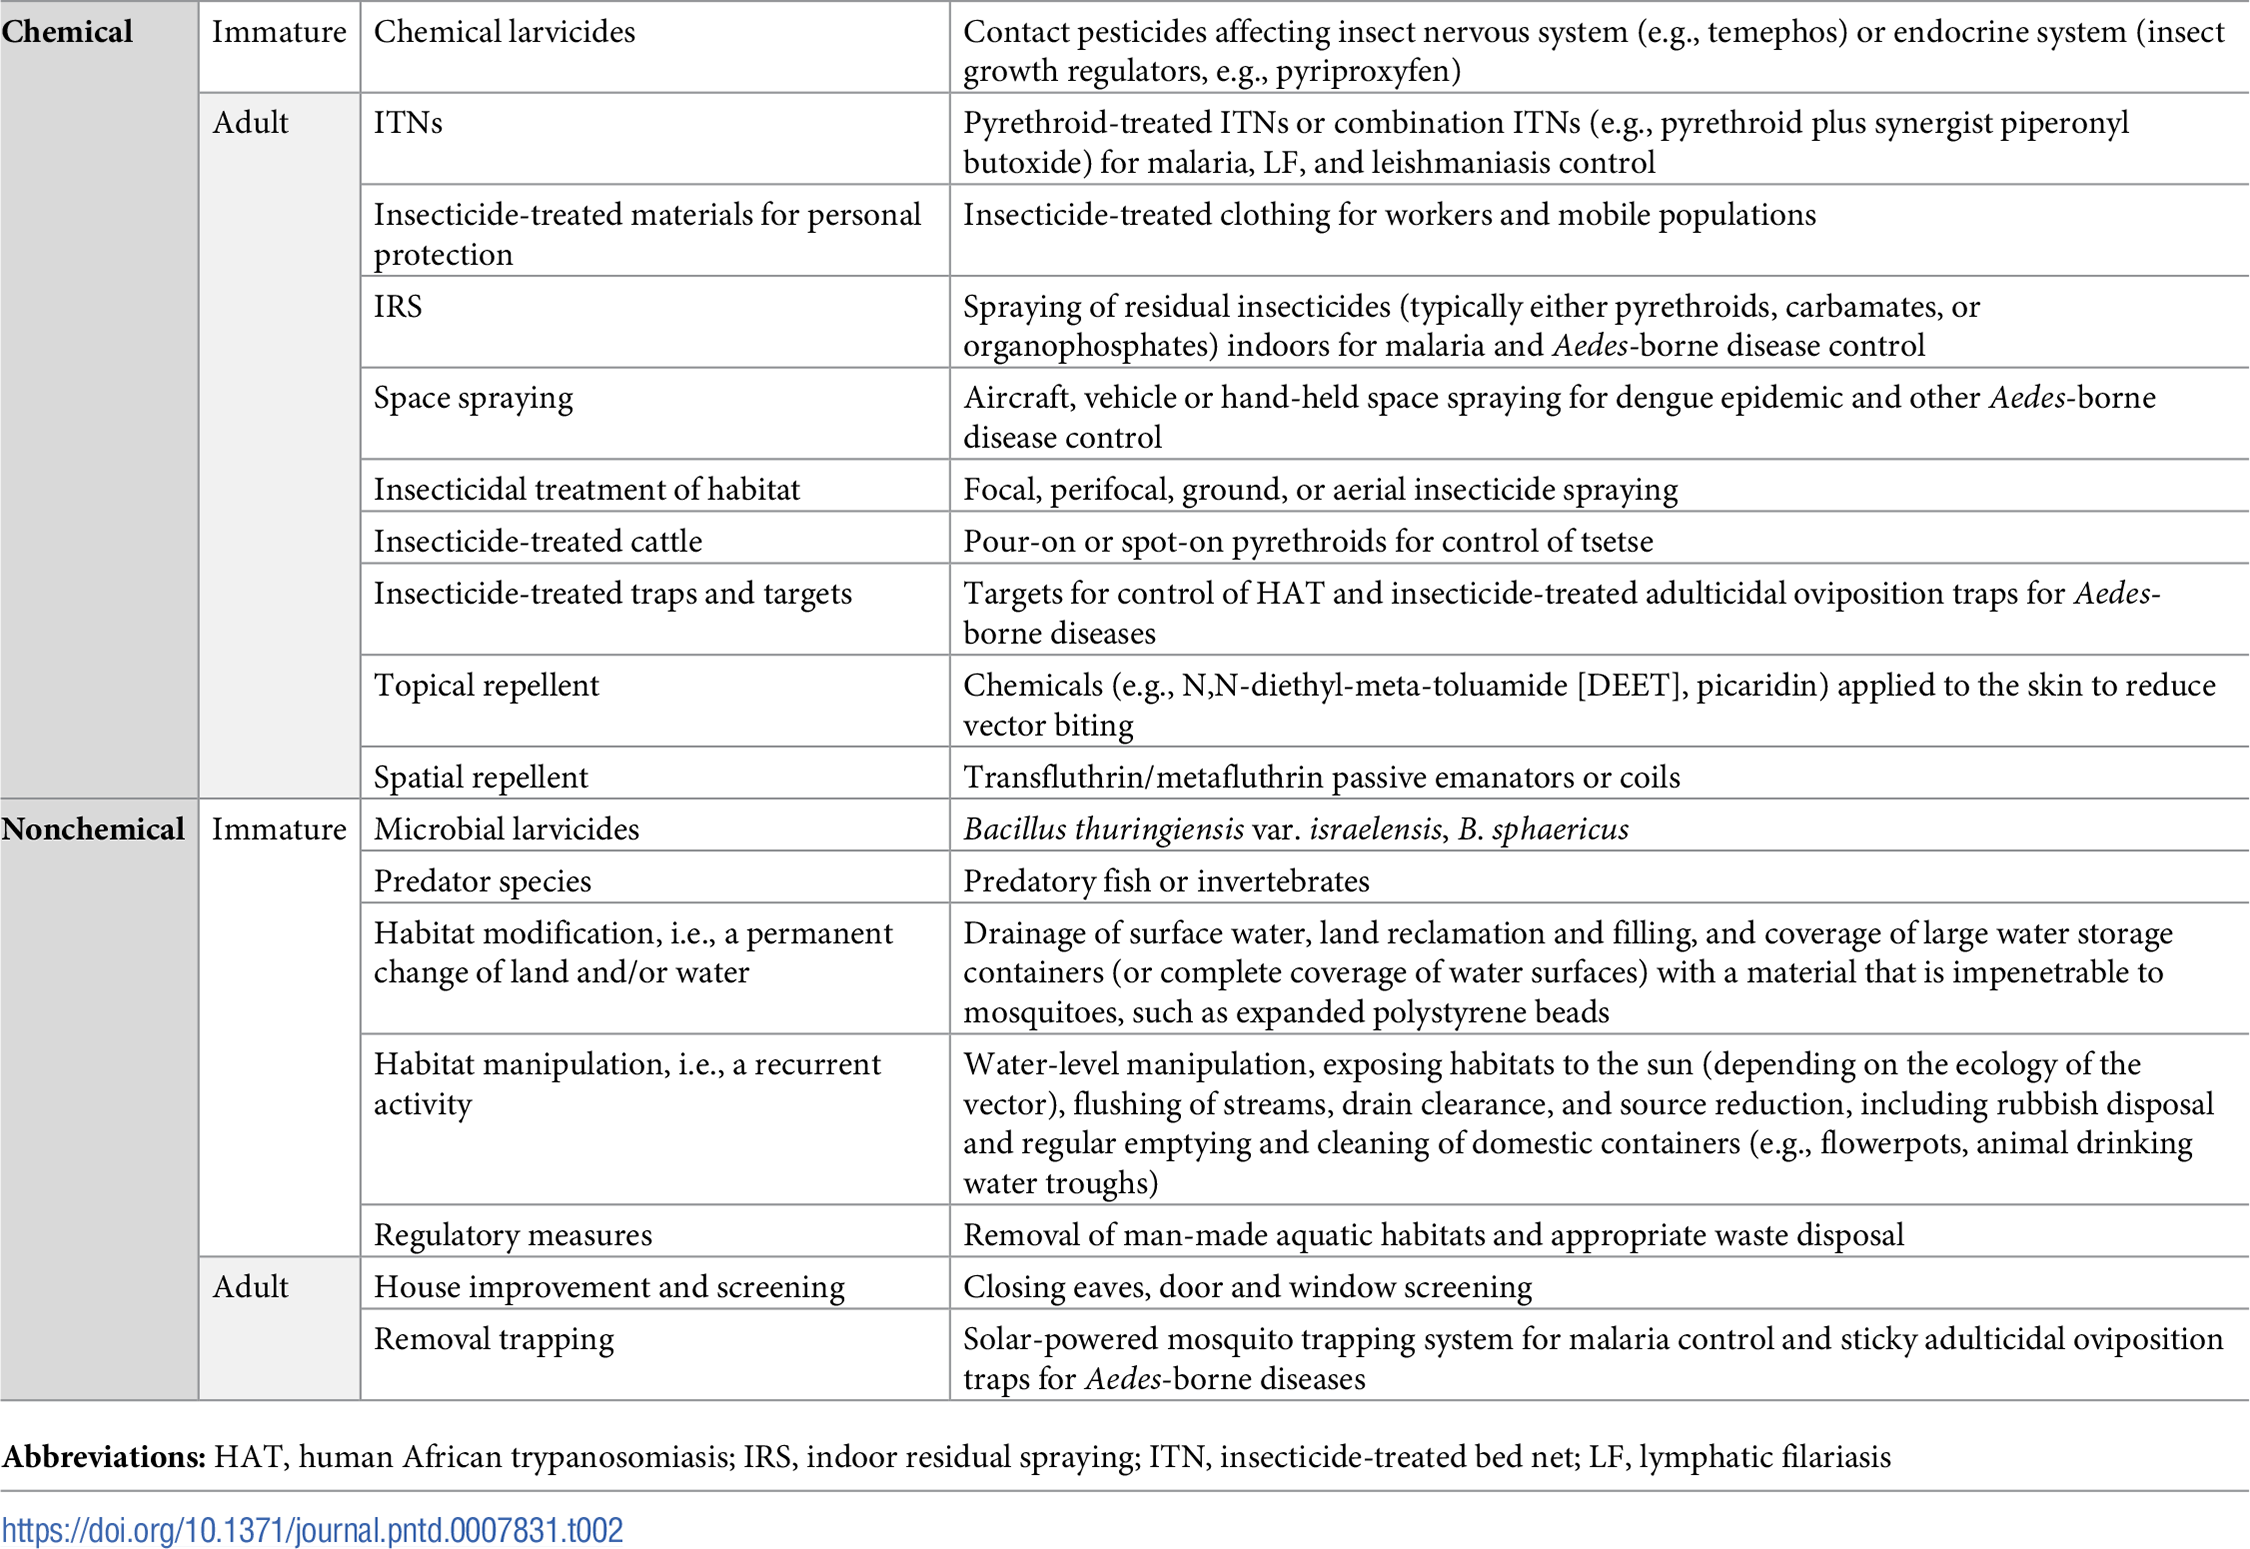
\includegraphics[width=1\linewidth]{figure/vc_tools} 

}

\caption[Exemples d'outils de lutte anti-vectorielle]{Exemples d'outils de LAV utilisés contre la transmission des maladies vectorielles, triés par catégories (basés ou non sur les insecticides) et stade de développement du vecteur ciblé (\protect\hyperlink{ref-wilson_importance_2020}{Wilson et al., 2020})}\label{fig:vc-tools}
\end{figure}
\hypertarget{transmission-ruxe9siduelle-du-paludisme-probluxe9matique-duxe9finition-enjeux}{%
\section{Transmission résiduelle du paludisme : problématique, définition, enjeux}\label{transmission-ruxe9siduelle-du-paludisme-probluxe9matique-duxe9finition-enjeux}}

\hypertarget{limites-actuelles-de-la-lav}{%
\subsection{Limites actuelles de la LAV}\label{limites-actuelles-de-la-lav}}

Ces outils, MIILDA en tête, ont donc été et restent les principaux artisans de la diminution de l'incidence du paludisme à large échelle. Cependant, les niveaux toujours soutenus de transmission et la récente stagnation - voire augmentation dans certaines régions - du nombre de cas de paludisme dans des régions pourtant couvertes par ces outils, questionne : quelles en sont les limites ? Pourquoi cette stagnation ? Plusieurs hypothèses sont généralement avancées :
\begin{itemize}
\item
  \emph{Fraction de la population de vecteurs ciblés.} Ces outils présentent certaines limites intrinsèques. Comme expliqué précédemment, les MIILDA et les PID ciblent, par définition, les vecteurs endophages, endophiles, et anthropophages. Le corollaire à cette observation est que tout vecteur exophage, exophile, ou zoophage leur échappe. Aussi, dans les zones où les vecteurs montrent de tels comportements, ces outils sont à priori peu efficaces (\protect\hyperlink{ref-killeen_characterizing_2014}{Gerry F. Killeen, 2014}).
\item
  \emph{Taux de possession et d'utilisation.} Ces outils ne sont efficaces que s'ils sont disponibles et utilisés. Bien qu'assez triviale, cette assertion peut expliquer en partie les niveaux toujours élevés de transmission. Comme énoncé précedemment, la couverture en outils de LAV et leur utilisation est loin d'être universelle. Par ailleurs, les taux de possession et utilisation de moustiquaires sont très variables selon les sous-régions, pays, et à des échelles spatiales plus fines encore (\protect\hyperlink{ref-bertozzi-villa_maps_2021}{Bertozzi-Villa et al., 2021}) (figure \ref{fig:itn-access-use}). Notons, sur la figure \ref{fig:itn-access-use}, l'évolution de la possession et utilisation des moustiquaires à l'échelle de l'Afrique : les taux moyens ont fortement augmenté entre 2000 et 2017 mais déclinent depuis cette année-ci.
\end{itemize}
\begin{figure}

{\centering 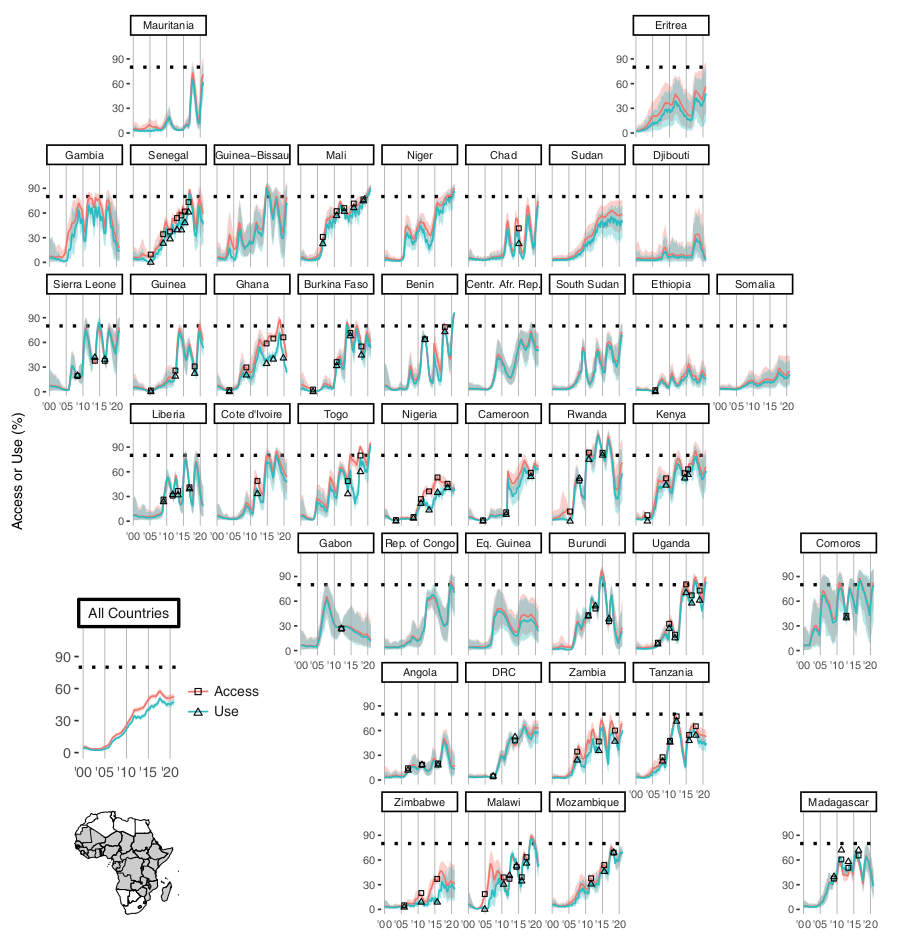
\includegraphics[width=1\linewidth]{figure/itn_access_use2} 

}

\caption[Evolution du taux de possession et d'utilisation de moustiquaires par pays en Afrique]{Evolution du taux de possession et d'utilisation de moustiquaires par pays en Afrique (\protect\hyperlink{ref-bertozzi-villa_maps_2021}{Bertozzi-Villa et al., 2021})}\label{fig:itn-access-use}
\end{figure}
\begin{itemize}
\item
  \emph{Altération de la composition spécifique des vecteurs.} Ces outils sont susceptibles d'altérer la composition spécifique des vecteurs, en réduisant, à terme, la part des vecteurs endophiles, endophages, anthropophages, nocturnes et en favorisant les espèces exophages, exophiles, zoophages, et piquant précocément ou tardivement (\protect\hyperlink{ref-derua_change_2012}{Derua et al., 2012}; \protect\hyperlink{ref-gatton_importance_2013}{Gatton et al., 2013}; \protect\hyperlink{ref-mwangangi_shifts_2013}{Mwangangi et al., 2013}; \protect\hyperlink{ref-russell_increased_2011}{Russell et al., 2011}; \protect\hyperlink{ref-sougoufara_shift_2016}{S. Sougoufara, Harry, Doucouré, Sembène, \& Sokhna, 2016}). Ces vecteurs, non ciblés par les MIILDA ou les PID, seront alors susceptibles de transmettre le paludisme.
\item
  \emph{Développement de mécanismes de résistance aux insecticides.} Enfin, on observe que les vecteurs au départ ciblés par ces outils développent des mécanismes de résistance aux insecticides leur permettant d'éviter ou de contourner leurs effets léthaux (\protect\hyperlink{ref-corbel_distribution_2013}{Corbel \& N'Guessan, 2013}; \protect\hyperlink{ref-manguin_residual_2013}{Durnez \& Coosemans, 2013}; \protect\hyperlink{ref-gatton_importance_2013}{Gatton et al., 2013}; \protect\hyperlink{ref-killeen_characterizing_2014}{Gerry F. Killeen, 2014}; \protect\hyperlink{ref-riveron_insecticide_2018}{Riveron et al., 2018}).
\end{itemize}
Parmi les différentes limites et problématiques sus-mentionnées, le développement de résistances aux insecticides dans les populations vectorielles est particulièrement important et probablement, impactant. En effet, les résistances menacent directement l'efficacité des principaux outils de lutte anti-vectorielle. La section suivante précise les différentes formes de résistance décrites dans la littérature, présente brièvement les mécanismes impliqués dans le développement des résistances, et décrit succinctement leur distribution spatio-temporelle en Afrique.

\hypertarget{ruxe9sistances-des-anophuxe8les-aux-insecticides}{%
\subsection{Résistances des anophèles aux insecticides}\label{ruxe9sistances-des-anophuxe8les-aux-insecticides}}

On reconnaît deux formes principales de résistances des vecteurs aux insecticides : les résistances physiologiques et les résistances comportementales (\protect\hyperlink{ref-lockwood_evolution_1984}{Lockwood, Sparks, \& Story, 1984}; \protect\hyperlink{ref-sokhna_changes_2013}{Sokhna, Ndiath, \& Rogier, 2013}).\\

\hypertarget{ruxe9sistances-physiologiques}{%
\subsubsection{Résistances physiologiques}\label{ruxe9sistances-physiologiques}}

La résistance physiologique fait référence à un ensemble de mécanismes qui permettent au moustique de survivre à un contact avec l'insecticide (\protect\hyperlink{ref-davidson_insecticide_1957}{Davidson, 1957}). Les bases moléculaires et génétiques de la résistance physiologique sont bien connues : sous la pression des insecticides, les mutations qui permettent aux vecteurs de survivre sont naturellement sélectionnées et se propagent ensuite dans les générations successives (\protect\hyperlink{ref-labbe_evolution_2017}{Labbé et al., 2017}; \protect\hyperlink{ref-martinez-torres_molecular_1998}{Martinez-Torres et al., 1998}).\\

Plusieurs mécanismes de résistance physiologique aux insecticides ont été décrits, notamment biochimiques et morphologiques. Les modifications de la cible physiologique de l'insecticide - forme de résistance physiologique qui va être étudiée dans la suite de cette thèse - provoquent une réduction de la sensibilité aux insecticides en raison de mutations ponctuelles sur les gènes codant pour les protéines cibles (\protect\hyperlink{ref-davies_ddt_2007}{Davies, Field, Usherwood, \& Williamson, 2007}; \protect\hyperlink{ref-oreilly_modelling_2006}{O'Reilly et al., 2006}). La mutation la plus commune décrite chez les membres du complexe \emph{Gambiae} est la mutation dite ``kdr'' (``knock-down resistance''). Cette mutation induit une résistance aux pyréthrinoïdes et aux organochlorés, insecticides les plus largement utilisés dans la lutte anti-vectorielle. On distingue 2 formes principales pour cette mutation : la mutation L1014F (ou ``kdr-ouest'') - historiquement détectée et largement répandue en Afrique de l'Ouest - et la mutation L1014S (ou ``kdr-est'') - historiquement détectée et largement répandue en Afrique de l'Est (\protect\hyperlink{ref-martinez-torres_molecular_1998}{Martinez-Torres et al., 1998}; \protect\hyperlink{ref-ranson_identification_2000}{Ranson et al., 2000}). Une autre mutation dite ``ace-1'' (G119S) induit chez les anophèles une résistance aux carbamates, et dans une moindre mesure, aux organochlorés (\protect\hyperlink{ref-weill_unique_2004}{Weill et al., 2004}).\\

Bien que les premières traces de résistances physiologiques chez les anophèles aient été observées bien avant les distributions massives des MIILDA (\protect\hyperlink{ref-corbel_distribution_2013}{Corbel \& N'Guessan, 2013}), on note une corrélation temporelle forte entre le déploiement à large échelle des outils de lutte anti-vectorielle (figure \ref{fig:itn-access-use}) et la généralisation des résistances physiologiques chez les vecteurs du paludisme depuis les années 2000 (figure \ref{fig:dev-res-phy}). La problématique des résistances physiologiques aux insecticides concerne maintenant la quasi-totalité des populations d'anophèles dans la sous-région ouest-africaine, et en particulier dans les zones d'étude de cette thèse - au Burkina Faso et en Côte d'Ivoire (\protect\hyperlink{ref-moyes_evaluating_2020}{Moyes et al., 2020}) (figure \ref{fig:dev-res-phy-map}).\\
\begin{figure}

{\centering 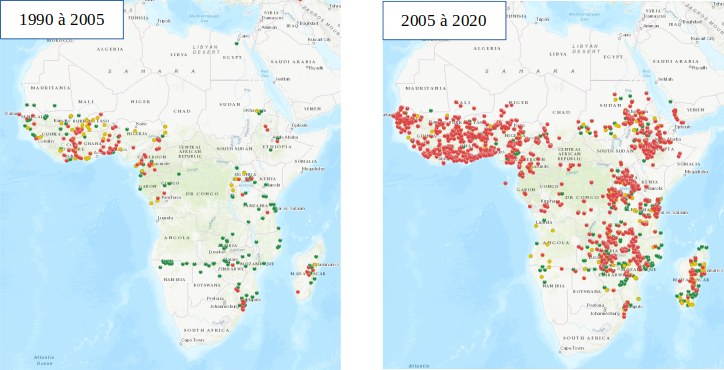
\includegraphics[width=1\linewidth]{figure/dev_res_phy} 

}

\caption[Distribution spatiale de l'émergence et expansion des résistances physiologiques des vecteurs aux insecticides]{Distribution spatiale des études confirmant une résistance aux insecticides chez les anophèles entre 1990 et 2005 (à gauche) et entre 2005 et 2020 (à droite) (source : IR Mapper www.irmapper.com)}\label{fig:dev-res-phy}
\end{figure}
\begin{figure}

{\centering 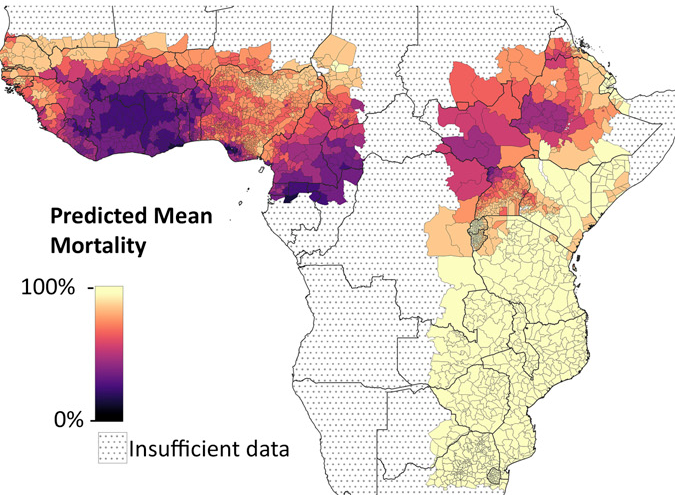
\includegraphics[width=0.5\linewidth]{figure/dev_res_phy_map} 

}

\caption[Distribution spatiale de la résistance à la deltaméthrine dans les populations d'An. gambiae s.l.]{Distribution spatiale de la résistance à la deltaméthrine dans les populations d'An. gambiae s.l. (\protect\hyperlink{ref-moyes_evaluating_2020}{Moyes et al., 2020})}\label{fig:dev-res-phy-map}
\end{figure}
\hypertarget{behavioural-resistance}{%
\subsubsection{Résistances comportementales}\label{behavioural-resistance}}

La résistance comportementale consiste en des modifications dans le comportement du moustique lui permettant de prévenir ou réduire les conséquences négatives des insecticides (\protect\hyperlink{ref-carrasco_behavioural_2019}{Carrasco et al., 2019}). La résistance peut être qualitative (modifications qui empêchent ou limitent le contact avec l'insecticide) ou quantitative (modifications qui arrêtent, limitent ou réduisent l'action de l'insecticide une fois le contact établi) (\protect\hyperlink{ref-carrasco_behavioural_2019}{Carrasco et al., 2019}). A ce jour, les mécanismes de résistance comportementale décrits dans la littérature sont principalement qualitatifs et consistent en des évitements spatiaux, temporels ou trophiques de l'insecticide. En particulier, dans les populations d'anophèles, les mécanismes de résistance qualitative comportementale suivants ont été décrits après la mise à l'échelle des outils de LAV à base d'insecticides (\protect\hyperlink{ref-manguin_residual_2013}{Durnez \& Coosemans, 2013}) : i) augmentation des comportements exophages ou exophiles (évitement spatial), ii) augmentation des comportements de piqûre précoce ou tardive (évitement temporel), iii) augmentation des comportements zoophages (évitement trophique).\\

Contrairement à la résistance physiologique, les mécanismes biologiques qui sous-tendent les résistances comportementales sont encore mal connus (\protect\hyperlink{ref-main_genetic_2016}{Main et al., 2016} ; \protect\hyperlink{ref-carrasco_behavioural_2019}{Carrasco et al., 2019} ; \protect\hyperlink{ref-manguin_residual_2013}{Durnez \& Coosemans, 2013}, ~; \protect\hyperlink{ref-killeen_characterizing_2014}{Gerry F. Killeen, 2014}). En particulier, il reste à comprendre si les changements de comportement reflètent des adaptations évolutives en réponse à la pression induite par les insecticides utilisés dans la LAV, comme pour les résistances physiologiques (\emph{résistance constitutive}) ou sont des manifestations d'une plasticité phénotypique préexistante qui se déclenche face à l'insecticide ou en réponse à une variation environnementale qui réduit la disponibilité des hôtes humains (\emph{résistance inductible})~; ces mécanismes n'étant pas mutuellement exclusifs (\protect\hyperlink{ref-manguin_residual_2013}{Durnez \& Coosemans, 2013}). Ces considérations peuvent avoir des implications importantes en matière d'efficacité sur le long terme des outils de LAV actuels. En effet, la résistance inductible pourrait impliquer que les vecteurs retrouvent rapidement leurs comportements de base lorsque les interventions de LAV sont modifiées, tandis que la résistance constitutive (héréditaire), qui pourrait impliquer que les vecteurs sensibles soient peu à peu remplacés par des vecteurs résistants, pourrait éroder progressivement et durablement l'efficacité des outils de LAV actuels. Certaines études récentes tendent à montrer qu'il pourrait y avoir une composante héréditaire à ces comportements résistants chez \emph{An. arabiensis} (\protect\hyperlink{ref-govella_heritability_2021}{Govella, Johnson, Killeen, \& Ferguson, 2021}).\\

Les résistances comportementales sont à ce jour, dans l'ensemble, moins étudiées que les résistances physiologiques (mécanismes biologiques sous-jacents moins compris, distributions spatio-temporelles moins rapportées, etc.) (\protect\hyperlink{ref-carrasco_behavioural_2019}{Carrasco et al., 2019}). A notre connaissance, une seule revue systématique des données existantes à l'échelle de l'Afrique a été effectuée (\protect\hyperlink{ref-sherrard-smith_mosquito_2019}{Sherrard-Smith et al., 2019}). Cette étude rapporte, entre autres, les variations spatiales et temporelles des taux d'endophagie (et donc exophagie) des vecteurs : elle montre notamment qu'à l'échelle de l'Afrique, la proportion des piqûres de moustiques effectuées à l'extérieur des habitations a augmenté de presque 10 \% entre 2003 et 2018 (figure \ref{fig:dev-res-comp}), et qu'une telle augmentation de l'exophagie pourrait résulter en un accroissement significatif de l'incidence du paludisme à l'échelle du continent (+ 10,6 millions de cas annuels).\\
\begin{figure}

{\centering 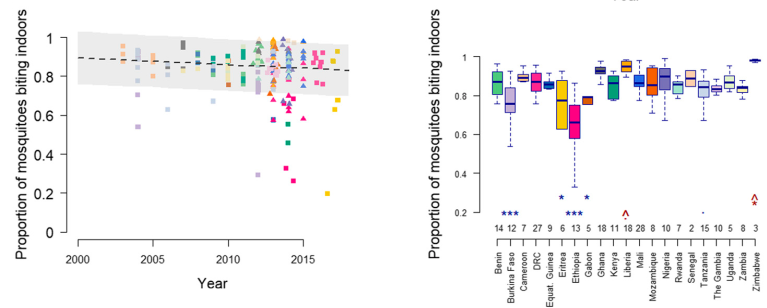
\includegraphics[width=1\linewidth]{figure/dev_res_comp} 

}

\caption[Distribution spatio-temporelle du taux d'endophagie des anophèles en Afrique]{Distribution temporelle (en haut) et spatiale (en bas) du taux d'endophagie des anophèles en Afrique (\protect\hyperlink{ref-sherrard-smith_mosquito_2019}{Sherrard-Smith et al., 2019})}\label{fig:dev-res-comp}
\end{figure}
\hypertarget{transmission-ruxe9siduelle-du-paludisme}{%
\subsection{Transmission résiduelle du paludisme}\label{transmission-ruxe9siduelle-du-paludisme}}

Les différentes limites des principaux outils de LAV aujourd'hui utilisés expliquent donc que la transmission continue de s'effectuer malgré la mise en oeuvre de ces interventions. La transmission qui persiste après avoir atteint une couverture universelle complète en MIILDA et/ou PID est appelée \emph{transmission résiduelle} du paludisme (\protect\hyperlink{ref-killeen_characterizing_2014}{Gerry F. Killeen, 2014}).\\

On peut envisager deux scenarii d'évolution de l'intensité de transmission résiduelle suite à l'introduction de MIILDA ou PID (\protect\hyperlink{ref-killeen_characterizing_2014}{Gerry F. Killeen, 2014}). Dans les deux scénarii, dans un premier temps l'intensité de la transmission diminue, jusqu'à atteindre un palier bas, sans disparaitre totalement à cause des limites inhérentes aux outils. Dans un second temps :
\begin{itemize}
\tightlist
\item
  soit \textbf{l'intensité de la transmission reste stable} (scenario 1), car :
  \begin{itemize}
  \tightlist
  \item
    les outils de LAV restent largement utilisés ;
  \item
    les résistances comportementales des vecteurs sont induites (la fraction de vecteurs échappant aux outils de LAV reste donc stable)
  \end{itemize}
\item
  soit \textbf{l'intensité de la transmission réaugmente} (rebond de la transmission) (scénario 2), à cause de :
  \begin{itemize}
  \tightlist
  \item
    une diminution progressive des taux d'utilisation des outils de LAV (par exemple, à cause d'une réduction des financements publics, ou de réticenses de la population à utiliser les interventions) ;
  \item
    et/ou une augmentation progressive de la prévalence des vecteurs physiologiquement résistants ;
  \item
    et/ou une augmentation progressive de la prévalence des vecteurs comportementalement résistants (dans ce scénario, les résistances comportementales sont donc constitutives) ;
  \item
    et/ou une modification progressive de la composition spécifique des vecteurs, vers des espèces davantage exophages ou piquant précocement ou tardivement.
  \end{itemize}
\end{itemize}
\begin{figure}

{\centering 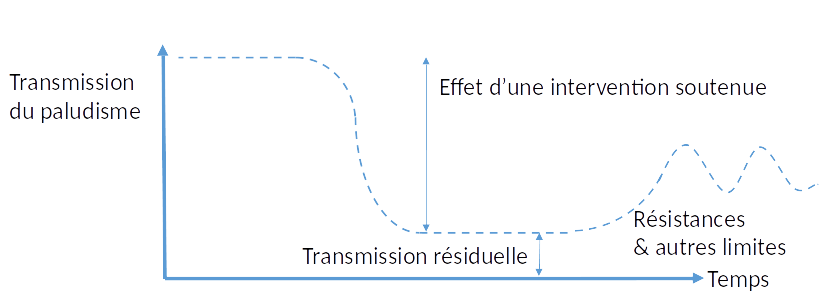
\includegraphics[width=0.9\linewidth]{figure/tr_schema} 

}

\caption[Concept de transmission résiduelle du paludisme]{Concept de transmission résiduelle du paludisme (adapté de (\protect\hyperlink{ref-killeen_characterizing_2014}{Gerry F. Killeen, 2014}))}\label{fig:tr-schema}
\end{figure}
Ces différentes problématiques concernant la transmission résiduelle du paludisme nous amènent ainsi à la présentation des enjeux et objectifs de la présente thèse.

\hypertarget{enjeux-objectifs-these}{%
\section{Enjeux, objectifs, organisation de la thèse}\label{enjeux-objectifs-these}}

\hypertarget{mesurer-et-caractuxe9riser-comprendre-pruxe9dire-le-risque-le-risque-de-transmission-ruxe9siduelle-du-paludisme}{%
\subsection{Mesurer et caractériser, comprendre, prédire le risque le risque de transmission résiduelle du paludisme}\label{mesurer-et-caractuxe9riser-comprendre-pruxe9dire-le-risque-le-risque-de-transmission-ruxe9siduelle-du-paludisme}}

Pour éviter les rebonds de transmission résiduelle, limiter leur impact, et plus largement redynamiser le progrès de la lutte contre le paludisme, plusieurs pistes sont proposées par la communauté des acteurs de la lutte contre le paludisme. En particulier, il est préconisé de concevoir de nouvelles interventions et méthodes de lutte, d'adapter les interventions au contexte local, et de cibler et prioriser le déploiement des interventions (\protect\hyperlink{ref-who_2020_world_nodate}{WHO, 2020}, \protect\hyperlink{ref-who_2021}{2021}). Afin de tendre vers ces objectifs opérationnels, il est d'une part nécessaire d'appronfondir certaines connaissances fondamentales sur les déterminants de la transmission résiduelle (par exemple, les mécanismes biologiques sous-jacents aux résistances comportementales). D'autre part, pour optimer et prioriser les interventions sur un territoire d'intérêt, il est important d'acquérir une connaissance fine du risque de transmission résiduelle, en particulier, de ses composantes, de son intensité, et de sa distribution spatio-temporelle sur ce territoire. Nous proposons ci-après trois approches, constituant autant d'enjeux de la thèse, permettant de générer des connaissances essentielles à ces effets. Ces approches visent respectivement à i) mesurer et caractériser le risque de transmission résiduelle, ii) comprendre ce risque, et iii) prédire ce risque.

\hypertarget{measure-risk}{%
\subsubsection{Approche n°1 : Mesurer et caractériser le risque}\label{measure-risk}}

Le risque de transmission résiduelle peut être défini comme la probabilité qu'un anophèle entre en contact avec un humain (autrement dit, probabilité de contact homme-vecteur), en zone couverte par les MIILDA ou PID. Bien que le simple contact avec l'humain ne soit pas suffisant pour transmettre le parasite (il faut par exemple, en sus, que l'anophèle soit infectieux, que la piqûre soit suffisamment longue, etc.), nous admettrons cette définition du risque de TR pour la suite de ce manuscrit. Le contact homme-vecteur se produit lorsque les anophèles sont à la recherche d'un repas de sang et que simultanément les hommes ne sont pas protégés par les moustiquaires. La probabilité de ce contact dépend donc en partie du comportement de l'anophèle - ses horaires et sites d'activités de recherche de repas de sang - et de celui de l'humain - son utilisation ou absence d'utilisation de moustiquaire, ses horaires d'utilisation de moustiquaires, ses habitudes nocturnes. En mesurant les comportements horaires anophéliens et humains au sein d'une même unité spatio-temporelle, il est possible de quantifier la probabilité de l'intéraction entre l'anophèle et l'humain : autrement dit, le risque de transmission résiduelle (\protect\hyperlink{ref-Garrett-Jones_1964}{Garrett-Jones \& Organization, 1964}; \protect\hyperlink{ref-killeen_quantifying_2006}{Gerry F. Killeen et al., 2006}; \protect\hyperlink{ref-killeen_characterizing_2014}{Gerry F. Killeen, 2014}).\\

\textbf{L'approche descriptive du risque de transmission résiduelle (\emph{mesurer et caractériser le risque}) consiste donc à quantifier la probabibilité de contact homme-vecteur et caractériser les sites et horaires où s'effectue ce contact, en zone couverte par les MIILDA.}\\

Une méthode permettant l'étude des interactions comportementales entre les populations humaines et vectorielles en zone couverte par les MIILDA a été décrite par Gerry F. Killeen et al. (\protect\hyperlink{ref-killeen_quantifying_2006}{2006}) et améliorée par Geissbühler et al. (\protect\hyperlink{ref-geissbuhler_interdependence_2007}{2007}). Cette méthode requiert la collecte de données fines sur les comportements humains (possession, utilisation, et horaires d'utilisation, de moustiquaires) et vectoriels (abondances horaires des piqûres de vecteurs). Ces données sont ensuite introduites dans un modèle mathématique calculant l'exposition humaine horaire à la piqûre d'anophèle.\\

Ces données et cette approche permet de dégager de précieuses informations concernant la transmission résiduelle sur un territoire d'intérêt : taux de possession et utilisation globale des moustiquaires par la population, niveau de protection conféré par les moustiquaires, site (intérieur ou extérieur des habitations) et horaire (soir, nuit, matin) où la transmission résiduelle s'effectue, hétérogénéité spatio-temporelle du risque de transmission résiduelle. Sur la base de ces informations et connaissances, il sera possible d'élaborer des plans de gestion et outils efficaces : par exemple, programmer une campagne de distribution de moustiquaires (si les taux de possession sont faibles) ou d'information, éducation, communication à leur utilisation (si les taux d'utilisation sont faibles), ou encore déployer des interventions de LAV complémentaires à la MIILDA qui ciblent la part résiduelle de la transmission (cad. qui visent les vecteurs impliqués dans le risque de transmission résiduelle).\\

\hypertarget{explain-risk}{%
\subsubsection{Approche n°2 : Comprendre le risque}\label{explain-risk}}

Si l'approche descriptive présentée dans la section précédente permet de mesurer la probabilité de contact hôte-vecteur, elle ne permet pas de comprendre les raisons sous-jacentes de l'intensité et de la variabilité spatio-temporelle de cette intéraction. \textbf{L'approche explicative du risque de transmission résiduelle proposée ici consiste ainsi à identifier les déterminants de l'intensité et de l'hétérogénéité spatio-temporelle de la probabibilité de contact homme-vecteur, en zone couverte par les MIILDA.}\\

En géographie, le risque est souvent défini comme \emph{«la probabilité d'occurrence de dommage compte tenu des interactions entre facteurs d'endommagement (aléas) et facteurs de vulnérabilité. On peut ainsi résumer cette définition par une formule : risque = aléa × vulnérabilité\footnote{\url{http://geoconfluences.ens-lyon.fr/glossaire/risque-s}, consulté le 2022-01-12}»}. Le risque de transmission résiduelle du paludisme (selon la définition proposée dans la section précédente) fait intervenir deux protagonistes : l'anophèle et l'homme. Les facteurs d'aléa peuvent être définis comme ceux directement liés au vecteur, et les facteurs de vulnérabilité comme ceux directement dépendants de l'homme. Ainsi, les facteurs d'aléa sont par exemple :
\begin{itemize}
\tightlist
\item
  \emph{Abondance journalière des vecteurs} : la densité environnante de vecteurs augmente à priori la probabilité pour un homme d'entrer en contact avec un vecteur ;
\item
  \emph{Résistances physiologiques des vecteurs} : les vecteurs résistants aux insecticides ont une longévité accrue, augmentant ainsi à priori à la fois la probabilité pour ces vecteurs (qui vivront plus longtemps) de transmettre le parasite, et la densité globale des vecteurs ;
\item
  \emph{Résistances comportementales des vecteurs} : les vecteurs exophages ou piquant précocement ou tardivement échappent à la protection conférée par les MIILDA et augmentent donc à priori la probabilité de contact homme-vecteur.\\
\end{itemize}
Les facteurs de vulnérabilité sont par exemple :
\begin{itemize}
\tightlist
\item
  \emph{Possession et utilisation de moustiquaire} : La probabilité de posséder et utiliser une moustiquaire réduit à priori la probabilité de contact homme-vecteur ;
\item
  \emph{Horaires d'utilisation des moustiquaires} : Les horaires d'utilisation des moustiquaires modulent à priori la probabilité de contact homme-vecteur.
\item
  \emph{Qualité de l'habitat} : Des facteurs tels que l'utilisation de grillages au fenêtres empêchant les vecteurs d'entrer dans les maisons modulent à priori la probabilité de contact homme-vecteur.\\
\end{itemize}
Comprendre le risque de transmission résiduelle consiste à améliorer les connaissances sur les systèmes \{environnement - vecteur\} et \{environnement - hôte\} du système vectoriel : identifier les déterminants (environnementaux, génétiques, socio-économiques, etc.) de chacune de ces composantes du risque et la manière dont ils impactent la composante. En d'autre termes, il s'agit d'approfondir les connaissances fondamentales sur les déterminants du risque :
\begin{itemize}
\tightlist
\item
  Caractériser la niche écologique des vecteurs ;
\item
  Caractériser la niche ``d'activité'' des vecteurs en recherche d'hôte ;
\item
  Comprendre les conditions d'émergence et de développement des résistances aux insecticides au sein d'une population de vecteurs ;
\item
  Comprendre les conditions de possession et d'utilisation des moustiquaires par la population ;
\item
  etc.\\
\end{itemize}
Un des enjeux (et difficultés) de cette approche est son caractère holistique : pour chaque composante de risque, il ne s'agit pas uniquement d'étudier si et comment un facteur donné impacte cette composante, mais plutôt de comprendre de quelle manière l'ensemble des potentiels facteurs impacte de manière complexe, en conditions ``réelles'' (cad. de terrain), cette composante de risque. Cette connaissance holistique des déterminants des différentes composantes du risque peut permettre d'identifier les leviers d'actions les plus pertinents pour diminuer le risque de transmission résiduelle.\\

Cette analyse peut se réaliser à l'aide de données (sur les composantes de risque à expliquer et leurs déterminants potentiels) et de méthodes de modélisation statistique qui seront détaillées dans le chapitre 2 de ce manuscrit. De manière générale, les enjeux sont ici d'identifier, pour chaque composante du risque : i) ses déterminants (quels facteurs influencent les intensités observées et la variabilité spatio-temporelle ?), ii) l'importance relative de chaque déterminant dans le comportement de la composante de risque (quels sont les déterminants qui influencent le plus la composante~?), iii) l'effet respectif (relation fonctionnelle) de chaque déterminant sur la composante du risque (si la valeur d'un des déterminants change, comment va changer la valeur de la composante du risque ?), et iv) l'existence, la nature et l'effet de potentielles intéractions entre les déterminants (comment les intéractions entre les déterminants impactent-elles la composante de risque ?).

\hypertarget{predict-risk}{%
\subsubsection{Approche n°3 : Prédire le risque}\label{predict-risk}}

Les deux approches précédentes (décrire et comprendre le risque) permettent d'accroitre les connaissances sur les intéractions (systèmes) hôte-vecteur, hôte-environnement, et vecteur-environnement ; ces connaissances permettant à leur tour de définir des caractéristiques pour de nouveaux outils de LAV et d'envisager des interventions adaptées au contexte local. Mais une fois ces interventions définies, comment savoir où et quand les déployer sur l'ensemble du territoire ? Prédire spatio-temporellement le risque de transmission résiduelle permet de cibler et prioriser les lieux et moments pour le déploiement des actions de gestion. Cette troisième approche consiste à estimer les valeurs des composantes du risque de transmission (abondance des vecteurs, taux de vecteurs résistants, etc.), voire du risque en lui-même (nombre de piqures / homme ou probabilité de contact homme-vecteur), en tout point de l'espace et du temps pour lesquels les observations « terrain » de ces composantes ne sont pas disponibles.\\

\textbf{L'approche prédictive du risque de transmission résiduelle (\emph{prédire le risque}) consiste donc à prédire ou anticiper la probabibilité de contact homme-vecteur en tout point de l'espace et du temps.}\\

Concrètement, cette approche consiste à générer des cartes (éventuellement saisonnières) pour chaque composante du risque (par exemple, cartes de la distribution de l'abondance des vecteurs), ou un système d'alerte précoce qui permettra d'anticiper à courte ou moyenne échéance, dans l'espace et dans le temps, les composantes du risque. Ces outils permettront de prioriser les zones d'intervention pour d'éventuels outils de LAV complémentaires aux MIILDA, et d'anticiper précocement le besoin (éventuellement ponctuel) en ces interventions. Notons que les granularités (résolutions) spatiales et temporelles de la prédiction (ou les échéances d'anticipation) sont à définir en fonction de plusieurs caractéristiques et contraintes~: dynamiques spatio-temporelles observées pour la composante de risque, échelles opérationnelles envisageables pour le déploiement des mesures, disponibilité et granularité des données environnementales, etc.\\

Les liens entre les différentes composantes du risque et l'environnement permettent leur prédiction spatio-temporelle. L'estimation de la valeur d'une composante de risque en tout point de l'espace et du temps se réalise en deux étapes~: i) l'apprentissage des relations qui existent entre la composante de risque étudiée et l'environnement (sur le même principe que l'analyse explicative - à la différence près que, dans l'analyse prédictive, il n'est pas nécessaire d'expliciter ces liens) et ii) l'extrapolation de cet apprentissage en tous points de l'espace et du temps pour lesquels les données environnementales sont disponibles. Cette approche nécessite donc la collecte de données représentatives des composantes du risque à prédire (entomologiques et environnementales notamment) et peut se réaliser là aussi grâce à des méthodes de modélisation statistique.\\

\hfill\break

Nous avons résumé dans le tableau ci-dessous les trois approches proposées (mesurer, comprendre, prédire le risque) : enjeux, questions, données nécessaires, approches d'analyse des données, exemple de connaissances ou outils potentiellement générés, exemple d'enjeux opérationnels.\\
\begin{figure}

{\centering 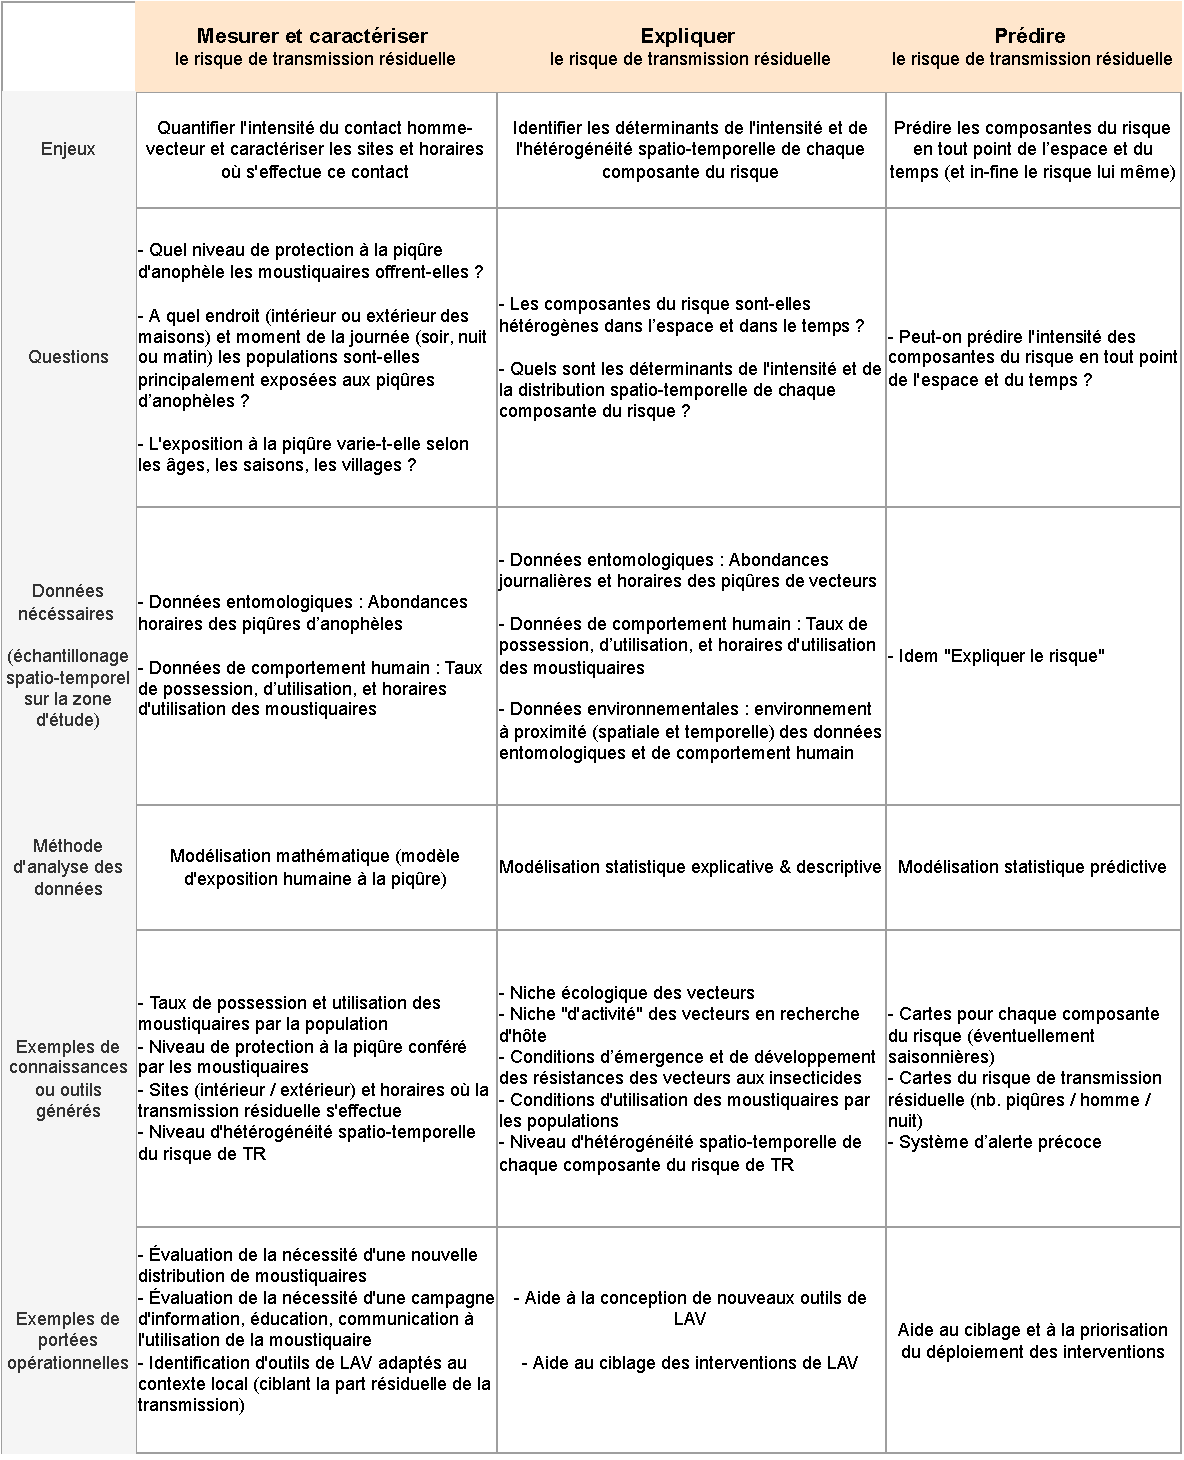
\includegraphics[width=1\linewidth]{tables/table_approches_tr} 

}

\caption[Enjeux et objectifs des trois approches théoriques pour décrire, comprendre et prédire le risque de transmission résiduelle du paludisme]{Enjeux et objectifs des trois approches théoriques pour décrire, comprendre et prédire le risque de transmission résiduelle du paludisme}\label{fig:table-approches-tr}
\end{figure}
\hypertarget{enjeu-de-la-thuxe8se-et-organisation-du-manuscrit}{%
\subsection{Enjeu de la thèse et organisation du manuscrit}\label{enjeu-de-la-thuxe8se-et-organisation-du-manuscrit}}

Cette thèse propose d'étudier, en implémentant en partie les approches décrites précédemment, le risque de transmission résiduelle du paludisme dans deux zones d'étude situées au Burkina Faso et en Côte d'Ivoire. Chaque zone recouvre environ la surface d'un district sanitaire rural ouest-africain (environ 2500 km\(^2\)). Ainsi, l'échelle spatiale d'étude est dite ``paysagère'' : autrement dit, nous travaillons à l'échelle du \emph{village} dans ces zones. L'enjeu d'ensemble est de montrer en quoi ces différentes approches apportent des éléments complémentaires permettant de proposer des stratégies de prévention adaptées aux contextes locaux.\\

Ce travail fera très largement appel à des méthodes avancées et non triviales issues de la science des données, en particulier la modélisation statistique. Aussi, à ces enjeux scientifiques s'en ajoute un davantage méthodologique, consistant à détailler les différentes manières dont la modélisation statistique peut servir la recherche scientifique ; et plus particulièrement à préciser son intérêt et potentiel dans l'étude des systèmes biologiques complexes tel que le système environnement-vecteur en conditions naturelles.\\

Les travaux de thèse s'articulent autour de quatre articles. Au total, deux de ces articles ont été rédigés en tant qu'auteur principal, et les deux autres ont été co-rédigés. Parmi les deux articles rédigés en auteur principal, l'un a été accepté et l'autre devrait être soumis prochainement. Les deux articles co-rédigés ont été acceptés. Tous les articles sont en anglais et sont donc préfacés dans ce manuscrit d'une introduction et d'un résumé en français.\\

Le manuscrit se compose de six chapitres faisant suite à ce premier chapitre introductif.\\

Le \textbf{chapitre \ref{data-mining}} (\textbf{\emph{Contexte méthodologique : Étude des systèmes complexes et modélisation statistique}}) a pour objectif de présenter et justifier la forme de raisonnement scientifique et l'approche méthodologique utilisée dans les principaux travaux de la thèse (chapitres 4 et 5). Nous y introduisons les différentes manières d'appréhender l'étude des systèmes biologiques complexes, et le rôle que peut tenir la modélisation statistique dans ce contexte. Nous élaborons sur les questions suivantes :
\begin{itemize}
\tightlist
\item
  Comment aborder l'étude des systèmes biologiques complexes tel que le système environnement-vecteur ? Quelles sont les deux approches existantes pour ce faire, et en quoi sont-elles complémentaires ?
\item
  A quoi sert la modélisation statistique ? En quoi cet ensemble d'outils et de méthodes permet-il d'appréhender les systèmes complexes, et au sens plus large, certains enjeux majeurs de la recherche scientifique (tester, consolider, créer des connaissances scientifiques ; prédire) ?
\item
  Quelles sont les différentes étapes d'un travail de modélisation statistique ?
\item
  En quoi les développements récents en science des données offrent-ils de nouvelles perspectives pour approfondir la compréhension des liens et intéractions dans les systèmes biologiques complexes, tels que le système environnement-vecteur ?\\
\end{itemize}
Le \textbf{chapitre \ref{data-collection-preparation}} (\textbf{\emph{Zones d'étude et préparation des données environnementales télédétectées}}) présente le projet dans lequel s'inscrit la thèse, les zones d'étude, et les travaux de production de certaines données environnementales utilisées dans les chapitres 4 et 5 (données paysagères et météorologiques produites à partir d'images satellitaires d'observation de la Terre).\\

Les chapitres 4 à 6 constituent le coeur de la thèse.\\

Au \textbf{chapitre \ref{data-mining-abundances}} (\textbf{\emph{Modélisation des dynamiques spatio-temporelles des abondances des vecteurs}}) (article n°1, auteur principal, publié), nous étudions la composante du risque ``Abondance journalière des vecteurs'' (autrement dit, la niche écologique des vecteurs). Nous expliquons (approche n°2) et évaluons la prédictibilité (approche n°3) des dynamiques spatio-temporelles des abondances journalières des principales espèces d'anophèles présentes dans nos deux zones d'études, en les modélisant avec des données environnementales issues de produits satellitaires d'observation de la Terre. Nous apportons des éléments de réponse aux questions suivantes :
\begin{itemize}
\tightlist
\item
  Les densités agressives des vecteurs sont-elles hétérogènes dans l'espace et dans le temps dans nos zones d'étude ?
\item
  Quels sont les déterminants des densités agressives pour chaque espèce majeure de vecteurs, et comment les impactent-ils~?
\item
  Est-on en mesure de prédire les densités agressives dans l'espace et dans le temps ?
\item
  Les déterminants considérés dans l'étude suffisent-ils à expliquer et prédire l'abondance des vecteurs et leur hétérogénéité spatio-temporelle dans nos zones d'étude ? Quels facteurs additionnels, non considérés dans l'étude, peuvent expliquer l'hétérogénéité des abondances ?\\
\end{itemize}
Au \textbf{chapitre \ref{data-mining-resistances}} (\textbf{\emph{Modélisation des dynamiques spatio-temporelles des résistances physiologiques et comportementales des vecteurs}}) (article n°2, auteur principal, à soumettre), nous étudions les composantes du risque ``Résistances physiologiques des vecteurs'' et ``Résistances comportementales des vecteurs'' (autrement dit, les conditions d'émergence et de développement de résistances des vecteurs aux insecticides). Nous expliquons (approche n°2) et évaluons la prédictibilité (approche n°3) des dynamiques spatio-temporelles des résistances physiologiques et des comportements des anophèles dans nos deux zones d'étude. En utilisant un nombre important de variables environnementales potentiellement explicatives des résistances, nous modélisons la probabilité individuelle de résistance physiologique des vecteurs ainsi que certains traits de leur comportement de piqûre (exophagie, agressivité précoce, agressivité tardive), afin d'apporter des éléments de réponse aux questions suivantes :
\begin{itemize}
\tightlist
\item
  Les résistances physiologiques et comportementales des vecteurs sont-elles hétérogènes dans l'espace et dans le temps dans nos zones d'étude~?
\item
  Quels sont les déterminants des résistances physiologiques et comportementales pour chaque espèce majeure de vecteurs, et comment les impactent-ils~?
\item
  Est-on en mesure de prédire les résistances physiologiques et comportementales dans l'espace et dans le temps ?
\item
  Les déterminants considérés dans l'étude suffisent-ils à expliquer et prédire les résistances des vecteurs et leur hétérogénéité spatio-temporelle dans nos zones d'étude ? Quels facteurs additionnels, non considérés dans l'étude, peuvent expliquer l'hétérogénéité des résistances ?\\
\end{itemize}
Le \textbf{chapitre \ref{complementary-studies}} (\textbf{\emph{Etudes complémentaires : contributions à des travaux de modélisation liés à la transmission du paludisme}}) (articles n°3 et 4, co-auteur, publiés) rassemble les deux études complémentaires auxquelles nous avons contribué dans le cadre de la thèse. Ces deux études concernent la zone d'étude située au Burkina Faso. Le premier article complémentaire (\emph{Modélisation de l'exposition humaine à la piqûre d'anophèles}) vise à mesurer et caractériser la transmission résiduelle (approche n°1) dans la zone d'étude. Le deuxième article complémentaire (\emph{Modélisation des dynamiques spatio-temporelles des cas de paludisme}) présente une étude visant à expliquer et prédire la distribution spatio-temporelle des cas de paludisme dans la zone d'étude, en utilisant des produits satellitaires d'observation de la Terre - comme pour les chapitres 4 et 5. Cette étude ne traite donc pas directement d'entomologie médicale, mais complémentairement aux études précédentes, permet d'illustrer la diversité des utilisations possibles des données satellitaires et modèles statistiques pour la gestion du paludisme sur le terrain.\\

Enfin, au \textbf{chapitre \ref{discussion}} (\textbf{\emph{Discussion générale}}), nous discutons l'ensemble des résultats. Nous proposons certaines stratégies pour la gestion du risque de transmission du paludisme sur nos deux zones d'étude. En particulier, nous faisons des propositions pour l'amélioration (i) des méthodes actuelles de lutte anti-vectorielle, (ii) de l'utilisation de la science et ingénierie des (géo-)données en général, et de la modélisation statistique en particulier, pour la recherche et le contrôle du paludisme, et (iii) des outils de surveillance et prévention du risque de transmission du paludisme à échelle locale en milieu rural ouest-africain.

\hypertarget{data-mining}{%
\chapter{Contexte méthodologique : Étude des systèmes complexes et modélisation statistique}\label{data-mining}}

L'enjeu des principales études de cette thèse (chapitres \ref{data-mining-abundances} et \ref{data-mining-resistances}) est d'approfondir les connaissances sur certains traits bio-écologiques, comportementaux ou physiologiques des vecteurs du paludisme. A cette fin, nous utiliserons une forme particulière d'étude des systèmes complexes, nommée ``holistico-inductive''. L'approche holistico-inductive est différente, conceptuellement et pratiquement, de l'approche hypothético-déductive généralement mieux maitrisée des chercheurs.\\

Qu'est ce que l'approche holistico-inductive, et en quoi diffère-t-elle de l'approche hypothético-déductive ? Quel rôle peut jouer la modélisation statistique dans ces différentes approches ? En quoi la modélisation statistique peut-elle servir les différents grands objectifs de la recherche scientifique : tester, améliorer, ou construire des théories scientifiques ? Ce chapitre apporte des éléments de réponse à ces questions. Son enjeu principal, dans le cadre strict de la thèse, est de préciser le raisonnement scientifique et les choix méthodologiques effectués dans les travaux à suivre. Au sens plus large, l'objectif est de montrer en quoi la modélisation statistique peut servir les différents grands objectifs de la recherche scientifique : tester, améliorer, ou - de part ses récents développements - construire des théories scientifiques.

\hypertarget{studying-complex-systems}{%
\section{Considérations épistémologiques sur l'étude des systèmes complexes}\label{studying-complex-systems}}

\hypertarget{les-deux-formes-dinfuxe9rence-logique-inductif-et-duxe9ductif}{%
\subsection{Les deux formes d'inférence logique (inductif et déductif)}\label{les-deux-formes-dinfuxe9rence-logique-inductif-et-duxe9ductif}}

L'objectif principal de la recherche scientifique est de faire avancer les connaissances en construisant et testant des hypothèses scientifiques. Les nouvelles hypothèses scientifiques sont construites à partir d'hypothèses existantes : ce processus s'appelle l'inférence logique. On reconnait deux formes principales d'inférence logique (\protect\hyperlink{ref-johnson-laird_human_2013}{Johnson-Laird, 2013}; \protect\hyperlink{ref-kell_here_2004}{Kell \& Oliver, 2004}) : la déduction et l'induction.\\

Le \textbf{raisonnement déductif} (ou \emph{hypothesis-driven} (\protect\hyperlink{ref-kell_here_2004}{Kell \& Oliver, 2004})) confirme l'hypothèse par le cas. Dans cette forme de raisonnement, l'hypothèse (ou la théorie) est le point de départ. Les observations (ou données) sont utilisées pour la tester dans des situations particulières et ainsi la vérifier ou l'infirmer.\\

Le \textbf{raisonnement inductif} (ou \emph{data-driven} (\protect\hyperlink{ref-kell_here_2004}{Kell \& Oliver, 2004})), à l'inverse, part du cas pour générer l'hypothèse. Dans cette forme de raisonnement, l'observation (ou la donnée) est le point de départ. Ces données sont utilisées pour formuler des hypothèses, des théories, plus générales. Autrement dit, dans ce cas, les données servent à générer l'hypothèse, qui est donc l'objectif et le point final du raisonnement.\\
\begin{lightcyanbox}
\begin{center}
Boite info n°1 : \textbf{Exemples de raisonnements déductif et inductif} (extrait de Kell \& Oliver (\protect\hyperlink{ref-kell_here_2004}{2004}))

\end{center}
Raisonnement déductif : Toutes les baleines sont bleues; Georges est une baleine, donc Georges est bleu.\\

Raisonnement inductif : Georges est une baleine et est bleu; Anne est une baleine et est bleue; Percy est une baleine et est bleue; etc.; nous pouvons donc induire l'idée (hypothèse) que toutes les baleines sont bleues.

\end{lightcyanbox}
Ces deux formes de raisonnement, à priori complémentaires, s'alimentent et forment ainsi le cycle de la génération de connaissances (figure \ref{fig:cycle-knowledge}). En particulier, elles tiennent chacun leur rôle dans l'étude des systèmes complexes.\\
\begin{figure}

{\centering 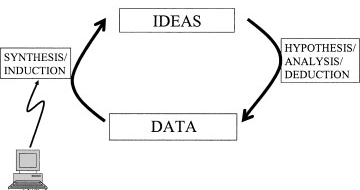
\includegraphics[width=0.6\linewidth]{figure/cycle_knowledge} 

}

\caption[Le cycle de la connaissance]{Le cycle de la connaissance (\protect\hyperlink{ref-kell_here_2004}{Kell \& Oliver, 2004})}\label{fig:cycle-knowledge}
\end{figure}
\hypertarget{study-complex-systems}{%
\subsection{Etudier les systèmes complexes : approches holistique et réductionniste}\label{study-complex-systems}}

Un système complexe est un sytème composé de nombreux éléments qui peuvent intéragir les uns avec les autres. S'il n'existe à priori pas de définition formelle largement acceptée du système complexe, ceux-ci sont définis, selon les cas et selon les auteurs, par l'existence d'effets et d'interactions non linéaires entre éléments du système, ou encore par l'existence de niveaux d'organisation différents (\protect\hyperlink{ref-bar-yam_general_nodate}{Bar-Yam, 2002}). Ainsi, par exemple, nous pouvons qualifier le système \{densités agressives des anophèles - environnement\} de complexe (figure \ref{fig:complex-system-anopheles}) : au sein de ce système, les effets de l'environnement sur le facteur étudié (la densités agressives des anophèles) peuvent être non-linéaires, de nombreuses interactions existent à priori (\protect\hyperlink{ref-stresman_beyond_2010}{Stresman, 2010}) ; l'ensemble provoquant un effet (les densités agressives) à priori difficilement prédictible. De manière générale, les sytèmes biologiques sont complexes (\protect\hyperlink{ref-bar-yam_general_nodate}{Bar-Yam, 2002}).\\

Deux stratégies au moins peuvent être envisagées pour étudier et tenter d'approfondir la compréhension d'un sytème complexe : l'approche réductionniste et l'approche holistique (\protect\hyperlink{ref-amboise_projet_1996}{Amboise \& Audet, 1996}; \protect\hyperlink{ref-bar-yam_general_nodate}{Bar-Yam, 2002}; \protect\hyperlink{ref-kell_here_2004}{Kell \& Oliver, 2004}). Nous résumons ces approches dans les prochains paragraphes, en nous basant sur ces trois références bibliographiques.\\

Dans l'approche réductionniste, le système complexe est considéré comme un ensemble de sous-sytèmes, moins complexes et ainsi plus simples à approcher, contenant un nombre réduit d'éléments, de relations et interactions. La compréhension de chacun de ces différents sous-systèmes permet ensuite de reconstruire le système complexe initial physiquement ou intellectuellement. Dans cette approche, le système complexe est tout d'abord décomposé en sous-systèmes pertinents en se basant sur les connaissances à priori du système complexe ; puis pour chaque sous-système, un nombre restreint de variables le caractérisant est sélectionné - là aussi en se basant sur les connaissances \emph{à priori}. L'enjeu de l'étude est alors de vérifier si et comment ces variables parcimonieusement sélectionnées impactent le comportement du sous-sytème. L'approche réductionniste repose donc sur un certain niveau de connaissance à priori du système complexe : à la fois pour créer les sous-sytèmes et pour sélectionner des variables pour chacun d'entre eux. En ce sens, l'approche réductionniste de l'étude des systèmes complexes est associée au raisonnement hypothético-déductif : les données servent à valider des hypothèses préalablement construites.\\

L'approche holistique, à l'opposé, considère que la complexité théorique des relations et interactions dans le système complexe implique qu'il faille étudier, chercher à décrire et comprendre, le système en entier, dans sa complexité. La première étape dans cette approche consiste à recueillir un maximum d'observations (données), ayant un impact plus ou moins lointainement soupçonné, sur le sytème étudié, quitte à en écarter certaines par la suite si elles ne s'avèrent pas utiles. Dans un second temps, les relations et interactions entre ces observations sont décrites - en général à l'aide d'outils informatiques et statistiques au regard du volume d'observations - puis interprétées à la lumière des connaissances préalables existantes. Cette démarche, reposant donc principalement sur les données, peut permettre d'améliorer, raffiner, ou faire émerger de nouvelles hypothèses scientifiques sur le fonctionnement du système complexe. En ce sens, l'approche holistique de l'étude des systèmes complexes est associée au raisonnement inductif : les données sont la source de l'hypothèse. On parle ainsi d'approche holistico-inductive.\\

\hfill\break
\begin{lightcyanbox}
\begin{center}
Boite info n°2 : \textbf{Exemple de questionnements de recherche et approches associées, en lien avec la thèse}

\end{center}
Répondre à la question \emph{``Sur mon territoire d'étude, quel est l'impact de l'interaction entre les précipitations et les températures sur les densités agressives des moustiques ?''} relève d'une approche réductionniste hypothético-déductive. Parmi tous les déterminants potentiels des densités agressives, deux en particulier sont sélectionnés (températures et précipitations), que l'on sait impacter l'abondance. L'objectif de l'étude sera de quantifier précisement l'impact des précipitations, des températures, et de leur interaction sur les densités agressives des moustiques.\\

Répondre à la question \emph{``Sur mon territoire d'étude, quels sont les déterminants des densités agressives des moustiques ?''} relève d'une approche holistico-inductive. L'objectif de l'étude sera de collecter un maximum d'observations sur l'ensemble des potentiels déterminants des densités agressives, puis de décrire les liens existant entre ces observations, afin d'élaborer des hypothèses sur les déterminants des densités agressives (facteurs déterminants, effets, interactions, etc.).

\end{lightcyanbox}
\hfill\break

L'approche hypothético-déductive réductionniste nécessite donc un cadre établi, rigide : l'hypothèse de recherche, précise, est formellement énoncée puis vérifiée ou testée à l'aide d'expérimentations contrôlées et de méthodes statistiques rigoureuses. L'approche hostistico-inductive, de son côté, est de prime abord moins rigide : les hypothèses de recherche ne sont pas formellement énoncées (ou n'existent même pas nécéssairement), le nombre de variables est plus important, les méthodes d'analyse moins rigides, le tout afin de laisser place à la découverte potentielle d'informations intéressantes. L'enjeu de l'approche holistico-inductive n'est pas de produire des résultats généralisables mais de mieux comprendre un phénomène d'intérêt, en espérant que la connaissance du phénomène acquise au cours de la recherche permettra de raffiner et d'améliorer la théorie existante. L'approche holistico-inductive requiert donc beaucoup de données et des hypothèses de départ très ouvertes. Le différentiel de rigidité au moment de l'établissement d'hypothèses préalables est regagné dans les étapes suivantes de l'analyse, qui nécéssitent rigueur, intégration du jugement subjectif et des connaissances humaines, afin d'interpréter les signaux (associations, etc.) révélés par l'analyse. En ce sens, ses défenseurs la considèrent comme une approche plus ouverte mais tout aussi rigoureuse que l'approche hypothético-déductive.\\

Ces deux approches de l'étude du système complexe, qui impliquent donc des démarches intrinsèquement différentes, sont pourtant complémentaires dans la compréhension des systèmes complexes. L'approche holistico-inductive, de part son caractère volontairement ouvert, est susceptible de soulever de nouvelles questions, ou hypothèses, potentiellement peu ou pas intuitionnées. La génération d'hypothèses est donc la fin du parcours. Ces nouvelles hypothèses pourront ensuite être testées expérimentalement, et validées, par raisonnement hypothético-déductif dans une approche réductionniste. Autrement dit, les approches hypothético-déductives (réductionnistes) et holistico-inductives sont itératives dans l'avancement des connaissances en général, et dans la compréhension des systèmes complexes en particulier (figure \ref{fig:holism-reductionism}).\\
\begin{figure}

{\centering 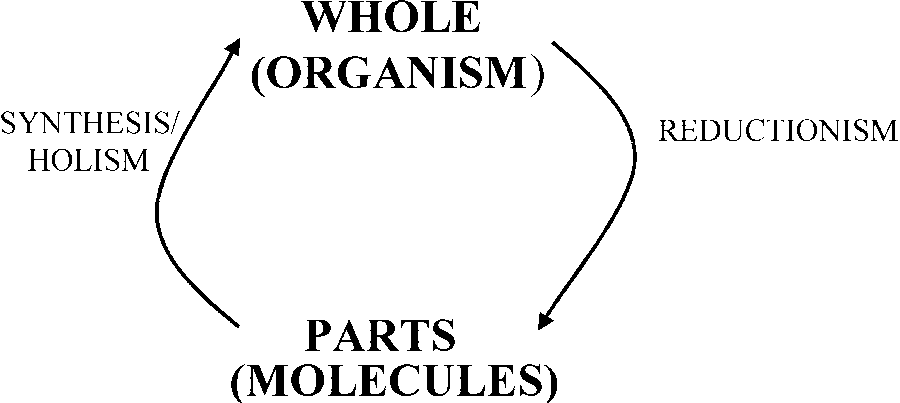
\includegraphics[width=0.6\linewidth]{figure/holism_reductionism} 

}

\caption[Holisme et réductionnisme en tant que stratégies complémentaires et itératives pour comprendre les systèmes complexes]{Holisme et réductionnisme en tant que stratégies complémentaires et itératives pour comprendre les systèmes complexes (\protect\hyperlink{ref-kell_here_2004}{Kell \& Oliver, 2004})}\label{fig:holism-reductionism}
\end{figure}
Bien que ces approches soient donc à priori complémentaires, plusieurs auteurs constatent que les approches inductive en général, et holistico-inductive en particulier, sont aujourd'hui moins utilisées dans la recherche scientifique que les approches hypothético-déductives et réductionnistes (\protect\hyperlink{ref-amboise_projet_1996}{Amboise \& Audet, 1996}; \protect\hyperlink{ref-bar-yam_general_nodate}{Bar-Yam, 2002}; \protect\hyperlink{ref-kell_here_2004}{Kell \& Oliver, 2004}; \protect\hyperlink{ref-shmueli_predictive_2010}{Shmueli \& Koppius, 2010}; \protect\hyperlink{ref-yanai_night_2019}{Yanai \& Lercher, 2019a}). L'approche hypothético-déductive est considérée dans certains milieux comme la seule méthode valable et fiable pour faire avancer les connaissances. Ainsi, par exemple, les rejets de projets ou idées scientifiques avec pour justification qu'ils ``n'ont pas d'hypothèse testée'', ou qu'ils consistent en des ``fishing expeditions'', sont fréquents : à l'extrême : ``s'il n'y a pas d'hypothèse, ce n'est pas de la science'' (\protect\hyperlink{ref-kell_here_2004}{Kell \& Oliver, 2004}; \protect\hyperlink{ref-yanai_night_2019}{Yanai \& Lercher, 2019a}). Cette préférence de la déduction sur l'induction est probablement liée à une forme de sécurité psychologique qu'offre l'approche déductive (\protect\hyperlink{ref-kell_here_2004}{Kell \& Oliver, 2004}) (si l'axiome et l'observation sont correctes, l'inférence logique doit être correcte) mais pas l'approche inductive ; ainsi qu'à son cadre en apparence plus rigoureux, formel (\protect\hyperlink{ref-amboise_projet_1996}{Amboise \& Audet, 1996}). Par ailleurs, nous hypothétisons ici que la défection pour l'approche holistico-inductive pourrait venir - en sus de son caractère inductif - d'un déficit de maitrise de certains outils nécéssaires à la conduite de cette approche (comme nous allons le voir dans la section \ref{statistical-modeling} à suivre) : l'analyse de données en général et les statistiques, mathématiques, informatique en particulier.\\

\hfill\break

Quoi qu'il en soit, ces paragraphes ont montré que l'analyse des données est au coeur de la génération et validation d'hypothèses en général et de l'étude des systèmes complexes en particulier, quelle que soit l'approche et la forme d'inférence logique utilisée. La modélisation statistique est un puissant outil d'analyse de données, capable de servir, historiquement, l'approche hypothético-déductive mais aussi, de part ses développements récents, l'approche holistico-inductive - en faisant donc un outil essentiel du chercheur.

\hypertarget{statistical-modeling}{%
\section{Les enjeux scientifiques de la modélisation statistique}\label{statistical-modeling}}

\hypertarget{formalisation-mathuxe9matique-du-moduxe8le-statistique}{%
\subsection{Formalisation mathématique du modèle statistique}\label{formalisation-mathuxe9matique-du-moduxe8le-statistique}}

L'approche déterministe de la science, défendue entre autre par Karl Popper (\protect\hyperlink{ref-arnaud_karl_1986}{Arnaud, 1986}), veut que la structure du monde est telle que tout \emph{évènement qui se produit} est déterminé par les \emph{événements passés} conformément aux \emph{lois de la nature}. Graphiquement et mathématiquement, cette approche peut être présentée par la figure \ref{fig:x-nature-y} et l'équation \emph{(1)} ci-dessous :
\begin{figure}

{\centering 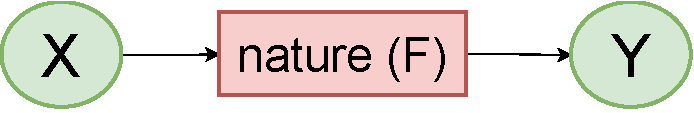
\includegraphics[width=0.5\linewidth]{figure/x_nature_y} 

}

\caption[Illustration de l'approche déterministe de la science ]{Illustration de l'approche déterministe de la science (adapté de (\protect\hyperlink{ref-breiman_statistical_2001}{Breiman, 2001b}))}\label{fig:x-nature-y}
\end{figure}
\begin{center}
(1)         $\mathrm{Y} = {F}(X)$ 
\end{center}
où :
\begin{itemize}
\tightlist
\item
  Y est l'évènement qui se produit,
\item
  \(X\) est l'ensemble des évènements passés causant Y,
\item
  \(F\) est la loi de la nature (aussi appelé modèle causal théorique) reliant \(X\) à Y.\\
\end{itemize}
La modélisation statistique est un outil permettant d'approximer et de formaliser mathématiquement cette réalité. Dans un modèle statistique, une ou plusieurs variables dite(s) `indépendante(s)', notées \(x\) et approximant X, sont associées à une autre variable dite `dépendante', notée y et approximant Y, via une fonction (le modèle statistique) notée \(f\). Mathématiquement, cela se traduit par l'équation suivante \emph{(2)} :\\
\begin{center}
(2)        $\mathrm{y} = {f}(x, \epsilon)$
\end{center}
\hfill\break

où :
\begin{itemize}
\tightlist
\item
  y est la variable dépendante, pendant de Y dans \emph{(1)},
\item
  \(x\) est une ou plusieurs variables indépendante(s), pendant de X dans \emph{(1)},
\item
  \(f\) est le modèle statistique associant y et \(x\), pendant de F dans \emph{(1)},
\item
  \(\epsilon\) est un terme d'erreur regroupant la part non expliquée de y, puisque \(f\) ne fait qu'approximer \(F\)
\end{itemize}
\hfill\break

Approximer et formaliser mathématiquement la réalité - cad. faire usage de la modélisation statistique - peut servir trois enjeux liés à \emph{(1)} : i) expliquer (tester) une loi de la nature \(F\), ii) décrire une loi de la nature \(F\), iii) prédire un évènement Y (\protect\hyperlink{ref-fayyad_data_nodate}{Fayyad, Piatetsky-Shapiro, \& Smyth, 1996}; \protect\hyperlink{ref-karpatne_theory-guided_2017}{Karpatne et al., 2017}; \protect\hyperlink{ref-shmueli_explain_2010}{Shmueli, 2010}; \protect\hyperlink{ref-shmueli_predictive_2010}{Shmueli \& Koppius, 2010}). En nous basant sur ces quatre références bibliographiques, nous résumons chacun de ces enjeux dans la prochaine section.\\

\hypertarget{les-trois-enjeux-de-la-moduxe9lisation-statistique-expliquer-pruxe9dire-duxe9crire}{%
\subsection{Les trois enjeux de la modélisation statistique (expliquer, prédire, décrire)}\label{les-trois-enjeux-de-la-moduxe9lisation-statistique-expliquer-pruxe9dire-duxe9crire}}

\emph{Note : au préalable, définissons dès maintenant les termes ``modélisation statistique'' et ``fouille de données'' tels qu'ils sont utilisés dans ce manuscrit. En effet, les définitions semblent varier selon les sources, au sein même de la famille des statisticiens. Nous définirons donc ``modélisation statistique'' comme l'ensemble du processus d'extraction de connaissances à partir de données et de modèle(s) statistique(s) (ledit processus est décrit dans la section \ref{steps-statistical-modeling}). Cette définition équivaut à celle de ``statistical modeling'' dans Shmueli (\protect\hyperlink{ref-shmueli_explain_2010}{2010}). Nous définirons ``fouille de données'' comme l'ensemble du processus d'extraction de connaissances à partir de données. Cette définition équivaut à celle de ``knowledge discovery in databases'' dans Fayyad et al. (\protect\hyperlink{ref-fayyad_data_nodate}{1996}). À la différence de la modélisation statistique, la fouille de données n'implique pas qu'il soit spécifiquement fait usage d'un modèle statistique pour générer des connaissances à partir des données.}

\hypertarget{moduxe9liser-pour-expliquer-moduxe9lisation-explicative}{%
\subsubsection{\texorpdfstring{\textbf{\emph{Modéliser pour expliquer (modélisation explicative)}}}{Modéliser pour expliquer (modélisation explicative)}}\label{moduxe9liser-pour-expliquer-moduxe9lisation-explicative}}

Un modèle statistique peut être utilisé pour \textbf{tester ou vérifier un modèle causal théorique (cad. des hypothèses) pré-existant}. On parle dans ce cas de `modélisation explicative' (\protect\hyperlink{ref-shmueli_explain_2010}{Shmueli, 2010}), `d'objectif de vérification' (\protect\hyperlink{ref-fayyad_data_nodate}{Fayyad et al., 1996}), ou de `theory-based model{[}ing{]}' (\protect\hyperlink{ref-karpatne_theory-guided_2017}{Karpatne et al., 2017}).\\

Dans cette approche, le modèle causal (cad. la loi de la nature) existe au niveau conceptuel, préalablement à l'utilisation du modèle statistique. Le modèle statistique est utilisé pour tester ou vérifier ce modèle théorique. Pour cela, des variables x et y, représentant respectivement X et Y, sont contruites à partir de données judicieusement collectées. Un modèle statistique est ensuite utilisé pour associer les variables x et y. L'interprétation du modèle statistique permet finalement de générer des informations statistiques sur le modèle causal théorique.\\

Cette forme de modélisation sert donc l'approche hypothético-déductive : les observations sont intégrées dans un modèle statistique dont l'objectif est de délivrer des informations statistiques sur les associations entre observations, permettant alors de vérifier et éventuellement préciser les hypothèses préalables. Dans l'étude des systèmes complexes, l'approche réductionniste fait donc ainsi usage de la modélisation explicative.\\

Ainsi, dans cette approche :
\begin{itemize}
\tightlist
\item
  \textbf{le modèle statistique \(f\) est l'objet d'intéret} de la modélisation : son analyse permet de \textbf{tester/vérifier} les hypothèses pré-existantes de \(F\) ;
\item
  les données \textbf{x et y sont des outils} permettant d'estimer \(f\).
\end{itemize}
\hypertarget{moduxe9liser-pour-duxe9crire-moduxe9lisation-descriptive}{%
\subsubsection{\texorpdfstring{\textbf{\emph{Modéliser pour décrire (modélisation descriptive)}}}{Modéliser pour décrire (modélisation descriptive)}}\label{moduxe9liser-pour-duxe9crire-moduxe9lisation-descriptive}}

Un modèle statistique peut être utilisé pour \textbf{décrire un modèle causal}. Dans ce cas, l'enjeu principal du modèle étant de décrire des associations entre des évènements, on parle de `modélisation descriptive' (\protect\hyperlink{ref-shmueli_explain_2010}{Shmueli, 2010}), d'objectif de `description' (\protect\hyperlink{ref-fayyad_data_nodate}{Fayyad et al., 1996}) ou `theory-guided data science model{[}ing{]}' (\protect\hyperlink{ref-karpatne_theory-guided_2017}{Karpatne et al., 2017}).\\

Dans cette approche, le modèle causal n'existe pas nécéssairement, ou n'est pas formellement établi, au niveau conceptuel. Le modèle statistique \(f\) est utilisé pour décrire un modèle théorique \(F\) contenant des associations éventuellement peu ou pas hypothétisées. L'interprétation du modèle statistique permet finalement, éventuellement de mieux comprendre \(F\).\\

Cette forme de modélisation sert donc l'approche holistico-inductive : les observations sont intégrées dans un modèle statistique dont l'objectif est de trouver des descriptions résumées et pertinentes expliquant les données. Le jugement subjectif et les connaissances préalables sur F permettent ensuite d'interpréter ces relations, afin d'améliorer les connaissances sur le modèle causal théorique.\\

Ainsi, dans cette approche :
\begin{itemize}
\tightlist
\item
  \textbf{le modèle statistique \(f\) est l'objet d'intéret} : son analyse permet éventuellement de \textbf{mieux comprendre} \(F\) ;
\item
  les données \textbf{x et y sont des outils} permettant d'estimer \(f\).
\end{itemize}
\hypertarget{moduxe9liser-pour-pruxe9dire-moduxe9lisation-pruxe9dictive}{%
\subsubsection{\texorpdfstring{\textbf{\emph{Modéliser pour prédire (modélisation prédictive)}}}{Modéliser pour prédire (modélisation prédictive)}}\label{moduxe9liser-pour-pruxe9dire-moduxe9lisation-pruxe9dictive}}

Enfin, un modèle statistique peut être utilisé pour \textbf{prédire de nouvelles ou futures valeurs d'un évènement}. On parle dans ce cas de modélisation statistique prédictive (\protect\hyperlink{ref-shmueli_explain_2010}{Shmueli, 2010}) ou d'objectif de prédiction (\protect\hyperlink{ref-fayyad_data_nodate}{Fayyad et al., 1996}).\\

La modélisation prédictive s'effectue en deux étapes. Dans un premier temps, un modèle statistique, dit prédictif, est construit à partir de données x et y. En général, le pouvoir prédictif du modèle est évalué, à savoir sa capacité à générer des prédictions précises sur de nouvelles observations\footnote{ce point est détaillé dans la section \ref{steps-statistical-modeling} à suivre}. Dans un second temps, ce modèle est utilisé pour prédire y lorsque de nouvelles valeurs de x, pour lesquelles les valeurs de y sont inconnues, sont disponibles.\\

La modélisation prédictive a donc principalement une portée opérationnelle : les prédictions sont généralement utilisées à des fins pratiques. Cependant, elle peut également jouer un rôle dans la construction ou amélioration de théories scientifiques. Utiliser un modèle statistique à des fins de prédiction, et évaluer son pouvoir prédictif, peut par exemple permettre d'évaluer la pertinence d'une théorie (cad. un modèle causal \(F\)) (si le modèle prédit mal, la théorie est-elle réellement valable ?), d'évaluer la prédictibilité d'un phénomène empirique, de comparer plusieurs théories concurrentes (celle qui prédit le mieux a des chances d'être celle qu'il faut retenir), d'améliorer les théories existantes, etc. (\protect\hyperlink{ref-shmueli_predictive_2010}{Shmueli \& Koppius, 2010}). Utilisée dans ce contexte, la modélisation prédictive rejoint donc en partie les enjeux de la modélisation descriptive.\\

Ainsi, dans cette approche :
\begin{itemize}
\tightlist
\item
  les données \textbf{x et y sont les objets d'intérêt}, en particulier y ;
\item
  \textbf{le modèle statistique \(f\) est un outil} permettant de générer des prédictions de y à partir de x.\\
  \strut \\
  \strut \\
\end{itemize}
Les rôles et fonctions du modèle statistique \(f\) et des données x et y diffèrent donc selon l'enjeu de la modélisation. Ces distinctions entre objets d'intérêt et outils sont importantes car elles guident les choix durant tout le processus de modélisation statistique, dès la phase de définition de l'objectif de l'étude. Dans la prochaine section, nous détaillons les grandes étapes du processus de modélisation statistique, en précisant pour chacune d'elles les différences fondamentales entre les formes de modélisation.

\hypertarget{steps-statistical-modeling}{%
\subsection{Les étapes du processus de modélisation statistique}\label{steps-statistical-modeling}}

Quelle que soit l'approche, le travail de modélisation statistique est un processus complexe, itératif, constitué d'étapes bien définies. Chacune de ces étapes implique des choix, qui diffèrent suivant l'approche utilisée, et ces choix peuvent avoir un impact sur les étapes suivantes et sur l'information et la connaissance extraites en bout de processus (\protect\hyperlink{ref-fayyad_data_nodate}{Fayyad et al., 1996}; \protect\hyperlink{ref-shmueli_explain_2010}{Shmueli, 2010}). La figure \ref{fig:modeling-steps} expose ces étapes. Dans cette section, nous énumérons et décrivons brièvement les principales d'entre elles, en exposant en quoi les choix diffèrent en fonction de l'approche empruntée. Sauf mention spécifique, l'ensemble de cette section est basée sur les travaux de Shmueli (\protect\hyperlink{ref-shmueli_explain_2010}{2010}), Shmueli \& Koppius (\protect\hyperlink{ref-shmueli_predictive_2010}{2010}) et Fayyad et al. (\protect\hyperlink{ref-fayyad_data_nodate}{1996}).\\
\begin{figure}

{\centering 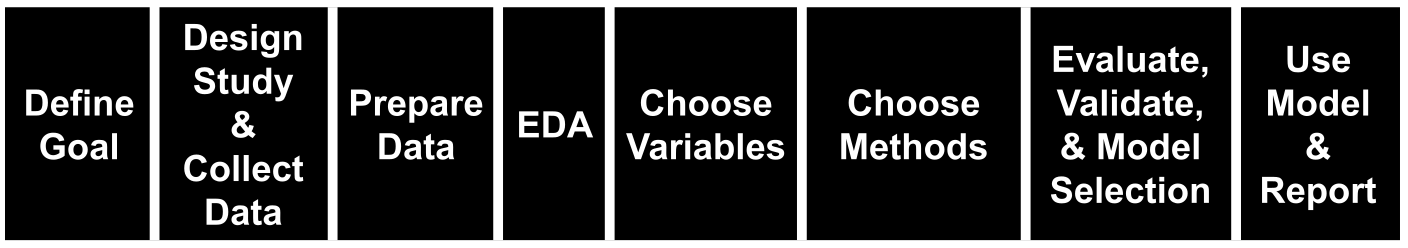
\includegraphics[width=1\linewidth]{figure/modeling_steps} 

}

\caption[Etapes du processus de modélisation statistique]{Etapes du processus de modélisation statistique (\protect\hyperlink{ref-shmueli_explain_2010}{Shmueli, 2010})}\label{fig:modeling-steps}
\end{figure}
\textbf{\emph{Définition de l'objectif}} : \textbf{Cette étape consiste à définir l'objectif à priori du travail de modélisation (expliquer, décrire, ou prédire).} En effet, les différences conceptuelles entre les trois approches de modélisation impliquent, comme nous allons le voir ensuite, des choix différents dans les étapes du processus de modélisation à suivre ; même si les données utilisées peuvent être identiques.\\

\textbf{\emph{Conceptualisation de l'étude et collecte des données}} : \textbf{Cette étape consiste à définir les caractéristiques de la collecte de données.} En fonction de l'approche, ces caractéristiques peuvent différer. Ainsi par exemple, en modélisation explicative, la puissance statistique est un critère majeur. Un certain nombre d'observation est donc nécéssaire, mais au delà d'un certain volume, la puissance statistique n'augmente plus. En modélisation prédictive, en général, davantage d'observations sont nécéssaires. D'autres enjeux sont à considérer : plans d'échantillonage des données, conditions d'expérimentation (laboratoire ou terrain), instruments de collecte des données, etc.\\

\textbf{\emph{Choix et construction des variables}} : \textbf{Cette étape consiste à construire des variables statistiques à partir des données.} Les critères pour construire les variables diffèrent largement selon l'approche. En modélisation explicative, l'objectif est la causalité : les variables x et y doivent donc représenter au plus proche les évènements X et Y que l'on cherche à vérifier. En modélisation prédictive, l'objectif est l'association : on ne cherche pas à comprendre le rôle de chaque variable en terme de relation de cause à effet. Les critères d'importance pour construire les variables sont donc principalement la qualité de l'association entre celles-ci et la disponibilité des variables prédictives (indépendantes), x, au moment des futures utilisations attendues du modèle (cad. quand il servira à prédire y à partir de nouveaux x).\\
\begin{lightcyanbox}
\begin{center}
Boite info n°3 : \textbf{Un exemple classique en géo-épidémiologie, le NDVI : variable explicative ou prédictive ?}

\end{center}
Une variable largement utilisée dans les travaux de modélisation statistique en géo-épidémiologie est le Normalized Difference Vegetation Index (NDVI) (\protect\hyperlink{ref-parselia_satellite_2019}{Parselia et al., 2019}), calculé à partir de valeurs de réflectance des sols mesurées par les capteurs embarqués dans les satellites ou les drones. Cette variable, adimensionnelle, permet de déterminer la santé de la végétation en mesurant la teneur en chlorophylle des plantes. Elle est donc à la fois représentative de la quantité de végétation et de la présence d'eau, deux paramètres environnementaux ayant à priori un impact sur les traits de vie des moustiques vecteurs (voir figure \ref{fig:complex-system-anopheles}). Cette variable a donc un fort potentiel d'association avec la densité des moustiques, et à ce titre, peut être utilisée en modélisation prédictive de leur abondance. En revanche, en modélisation explicative, cette variable est peu pertinente : i) on ne peut discriminer l'effet de la présence d'eau et de la végétation et ii) quel que soit le sens de l'association, il est possible de fournir une explication (une association positive peut être expliquée par la présence d'eau, une association négative peut être expliquée par la densité de végétation impliquant une réduction de la capacité de dispersion des moustiques (\protect\hyperlink{ref-le_goff_low_1997}{Le Goff, Carneval, \& Robert, 1997})). On lui préfèrera ainsi, en modélisation explicative, des variables plus proches du modèle causal théorique : quantités de précipitations, suface occupée par la végétation, etc.

\end{lightcyanbox}
En sus de la pertinence des variables, une autre distinction de taille est la gestion de la multicollinéarité (collinéarité entre variables). En modélisation explicative, la multicollinéarité est problématique car elle peut conduire à des effets (par ex. coefficients de régression) ou intervalles de confiance biaisés, interférant avec l'inférence. En modélisation prédictive, l'interprétation du modèle n'étant pas nécéssaire, la multicollinéarité n'est en général pas problématique.\\

\textbf{\emph{Choix du modèle statistique}} : \textbf{Cette étape consiste à sélectionner un modèle statistique, à savoir, une fonction mathématique ou un algorithme qui associe y à x.} Il existe de très nombreux modèles statistiques, et le choix dépend là encore de l'approche. En modélisation explicative et descriptive, où l'objectif est d'analyser \(f\), le critère principal de Sélection est l'interprétabilité du modèle, c'est-à-dire la capacité à extraire les associations que le modèle a capturées. En modélisation explicative, le modèle doit être en mesure de délivrer des informations statistiques précises et chiffrées (intensité de l'effet, significativité de l'association, etc.). En modélisation descriptive, le modèle doit être en mesure de capturer au mieux les relations et interactions, potentiellement complexes (non-linéaires), entre variables. En modélisation prédictive, où \(f\) n'est que l'outil, l'enjeu est de sélectionner un modèle qui génèrera les meilleures prédictions possibles de y ; l'interprétabilité du modèle n'est donc pas un critère de choix. L'interprétabilité et interprétation des modèles statistiques sont intrinsèquement liés à leur nature et la manière dont chacun fonctionne pour associer les variables. Nous nous attardons sur les différentes philosophies d'associations entre variables et sur l'interprétation des modèles dans les sections \ref{model-categories} et \ref{model-interpretation}.\\

\textbf{\emph{Validation du modèle}} : \textbf{Cette étape consiste à vérifier certaines hypothèses permettant d'utiliser ou d'interpéter le modèle correctement.} En modélisation explicative, la validation du modèle consiste à vérifier que la forme de \(f\) représente adéquatement la relation à priori entre x et y (voir section \ref{model-categories}). En modélisation prédictive, la validation consiste à évaluer la propension du modèle à généraliser l'apprentissage, c'est à dire, à ne pas avoir sur-appris\footnote{le surraprentissage est la propension du modèle à s'ajuster trop proche des données qui ont été utilisées pour l'entraîner - provoquant ainsi son incapacité à prédire sur de nouvelles données x}.\\

\textbf{\emph{Evaluation du modèle}} : \textbf{Cette étape consiste à évaluer la puissance explicative ou prédictive du modèle.} En modélisation explicative, la puissance explicative du modèle est la force de la relation indiquée par \(f\). Des mesures telles que le R\(^{2}\), représentant la proportion de la variance d'une variable dépendante expliquée par les variables indépendantes, peuvent être rapportées. En modélisation prédictive, la puissance prédictive du modèle est la capacité du modèle à prédire sur de nouvelles données, non utilisées pour entrainer le modèle. Là aussi, des indicateurs mesurant l'écart entre les valeurs observées et prédites peuvent être utilisées (aire sous la courbe (AUC), erreur moyenne carrée (MSE), etc.). Le choix de l'indicateur de puissance prédictive dépend de la nature et de la distribution statistique des données. Une différence majeure entre les évaluations des modèles prédictifs et explicatifs est la nature des données sur lesquelles l'évaluation est effectuée : alors qu'en modélisation explicative l'évaluation est faite sur les données ayant servi à générer le modèle, en modélisation prédictive, l'évaluation doit être faite sur des données qui n'ont pas servi à générer le modèle, puisque l'objectif du modèle sera de prédire sur de nouvelles données. Par ailleurs, si les observations sont non-indépendantes (par exemple dans le cas des enquêtes transversales ou des données spatiales ou temporelles), le jeu de données de validation d'un modèle prédictif doit être judicieusement sélectionné afin d'être indépendant du jeu de données d'entrainement - ceci afin d'éviter des performances prédictives surévaluées dues au suraprentissage (\protect\hyperlink{ref-meyer_improving_2018}{Meyer, Reudenbach, Hengl, Katurji, \& Nauss, 2018}).\\

\textbf{\emph{Sélection du modèle}} : \textbf{Cette étape consiste à sélectionner un modèle à interpréter ou utiliser parmi les différents modèles potentiellement valides.} En modélisation explicative, un des critères les plus cruciaux est l'importance théorique des variables dans le modèle causal \(F\). Il est ainsi nécéssaire de retenir dans le modèle les variables qui ont un effet théorique important, même s'il s'avère que dans le modèle ces variables sortent non-significativement associées à la variable réponse (\protect\hyperlink{ref-shmueli_explain_2010}{Shmueli, 2010}) (par exemple, il est important de retenir la variable `type de mesure de lutte anti-vectorielle implémentée' dans un modèle qui cherche à expliquer l'abondance des moustiques, même si cette variable n'est finalement pas statistiquement significativement associée à l'abondance). En modélisation prédictive, le premier critère est la performance prédictive du modèle. Le choix se portera donc sur le modèle qui génère la meilleure prédiction, quitte à supprimer des variables théoriquement importantes au niveau conceptuel. De nombreuses méthodes de Sélection automatique de variables en modélisation prédictive existent à cet effet.\\

\textbf{\emph{Interprétation du modèle et utilisation des résultats}} : \textbf{Cette étape consiste à finalement extraire de l'information ou de la connaissance pertinente à partir du modèle statistique.} En modélisation explicative, les informations d'intérêt sont les métriques statistiques renseignant sur l'effet des variables explicatives sur la variable à expliquer (coefficients directeurs par exemple), la significativité de l'effet (p-value par exemple), et la performances explicative du modèle (R\(^{2}\) par exemple). En modélisation descriptive, il s'agit de rapporter les relations, potentiellement complexes, capturées par le modèle sous une forme compréhensible par l'humain (tableaux, graphiques, etc.). En modélisation prédictive, l'interprétation du modèle est secondaire. Les informations d'intérêt sont principalement celles issues des étapes de validation et évaluation du modèle. Les concepts et outils d'interprétation des modèles, notamment en modélisation descriptive, sont détaillées dans la section \ref{model-interpretation}.\\

\hypertarget{model-categories}{%
\subsection{Les deux grandes familles de modèles statistiques (modèles paramétriques et non-paramétriques)}\label{model-categories}}

Le choix du modèle statistique est un des éléments primordial dans le processus de modélisation statistique. En effet, chaque modèle est défini de telle manière qu'intrinsèquement, il associe différemment les variables indépendantes (x) et dépendantes (y). En bout de chaine, cela peut avoir un impact considérable sur la nature de la connaissance qui est finalement extraite.\\

On peut distinguer deux grandes catégories de modèles statistiques, définies par deux philosophies d'association de y à x (cad. de construction de \(f\)) conceptuellement différentes (\protect\hyperlink{ref-breiman_statistical_2001}{Breiman, 2001b}) : les modèles paramétriques (que Breiman (\protect\hyperlink{ref-breiman_statistical_2001}{2001b}) appelle \emph{data model(s)}) et les modèles non-paramétriques (que Breiman (\protect\hyperlink{ref-breiman_statistical_2001}{2001b}) appelle \emph{algorithmic model(s)}).\\

Les modèles paramétriques simplifient la fonction \(f\) à une forme connue (par exemple : gaussienne, négative binomiale, etc.). Cette forme doit donc être spécifiée (par le modélisateur) dans le modèle. Le rôle du modèle statistique est ensuite d'estimer les coefficients de la fonction à partir des données. Des exemples de modèles paramétriques largement utilisés sont la régression linéaire et la régression logistique.\\

Les modèles non-paramétriques, de leur côté, ne font pas d'hypothèse concernant la forme de la fonction \(f\). Ces modèles cherchent à s'ajuster au mieux aux données en construisant la fonction f à partir des données. Des exemples de modèles non-paramétriques largement utilisés sont les arbres de décision (et modèles dérivés, tels que les forêts aléatoires) et \emph{Support Vector Machines}. Ces modèles sont parfois appelés modèles ou algorithmes d'apprentissage automatique (\emph{machine learning}) (\protect\hyperlink{ref-bzdok_statistics_2018}{Bzdok, Altman, \& Krzywinski, 2018}) ou de fouille de données (\emph{data mining}) (\protect\hyperlink{ref-shmueli_explain_2010}{Shmueli, 2010}).\\

Chacune de ces méthodes possède son lot d'avantages et d'inconvénients. Les modèles paramétriques sont transparents (les coefficients de \(f\) sont directement interprétables) et requièrent moins de données que les modèles non-paramétriques, puisque la forme de \(f\) est à priori determinée. Cependant, ils exigent que la forme de la fonction soit connue à l'avance, et sont ensuite contraints de se conformer à cette forme. Les modèles non-paramétriques, parce qu'ils doivent chercher de manière autonome la forme de \(f\), requièrent plus de données, de puissance et de temps de calcul, sont davantage susceptibles de surapprendre et sont moins transparents que les modèles paramétriques. Cependant, ils ne requièrent pas d'hypothèse à priori sur la forme fonctionnelle et sont capables de s'adapter à une gamme bien plus large de formes, en faisant ainsi de bons candidats si les relations sont à priori inconnues ou soupçonnées complexes (relations entre variables non-linéaires ou interactions potentielles), ce qui est souvent le cas dans les processus naturels et en particulier biologiques (\protect\hyperlink{ref-breiman_statistical_2001}{Breiman, 2001b}).\\

Aussi, par définition, les modèles paramétriques sont à priori adaptés à la modélisation explicative (modèle causal théorique connu, besoin de résultats statistiques) et les modèles non-paramétriques à la modélisation prédictive (flexibilité, performance) (\protect\hyperlink{ref-bzdok_statistics_2018}{Bzdok et al., 2018}; \protect\hyperlink{ref-shmueli_explain_2010}{Shmueli, 2010}). La modélisation descriptive, quand à elle, requiert à la fois un modèle flexible (puisque, par définition de cette approche de modélisation, les relations ne sont pas nécéssairement connues) et interprétable (puisque l'objectif final est l'extraction de connaissances à partir des relations que le modèle a capturées), deux propriétés à priori difficilement conciliables au regard de ce qui est écrit ci-dessus. Consciente du potentiel des modèles non-paramétriques pour la génération de connaissances (au delà de leur potentiel prédictif indiscutable), la communauté des scientifiques des données a developpé un ensemble d'outils visant à interpréter les associations que ces modèles capturent. La prochaine section présente le concept et quelques outils d'interprétation des modèles statistiques non-paramétriques.\\

\hypertarget{model-interpretation}{%
\subsection{L'interprétation des modèles statistiques non-paramétriques}\label{model-interpretation}}

L'interprétation des modèles statistiques est un élément fondamental du processus de modélisation, en particulier en modélisation explicative et descriptive. L'interprétation des modèles peut être définie comme l'extraction de connaissances pertinentes à partir d'un modèle statistique concernant des relations soit contenues dans les données soit apprises par le modèle (\protect\hyperlink{ref-murdoch_definitions_2019}{Murdoch, Singh, Kumbier, Abbasi-Asl, \& Yu, 2019}). Au niveau de l'interprétabilité, on distingue deux grandes catégories de modèles (\protect\hyperlink{ref-murdoch_definitions_2019}{Murdoch et al., 2019}) : les modèles permettant de comprendre naturellement et directement les relations qu'ils ont capturées, et les modèles nécéssitant une phase supplémentaire d'interprétation à postériori de leur génération, avec des outils spécifiques, pour extraire de l'information sur les relations qu'ils ont capturées.\\

La première catégorie de modèles (modèles directement interprétables) est constituée dans l'ensemble des modèles paramétriques. Ces modèles sont transparents : les coefficients de la fonction (ainsi que d'autres métriques telles que les intervalles de confiance) sont les outils d'interprétation du modèle, à partir desquelles les connaissances sont extraites.\\

La deuxième catégorie de modèles (modèles nécéssitant une phase supplémentaire d'interprétation) est constituée dans l'ensemble des modèles non-paramétriques. Ces modèles ont l'avantage d'être en capacité de capturer des relations et interactions complexes mais l'inconvénient de ne pas délivrer directement les relations qu'ils ont capturées, à tel point qu'il sont souvent considérés comme des boites noires (\protect\hyperlink{ref-bzdok_statistics_2018}{Bzdok et al., 2018}). Aussi, un ensemble d'outils dont l'objectif est d'extraire des informations sur les relations que le modèle a capturées a été développé depuis une vingtaine d'années (\protect\hyperlink{ref-molnar_interpretable_2019}{Molnar, 2019}).\\

Parmi les outils d'interprétation à postériori des modèles, on distingue deux grandes familles : les méthodes indépendantes du modèle interprété (dites ``model-agnostic'') et les méthodes spécifiques à un modèle donné (dites ``model-specific'') (\protect\hyperlink{ref-molnar_interpretable_2019}{Molnar, 2019}). Les méthodes agnostiques peuvent elle-mêmes être subdivisées en deux classes : les méthodes globales et méthodes locales (\protect\hyperlink{ref-murdoch_definitions_2019}{Murdoch et al., 2019}). Les méthodes globales décrivent la manière dont les variables indépendantes affectent la variable dépendante en moyenne, tandis que les méthodes locales visent à décrire l'effet des variables indépendante sur une observation individuelle (ou un groupe d'observations). Enonçons et expliquons le fonctionnement de deux des outils d'interprétation ``model-agnostic'' les plus anciens et utilisés (et utilisés en particulier dans les travaux de cette thèse) : l'importance des variables par permutation et les graphiques de dépendance partielle.\\

L'importance des variables par permutation (\emph{permutation feature importance}) est une méthode introduite en 2001 par Breiman (\protect\hyperlink{ref-breiman_random_2001}{Breiman, 2001a}). Cette méthode renseigne sur ``l'importance'' de chaque variable indépendante dans le modèle en mesurant l'augmentation de l'erreur de prédiction du modèle après avoir permuté les valeurs de la variable. Une variable est ``importante'' si la permutation aléatoire de ses valeurs augmente l'erreur du modèle, car dans ce cas, le modèle s'est appuyé sur la variable pour la prédiction. A l'inverse, une variable est ``sans importance'' si la permutation aléatoire de ses valeurs ne modifie pas l'erreur de prédiction du modèle, car dans ce cas, le modèle n'a pas considéré la variable pour la prédiction. Un exemple de graphique d'importance des variables est fourni à la figure \ref{fig:example-vip}.\\
\begin{figure}

{\centering 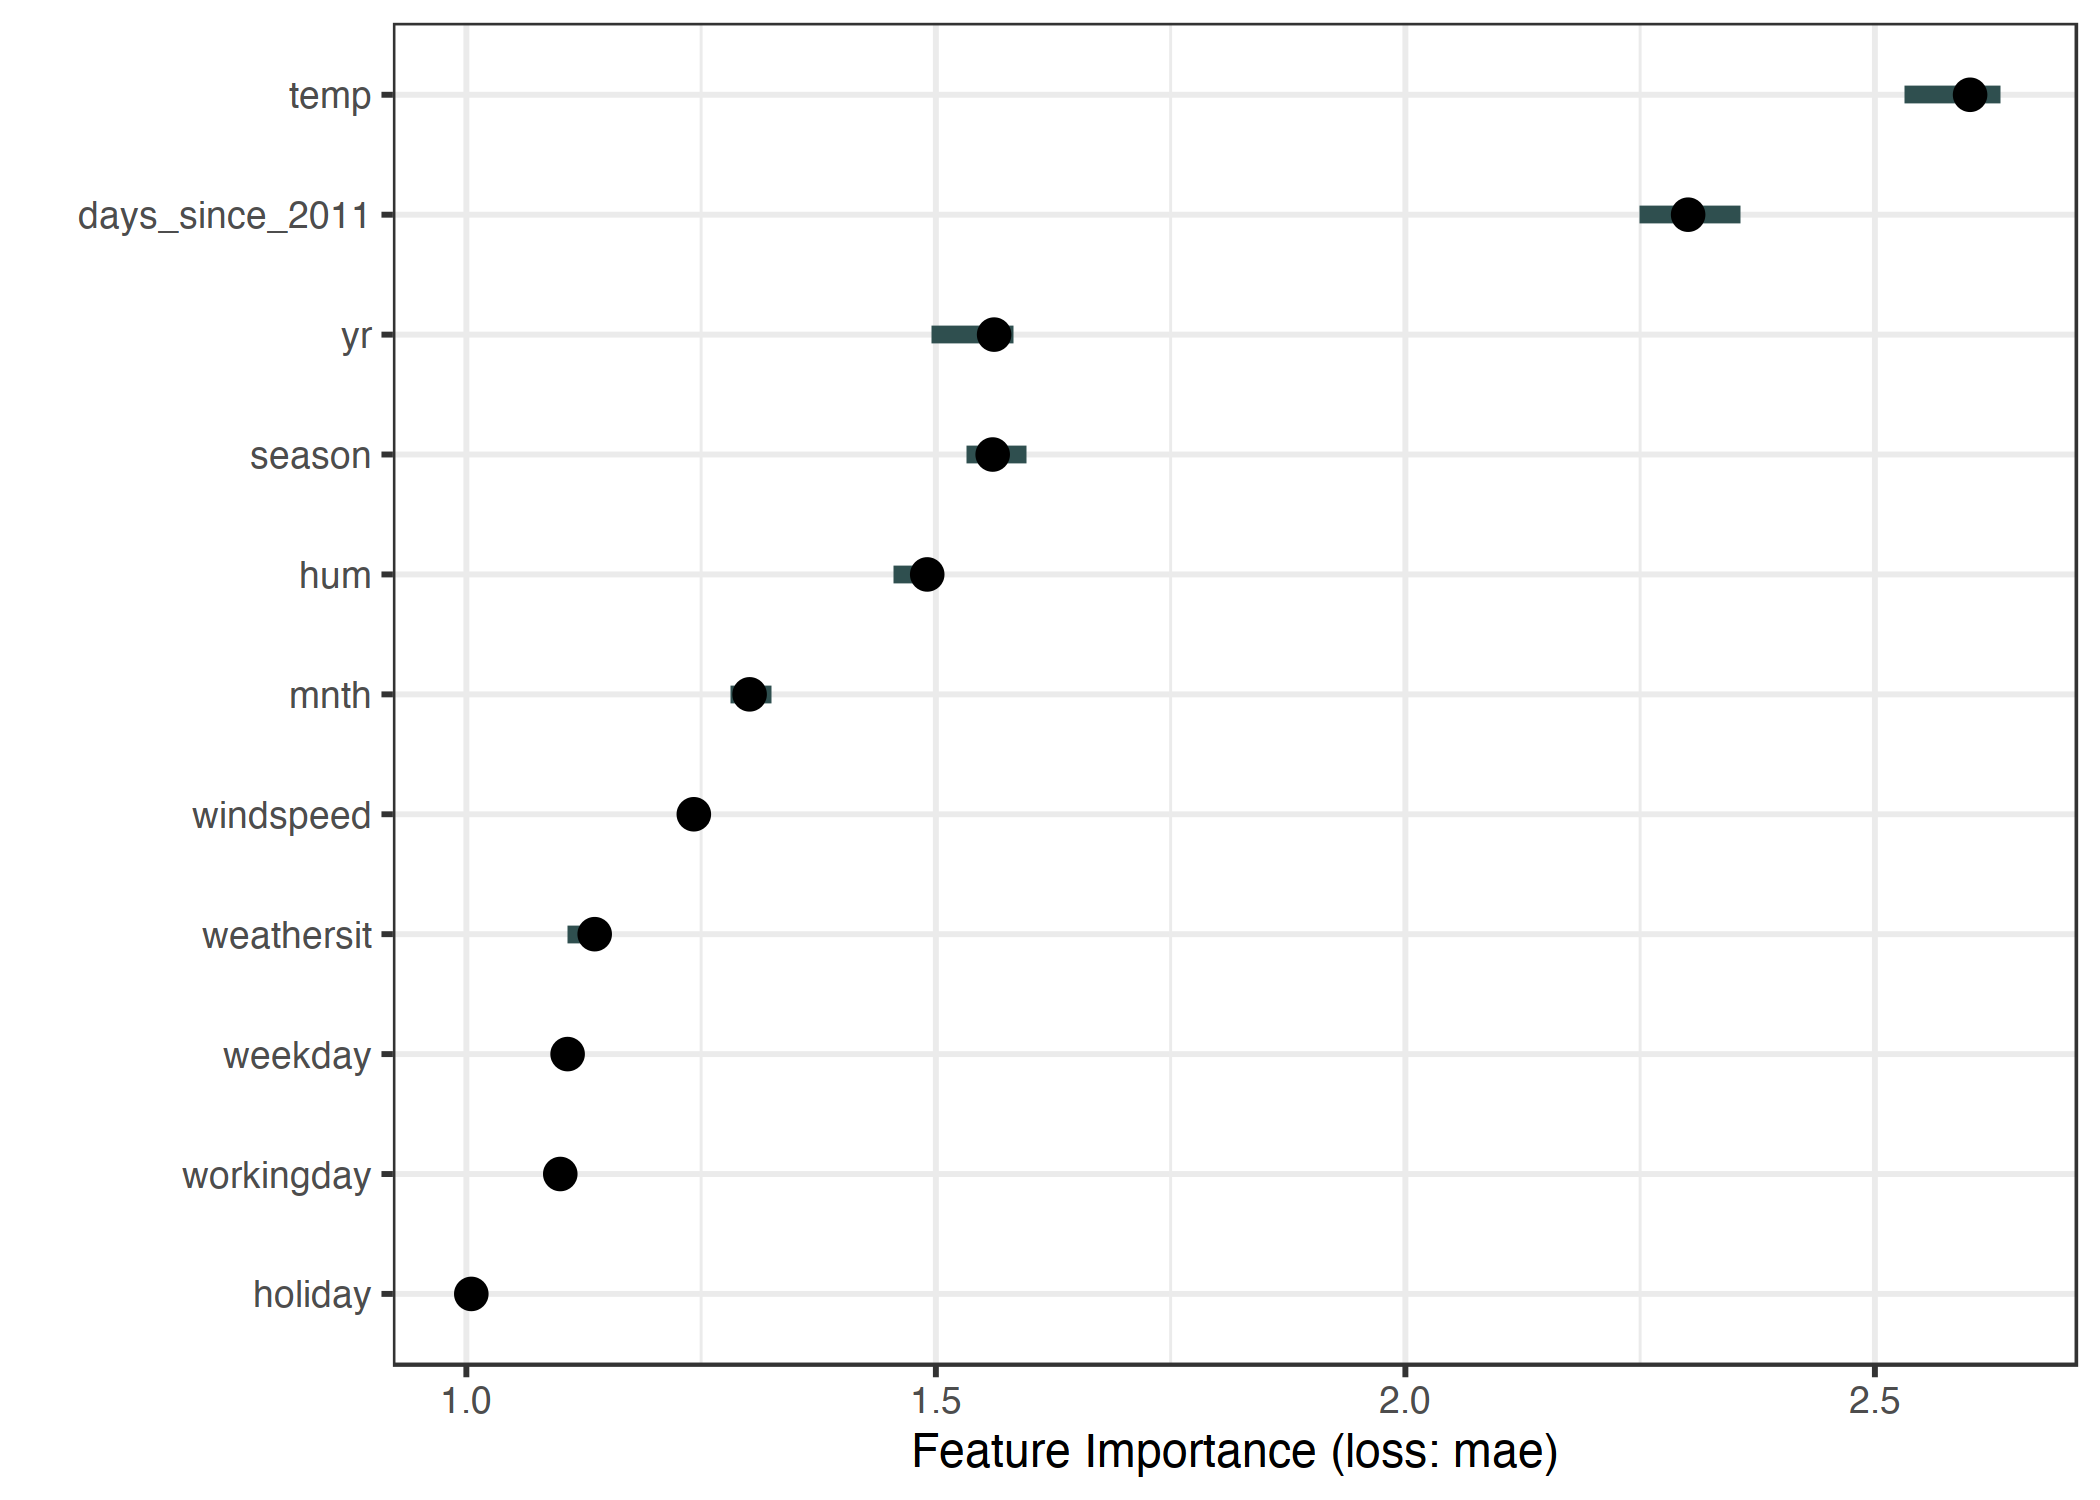
\includegraphics[width=0.7\linewidth]{figure/importance-bike-1} 

}

\caption[Exemple de graphique d'importance des variables]{Exemple de graphique d'importance des variables extrait de (\protect\hyperlink{ref-molnar_interpretable_2019}{Molnar, 2019}). Le modèle statistique sous-jacent prédit un nombre de vélos loués en fonction d'un ensemble de paramètres météorologiques et socio-économiques. Le graphique montre que la variable la plus importante est la température. Par extension, on peut donc émettre l'hypothèse que la température est le facteur principal impactant la location de vélos.}\label{fig:example-vip}
\end{figure}
Les graphiques de dépendance partielle (\emph{partial dependence plots} (PDP)), de leur côté, ont été introduits en 2001 par Friedman (\protect\hyperlink{ref-friedman_greedy_2001}{Friedman, 2001}). Cette méthode renseigne sur la relation fonctionnelle entre une variable indépendante et la variable dépendante. La relation fonctionnelle est calculée en fixant tour à tour chacune des valeurs de la variable indépendante d'intérêt pour toutes les observations, puis en calculant la valeur de la variable dépendante ainsi prédite par le modèle. Un graphique de dépendance partielle peut montrer si la relation entre la variable dépendante et indépendante est linéaire, monotone ou plus complexe. On peut utiliser la même méthode avec deux variables indépendantes : dans ce cas, le graphique renseigne sur l'effet de l'interaction entre ces deux variables indépendantes sur la variable dépendante. Un exemple de graphique de dépendance partielle est fourni à la figure \ref{fig:example-pdp}.\\
\begin{figure}

{\centering 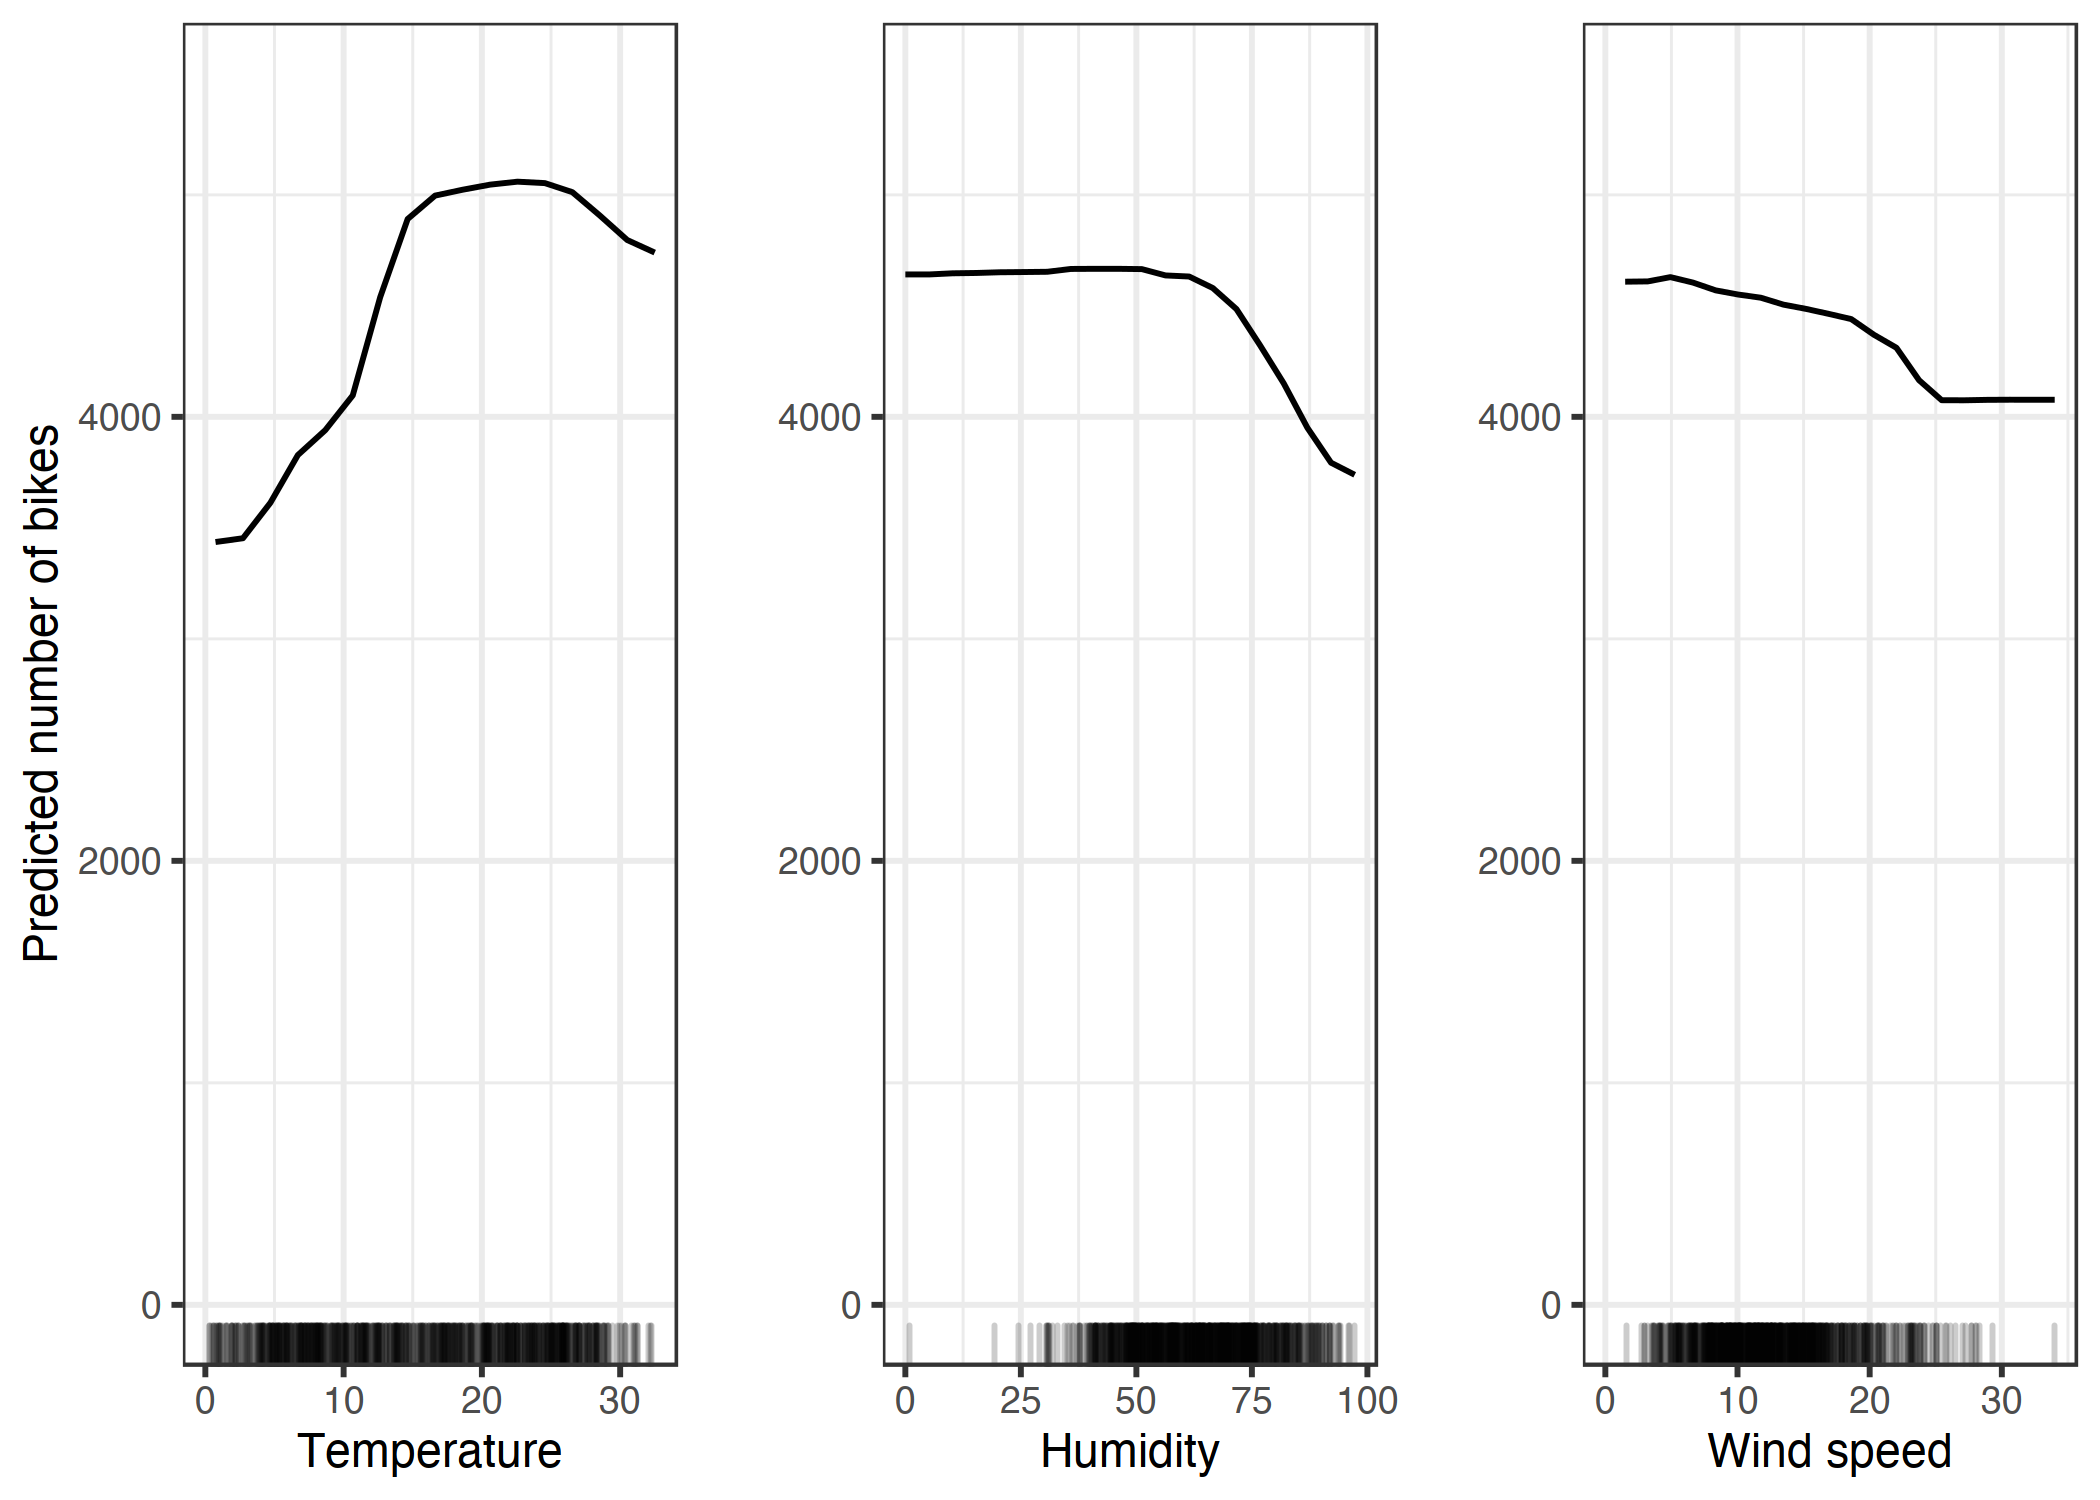
\includegraphics[width=0.7\linewidth]{figure/pdp-bike-1} 

}

\caption[Exemple de graphique de dépendance partielle des variables]{Exemple de graphiques de dépendance partielle des variables extrait de (\protect\hyperlink{ref-molnar_interpretable_2019}{Molnar, 2019}). Le modèle statistique sous-jacent prédit un nombre de vélos loués en fonction d'un ensemble de paramètres météorologiques et socio-économiques. Le graphique montre que la relation capturée par le modèle entre le nombre de vélos prédits et respectivement la température (à gauche), l'humidité (au milieu) et la vitesse du vent (à droite) est non-linéaire}\label{fig:example-pdp}
\end{figure}
Au delà de ces deux exemples, il existe une myriade d'outils d'interprétation à postériori des modèles statistiques (\protect\hyperlink{ref-molnar_interpretable_2019}{Molnar, 2019}) ; et le secteur est en plein développement avec l'intérêt croissant pour l'interprétation des modèles non-paramétriques (\protect\hyperlink{ref-murdoch_definitions_2019}{Murdoch et al., 2019}). Ces outils permettent d'interpréter un modèle ayant potentiellement capturé des relations complexes et non-hypothétisées, et donc d'étudier le comportement du sytème complexe sous toutes ses formes : contribution absolue et relative de ses différentes composantes, relations fonctionnelles, importance et effets des interactions, etc. Ces problématiques sont, typiquement, celles en jeu dans l'étude des systèmes biologiques (\protect\hyperlink{ref-yu_study_2021}{Yu et al., 2021}).\\

Notons enfin que, au même titre que les modèles statistiques, chaque outil d'interprétation possède un lot d'hypothèses d'utilisation et de limites, et qu'il est ainsi important de bien en comprendre le fonctionnement intrinsèque afin de l'utiliser à bon escient et d'en extraire de l'information et de la connaissance pertinente (\protect\hyperlink{ref-molnar_interpretable_2019}{Molnar, 2019}; \protect\hyperlink{ref-zhao_causal_2021}{Zhao \& Hastie, 2021}).

\hypertarget{notes-conclusives}{%
\section{Notes conclusives}\label{notes-conclusives}}

Un modèle statistique est un outil permettant d'associer des données, à savoir des informations mesurables du monde qui nous entoure. Associer des données peut servir différents enjeux scientifiques : tester une théorie scientifique (expliquer), mieux comprendre un phénomène d'intérêt (décrire), prédire de nouvelles valeurs d'un évènement (prédire). Selon l'enjeu, l'ensemble du processus de modélisation statistique diffère : pour un même système étudié, le ``meilleur'' modèle explicatif sera différent du ``meilleur'' modèle prédictif, lui-même différent du ``meilleur'' modèle descriptif (\protect\hyperlink{ref-shmueli_explain_2010}{Shmueli, 2010}).\\

Les premiers modèles statistiques, historiquement, servent principalement l'approche hypothético-déductive de la génération de connaissance scientifique - à savoir, tester une théorie scientifique. Aujourd'hui, l'avènement des données volumineuses, des méthodes statistiques non-paramétriques (qui sont en capacité de ``trouver'' de manière autonome des associations complexes entre variables, parfois difficilement hypothétisables) et des outils permettant d'interpréter les associations capturées par ces modèles, offrent des perspectives nouvelles pour mieux prédire, mais aussi comprendre, les systèmes complexes tels que le système vectoriel. Afin d'exploiter la puissance de la modélisation statistique - c'est à dire, exploiter pleinement son potentiel, sans pour autant le surévaluer (\protect\hyperlink{ref-holzinger_general_2022}{Molnar et al., 2022}) - il est essentiel de maitriser les fondements mêmes de la génération de connaissance scientifique, et de connaitre les étapes du processus de modélisation statistique ainsi que les outils de science des données qui existent.

\begingroup 
\renewcommand{\headrulewidth}{0pt}

\markboth{}{}


\includepdf[pages=2,nup=1,pagecommand={}]{pagesgarde.pdf}
\endgroup

\hypertarget{data-collection-preparation}{%
\chapter{Zones d'étude et préparation des données environnementales télédétectées}\label{data-collection-preparation}}

Les travaux à suivre s'inscrivent dans le cadre d'un projet plus large, nommé REACT ; et ont conduit à la production de nombreuses données. Dans ce chapitre, nous présentons dans un premier temps les objectifs du projet REACT et les deux zones d'études du projet et de la thèse. Dans un second temps, nous décrivons les travaux de génération des données utilisées pour les études présentées dans les chapitres suivants. Enfin, nous apportons quelques précisions sur les logiciels informatiques utilisés pour manipuler les données (recueil, génération, préparation, modélisation) dans le cadre de la thèse, et présentons rapidement les codes informatiques développés pour les besoins de ces travaux.

\hypertarget{study-areas}{%
\section{Présentation du projet REACT et des zones d'études de la thèse}\label{study-areas}}

Les travaux de cette thèse s'inscrivent dans le cadre du projet \emph{REACT : Gestion de la résistance aux insecticides au Burkina Faso et en Côte d'Ivoire : recherche sur les stratégies de lutte anti-vectorielle}, mené en partenariat entre l'Institut de Recherche pour le Développement (IRD, France), l'Institut de Recherche en Sciences de la Santé (IRSS, Burkina Faso) et l'Institut Pierre Richet (IPR, Côte d'Ivoire). Ce projet était financé par L'Initiative 5\%. L'objectif principal de ce projet, dont la phase de terrain s'est déroulée entre les années 2016 et 2018, était d'évaluer l'impact de l'utilisation de mesures de lutte anti-vectorielles complémentaires à la MIILDA sur la transmission et l'épidémiologie du paludisme à travers un essai randomisé contrôlé (ERC). A cette fin, deux zones d'études ont été séléctionnées dans deux pays d'Afrique de l'ouest : le Burkina Faso (BF) et la Côte d'Ivoire (CI).\\

Ces deux pays sont situés en zone endémiques du paludisme à \emph{P. falciparum}. Les courbes épidémiologiques des deux pays (morbidité et mortalité) suivent les tendances observées à l'échelle du continent (cf.~figure \ref{fig:malaria-african-trends}). En 2019, avant la pandémie de covid-19, le nombre de cas de paludisme était estimé à 5,9 millions au Burkina Faso et autant en Côte d'Ivoire (\protect\hyperlink{ref-who_2021}{WHO, 2021}). Comme introduit dans le chapitre 1, les principales espèces d'anophèles dans ces pays sont \emph{An. arabiensis}, \emph{An. gambiae s.s.}, \emph{An. coluzzii} et \emph{An. funestus}; et dans les deux pays les résistances physiologiques des anophèles aux insecticides y sont reportées depuis plusieurs décennies (voir figure \ref{fig:dev-res-phy}).\\

Chaque zone d'étude du projet REACT couvre environ la surface d'un district sanitaire (\textasciitilde2500 km²). Il s'agit de zones principalement rurales. Pour le projet REACT, un total de 55 villages (27 au Burkina Faso, 28 en Côte d'Ivoire) a été séléctionné au sein de ces zones pour mener l'ERC selon les critères suivants : accessibilité pendant la saison des pluies, 200 à 500 habitants par village, et distance entre les villages supérieure à 2 km. La figure \ref{fig:study-areas} présente la localisation géographique des zones et des villages séléctionnés ; ainsi que le chronogramme de collectes de données effectuées dans le cadre du projet REACT.
\begin{figure}

{\centering 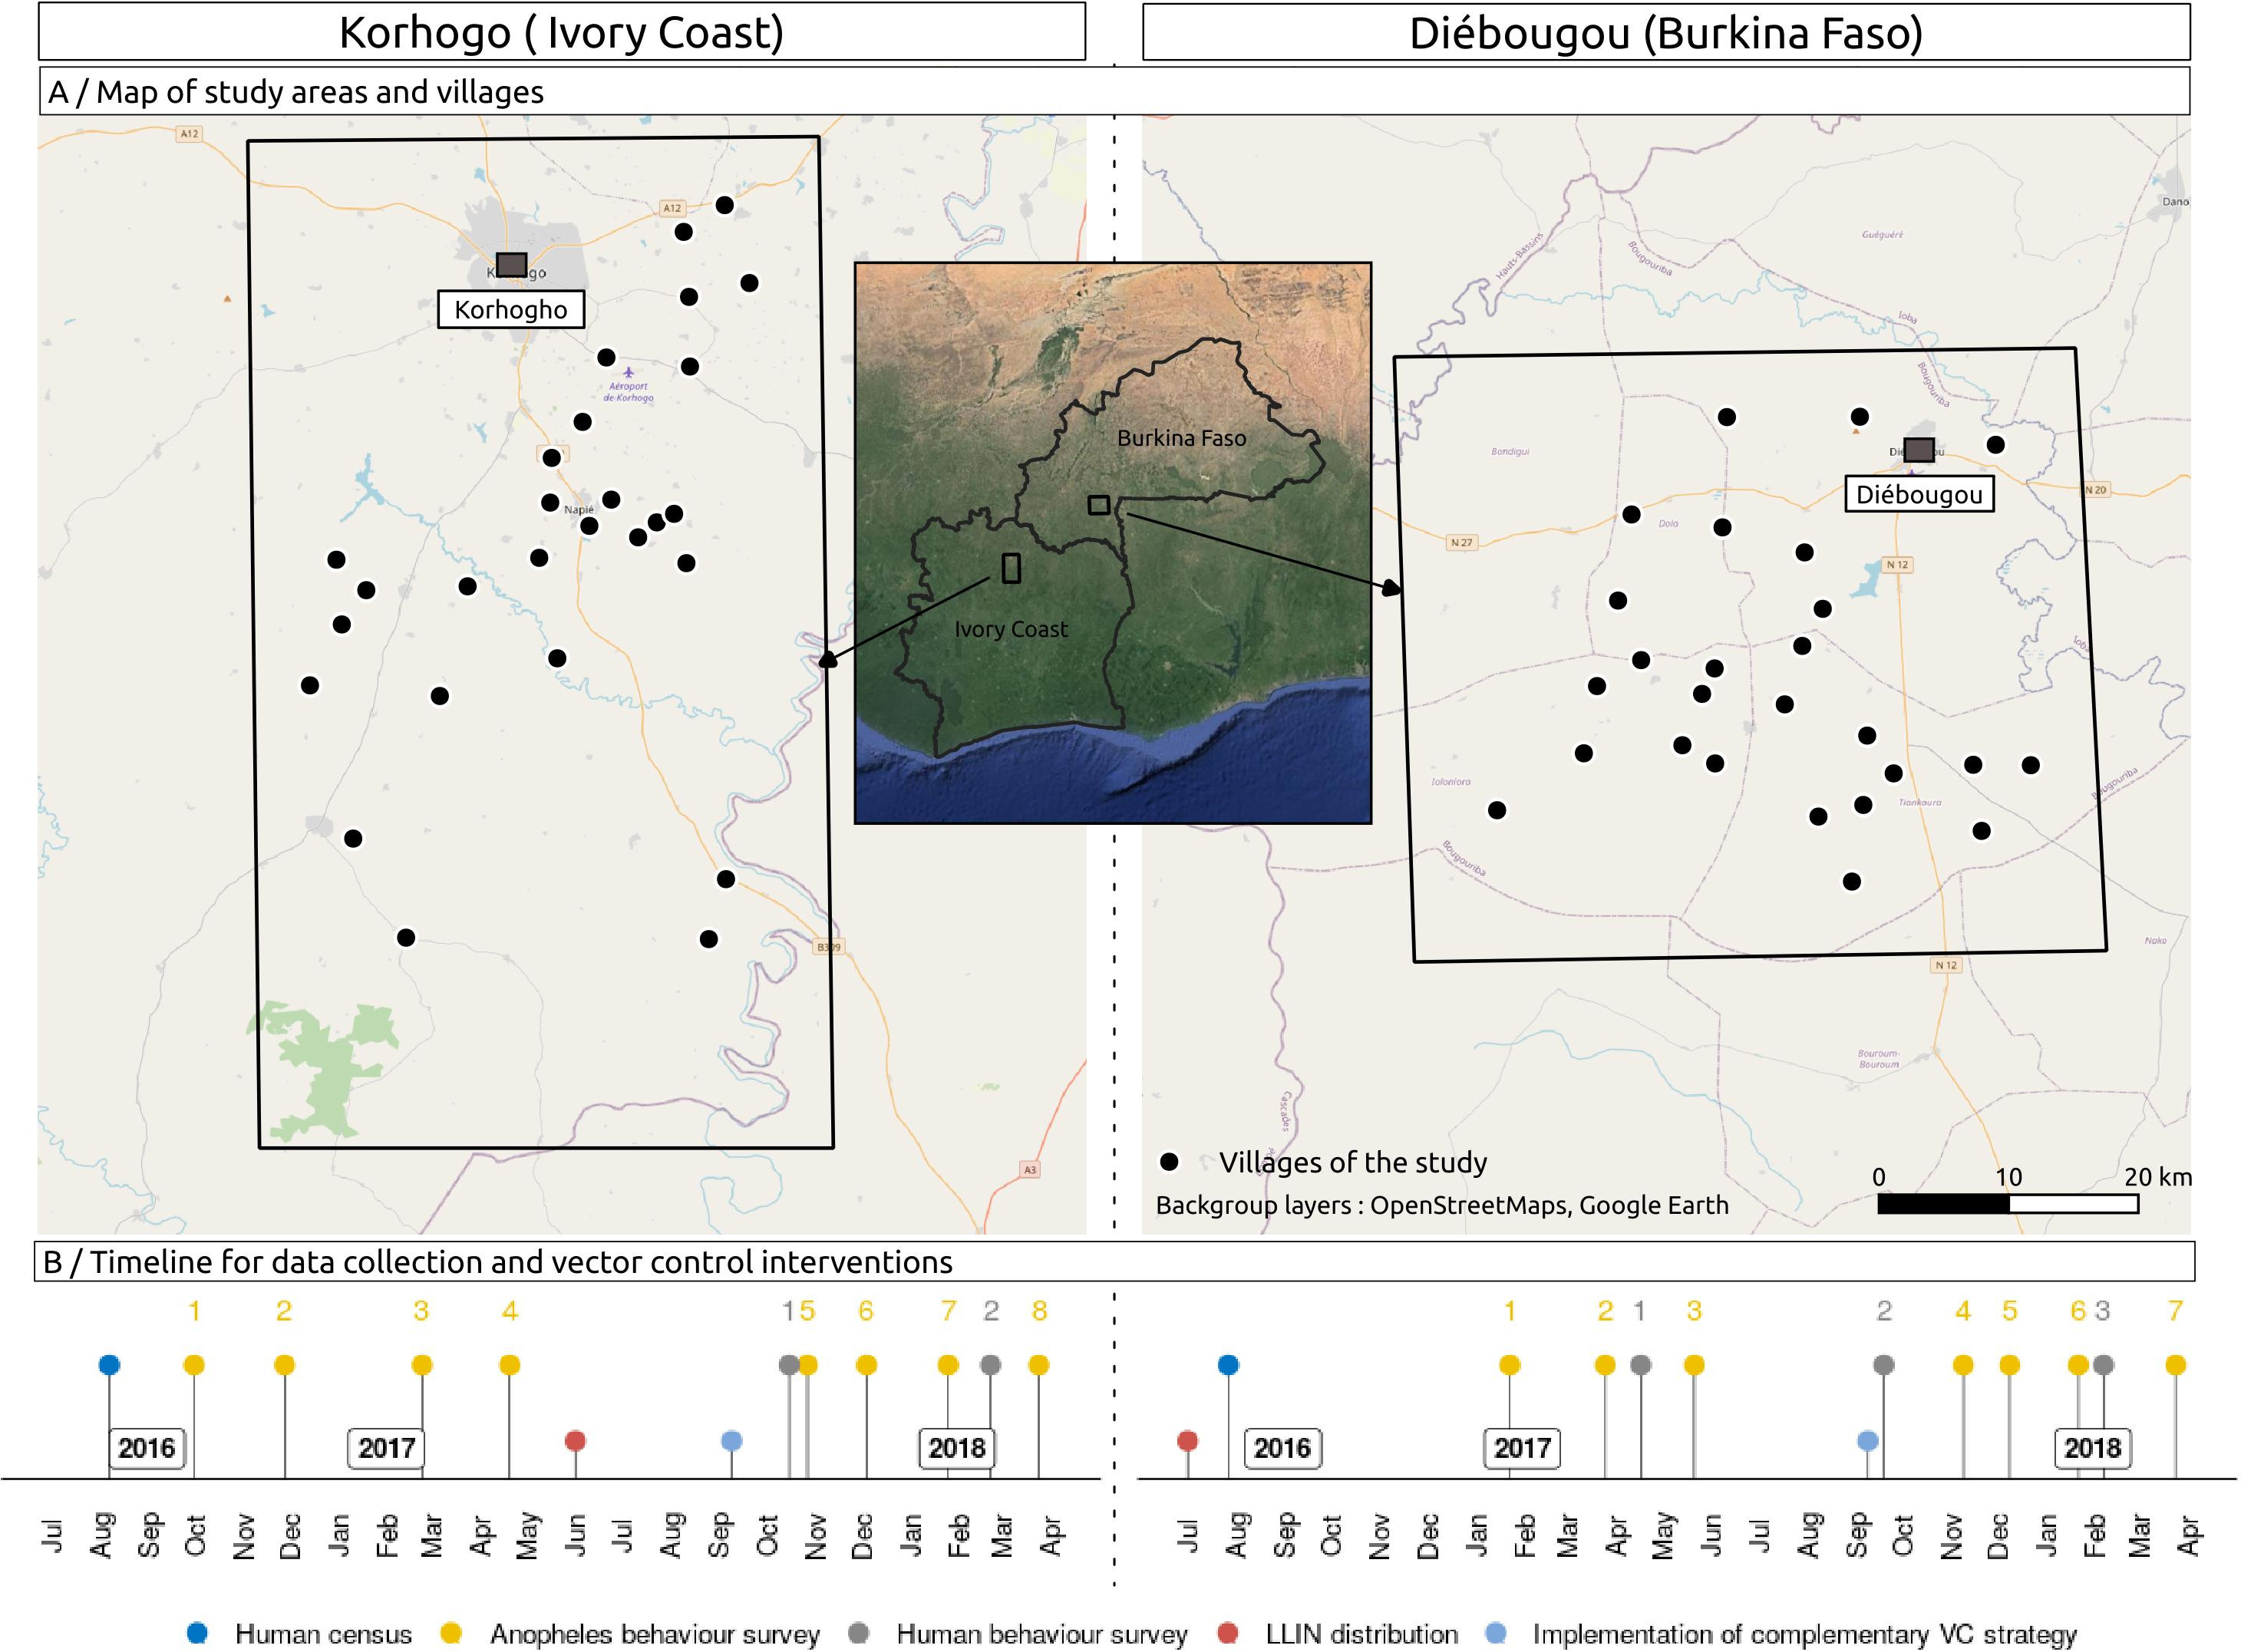
\includegraphics[width=1\linewidth]{figure/carte_zones_react} 

}

\caption[Zones d'étude et villages du projet REACT]{Projet REACT : zones d'étude, villages et dates de collectes des données}\label{fig:study-areas}
\end{figure}
La zone d'étude burkinabé du projet REACT couvre la région de Diébougou, au sud-ouest du pays, en région bioclimatique soudanienne (\protect\hyperlink{ref-cilss_2016_landscapes_nodate}{CILSS, 2016}). Le climat y est caractérisé par une saison sèche d'octobre à avril (incluant une période `froide' de décembre à février et une période `chaude' de mars à avril) et une saison pluvieuse de mai à septembre. Les amplitudes thermiques moyennes journalières sont 18-36 °C, 25-39 °C et 23-33 °C respectivement en saison sèche froide, sèche chaude et pluvieuse. Les précipitations annuelles moyennes sont de 1200 mm. Comme nous allons le voir à la section \ref{landcover-data}, la végétation naturelle est dominée par la savane arborée parsemée de forêts ripicoles. La principale activité économique est l'agriculture (culture des céréales) suivie par l'exploitation artisanale de l'or et la production de charbon et de bois (\protect\hyperlink{ref-INSD_1}{INSD, 2015}, \protect\hyperlink{ref-INSD_2}{2017}). Le principal outil de lutte anti-vectorielle dans la région de Diébougou est la MIILDA, distribuée universellement par le gouvernement tous les 3-4 ans depuis 2010 (\protect\hyperlink{ref-PNLP_BF}{PNLP, 2014a}). La dernière distribution avant le projet REACT datait de juillet 2016 (\protect\hyperlink{ref-PNLP_BF}{PNLP, 2014a}), soit 6 mois avant la première mission de collecte de données entomologiques (voir ci-dessous).\\

La zone d'étude ivoirienne du projet REACT couvre la région de Korhogo, au nord du pays, elle aussi en région bioclimatique soudanienne (\protect\hyperlink{ref-cilss_2016_landscapes_nodate}{CILSS, 2016}). La saisonalité de la climatologie y est relativement similaire à celle de Diébougou (voir section \ref{meteo-data}). Les précipitations annuelles varient de 1200 à 1400 mm, tandis que la température moyenne annuelle varie de 21 à 35 °C. La végétation naturelle est principalement un mélange de savane et de forêt ouverte (voir section \ref{landcover-data}). La région possède une forte densité de barrages hydrauliques qui permettent de pratiquer l'agriculture tout au long de l'année. Comme pour la région de Diébougou, la principale activité économique est l'agriculture (riz, maïs, coton). De même, Le principal outil de lutte anti-vectorielle est là aussi la MIILDA, distribuée universellement par le gouvernement, comme au Burkina Faso, tous les 3-4 ans depuis 2010 (\protect\hyperlink{ref-PNLP_CI}{PNLP, 2014b}). La dernière distribution avant le projet REACT datait de 2014.\\

L'essai randomisé s'est déroulé en 3 phases. La phase pré-intervention a duré environ un an et a principalement consisté à i) établir un recensement exhaustif de la population et de la localisation géographique des ménages dans les villages, ii) recueillir des données entomologiques, épidémiologiques et de comportement humain dans ces villages, iii) distribuer des MIILDA dans les villages d'étude en Côte d'Ivoire (au Burkina Faso, une distribution universelle de moustiquaires a eu lieu en juillet 2016). Environ une année après le début du projet, la phase d'intervention a consisté à implémenter les mesures de LAV complémentaires à la MIILDA (détaillées ci-après) dans certains villages, tirés au sort dans le cadre de l'essai randomisé contrôlé. Enfin, en phase post-intervention (environ 1 an), plusieurs sessions de collecte de données ont été menées selon les mêmes protocoles qu'en phase de pré-intervention. Ainsi, en comparant les données entomologiques et épidémiologiques de pré-intervention et de post-intervention, il est possible de mesurer l'impact des mesures de lutte anti-vectorielles complémentaires à la MIILDA sur la transmission (taux d'inoculation entomologique) et l'épidémiologie (prévalence et incidence) du paludisme.\\
\begin{lightcyanbox}
\begin{center}
Boite info n°4 : \textbf{Mesures complémentaires de LAV déployées dans le cadre du projet REACT}

\end{center}
Les mesures complémentaires de lutte anti-vectorielle déployées dans le cadre du projet REACT étaient les suivantes :
\begin{itemize}
\tightlist
\item
  \textbf{Information, Education, Communication (IEC)} (testée dans les zones BF et CI). A travers des activités de sensibilisation des populations, l'objectif de cette intervention etait d'optimiser la mise en place des MILDA, l'adhésion des populations aux campagnes de lutte et l'utilisation correcte et régulière des MIILDA.
\item
  \textbf{Pulvérisations intra-domiciliaires} (PID) de Pirimiphos-méthyle (Actellic) appliquées sur les murs des habitations (testées dans les zones BF et CI). En complément des MIILDA qui visent les vecteurs endophages uniquement, l'objectif des PID etait de tuer les vecteurs endophiles qui auraient résisté à l'insecticide utilisé dans les moustiquaires.
\item
  \textbf{Lutte anti-larvaire} (\protect\hyperlink{ref-djenontin_field_2014}{Djènontin et al., 2014}) (testée dans la zone CI uniquement). Cette intervention visait à diminuer la population générale de vecteurs, en tuant les moustiques à leur état larvaire par l'utilisation d'insecticides d'origine bactérienne.
\item
  \textbf{Administration d'ivermectine} aux hôtes (testée dans la zone BF uniquement). L'ivermectine est une molécule administrée aux hôtes pour lutter contre les endoparasites. Elle diminue la longévité d'un moustique ayant pris un repas sanguin sur un hôte traité (\protect\hyperlink{ref-alout_evaluation_2014}{Alout et al., 2014}; \protect\hyperlink{ref-ouedraogo_efficacy_2015}{Ouedraogo et al., 2015}). Dans le projet REACT, l'ivermectine a été administrée aux populations animales péri-domestiques dans le but de cibler les populations de vecteurs présentant des comportements zoophages ou opportunistes.
\end{itemize}
\end{lightcyanbox}
\hfill\break

Les travaux de thèse à suivre utilisent en grande partie des jeux de données recueillies sur le terrain dans le cadre du projet REACT, en particulier :
\begin{itemize}
\tightlist
\item
  les données \textbf{entomologiques},
\item
  les données de \textbf{recensement des villages} (population, localisation des habitations),
\item
  un jeu de données \textbf{environnementales et climatiques au cours des collectes entomologiques},
\item
  un jeu de données de \textbf{comportement humain} relatives à l'utilisation des MIILDA et aux habitudes horaires de sommeil.
\end{itemize}
Les données entomologiques constituent la source des variables à expliquer / prédire dans les travaux de modélisation, tandis que les autres données ont été utilisées pour caractériser l'environnement à proximité spatiale et temporelle des points de capture des vecteurs (variables explicatives / prédictives). Les protocoles de recueil de ces données sont détaillés dans les études qui les utilisent, ainsi qu'à l'annexe \ref{data-terrain} de ce manuscrit.\\

Les conditions météorologiques (températures, précipitations) et paysagères (utilisation, occupation du sol) peuvent impacter l'abondance, le comportement, ou les résistances des vecteurs (voir les introductions des articles des chapitres 4 et 5 pour davantage de détails), objets d'étude de travaux de la thèse. Aussi, nous avons complété les données recueillies sur le terrain avec trois autres jeux de données environnementales, générées pour les deux zones d'étude :
\begin{itemize}
\tightlist
\item
  données \textbf{météorologiques} au cours des semaines précédant les collectes entomologiques,
\item
  données d'\textbf{occupation et utilisation des sols},
\item
  données sur le \textbf{réseau hydrographique théorique}.
\end{itemize}
Ces données environnementales ont été générées à partir de produits satellitaires d'observation de la Terre. En effet, les satellites sont en mesure de capturer de nombreux paramètres environnementaux en surface ou dans l'atmosphère terrestre. Les capteurs embarqués sur ces satellites mesurent le rayonnement électromagnétique réfléchi ou émis par la surface terrestre, les océans ou l'atmosphère. Ces données brutes peuvent ensuite être traitées pour en extraire des informations environnementales telles que les précipitations, les températures au sol, l'altitude ou encore l'occupation du sol. Ces données sont particulièrement intéressantes et précieuses pour caractériser l'environnement dans des zones où les observatoires ou stations météorologiques au sol sont rares, telles que les zones rurales ouest-africaines. Aussi, les images satellitaires sont très largement utilisées en géo-épidémiologie, pour expliquer ou prédire des indicateurs entomologiques ou épidémiologiques (\protect\hyperlink{ref-ebhuoma_remote_2016}{Ebhuoma \& Gebreslasie, 2016}; \protect\hyperlink{ref-parselia_satellite_2019}{Parselia et al., 2019}). Dans la suite de ce chapitre, nous détaillons les traitements qu'il a été nécessaire de réaliser pour produire ou exploiter ces données en vue des travaux de modélisation à suivre dans les prochains chapitres.

\hypertarget{production-des-donnuxe9es-environnementales-tuxe9luxe9duxe9tuxe9ctuxe9es}{%
\section{Production des données environnementales télédétéctées}\label{production-des-donnuxe9es-environnementales-tuxe9luxe9duxe9tuxe9ctuxe9es}}

\hypertarget{meteo-data}{%
\subsection{Données de météorologie}\label{meteo-data}}

Nous avons extrait les températures et les précipitations dans nos zones d'études sur les périodes précédant les collectes entomologiques à partir de produits satellitaires d'observation de la Terre. Pour les précipitations, nous avons utilisé les produits de la mission \emph{Global Precipitation Measurement} (GPM) (voir point info ci-dessous). Pour les températures, nous avons utilisé les données recueillies par l'instrument \emph{Moderate Resolution Imaging Spectroradiometer} (MODIS) embarqué à bord des satellites Terra et Aqua. En particulier, nous avons utilisé les collections GPM et MODIS suivantes :
\begin{itemize}
\tightlist
\item
  \emph{MOD11A1.006} (\protect\hyperlink{ref-wan__zhengming_mod11a1_2015}{Wan, Hook, \& Hulley, 2015a}) : Températures de surface terrestre diurnes et nocturnes extraites de l'instrument MODIS embarqué sur le satellite Terra (résolution spatiale : 1 km, résolution temporelle : 1 jour)
\item
  \emph{MYD11A1.006} (\protect\hyperlink{ref-wan__zhengming_myd11a1_2015}{Wan, Hook, \& Hulley, 2015b}) : Températures de surface terrestre diurnes et nocturnes extraites de l'instrument MODIS embarqué sur le satellite Aqua (résolution spatiale : 1 km, résolution temporelle : 1 jour)
\item
  \emph{GPM\_3IMERGDF.06} (\protect\hyperlink{ref-nasa_goddard_earth_sciences_data_and_information_services_center_gpm_2019}{NASA, 2019}) : Précipitations extraites de GPM (résolution spatiale : 0.1 ° (\textasciitilde{} 10 km), résolution temporelle : 1 jour)\\
\end{itemize}
\begin{lightcyanbox}
\begin{center}
Boite info n°5 : \textbf{GPM et MODIS : des données météorologiques à l'échelle mondiale et à fine résolution spatio-temporelle}

\end{center}
Initiée par la NASA et la JAXA (agences spatiales respectivement états-uniennes et japonaises), la mission GPM est un projet international en cours depuis l'année 2014, comprenant une constellation de satellites appartenant à plusieurs agences spatiales nationales. À sa résolution spatio-temporelle la plus fine, elle fournit des estimations des précipitations à une résolution de 10 km / 30 minutes pour l'ensemble du globe en temps quasi réel (4 heures de latence entre l'acquisition du satellite et la mise à disposition des données). Les estimations sont ensuite consolidées via divers algorithmes de correction, pour créer des produits consolidés destinés à la recherche environ 3 mois après l'acquisition. Les données GPM sont générées à différentes résolutions temporelles (30 minutes, 1 jour, 1 mois). Tous les produits sont gratuits et libres d'accès pour l'utilisateur.\\

L'instrument MODIS est embarqué à bord de Terra et Aqua de la NASA, deux satellites d'observation de la Terre lancés respectivement en 1999 et 2002. Les différents spectromètres de MODIS prennent une image complète de la Terre tous les 1 à 2 jours. Les satellites Terra et Aqua fonctionnant en phase et l'instrument MODIS capturant des données strictement identiques, les produits MODIS issus des deux satellites peuvent être combinés pour obtenir des produits à résolution temporelle très fine (jusqu'à 0.5 jour). Les observations brutes de MODIS sont traitées automatiquement par différents algorithmes de la NASA pour générer des produits dits de ``haut niveau'', directement utilisables par les différentes communautés scientifiques (océanographie, biologie, sciences de l'atmosphère, etc.). Les produits de haut niveau de MODIS comprennent, par exemple, la réflectance de la surface, la température de surface de la terre et de la mer, la couverture neigeuse, la concentration de chlorophylle-a dans l'océan, des indices de végétation, etc. Les résolutions spatiales et temporelles varient en fonction du produit. Toutes les données MODIS sont ouvertes et gratuites, et mises à disposition des utilisateurs finaux à différentes échéances temporelles après l'acquisition (quelques heures à une année, en fonction du produit).\\

\end{lightcyanbox}
Nous avons choisi d'extraire ces données de précipitations et températures sur une période de six semaines (soit 42 jours) précédant chaque collecte entomologique. Cette période permet en effet de couvrir largement la durée de vie d'un anophèle sur le terrain (incluant les phases aquatiques et larvaires) (\protect\hyperlink{ref-holstein_biologie_1952}{Holstein, 1952}). La quantité de données à extraire (3 collections de produits satellitaires, 2 zones d'études, plusieurs centaines de dates d'intérêt) nous a emmené à nous poser la question de la méthode à utiliser pour ce faire. Les données MODIS et GPM sont originellement stockées sur les serveurs de la NASA. Afin de s'adapter aux différents besoins, habitudes et compétences techniques des utilisateurs finaux des produits satellitaires, l'agence met à disposition de multiples outils pour les télécharger et les propose dans de nombreux formats numériques. Parmi les différents outils disponibles pour accéder aux données, un a particulièrement retenu notre attention : le protocole OPeNDAP.\\
\begin{lightcyanbox}
\begin{center}
Boite info n°6 : \textbf{Le protocole OPeNDAP}

\end{center}
OPeNDAP est l'acronyme de ``Open-source Project for a Network Data Access Protocol'', un projet (et le nom du serveur) visant à faciliter l'accès à des données structurées (telles que les produits satellitaires) sur le Web. L'une des principales forces d'OPeNDAP est qu'il permet de filter les produits satellitaires dès la phase de téléchargement - spatialement, temporellement et dimensionnellement. Ainsi, seule la partie réellement utile des données pour l'utilisateur est téléchargée (et le volume de données téléchargées est donc limité au strict nécéssaire) ; ce qui contraste avec la plupart des interfaces `clic-bouton' d'accès aux données - où de grands volumes de données sont généralement importés, quand bien même l'utilisateur n'en nécéssiterait qu'une petite partie. Notons aussi que le projet OPeNDAP est développé collaborativement par plusieurs institutions et entreprises, que le code source et ouvert et que le logiciel est gratuit.\\

Pour télécharger un produit satellitaire disponible sur un serveur OPeNDAP, il s'agit d'envoyer au serveur une URL dans laquelle les filtres (spatiaux, temporels, dimensionnels) sont spécifiés. Par exemple l'URL suivante :

\url{https://opendap.cr.usgs.gov/opendap/hyrax/MOD11A1.006/h17v08.ncml.nc4?MODIS_Grid_Daily_1km_LST_eos_cf_projection,LST_Day_1km} {[}6093:6122{]}{[}55:140{]}{[}512:560{]},LST\_Night\_1km{[}6093:6122{]}{[}55:140{]}{[}512:560{]} ,time{[}6093:6122{]},YDim{[}55:140{]},XDim{[}512:560{]}

permet de télécharger les bandes LST\_Day\_1km et LST\_Night\_1km (filtre dimensionnel) du produit MOD11A1.006 entre le 1er et le 30 janvier 2017 (filtre temporel) sur la zone délimitée par les coordonnées géographiques suivantes (en WGS84) : xmin: -5.82 ymin: 8.84 xmax: -5.41 ymax: 9.55 (coordonnées de la zone CI du projet REACT).

\end{lightcyanbox}
La pluspart des données d'observation de la Terre produites par la NASA sont disponibles en accès OPeNDAP, mais utiliser ce protocole pour télécharger des données reste compliqué pour l'utilisateur néophyte (en particulier, la constitution de l'URL n'est pas triviale, comme le montre l'exemple précédent). Afin de faciliter l'extraction de ces données depuis les serveurs OPeNDAP, nous avons développé une librairie dans le langage de programmation R (\protect\hyperlink{ref-r_core_team_r_2018}{R Core Team, 2018}) que nous avons nommée \href{https://github.com/ptaconet/opendapr}{\textbf{opendapr}}. La principale fonction de cette librairie, nommée \texttt{odr\_get\_url}, prend en argument une collection d'intérêt (par exemple \texttt{MOD11A1.006}), une période d'intérêt (sous forme d'une date de début et de fin), une aire géographique d'intérêt (sous forme des coordonnées géographiques qui la délimitent), et des bandes d'intérêts (par exemple \texttt{LST\_Night\_1km}), et contruit automatiquement l'URL qui permettra finalement de télécharger le produit satellitaire d'intérêt. Une seconde fonction, \texttt{odr\_download\_data}, permet ensuite de télécharger le produit en local. À ce jour, la librairie permet de télécharger 77 collections de produits satellitaires recueillis sur toute la surface terrestre (incluant les produits MODIS et GPM, mais aussi SMAP (humidité du sol) et VIIRS (successeur de MODIS)). Au delà de son utilisation pour les travaux de cette thèse, cette librairie présente l'intérêt de rendre l'accès à certains produits satellitaires plus aisé aux utilisateurs de R, en particulier si la connexion à internet de l'utilisateur est lente et/ou onéreuse, de promouvoir une forme de sobriété digitale dans les travaux de recherche scientifique, et de soutenir le mouvement des logiciels libres et ouverts (sur lesquels nous nous sommes exclusivement basés pour l'ensemble de nos travaux, cf.~section \ref{software}).\\

La libraire est disponible à l'adresse suivante : \url{https://github.com/ptaconet/opendapr}, et une description plus détaillée de la librairie est disponible en annexe \ref{annex-opendapr} de ce manuscrit.\\

Une fois les produits téléchargés localement, nous avons préparé les données dans l'objectif de constituer des variables statistiques exploitables dans des modèles. Nous avons rééchantillonné les produits GPM (précipitations) depuis leur résolution spatiale initiale (10 km) à une résolution d'un kilomètre, en utilisant une méthode d'interpolation bilinéaire. Nous avons également combiné les produits journaliers MODIS issus de Terra et Aqua, en conservant les valeurs de pixels les plus élevées (respectivement les plus basses) disponibles pour les températures diurnes (respectivement nocturnes). Nous avons finalement comblé les valeurs manquantes dans les pixels (principalement dues à la présence de nuages) en interpolant temporellement les valeurs disponibles aux dates les plus proches.\\

La figure \ref{fig:plot-pastweather} montre les séries temporelles hebdomadaires des précipitations et températures sur les deux zones d'études, extraites des données GPM et MODIS LST. Le bandeau gris représente la variabilité spatiale autour des différents points de captures entomologiques. L'alternance des saisons sèches et pluvieuses dans les deux zones d'études est clairement visible sur les graphiques de précipitations. Notons que les températures diurnes sont plus élevées dans la zone de Diébougou que dans celle de Korhogo, que les températures nocturnes sont relativement similaires, et que les précipitations en saison pluvieuse sont plus abondantes à Korhogo qu'à Diébougou.
\begin{figure}

{\centering 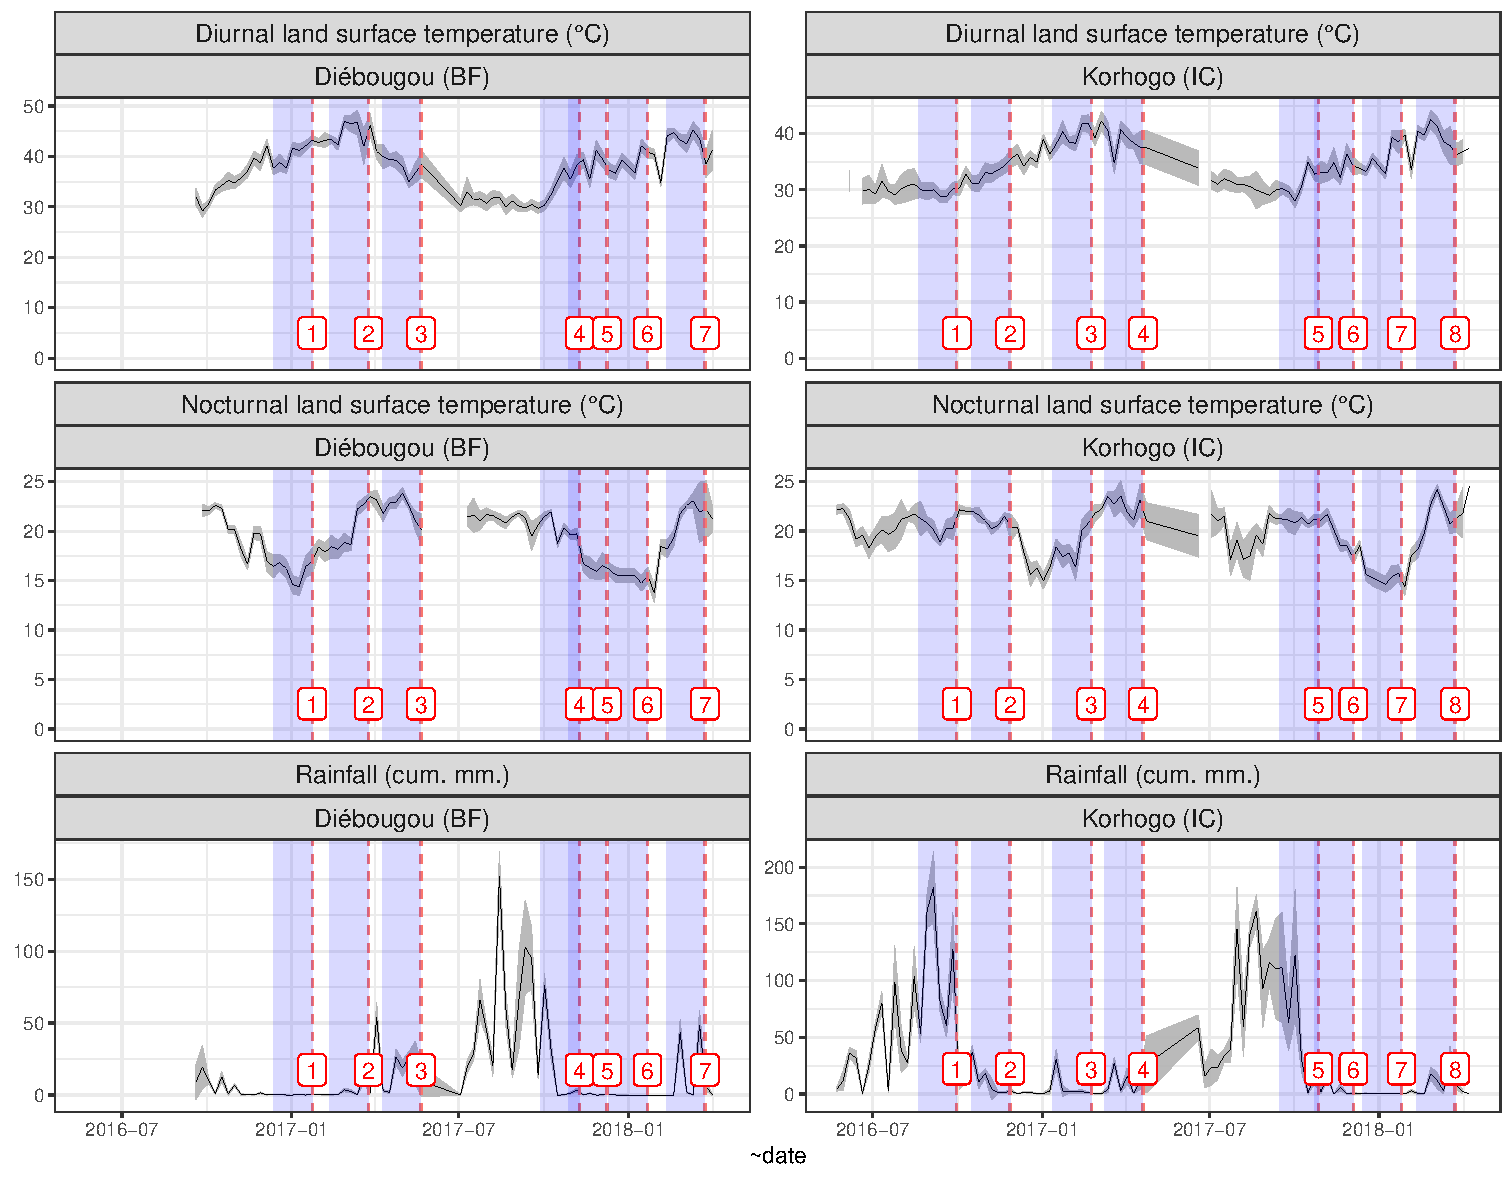
\includegraphics[width=1\linewidth]{figure/plot_pastweather} 

}

\caption[Courbes des conditions météorologiques sur les deux zones d'étude]{Courbes des conditions météorologiques sur les deux zones d'étude. Les lignes noires indiquent la moyenne de la variables météorologique pour tous les points de collectes entomologiques pour la semaine considérée.
 Les bandeaux gris indiquent la moyenne ± l'écart type (i.e. la variabilité spatiale pour la semaine considérée).
 Les lignes rouges verticales indiquent les dates des collectes entomologiques.
Les bandeaux bleus indiquent une période de six semaines précédant chaque collecte entomologique.
Source des données : GPM (précipitations), MODIS (températures diurnes et nocturnes)}\label{fig:plot-pastweather}
\end{figure}
\hypertarget{landcover-data}{%
\subsection{Données d'occupation du sol}\label{landcover-data}}

La caractérisation de l'occupation des sols sur un territoire peut être obtenue par classification d'images satellitaires (\protect\hyperlink{ref-anderson_land_1976}{Anderson, Hardy, Roach, \& Witmer, 1976}) ou aériennes (\protect\hyperlink{ref-horning_mapping_2020}{Horning, Fleishman, Ersts, Fogarty, \& Wohlfeil Zillig, 2020}). Nous avons ainsi cartographié l'occupation du sol sur nos deux zones d'étude à l'aide d'une classification supervisée orientée objet de produits satellitaires d'observation de la Terre (\protect\hyperlink{ref-blaschke_geographic_2008}{G. J. Hay \& Castilla, 2008}).\\
\begin{lightcyanbox}
\begin{center}
Boite info n°7 : \textbf{Concept et principales étapes d'une classification supervisée orientée objet de produits satellitaires d'observation de la Terre}

\end{center}
Le principe de la cartographie de l'occupation du sol par télédétection spatiale est d'attribuer une classe d'occupation du sol à chaque pixel ou groupe de pixel d'une (ou plusieurs) image(s) géoréférencée(s). On peut distinguer deux grandes approches de classification d'images satellitaires à des fins de cartographie d'occupation du sol : i) l'approche orientée `pixel', où chaque pixel de l'image satellitaire ou aérienne est classé individuellement sans tenir compte des pixels adjacents, et ii) l'approche orientée `objet' (\protect\hyperlink{ref-blaschke_geographic_2008}{G. J. Hay \& Castilla, 2008}), où les pixels adjacents ayant des propriétés communes sont d'abord regroupés en `objets', ces objets étant ensuite classés. L'approche orientée objet est particulièrement adaptée dans les cas où la résolution spatiale des pixels de l'image est largement inférieure à celle des entités constituant les classes d'occupation du sol que l'on cherche à extraire (\protect\hyperlink{ref-blaschke_geographic_2008}{G. J. Hay \& Castilla, 2008}) : par exemple, si la résolution du pixel est de quelques (centi)mètres mais que l'on cherche à extraire des informations type `zones forestières'. Par ailleurs, l'approche orientée objet permet la classification non plus seulement sur les seules valeurs spectrales des pixels mais sur un ensemble de caractéristiques associées à l'objet : forme, relation avec les objets voisins, statistique sur les valeurs des pixels qui le compose, etc. Le qualificatif `supervisé' fait référence, en modélisation statistique, au caractère connu \emph{à priori} des classes (ici, d'occupation du sol) que l'on souhaite obtenir, par opposition à la classification non-supervisée où les classes sont automatiquement définies par un algorithme.\\

Les principales étapes d'une classification supervisée orientée objet sont les suivantes (\protect\hyperlink{ref-blaschke_geographic_2008}{G. J. Hay \& Castilla, 2008}) :
\begin{enumerate}
\def\labelenumi{\arabic{enumi}.}
\tightlist
\item
  \emph{Acquisition des produits satellitaires} : Il s'agit tout d'abord d'acquérir le(s) produit(s) satellitaire(s) qui sera(ont) utilisé(s) pour la classification. Notons que plusieurs produits satellitaires peuvent être utilisés, afin d'augmenter le volume et la diversité des informations capturées - et ainsi en théorie la qualité de la classification. Par exemple, il est possible d'utiliser une ou plusieurs images satellitaires optiques - qui donneront des informations sur la réfléctance des objets au sol dans plusieurs bandes spectrales - et un modèle numérique de terrain - qui donnera des informations sur le relief (altitude, pente, etc.).
\item
  \emph{Constitution du jeu de données d'apprentissage et de validation} : Dans le cas d'une classification supervisée, il est nécessaire de constituer un jeu de donnée d'apprentissage / validation composé de plusieurs échantillons (parcelles) géoréférencés de chaque classe d'occupation du sol présentes dans la zone d'étude (les `vérités terrain'). Ce travail nécessite donc i) de définir la liste des classes d'occupation du sol potentiellement présentes sur le territoire d'intérêt ; et ii) de constituer le jeu de données d'apprentissage / validation, par des enquêtes sur le terrain ou par photo-interprétation.
\item
  \emph{Prétraitements des produits satellitaires} : Le ou les produits satellitaires utilisés pour la classification peuvent nécessiter un ensemble de prétraitements, selon leur degré de `préparation' à l'étape d'acquisition. Parmi les prétraitements classiques, citons par exemple : la fusion des tuiles (dans le cas où la zone d'étude est composée de plusieurs tuiles satellitaires), la calibration optique (conversion des pixels dans le cas où les images satellitaires optiques ne sont pas prises sous les mêmes conditions atmosphériques), le traitement des pixels indisponibles (par exemple, à cause de la couverture nuageuse), ou encore l'orthorectification (afin d'améliorer le géoréférencement des images).
\item
  \emph{Segmentation} : Cette étape est celle de la constitution des `objets' par regroupement des pixels adjacents ayant des propriétés communes. Il existe plusieurs algorithmes de segmentation. Une des méthodes pour définir des objets consiste à agréger les pixels de proche en proche jusqu'à atteindre des seuils d'hétérogénéités fixés par l'utilisateur (liés à la taille des objets, à leurs formes, et aux valeurs contenues dans les pixels), interrompant le processus et délimitant l'objet (\protect\hyperlink{ref-baatz_schape_2000}{Baatz \& Schape, 2000}).
\item
  \emph{Constitution des variables prédictives} : Il s'agit ensuite de calculer pour chaque objet un ensemble d'attribut qui servira à entraîner le modèle sur le jeu d'entrainement, et à prédire sur les objets issus de la segmentation. Ces variables prédictives peuvent être basées sur des descripteurs statistiques des valeurs des pixels qui composent l'objet, sur la forme de l'objet, sa relation avec les objets voisins, etc.
\item
  \emph{Classification} : Vient ensuite l'étape de la classification même : un modèle prédictif est d'abord entraîné sur les parcelles du jeu d'entraînement, puis est utilisé pour prédire la classe d'occupation du sol sur l'ensemble des objets de la zone d'étude.
\item
  \emph{Evaluation de la qualité de la classification} : Enfin, la qualité de la classification est évaluée en prédisant l'occupation du sol sur le jeu de données de validation, puis en générant la matrice de confusion et les métriques de performances classiques afférentes (indices kappa, \emph{accuracy}, etc.)
\end{enumerate}
\end{lightcyanbox}
\hfill\break

Dans notre cas, le détail des traitements ayant permis de génerer les produits d'occupation du sol à partir de classifications supervisées orientées objets de produits satellitaires est présenté ci-après.\\

\textbf{\emph{1. Acquisition des produits satellitaires}}. Nous avons aquis les produits satellitaires suivants sur chaque zone d'étude :
\begin{itemize}
\tightlist
\item
  \emph{images SPOT 6 et 7} (Satellite Pour l'Observation de la Terre) : images optiques à Très Haute Résolution Spatiale (THRS). Dates d'aquisition par le(s) satellite(s) : octobre 2017. Résolution spatiale : 1.6 m en panchromatique et 6.3 m en multispectral. Nombre de bandes spectrales : 4. Ces images ont été commandées via le dispositif Geosud, un projet (ANR-10-EQPX-20) du programme ``Investissements d'Avenir'' géré par le Centre National de la Recherche Scientifique.
\item
  \emph{images Sentinel-2} : images optiques à Haute Résolution Spatiale (HRS). Dates d'aquisition par le(s) satellite(s) : novembre / décembre 2018 (corresponsant aux dates des campagnes d'acquisition de vérités terrain, voir ci-dessous). Résolution spatiale : 10 m à 60 m selon les bandes. Nombre de bandes spectrales : 10. Ces images libres d'accès ont été téléchargées sur le portail Copernicus SciHub de l'Agence spatiale européenne. L'intérêt d'utiliser des images Sentinel-2 en complément des images SPOT 6/7 est double : i) diversifier la nature et augmenter le nombre des variables prédictives (les images Sentinel-2 contiennent une information spectrale plus riche que les images SPOT-6 (10 bandes contre 4 bandes), et ii) intégrer des images acquises simultanément aux campagnes d'acquisition des vérités terrain.
\item
  \emph{Shuttle Radar Topography Mission (SRTM)} (\protect\hyperlink{ref-nasa_jpl_nasa_2013}{JPL, 2013}) : Modèle Numérique de Terrain (MNT) procurant la valeur de l'altitude en tout point du globe. Résolution spatiale : 30 m. Ce MNT libre d'accès a até téléchargé sur portail EarthExplorer (\url{https://earthexplorer.usgs.gov/}).
\end{itemize}
\textbf{\emph{2. Constitution du jeu de données d'apprentissage et de validation}}. Nous avons mené une campagne d'acquisition de vérités terrain sur chacune des zones en novembre et décembre 2018 (10 jours sur la zone burkinabé, 14 jours sur la zone ivoirienne). Nous avons établi les classes d'occupation du sol dans chacune des zones sur la base de recherches bibliographiques sur les types de paysages potentiellement rencontrés dans nos zones (\protect\hyperlink{ref-aubreville_accord_1957}{Aubréville, 1957}; \protect\hyperlink{ref-cilss_2016_landscapes_nodate}{CILSS, 2016}; \protect\hyperlink{ref-oss_landcover_bf}{OSS, 2015}) et de nos observations du paysage sur le terrain. Nous avons collecté un minimum de 20 parcelles par classe, en tentant de les répartir au mieux sur l'étendue de chacune des zones. Sur le terrain, nous avons collecté les données à l'aide de l'application QField, compatible avec le logiciel de Système d'Information Géographique QGIS (\protect\hyperlink{ref-qgis_development_team_qgis_2021}{QGIS Development Team, 2021}). Nous avons ensuite complété le jeu de données en y ajoutant quelques parcelles par photo-interprétation d'images satellitaires très haute résolution (Google Earth et Spot 6/7).\\

\textbf{\emph{3. Prétraitements des produits satellitaires}}. Les images SPOT ont été préparées selon la suite d'opérations suivante : fusion des tuiles de l'image panchromatique (PAN); conversion des images panchromatiques et multispectrales (MS) en valeurs de réflectance `Top-of-Atmosphere'; orthorectification des images PAN et MS en utilisant les informations disponibles dans les métadonnées des fichiers ainsi que le MNT SRTM (dont la résolution spatiale est suffisante pour une orthorectification de qualité au regard du profil de nos zones, peu accidentées); découpage des images sur l'étendue de nos zones d'études uniquement; `pansharpening' de l'image MS utilisant l'image PAN; mosaïquage des images (uniquement dans le cas de la zone de Diébougou, qui était constituée de deux images SPOT). Les produits Sentinel 2 et SRTM, de leur côté, ont nécéssité relativement peu de prétraitements. Nous avons reprojeté le MNT originellement fourni en WGS84 sur la zone UTM 30 Nord (zone UTM correspondant à nos zones d'étude), mosaiqué les images (dans le cas où nos zones d'études étaient couvertes par plusieurs tuiles) et découpé les produits afin de les conserver uniquement sur l'étendue de nos zones d'études.\\

\textbf{\emph{4. Segmentation}}. Nous avons ensuite segmenté les images SPOT en utilisant un algorithme de croissance de région avec le critère d'homogénéité de Baatz and Shape (\protect\hyperlink{ref-baatz_schape_2000}{Baatz \& Schape, 2000}). Nous avons testé plusieurs paramétrisations, à la fois de l'algorithme (paramètres d'échelle, spectraux et de compacité) et des bandes spectrales utilisées pour la segmentation (bandes spectrales de l'image SPOT pan-sharpenées, bandes spectrales + indices spectraux type NDVI, etc.). Basé sur une approche visuelle des résultats de la segmentation (en les superposant à l'image SPOT 6/7), nous avons finalement retenu les paramètres suivants :
\begin{itemize}
\tightlist
\item
  Bandes spectrales utilisées pour la segmentation : les 4 bandes spectrales de l'image SPOT 6/7 pan-sharpenée, chacune avec un poids égal dans la segmentation ;
\item
  Paramètres de segmentation pour la zone de Diébougou (BF) : seuil = 100 ; valeur pour le poids de forme = 0.1 ; valeur pour le poids spectral = 0.9
\item
  Paramètres de segmentation pour la zone de Korhogo (CI) : seuil = 160 ; valeur pour le poids de forme = 0.1 ; valeur pour le poids spectral = 0.8
\end{itemize}
Nous avons vectorisé le jeu de données en sortie de l'algorithme afin d'avoir une version vecteur des objets segmentés. Puis, nous avons intersecté la base de données d'apprentissage (parcelles d'occupation du sol recueillies sur le terrain) avec la couche résultant de la segmentation, dans l'objectif d'obtenir des parcelles d'apprentissage plus homogènes du point de vue des critères de segmentation. Cette étape a sensiblement fait croître le nombre de parcelles d'entraînement - les objets issus de la segmentation étant globalement plus fragmentés et petits que les parcelles relevées sur le terrain. C'est cette couche de données d'apprentissage qui sera utilisée pour la suite du travail.\\

\textbf{\emph{5. Constitution des variables prédictives}}. Afin de générer les variables prédictives, nous avons extrait ou calculé les couches géographiques suivantes (sous forme de fichiers raster) :
\begin{itemize}
\tightlist
\item
  Couches issues de l'image SPOT 6/7 :
  \begin{itemize}
  \tightlist
  \item
    chacune des 4 bandes spectrales de la THRS pan-sharpenée ;
  \item
    image panchromatique ;
  \item
    indices spectraux suivants: NDVI, NDWI2, BRI ;
  \item
    indices de texture suivants, extraits de l'image PAN : energie, anthropie, correlation, inertie, haralick correlation, moyenne. Chacun des indices a été calculé sur 3 tailles de fenêtres glissantes : 5 pixels, 9 pixels, 17 pixels ;
  \end{itemize}
\item
  Couches issus de l'image Sentinel-2 :
  \begin{itemize}
  \tightlist
  \item
    chacune des 10 bandes spectrales ;
  \item
    indices spectraux suivants : NDVI, NDWI, BRI, MNDWI, MNDVI, RNDVI (ces trois derniers indices sont des variantes des indices classiques NDWI et NDVI qui utilisent les bandes spectrales dans le moyen infra-rouge) ;
  \end{itemize}
\item
  Couches issues du MNT SRTM :
  \begin{itemize}
  \tightlist
  \item
    altitude ;
  \item
    pente ;
  \item
    réseau hydrographique théorique (couche vectorielle).
  \end{itemize}
\end{itemize}
Au total, cela représentait ainsi 45 couches géographiques utilisables pour générer les variables prédictives. Nous avons calculé la moyenne et l'écart type des valeurs des pixels pour l'ensemble des indices préparées pour la classification sur chaque objet. Nous avons également calculé et ajouté les descripteurs contextuels suivants : i) la distance de chaque objet au réseau hydrographique théorique (calculé à partir du MNT, voir section \ref{hydro-data}), et ii) un ensemble d'indices liés à la forme des objets (aire, périmètre, etc.). La centaine de variables ainsi générée constituait les prédicteurs pour la classification à suivre.\\

\textbf{\emph{6. Classification}}. Nous avons ensuite entrainé un modèle de forêts aléatoires sur le jeu de données d'entrainement. Nous avons généré la matrice de confusion en utilisant la procédure de validation interne aux forêts aléatoires (basée sur les `out-of-bag' observations (\protect\hyperlink{ref-Breiman1996OUTOFBAGE}{Breiman, 1996})). En se basant sur cette matrice, nous avons ensuite regroupé, dans le jeu de données d'entrainement, les classes d'occupation du sol dont la confusion était importante (par exemple, zones de culture de mil et de sorgho) ; en prenant cependant soin de conserver la distinction entre les différentes classes à priori favorables à la présence de gîtes larvaires (par exemple, zones marécageuses et rizicoles) ou à la résistance. Nous avons entrainé un modèle de forêt aléatoires sur cette nouvelle version du jeu de données d'entraînement puis l'avons utilisé pour prédire la classe d'occupation du sol sur chaque objet issu de la segmentation.\\

\textbf{\emph{7. Evaluation de la qualité de la classification}}. Comme précédemment, nous avons généré la matrice de confusion puis en avons extrait un indice de qualité de la classification (\emph{accuracy} (\protect\hyperlink{ref-cohen_coefficient_1960}{J. Cohen, 1960})) mesurant la proportion d'objets correctement classés.\\

Les différentes étapes de la classification sont résumées graphiquement dans la figure \ref{fig:workflow-obia} disponible en annexe \ref{details-annex-landcover}. Nous avons développé un script R implémentant l'ensemble des traitements (voir section \ref{scripts}).\\

Le tableau \ref{tab:table-landcover} présente les classes d'occupation du sol initialement définies et finalement retenues. La définition de chacune des classes ainsi qu'un ensemble de photographies représentatives des principales classes d'occupation du sol, prises lors des campagnes de terrain, sont disponibles en annexe \ref{annex-landcover}.

\pagebreak
\begin{table}[!h]

\caption[Classes d'occupation du sol initialement définies et finalement retenues]{\label{tab:table-landcover}Classes d'occupation du sol initialement définies et finalement retenues}
\centering
\fontsize{8}{10}\selectfont
\begin{tabular}[t]{>{\bfseries}lll}
\toprule
Classes retenues & Classes initialement définies & Présence sur zone(s) d’étude\\
\midrule
 & Eau dormante & BF et CI\\
\cmidrule{2-3}
\multirow[t]{-2}{*}{\raggedright\arraybackslash \makecell[l]{Eau permanente \\(Permanent water bodies)}} & Eau courante & BF et CI\\
\cmidrule{1-3}
 & À maïs & BF et CI\\
\cmidrule{2-3}
 & À poids de terre & BF et CI\\
\cmidrule{2-3}
 & À arachide & BF et CI\\
\cmidrule{2-3}
 & À mil & BF\\
\cmidrule{2-3}
 & À sorgho & BF\\
\cmidrule{2-3}
 & À haricot & BF\\
\cmidrule{2-3}
 & À sésame & BF\\
\cmidrule{2-3}
\multirow[t]{-8}{*}{\raggedright\arraybackslash \makecell[l]{Culture et jachère, hors coton et riz \\(Crops)}} & Jachère & CI\\
\cmidrule{1-3}
\makecell[l]{Culture cotonière \\(Cotton)} & Culture cotonière & BF et CI\\
\cmidrule{1-3}
\makecell[l]{Rizière \\(Rice)} & Rizière & BF et CI\\
\cmidrule{1-3}
 & À mangue & CI\\
\cmidrule{2-3}
\multirow[t]{-2}{*}{\raggedright\arraybackslash \makecell[l]{Plantation \\(Plantation)}} & À anacarde & CI\\
\cmidrule{1-3}
 & Savane arbustive & BF\\
\cmidrule{2-3}
 & Savane arborée & BF\\
\cmidrule{2-3}
 & Savane boisée & BF\\
\cmidrule{2-3}
\multirow[t]{-4}{*}{\raggedright\arraybackslash \makecell[l]{Savane ligneuse \\(Ligneous savannah)}} & Savane dégradée & CI\\
\cmidrule{1-3}
\makecell[l]{Prairie \\(Grassland)} & Prairie & BF\\
\cmidrule{1-3}
 & Forêt dense & CI\\
\cmidrule{2-3}
\multirow[t]{-2}{*}{\raggedright\arraybackslash \makecell[l]{Milieu forestier non humide \\(Woodland)}} & Forêt claire & BF et CI\\
\cmidrule{1-3}
\makecell[l]{Forêt ripicole \\(Riparian forest)} & Forêt ripicole & BF et CI\\
\cmidrule{1-3}
\makecell[l]{Prairie marécageuse \\(Marsh)} & Prairie marécageuse & BF et CI\\
\cmidrule{1-3}
\makecell[l]{Bâti \\(Settlements)} & Bâti & BF et CI\\
\cmidrule{1-3}
\makecell[l]{Sol nu \\(Bare soil)} & Sol nu & BF et CI\\
\cmidrule{1-3}
\makecell[l]{Route principale \\(Main tracks)} & Routes principales & BF et CI\\
\bottomrule
\end{tabular}
\end{table}
\pagebreak

Les matrices de confusion indiquaient que respectivement 84 \% et 86 \% des objets dans les zones de Diébougou et Korhogo étaient bien classés. Les cartes \ref{fig:map-landcover-bf} et \ref{fig:map-landcover-ci} présentent les produits finis d'occupation du sol dans les deux zones d'étude. Ces cartes incluent également le réseau hydrographique théorique, généré à partir du MNT SRTM (voir section \ref{hydro-data}).
\begin{figure}

{\centering 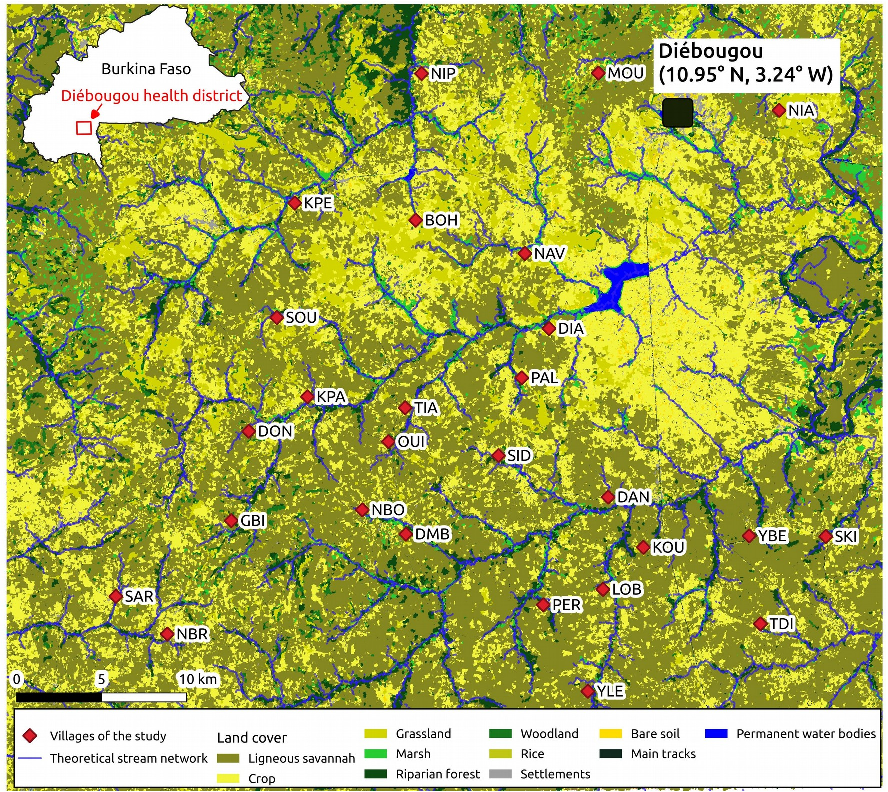
\includegraphics[width=1\linewidth]{figure/map_landcover_bf} 

}

\caption[Carte d'occupation du sol résultante des travaux de classification dans la zone de Diébougou (BF)]{Carte d'occupation du sol résultante des travaux de classification dans la zone de Diébougou (BF) (résolution spatiale : 1,5 x 1,5 m)}\label{fig:map-landcover-bf}
\end{figure}
\pagebreak
\begin{figure}

{\centering 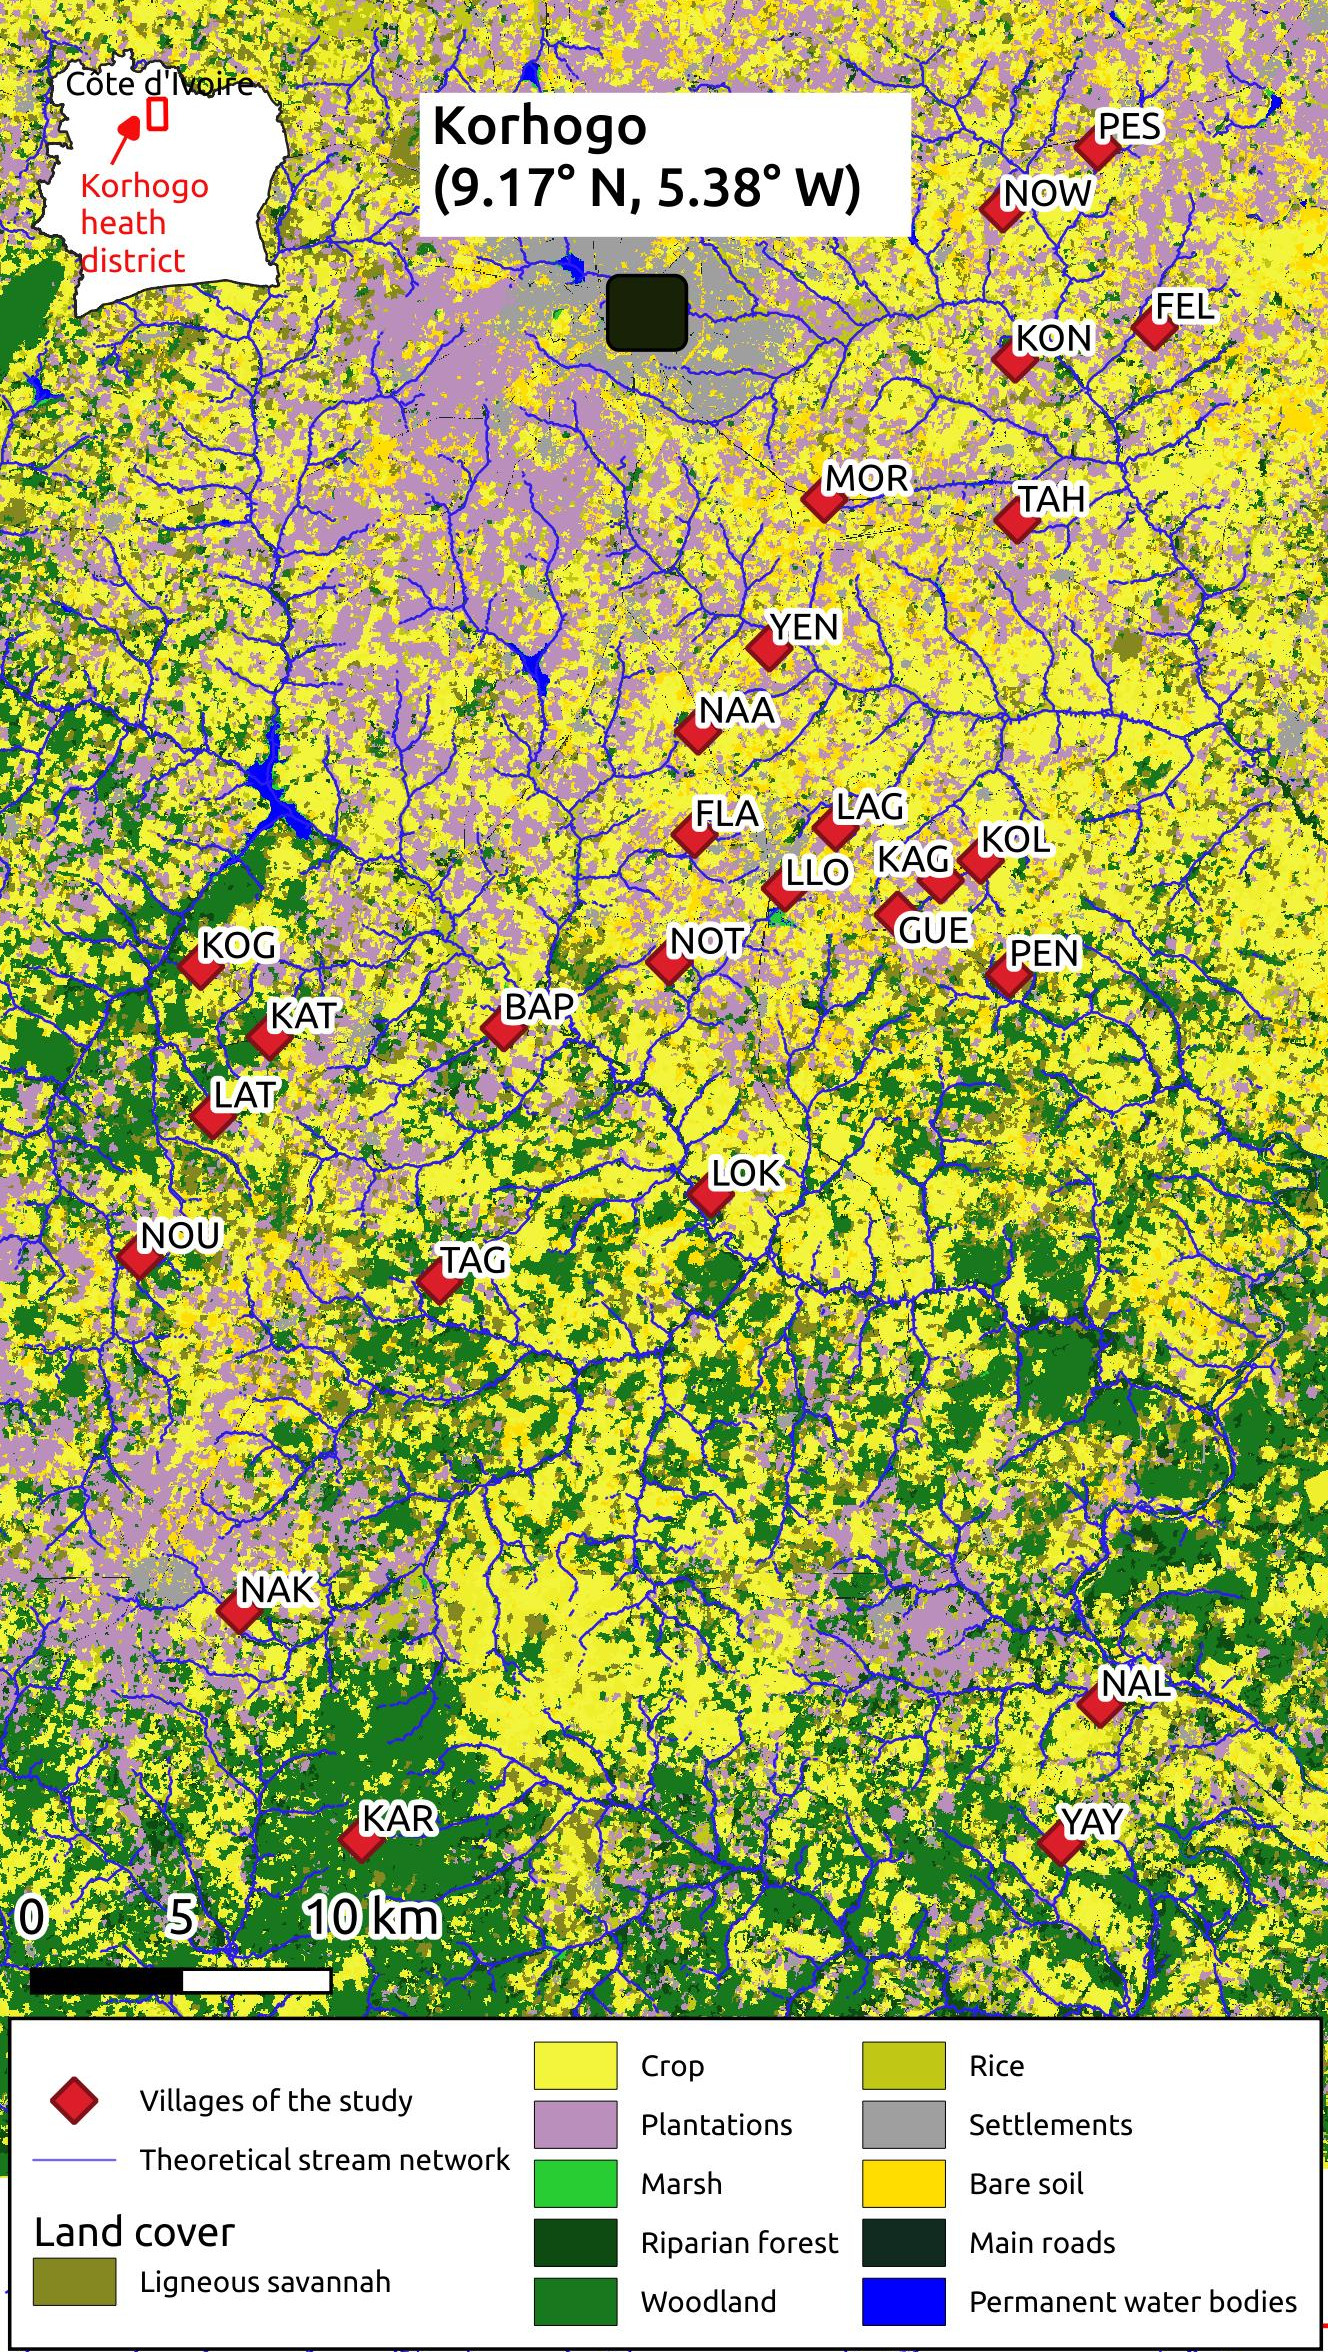
\includegraphics[width=0.8\linewidth]{figure/map_landcover_ci} 

}

\caption[Carte d'occupation du sol résultante des travaux de classification dans la zone de Korhogo (CI)]{Carte d'occupation du sol résultante des travaux de classification dans la zone de Korhogo (CI) (résolution spatiale : 1,5 x 1,5 m)}\label{fig:map-landcover-ci}
\end{figure}
\pagebreak

Enfin, la figure \ref{fig:landcover-stats} présente la proportion de surface occupé par chaque classe d'occupation du sol dans l'ensemble de la zone d'étude.
\begin{figure}

{\centering 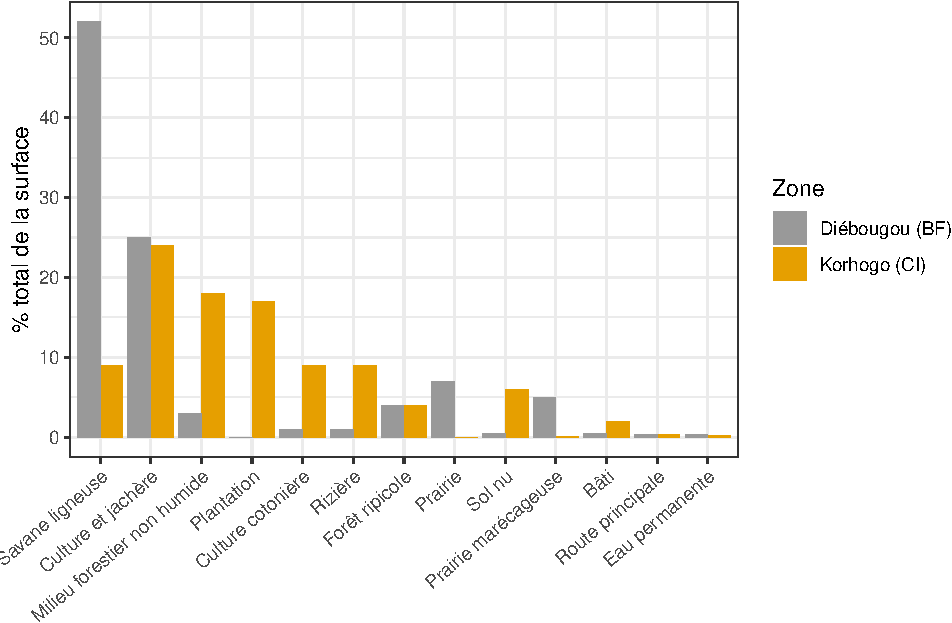
\includegraphics[width=1\linewidth]{these_taconet_files/figure-latex/landcover-stats-1} 

}

\caption[Proportion de surface occupée par chaque classe d'occupation du sol sur chaque zone d'étude]{Proportion de surface occupée par chaque classe d'occupation du sol sur chaque zone d'étude}\label{fig:landcover-stats}
\end{figure}
Nous pouvons noter que la zone de Diébougou était dominée par les savanes ligneuses (52\% de la surface totale), les cultures non-inondées (25\%) et les prairies non-inondées (7\%). La zone de Korhogo, de son côté, était principalement composée de cultures non-inondées (24\%), de milieux forestiers non-humides (18\%) et de plantations d'anacardiers et mangues (17\%). Les rizicultures et cultures de coton y représentaient chacune 9\% de la surface totale.

\hypertarget{hydro-data}{%
\subsection{Données sur le réseau hydrographique théorique}\label{hydro-data}}

Le réseau hydrographique (cad. les rivières) est susceptible de produire des gîtes larvaires pour les anophèles. Nous avons utilisé le MNT SRTM pour produire le réseau hydrographique théorique dans nos zones d'étude. Nous avons tout d'abord produit une couche raster d'accumulation de flux à partir du MNT (\protect\hyperlink{ref-jenson_extracting_1988}{Jenson \& Domingue, 1988}), puis avons sélectionné tous les pixels dont la valeur d'accumulation de flux était supérieur à un seuil défini visuellement par superposition avec une image satellite THRS. Ces seuils étaient de 1000 pour la zone BF et 800 pour la zone CI. Les réseaux hydrographiques théoriques sont représentés sur les cartes \ref{fig:map-landcover-bf} et \ref{fig:map-landcover-ci}.

\hypertarget{ressources-informatiques-codes-r-duxe9veloppuxe9s-et-logiciels-utilisuxe9s}{%
\section{Ressources informatiques : codes R développés et logiciels utilisés}\label{ressources-informatiques-codes-r-duxe9veloppuxe9s-et-logiciels-utilisuxe9s}}

\hypertarget{scripts}{%
\subsection{Codes R développés}\label{scripts}}

L'ensemble des travaux d'extraction et préparation des données décrits dans ce chapitre a été programmé, sous formes de codes informatiques, dans le language de programmation R (\protect\hyperlink{ref-r_core_team_r_2018}{R Core Team, 2018}) sous l'environnement RStudio (\protect\hyperlink{ref-rstudio_team_rstudio_2020}{RStudio Team, 2020}). Les travaux de modélisation de l'ensemble des articles à suivre ont eux aussi été scriptés en R.\\

Le niveau de description, généricité, réutilisation diffère selon les codes. Le plus abouti en ce sens est la librairie \texttt{opendapr}, puisqu'il s'agit d'une réelle libraire R. D'une manière générale, les codes de création, extraction et préparation des données ont un niveau acceptable de description et généricité (à savoir, ils peuvent être réutilisés tout ou partie à moindre coût par un utilisateur de R). Les codes de modélisation statistique sont moins décrits et reproductibles. Quel que soit le niveau de généricité et description, nous avons archivé l'ensemble de ces codes en leur état à l'issue des travaux de thèse, afin d'en conserver une copie pérenne et conforme aux travaux effectués. Le dossier contenant les codes est disponible à l'adresse suivante : \url{https://doi.org/10.5281/zenodo.6334110} . L'architecture du dossier est décrite dans le tableau \ref{tab:scripts-developed}.

\renewcommand{\arraystretch}{2}
\begin{table}[!h]

\caption[Codes R développés au cours de la thèse]{\label{tab:scripts-developed}Codes R développés au cours de la thèse}
\centering
\fontsize{9}{11}\selectfont
\begin{tabu} to \linewidth {>{\raggedright}X>{\raggedright\arraybackslash}p{12cm}}
\toprule
Nom du dossier & Description du contenu\\
\midrule
\rowcolor{gray!6}  data\_creation extraction\_preparation & Ce dossier contient les codes R développés pour créer, extraire, préparer les données environnementales : \newline \newline             - le sous-dossier data\_creation\_extraction contient les codes pour i) (extraction\_landcover\_data) générer les données d'occupation du sol par classification supervisée orientée objet de produits satellitaires, ii) (extraction\_meteo\_data) extraire les produits météorologiques avec la librairie opendapr, iii) (extraction\_miscellaneous\_data) extraire des données environnementales diverses (les données de magnitude visuelle de la Lune (IMCCE), les données de vent (ERA-5), le MNT SRTM) \newline \newline             - le sous-dossier data\_preparation contient les codes développés pour extraire les données, les préparer, et calculer les variables explicatives pour les travaux de modélisation statistique\\
data\_modeling & Ce dossier contient les codes R développés pour les travaux de modélisation statistique : \newline \newline             - le sous-dossier modeling contient les codes pour générer les modèles statistiques des chapitres 4 et 5 \newline \newline             - le sous-dossier models\_analysis contient les codes pour analyser (interpréter) les modèles statistiques\\
\bottomrule
\end{tabu}
\end{table}
\renewcommand{\arraystretch}{1}

\hypertarget{software}{%
\subsection{Logiciels et librairies utilisés}\label{software}}

Les logiciels et librairies utilisées pour nos travaux de thèse étaient tous libres d'accès et à code source ouvert.\\

Les données d'occupation du sol (section \ref{landcover-data}) et du réseau hydrographique théorique (section \ref{hydro-data}) ont été générés en utilisant les librairies R suivantes : \texttt{RSAGA} (\protect\hyperlink{ref-brenning_rsaga_2018}{Brenning, Bangs, \& Becker, 2018}), \texttt{rgrass7} (\protect\hyperlink{ref-bivand_rgrass7_2018}{Bivand, 2018}), \texttt{raster} (\protect\hyperlink{ref-hijmans_raster_2020}{Hijmans, 2020}), \texttt{sf} (\protect\hyperlink{ref-pebesma_simple_2018}{Pebesma, 2018}), \texttt{rgdal} (\protect\hyperlink{ref-bivand_rgdal_2019}{Bivand, Keitt, \& Rowlingson, 2019}) et \texttt{randomForest} (\protect\hyperlink{ref-liaw_classification_2002}{Liaw \& Wiener, 2002}). Certaines de ces librairies utilisent en arrière-plan les logiciels libres SAGA GIS (\protect\hyperlink{ref-conrad_system_2015}{Conrad et al., 2015}) et GRASS GIS (\protect\hyperlink{ref-GRASS_GIS_software}{GRASS Development Team, 2017}). La segmentation a été réalisée grâce à l'algorithme `Generic Region Merging Segmentation' implémenté dans le logiciel libre Orfeo Toolbox (\protect\hyperlink{ref-grizonnet2017orfeo}{Grizonnet et al., 2017}).\\

Désireux de soutenir le mouvement du logiciel libre, nous avons rédigé au cours de la thèse un tutoriel d'initiation à la télédétéction spatiale (cartographie de l'occupation/utilisation du sol) sur logiciel libre (QGIS (\protect\hyperlink{ref-qgis_development_team_qgis_2021}{QGIS Development Team, 2021}) et SAGA GIS). Le tutoriel est disponible en annexe \ref{formation-teledec}. Nous l'avons utilisé au cours d'une formation en télédétéction dispensée à des étudiants de niveau master.\\

Les travaux de modélisation dans les études qui suivent ont eux aussi nécéssité l'utilisation de nombreuses librairies R, qui sont précisées dans les sections \emph{Matériel et méthode} des articles respectifs.\\

Le logiciel de gestion de la bibliographie utilisé pour cette thèse était Zotero. Enfin, l'ensemble des travaux de thèse a été réalisé sur un ordinateur équipé d'Ubuntu, un système d'exploitation à code source ouvert utilisant le noyau Linux ; et ce manuscrit de thèse a été rédigé en \LaTeX  en s'appuyant sur les librairies R \texttt{rmarkdown} (\protect\hyperlink{ref-markdown}{Allaire, Horner, Xie, Marti, \& Porte, 2019}), \texttt{knitr} (\protect\hyperlink{ref-knitr}{Xie, 2020}), \texttt{bookdown} (\protect\hyperlink{ref-bookdown}{Xie, 2019}), \texttt{thesisdown} (\protect\hyperlink{ref-thesisdown}{Ismay \& Solomon, n.d.}), \texttt{kableExtra} (\protect\hyperlink{ref-kableExtra}{Zhu, 2019}).

\hypertarget{data-mining-abundances}{%
\chapter{Article n°1 - Modélisation des dynamiques spatio-temporelles des abondances des vecteurs}\label{data-mining-abundances}}

Dans cette première étude, nous nous intéressons aux déterminants environnementaux de la présence et de l'abondance des espèces vectrices du paludisme dans nos zones d'étude. Comprendre de quelle manière l'environnement impacte la distribution et la densité des anophèles, et pouvoir prédire ces densités à fine échelle spatio-temporelle, peut en effet aider à concevoir et déployer des interventions de LAV efficaces (voir section \ref{explain-risk}). L'étude présentée dans ce chapitre avait ainsi pour objectif d'affiner les connaissances sur les liens entre environnement et nombre de contacts hommes-vecteurs et d'évaluer la prédictibilité spatio-temporelle des densités agressives, dans nos deux zones d'étude. Pour cela, nous étudions le système \{environnement - abondance des vecteurs\} dans une approche holistico-inductive, avec un processus de modélisation statistique en deux étapes. Nous exploitons pleinement la granularité spatio-temporelle des données environnementales à notre disposition et le potentiel descriptif et prédictif des modèles statistiques non-paramétriques pour expliquer et évaluer la prédictibilité des densités agressives des vecteurs dans nos zones d'étude. Pour la zone de Diébougou (BF), cette étude a fait l'objet d'une publication scientifique en tant qu'auteur principal (\url{https://doi.org/10.1186/s13071-021-04851-x}), que nous résumons puis intégrons dans ce chapitre. Dans une troisième partie (section \ref{repro-article-korhogo}), nous présentons et discutons les résultats dans la zone d'étude de Korhogo (CI).\\

\hypertarget{summary-article-2}{%
\section{Résumé de l'article}\label{summary-article-2}}

Les objectifs principaux de cette étude étaient i) d'approfondir les connaissances sur les déterminants environnementaux (en particulier météorologiques et paysagers) des densités agressives des anophèles dans la zone de Diébougou, et ii) d'évaluer la prédictibilité des densités agressives des anophèles dans l'espace et dans le temps.\\

Nous avons modélisé les densités agressives des vecteurs dans la zone de Diébougou en fonction des conditions météorologiques et paysagères à proximité des points de capture. La variable à expliquer était le nombre de contacts homme-vecteur par homme et par nuit de capture. Nous avons constitué des variables explicatives météorologiques à partir des données de météorologie précédant les collectes entomologiques, des variables paysagères à partir des données d'occupation du sol et du réseau hydrographique théorique, et des variables liées à l'attractivité et la pénétrabilité des habitations à partir des données de localisation des habitations. Les variables paysagères ont été calculées dans des zones tampon de rayon variable autour de chaque point de capture, et les variables météorologiques ont été calculées dans tous les intervalles de temps possibles entre 0 et 6 semaines avant les dates de collecte. Nous avons modélisé les densités agressives des vecteurs en deux étapes, apportant des informations complémentaires sur la bio-écologie des anophèles. Dans un premier temps, nous avons calculé les coefficients de corrélation de Spearman entre l'abondance des vecteurs et chaque variable environnementale prise aux différentes zones tampons (pour les variables paysagères) et intervalles de temps (pour les variables météorologiques) ; dans l'objectif d'identifier les périodes (précédant la capture) et espaces (autour du point de capture) pour/dans lesquels nos variables environnementales influençaient au plus les densités agressives. Dans un second temps, nous avons entraîné puis interprété des modèles multivariés d'apprentissage automatique (fôrets aléatoires) afin d'identifier i) l'importance relative des variables environnementales dans l'abondance des vecteurs et ii) l'effet respectif (relation fonctionnelle) de chaque variable environnementale sur l'abondance des vecteurs. Nous avons également évalué la capacité des modèles multivariés à prédire sur de nouveaux villages, par validation croisée. Pour des raisons à la fois d'ordre statistique et biologique, nous avons modélisé séparément la probabilité de présence des vecteurs (probabilité de contact homme-vecteur) et l'abondance des vecteurs (nombre de contacts homme-vecteurs dans les sessions de capture avec au moins un contact). De plus, nous avons modélisé séparément les trois espèces majeures d'anophèles identifiées sur le terrain (\emph{An. gambiae s.s.}, \emph{An. coluzzii}, \emph{An. funestus}), car les déterminants environnementaux de la présence / abondance de chacune peuvent différer.\\

Nous avons observé que les densités agressives étaient, sans surprise, très hétérogènes dans le temps (entre les saisons) et dans l'espace (entre les villages). Dans l'analyse bivariée (coefficients de corrélation), les variables météorologiques et paysagères étaient souvent statistiquement significativement corrélées avec la présence ou l'abondance des vecteurs ; et les coefficients de corrélation variaient fréquemment selon la distance, spatiale (pour les variables paysagères) ou temporelle (pour les variables climatiques), au point de capture. Dans l'analyse multivariée, de nombreux seuils et associations non-linéaires ont été révélés par les modèles d'apprentissage automatique, tant pour les variables météorologiques que pour les variables du paysage. Les modèles multivariés présentaient de bonnes puissances prédictives, indiquant que dans l'ensemble, les déterminants de l'abondance des vecteurs ont été identifiés.\\

L'interprétation des modèles nous a permis de formuler des hypothèses sur la bioécologie des principales espèces vectrices du paludisme dans la zone de Diébougou. Nous avons conjecturé que les conditions météorologiques (températures, précipitations) affectaient tous les stades de vie des moustiques capturés (larves, adultes) à des niveaux variables selon l'espèce et le paramètre météorologique. La météorologie avait parfois un impact plus important encore sur les périodes précédant la durée de vie de la génération échantillonnée. Des gites larvaires préférentiels pour chaque espèce ont été proposés : \emph{An. funestus}, \emph{An. coluzzii} et \emph{An. gambiae s.s.} semblaient être distribués le long d'un gradient de persistance des sites de reproduction, de permanent à temporaire, confirmant la littérature. Par ailleurs, le niveau d'ouverture du paysage semblait impacter significativement les densités agressives des vecteurs (les milieux ouverts favorisant la probabilité et l'abondance des piqûres, et inversement), ce qui pourrait représenter un problème majeur au regard du rétrécissement progressif des surfaces de savane et de forêt au Burkina Faso.\\

Dans cette étude, nous avons approfondi nos connaissances sur les liens complexes entre environnement et abondance des vecteurs du paludisme, à fine échelle spatio-temporelle, en utilisant conjointement des données entomologiques issues de collectes sur le terrain et des données issues des images satellitaires d'observation de la Terre, dans un cadre de modélisation statistique avancé. Ce travail pose les bases pour le développement d'outils opérationnels pour améliorer et optimiser la lutte contre la transmission du paludisme à l'échelle locale, tels que des plans d'action de lutte antivectorielle, des cartes saisonnières de la distribution des vecteurs à l'échelle du village, ou encore des systèmes d'alerte précoce pour la détection des épidémies de paludisme.

\hypertarget{full-article-1}{%
\section{Texte intégral de l'article}\label{full-article-1}}

\emph{Les figures additionnelles sont disponibles après l'article (section \ref{add-fig}) ainsi que dans la version en ligne de l'article (\url{https://doi.org/10.1186/s13071-021-04851-x})}

\begingroup 
\renewcommand{\headrulewidth}{0pt}

\markboth{}{}

\includepdf[pages=-,nup=1,pagecommand={}]{s13071-021-04851-x.pdf}
\endgroup

\hypertarget{add-fig}{%
\subsection{Figures additionnelles}\label{add-fig}}

\emph{Voir la version en ligne de l'article pour les figures tailles réelles (\url{https://doi.org/10.1186/s13071-021-04851-x})}
\begin{figure}

{\centering 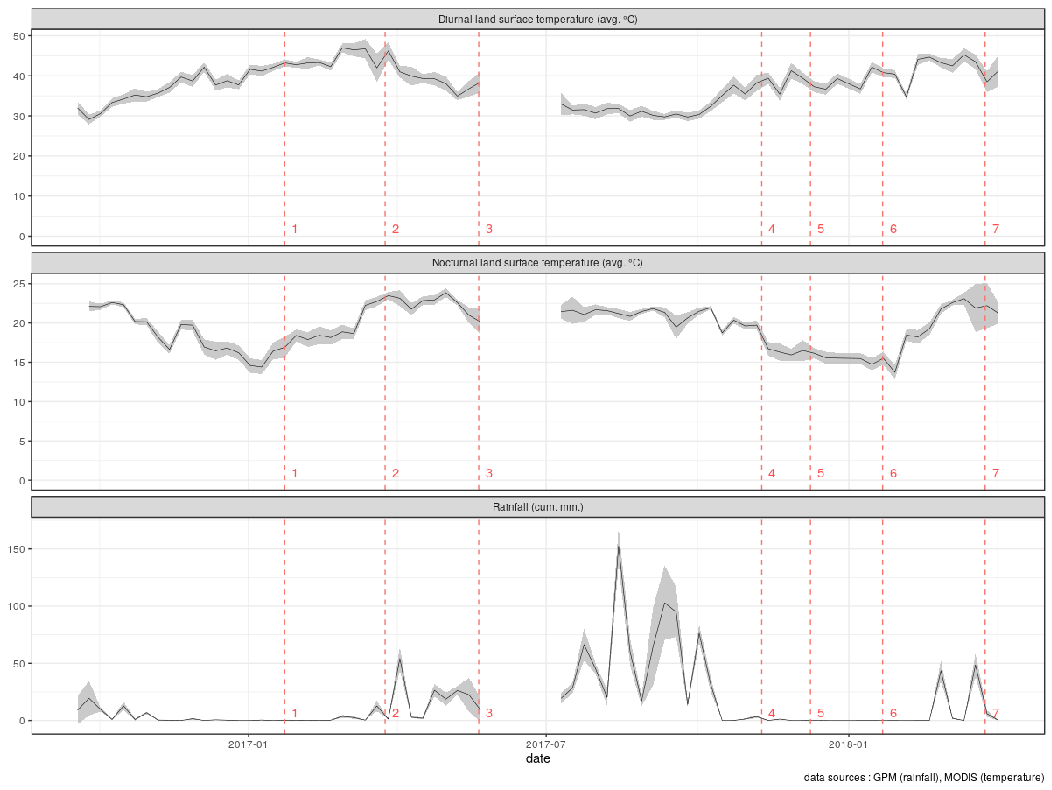
\includegraphics[width=0.8\linewidth]{figure/add_file_1} 

}

\caption[Article n°1 - Figure additionnelle n°1]{Figure additionnelle n°1 : Summary of the meteorological conditions around the sampling points. Average meteorological conditions in a 2 km radius buffer zone around the collection points (weekly aggregation). Vertical red lines indicate the dates of the entomological surveys. Ribbons indicate the mean ± one standard deviation considering all the sampling points.}\label{fig:add-file-1}
\end{figure}
\begin{figure}

{\centering 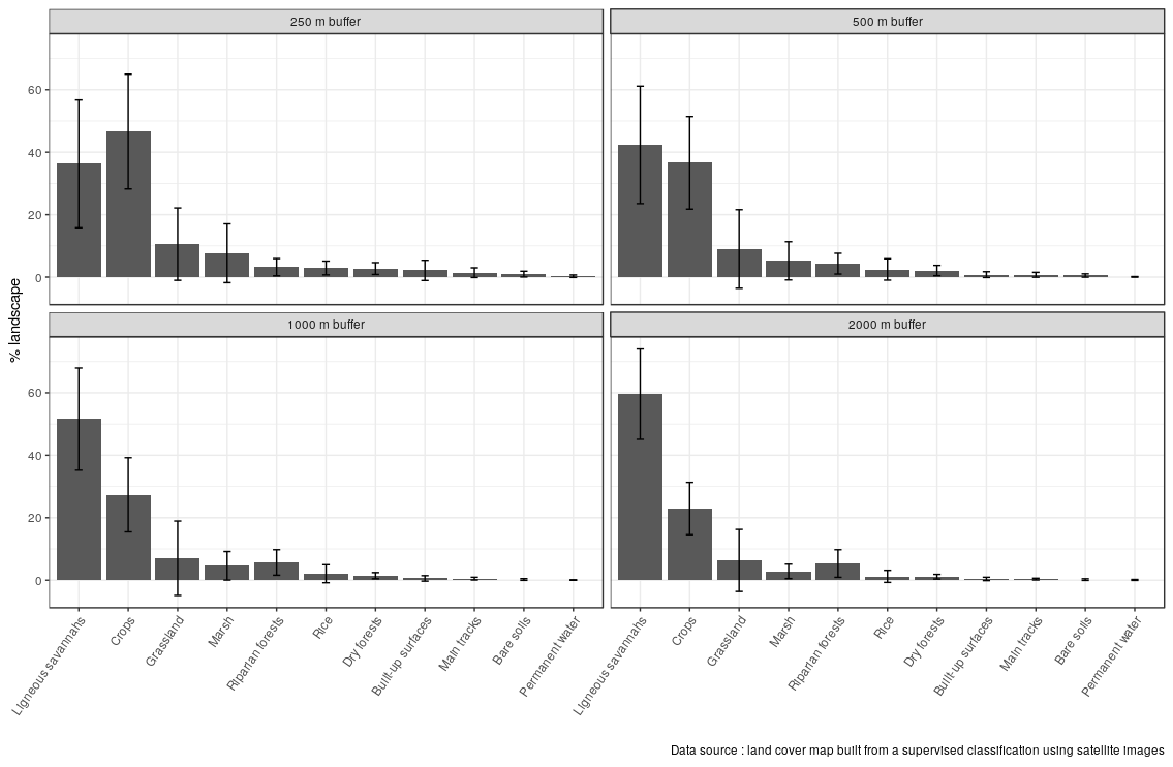
\includegraphics[width=0.8\linewidth]{figure/add_file_2} 

}

\caption[Article n°1 - Figure additionnelle n°2]{Figure additionnelle n°2 : Summary of the landscape conditions around the sampling points. Average percentage of surface occupied by each land cover class in the various buffer zones (250 m, 500 m, 1 km, 2 km radii) around the collection points. Error bars indicate the mean ± one standard deviation considering all the sampling points.}\label{fig:add-file-2}
\end{figure}
\begin{figure}

{\centering 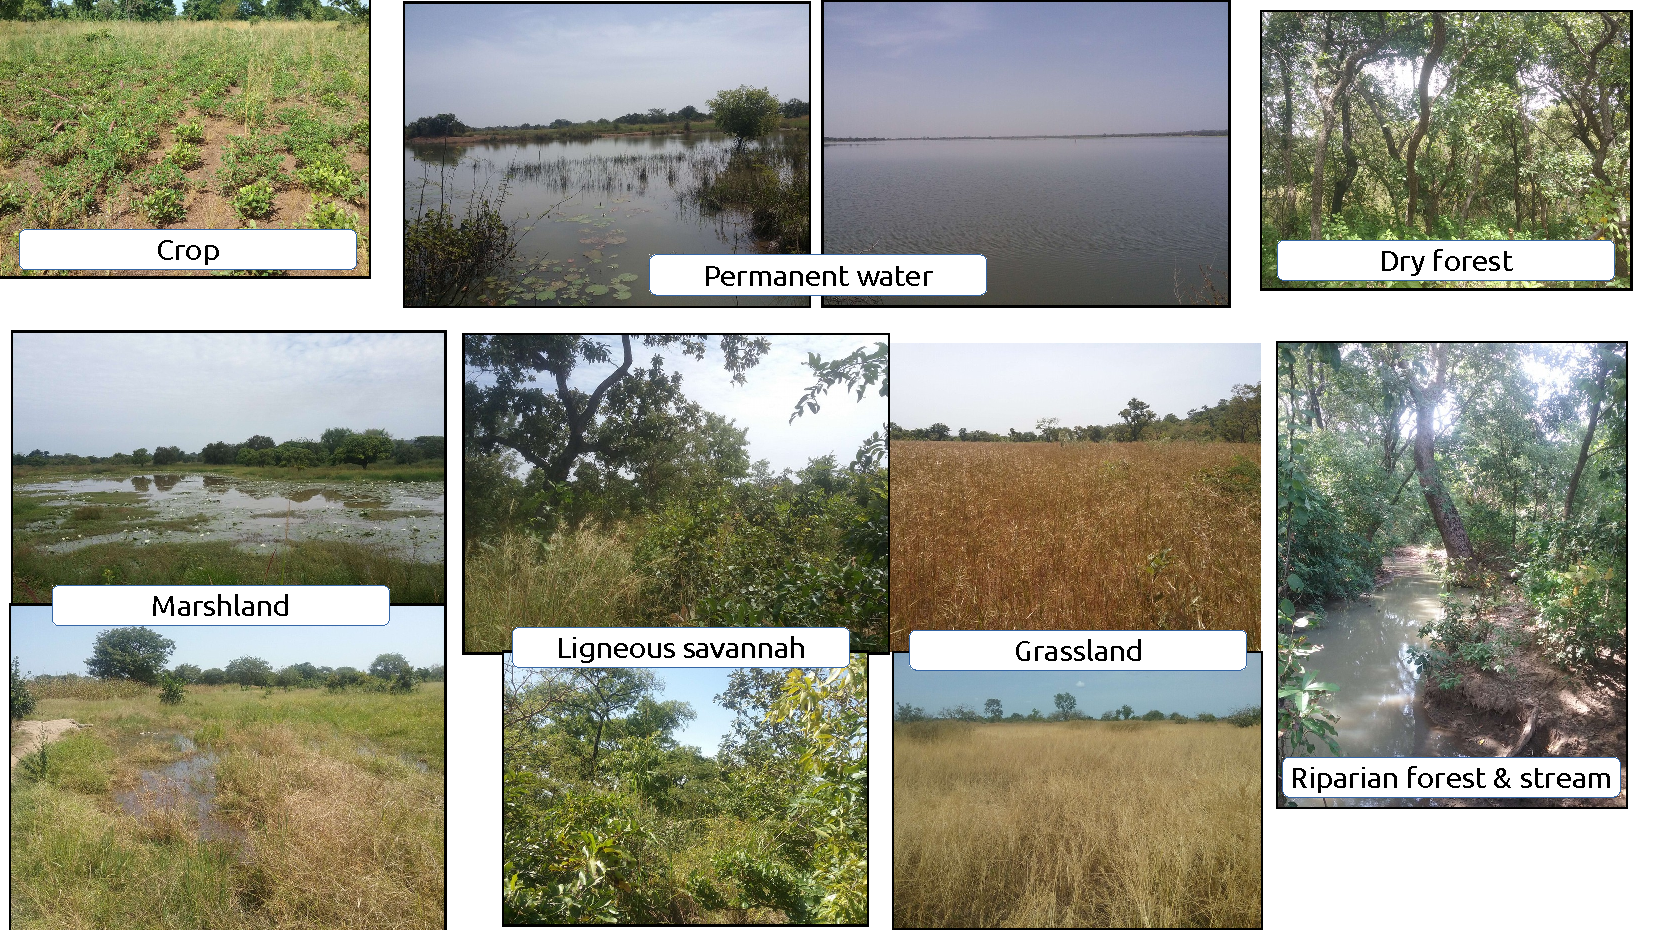
\includegraphics[width=1\linewidth]{figure/add_file_3} 

}

\caption[Article n°1 - Figure additionnelle n°3]{Figure additionnelle n°3 : Pictures representative of the main land cover classes in the Diébougou area. Pictures were taken in November 2018.}\label{fig:add-file-3}
\end{figure}
\begin{figure}

{\centering 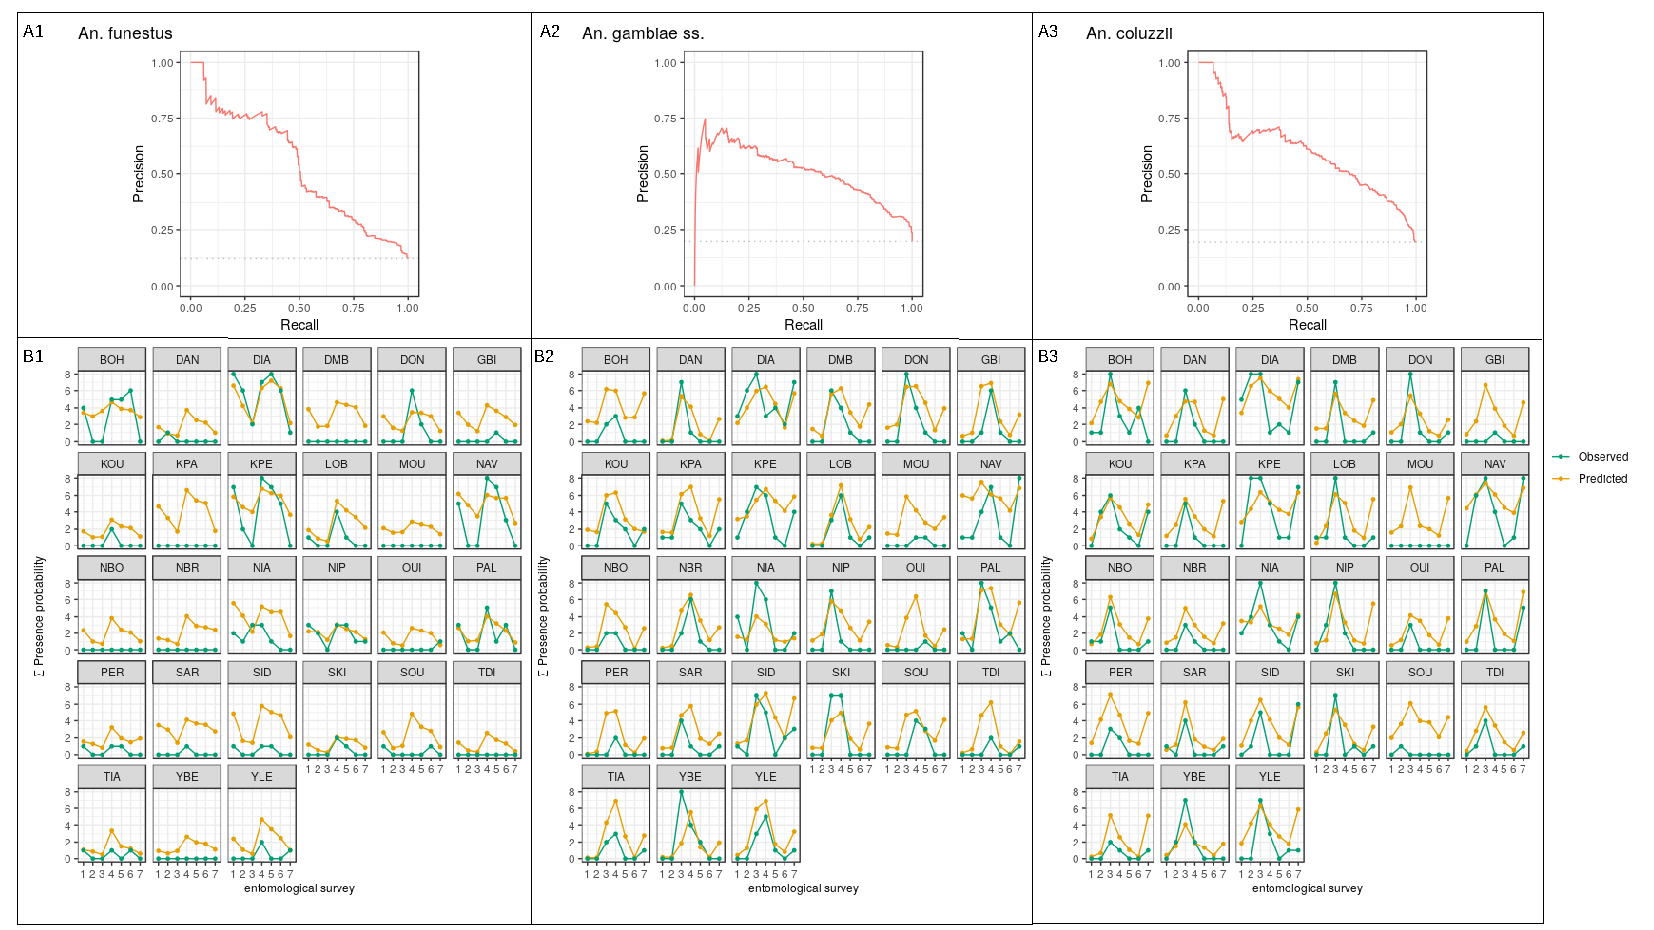
\includegraphics[width=1\linewidth]{figure/add_file_4} 

}

\caption[Article n°1 - Figure additionnelle n°4]{Figure additionnelle n°4 : Model evaluation plots for the presence models. A1, A2, A3 are precision–recall curves for the presence models of respectively An. funestus, An. gambiae s.s. and An. coluzzii. Precision–recall curves show the precision and the recall of the models for different probability thresholds of the “presence” class. Precision is the proportion of presence identifications that was actually correct, while recall is the proportion of actual presence observations that were identified correctly. The horizontal dashed line represents the baseline (i.e. random or no-skill) classifier. A precision–recall curve above the horizontal line indicates a better-than-no-skill classifier. The higher the area between the precision–recall curve and the horizontal line, the better the classifier. Plots B1, B2, B3 are observed vs. predicted presence probabilities for each out-of-sample village. The y-axis represents the sum over the 8 sampling points/village/ survey (4 points by village * 2 places (interior and exterior)). Overall, the plots A1, A2, A3 show that the models had good predictive accuracies (precision–recall curves are higher than the baseline curve, particularly for An. funestus and An. coluzzii). The plots B1, B2, B3 show that the models predicted well the spatiotemporal trends of presence/absence of bites (lines of predicted presence probabilities are generally close to lines of observed probabilities), although they usually slightly overestimated the probabilities of being bitten (predicted presence probability > observed presence probability).}\label{fig:add-file-4}
\end{figure}
\begin{figure}

{\centering 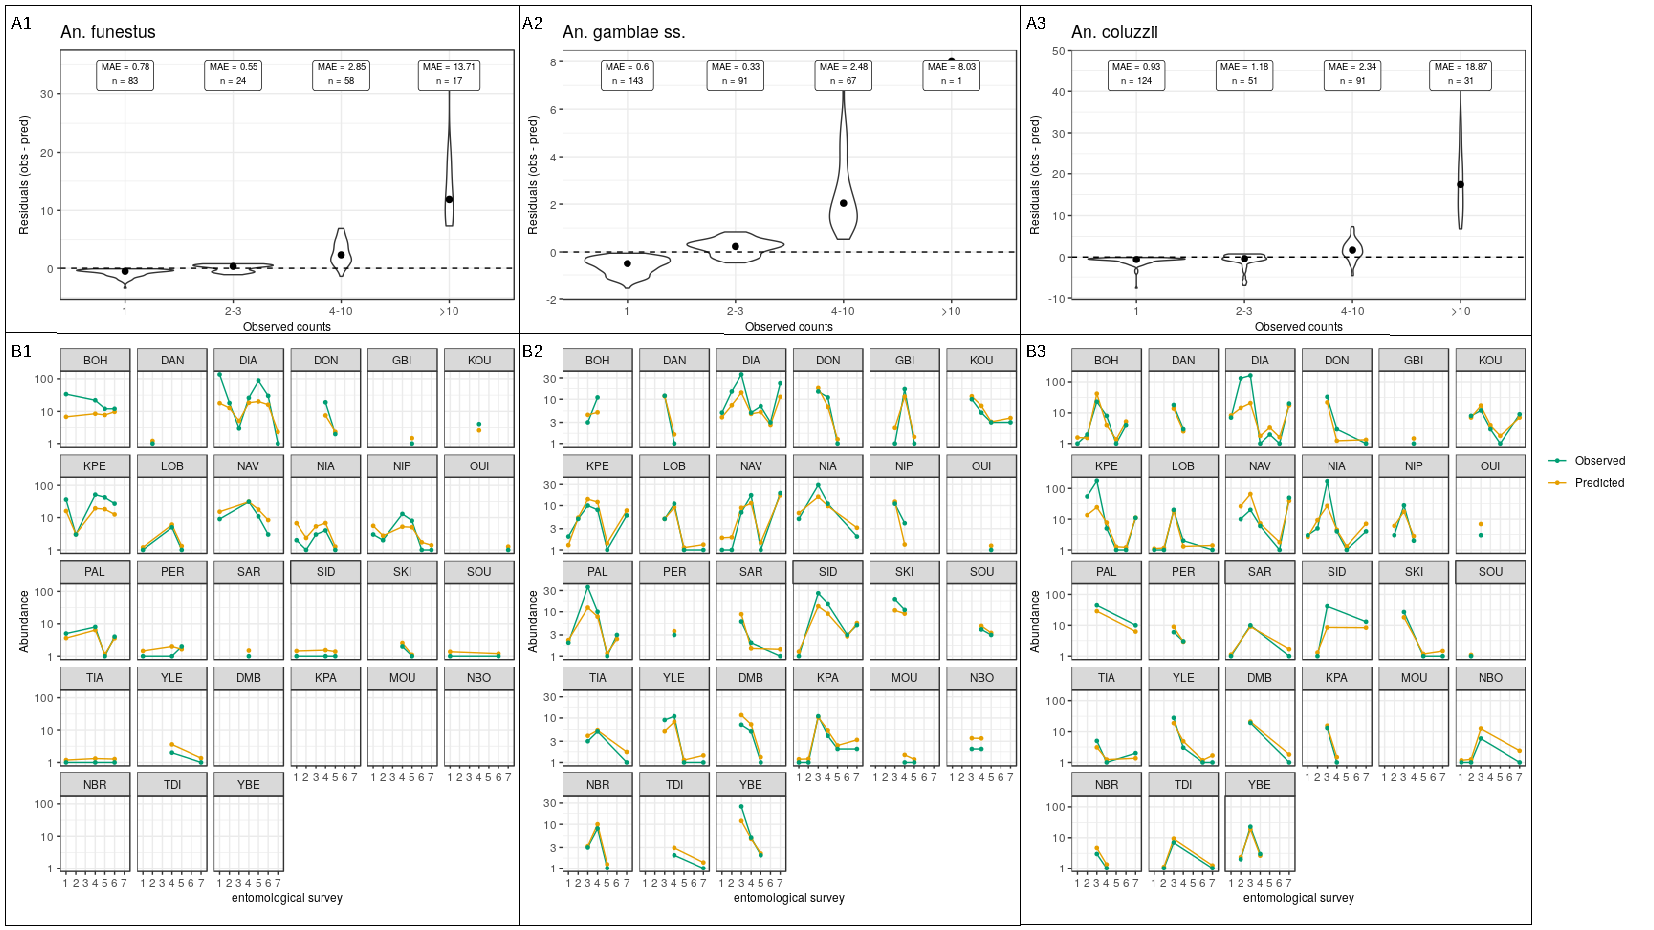
\includegraphics[width=1\linewidth]{figure/add_file_5} 

}

\caption[Article n°1 - Figure additionnelle n°5]{Figure additionnelle n°5 : Model evaluation plots for the abundance models. A1, A2, A3 are violin plots of the distribution of the residuals for the abundance models of respectively An. funestus, An. gambiae s.s. and An. coluzzii, by observed counts of bites (4 classes: 1 bite, 2–3 bites, 4–10 bites, > 10 bites). Black dots indicate the median value. B1, B2, B3 are observed vs. predicted number of bites/village/entomological surveys. The y-axis represents the sum of bites over the 8 sampling points/village/survey (4 points by village * 2 places (interior and exterior)) on a logarithmic scale. The absence of a dot indicates that no vector was collected. MAE = mean absolute error; n = number of observations. Overall, the plots A1, A2, A3 show that the models predicted well small observed counts of bites (1 bite, 2–3 bites) (cf. small MAEs, small residuals), which represent the vast majority of observations (high n). Larger counts (4–10 bites, > 10 bites) tended to be underestimated by the models, especially for An. funestus and An. gambiae s.s. However, large counts (> 10 bites) represented few observations (small n). The plots B1, B2, B3 confirm these observations, and additionally show that general trends of biting rates over time were well predicted by the models (lines of predicted abundance are generally close to lines of observed abundance).}\label{fig:add-file-5}
\end{figure}
\pagebreak

Ci-dessous : Article n°1 - Figure additionnelle n°6 : Feature selection for the multivariate models. The figure shows the Spearman correlation coefficient between the explanatory variables and each response variable (presence and abundance of An. funestus, An. gambiae s.s. and An. coluzzii). Based on these results, variables were retained for the multivariate models according to the following criteria: we first excluded variables that were poorly correlated with the response variable (i.e.~correlation coefficients less than 0.1 or p-values greater than 0.2 at all time associations or buffer radii considered), except for variables related to the presence of water ---i.e.~possible breeding sites---that were all retained whatever their correlation. Then, for each meteorological (resp. landscape) variable, we retained the time lag interval (resp. buffer radius) showing the higher absolute correla- tion coefficient value. We finally excluded collinear variables (i.e.~Pearson correlation coefficient between the variables \textgreater{} 0.7) based on empirical knowledge.\\

\begingroup 
\renewcommand{\headrulewidth}{0pt}

\markboth{}{}

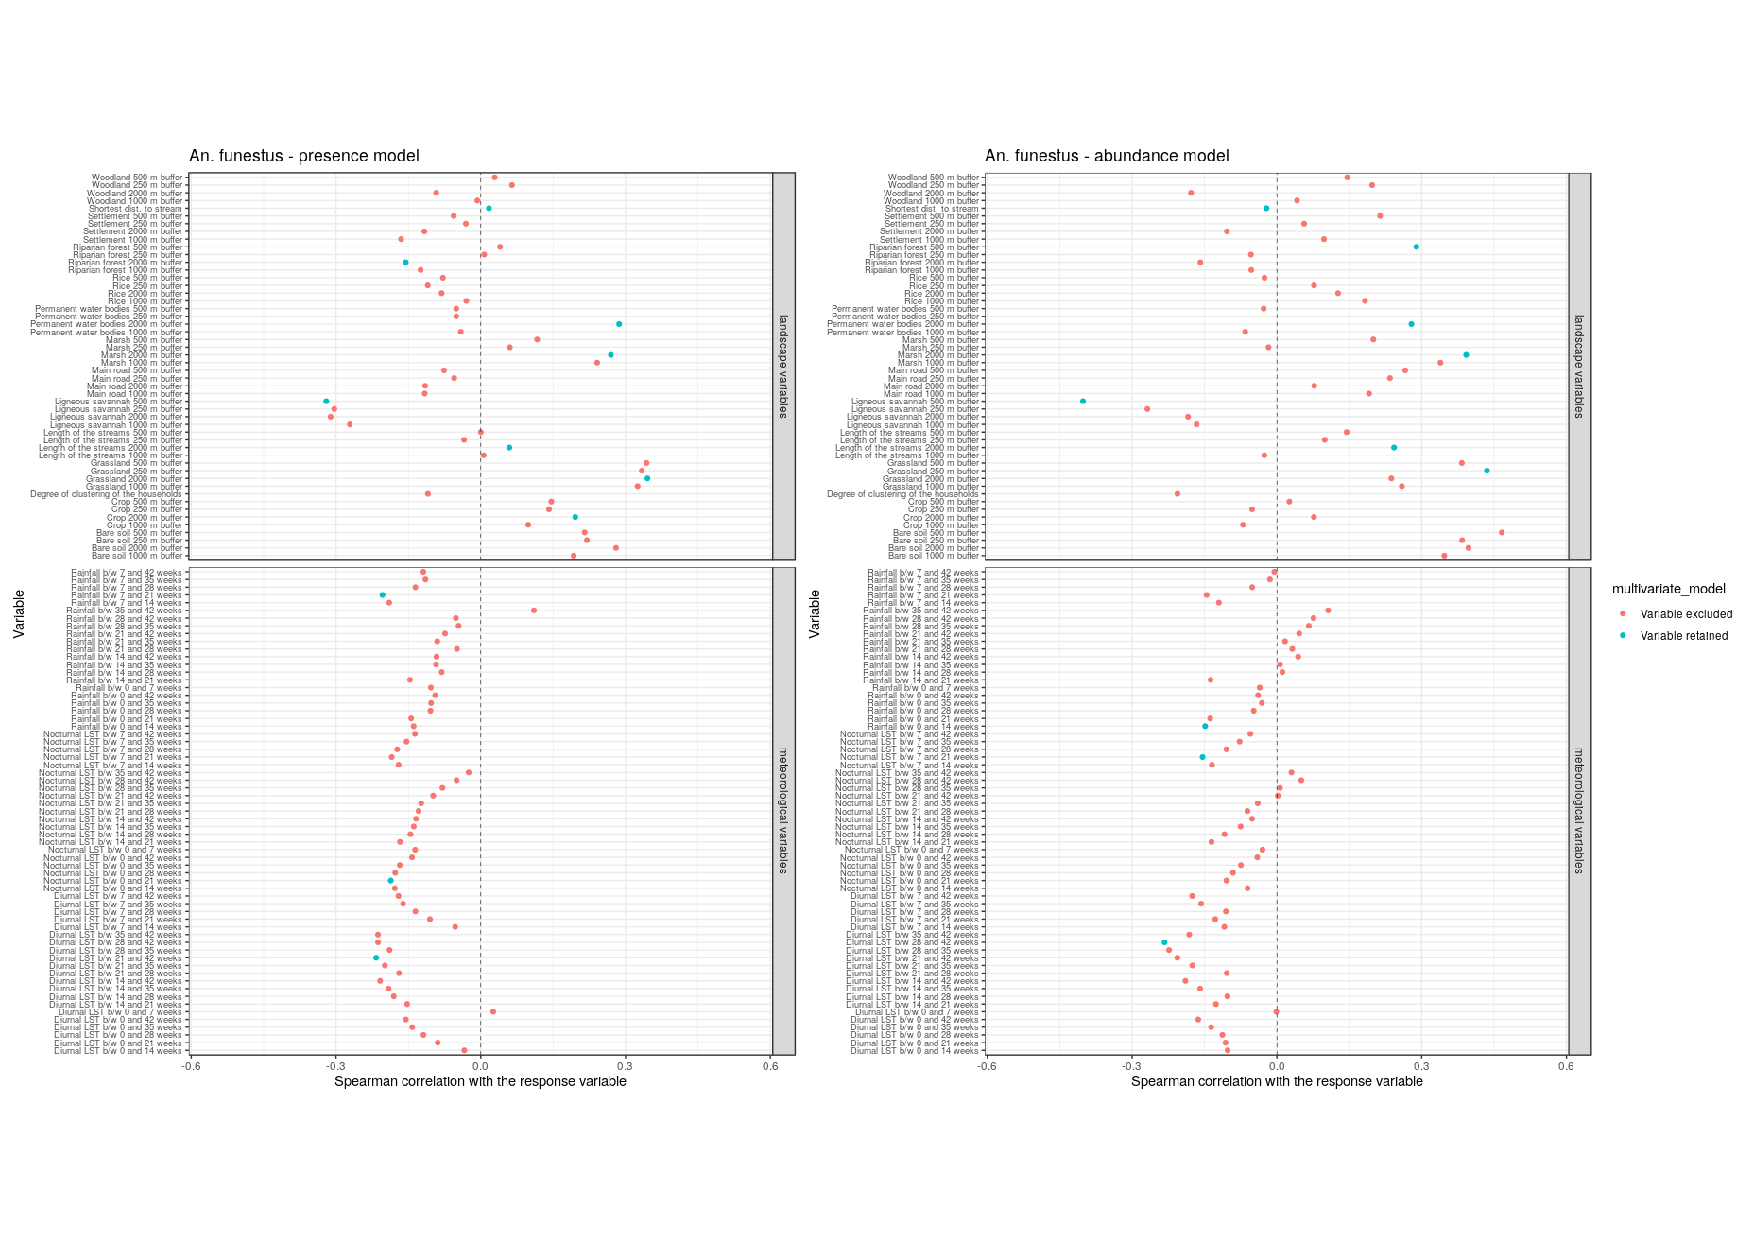
\includepdf[pages=-,nup=1,pagecommand={}]{add_file_6.pdf}
\endgroup

\hypertarget{repro-article-korhogo}{%
\section{Reproduction de l'analyse dans la zone d'étude de Korhogo}\label{repro-article-korhogo}}

Nous avons reproduit l'analyse dans la zone d'étude de Korhogo selon les méthodes décrites dans l'article. Sans entrer dans le niveau de détail de l'article, la section ci-après présente les résultats ainsi qu'une discussion, en détaillant notamment les principales similitudes et différences par rapport aux résultats obtenus dans la zone de Diébougou.

\hypertarget{ruxe9sultats}{%
\subsubsection{Résultats}\label{ruxe9sultats}}

\hypertarget{distribution-spatio-temporelle-des-densituxe9s-agressives-des-anophuxe8les.}{%
\paragraph{Distribution spatio-temporelle des densités agressives des anophèles.}\label{distribution-spatio-temporelle-des-densituxe9s-agressives-des-anophuxe8les.}}

Dans la zone de Korhogo (CI), un total de 2048 nuits-homme de capture a été réalisé (32 villages * 8 enquêtes entomologiques * 4 points de collecte * 2 lieux). 57722 anophèles ont été collectés. Les principales espèces/complexes trouvés étaient \emph{An. gambiae s.l.} et \emph{An. funestus} (respectivement 56267 (97\% de tous les anophèles collectés) et 714 (1\%) individus collectés). Parmi les 56267 \emph{An. gambiae s.l.} collectés, 3922 (7\%) ont été identifiés à l'espèce : 3726 (95\% des individus identifiés à l'espèce) étaient des \emph{An. gambiae s.s.} et 196 (5\%) étaient des \emph{An. coluzzii}. Par conséquent, dans la suite de cette étude, nous considérerons les \emph{An. gambiae s.l.} collectés dans la zone de Korhogo comme des \emph{An. gambiae s.s.}\\

\emph{An. gambiae s.s.} et \emph{An. funestus} étaient présents (cad. au moins un anophèle capturé) dans respectivement 64 \% et 6 \% des nuits-homme de capture. La distribution des densités agressives sur les sessions positives (cad. au moins un contact homme-vecteur) était très asymétrique, comme dans la zone de Diébougou (pour \emph{An. gambiae s.s.} : médiane = 18, écart-type = 65, max. = 505 ; pour \emph{An. funestus} : médiane = 2, écart-type = 12, max. = 84). La figure \ref{fig:map-bitingrates-ci} présente les distributions spatio-temporelles des densités agressives des principales espèces d'anophèles dans la zone de Korhogo (pendant de la fig.~1 de l'article). La carte montre des dynamiques temporelles pour \emph{An. gambiae s.s.} relativement similaires à celles de la zone de Diébougou : l'espèce était davantage abondante durant ou en fin de saison pluvieuse (septembre, octobre) qu'en saison sèche, où elle était malgré tout présente. Au niveau spatial, notons i) une certaine hétérogénéité de la distribution, et ii) que l'espèce était présente dans quasiment tous les villages à toutes les enquêtes entomologiques (sauf la 7ème), contrastant avec la zone de Diébougou où l'espèce était absente de plusieurs villages. La distribution spatio-temporelle d'\emph{An. funestus} était très déséquilibrée : l'écrasante majorité des individus (93 \%) a été collectée lors de la première enquête entomologique, et presque la moitié des individus (42 \%) a été collecté dans un seul village.\\
\begin{figure}

{\centering 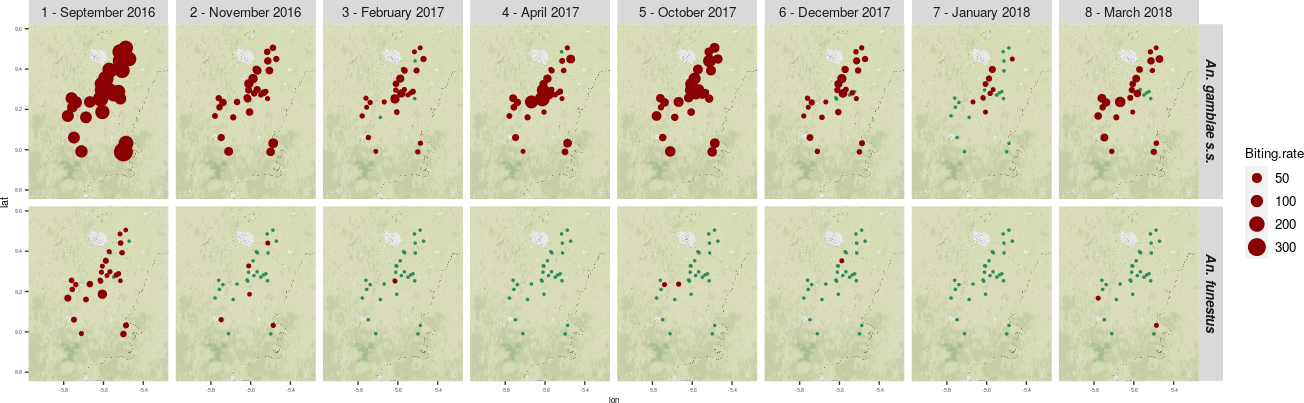
\includegraphics[width=1.1\linewidth]{figure/map_bitingrates_ci} 

}

\caption[Distribution spatio-temporelle des densités agressives des principales espèces d'anophèles dans la zone de Korhogo]{Distribution spatio-temporelle des densités agressives des principales espèces d'anophèles dans la zone de Korhogo (voir légende complète dans la figure 1 de l'article en section \ref{full-article-1} )}\label{fig:map-bitingrates-ci}
\end{figure}
\hypertarget{moduxe9lisation-bivariuxe9e.}{%
\paragraph{Modélisation bivariée.}\label{moduxe9lisation-bivariuxe9e.}}

La figure \ref{fig:spbuffer-ci} montre les variables paysagères qui étaient significativement corrélées (coefficient de corrélation de Spearman (cc) \textgreater{} 0.1 et p.value \textless{} 0.2) avec la présence et l'abondance des espèces d'anophèles (pendant de la fig.~3 de l'article). Comme à Diébougou, la présence et l'abondance d'\emph{An. funestus} était corrélée à davantage de variables paysagères que celle d'\emph{An. gambiae s.s.}, et les coefficients de corrélation les plus élevés avec les variables paysagères étaient observés pour \emph{An. funestus}.
\begin{figure}

{\centering 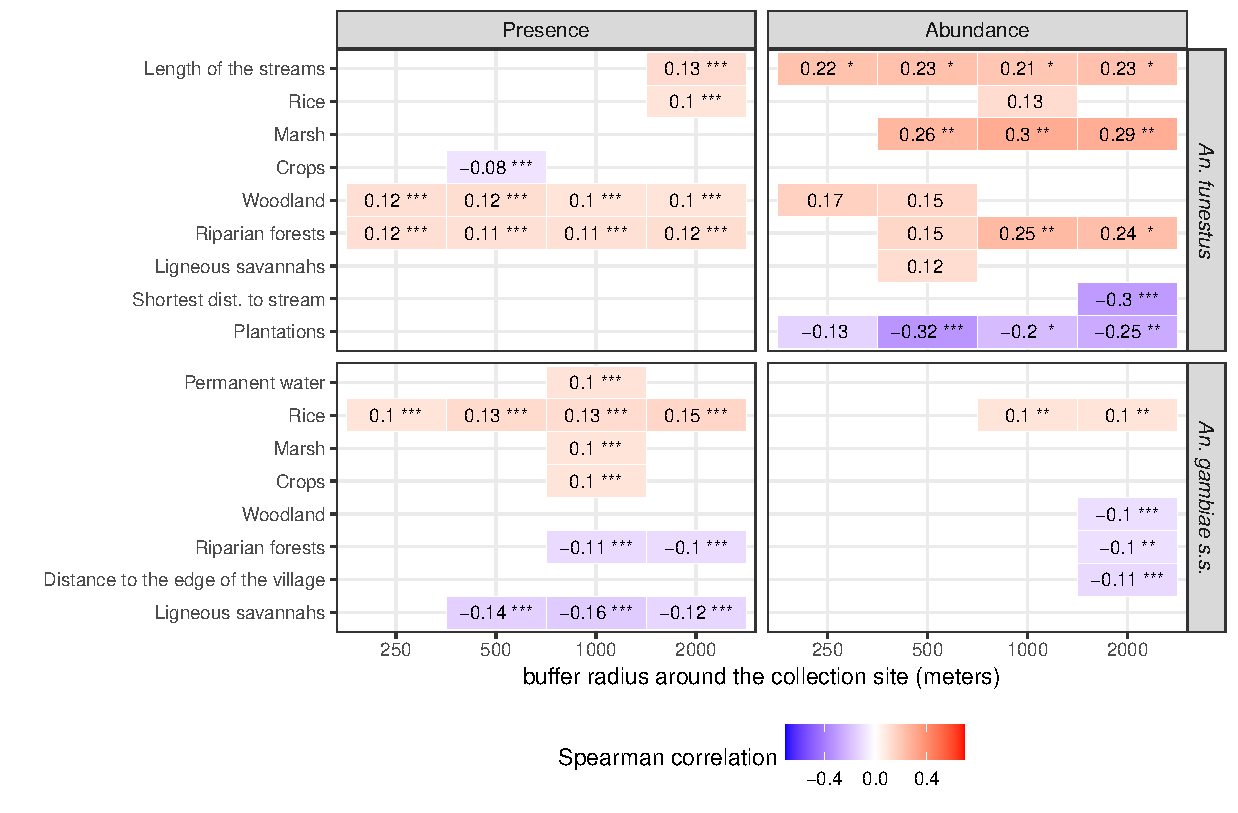
\includegraphics[width=1\linewidth]{figure/spatialbuffer_ci} 

}

\caption[Coefficient de corrélation de Spearman entre entre les densités agressives des anophèles et les variables paysagères dans la zone de Korhogo]{Coefficient de corrélation de Spearman entre entre les densités agressives des anophèles et les variables paysagères dans la zone de Korhogo (voir légende complète dans la figure 3 de l'article en section \ref{full-article-1})}\label{fig:spbuffer-ci}
\end{figure}
La présence d'\emph{An. funestus} était positivement corrélée avec la longueur des rivières et au \% de surface occupé par les zones rizicoles, dans la zone tampon de 2 km de rayon. Elle était également corrélée avec le \% de surface occupé par les forêts ripicoles et les zones forestières (non ripicoles), dans toutes les zones tampon. L'abondance de l'espèce était positivement corrélée avec la longueur des rivières, les surfaces rizicoles, les surfaces marécageuses, les forêts ripicoles, et les zones forestières (non ripicoles), dans diverses tailles de zone tampon en fonction de la classe d'occupation du sol. L'abondance d'\emph{An. funestus} était négativement corrélée avec le \% de surface occupé par les plantations dans la zone tampon de 2 km de rayon, et avec à la distance à la rivière la plus proche (autrement dit, l'abondance était plus importante quand le point de capture était proche d'une rivière).\\

La présence d'\emph{An. gambiae s.s.} était positivement corrélée avec le \% de surface en eaux permanentes, en zones marécageuses, et en zones agricoles dans la zone tampon d'1 km de rayon. La présence ainsi que l'abondance de l'espèce étaient également corrélée avec le \% de surface occupée par les zones rizicoles, dans toutes les zones tampon pour la présence et dans les zones tampons d'1 et 2 km de rayon pour l'abondance. La présence et l'abondance d'\emph{An. gambiae s.s.} était négativement corrélées avec le \% de surface occupé par les forêts ripicoles, dans les zones tampons d'1 et 2 km de rayon pour la présence et dans la zone de 2 km pour l'abondance. L'abondance de l'espèce était négativement corrélée avec le \% de surface occupée par les zones forestières dans la zone tampon de 2 km de rayon, et avec la distance à la lisière du village (autrement dit, l'abondance était plus importante dans les habitations situées proches de la lisière du village que dans celles situées proches du centre du village). La présence de l'espèce était négativement corrélée avec le \% de surface occupée par les savanes ligneuses, dans les zones tampons de plus de 250 m de rayon.\\

Notons que les valeurs absolues des coefficients de corrélation entre la présence / abondance des espèces et les variables paysagères étaient, dans l'ensemble, moins élevées dans la zone de Korhogo que dans la zone de Diébougou.\\

La figure \ref{fig:ccm-ci} montre les variables météorologiques qui étaient significativement corrélées (coefficient de corrélation de Spearman (cc) \textgreater{} 0.1 et p.value \textless{} 0.2) avec la présence et l'abondance des espèces d'anophèles (\emph{cross-correlation maps}, ou CCM) (pendant de la fig.~4 de l'article). Comme à Diébougou, les coefficients de corrélation entre la présence/abondance des espèces et les variables météorologiques étaient plus élevés pour \emph{An. gambiae s.s.} que pour \emph{An. funestus}.
\begin{figure}

{\centering 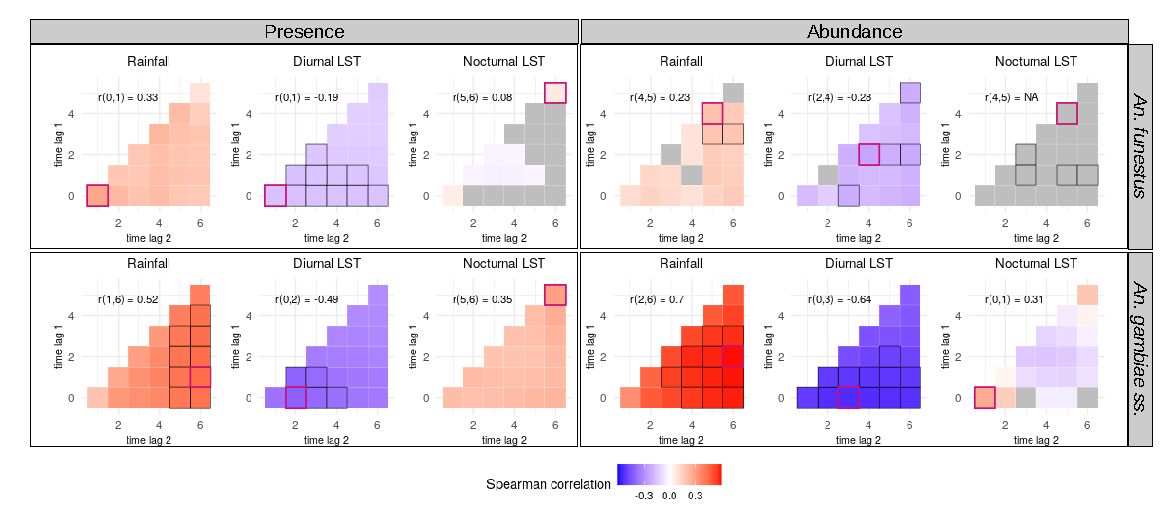
\includegraphics[width=1.1\linewidth]{figure/ccm_ci} 

}

\caption[Coefficient de correlation de Spearman entre entre les densités agressives des anophèles et les variables météorologiques dans la zone de Korhogo (sous forme de cross-correlation maps)]{Coefficient de correlation de Spearman entre entre les densités agressives des anophèles et les variables météorologiques dans la zone de Korhogo (sous forme de cross-correlation maps) (voir légende complète dans la figure 4 de l'article en section \ref{full-article-1})}\label{fig:ccm-ci}
\end{figure}
La présence et l'abondance d'\emph{An. funestus} étaient positivement corrélées avec le cumul des précipitations précédant la date de capture, à presque tous les `lags' temporels - ce qui contraste avec la zone de Diébougou où les corrélations d'\emph{An. funestus} avec les précipitations étaient négatives. La présence et l'abondance de l'espèce étaient négativement corrélées avec les températures diurnes, là aussi à presque tous les lags temporels précédant la date de capture. Les corrélations entre la présence ou l'abondance d'\emph{An. funestus} et les températures nocturnes précédant la date de capture étaient faibles ou non-significatives.\\

La présence et l'abondance d'\emph{An. gambiae s.s.} était positivement, fortement corrélées (plus encore qu'à Diébougou) avec le cumul des précipitations précédant la date de capture, à tous les lags temporels. Parmi tous les lags, c'est le cumul des précipitations enregistré entre les semaines 1 à 6 précédant la capture qui présentait le coefficient de corrélation le plus élevé avec la présence de l'espèce ; et le cumul des précipitations enregistré entre les semaines 2 à 6 précédant la capture qui présentait le coefficient de corrélation le plus élevé avec l'abondance de l'espèce. La présence d'\emph{An. gambiae s.s.} était également positivement corrélée avec les températures nocturnes précédant la date de capture à tous les lags temporels, et le coefficient de corrélation maximum était entre 5 et 6 semaines avant la capture. La présence et l'abondance d'\emph{An. gambiae s.s.} était négativement corrélée avec les températures diurnes précédant la date de capture, à tous les lags temporels. Le coefficient de corrélation maximum entre les températures diurnes et la présence/abondance de l'espèce était entre 0 et 2-3 semaines avant la date de capture. Notons que les CCM (\emph{Cross-Correlation Maps}) d'\emph{An. gambiae s.s.} dans les zones de Korhogo et Diébougou étaient, une à une, très semblables : si les valeurs absolues des coefficients de corrélation étaient globalement légèrement supérieures dans la zone de Korhogo, les lags temporels présentant les coefficients de corrélation les plus élevés étaient quasiment identiques pour 5 des 6 CCMs.\\

Notons qu'à l'inverse des variables paysagères, les valeurs absolues des coefficients de corrélation entre la présence / abondance des espèces et les variables météorologiques étaient, dans l'ensemble, plus élevés dans la zone de Korhogo que dans la zone de Diébougou (en particulier pour \emph{An. gambiae s.s.}).

\hypertarget{moduxe9lisation-multivariuxe9e.}{%
\paragraph{Modélisation multivariée.}\label{moduxe9lisation-multivariuxe9e.}}

La \emph{Precision-Recall area under the curve} (PR-AUC) des modèles de présence était de 0.52 (baseline=0.09) et 0.91 (baseline=0.64) pour \emph{An. funestus} et \emph{An. gambiae s.s.} respectivement. La spécificité et la sensitivité des modèles au seuils optimaux de probabilité de présence étaient de 53 \% et 98 \% pour \emph{An. funestus} et de 88 \% et 61 \% pour \emph{An. gambiae s.s.} Ces résultats indiquent de bonnes puissance prédictives pour les modèles de présence, comme dans la zone de Diébougou. De même, comme dans la zone BF, les modèles d'abondance refletaient bien les tendances des abondances observées. Les figures d'évaluation des modèles multivariés de présence et d'abondance dans la zone de Korhogo (pendant des `supplementary file' 4 et 5 de l'article) sont présentées dans les figures \ref{fig:evaluation-plot-ci-presence} et \ref{fig:evaluation-plot-ci-abundance}.\\
\begin{figure}

{\centering 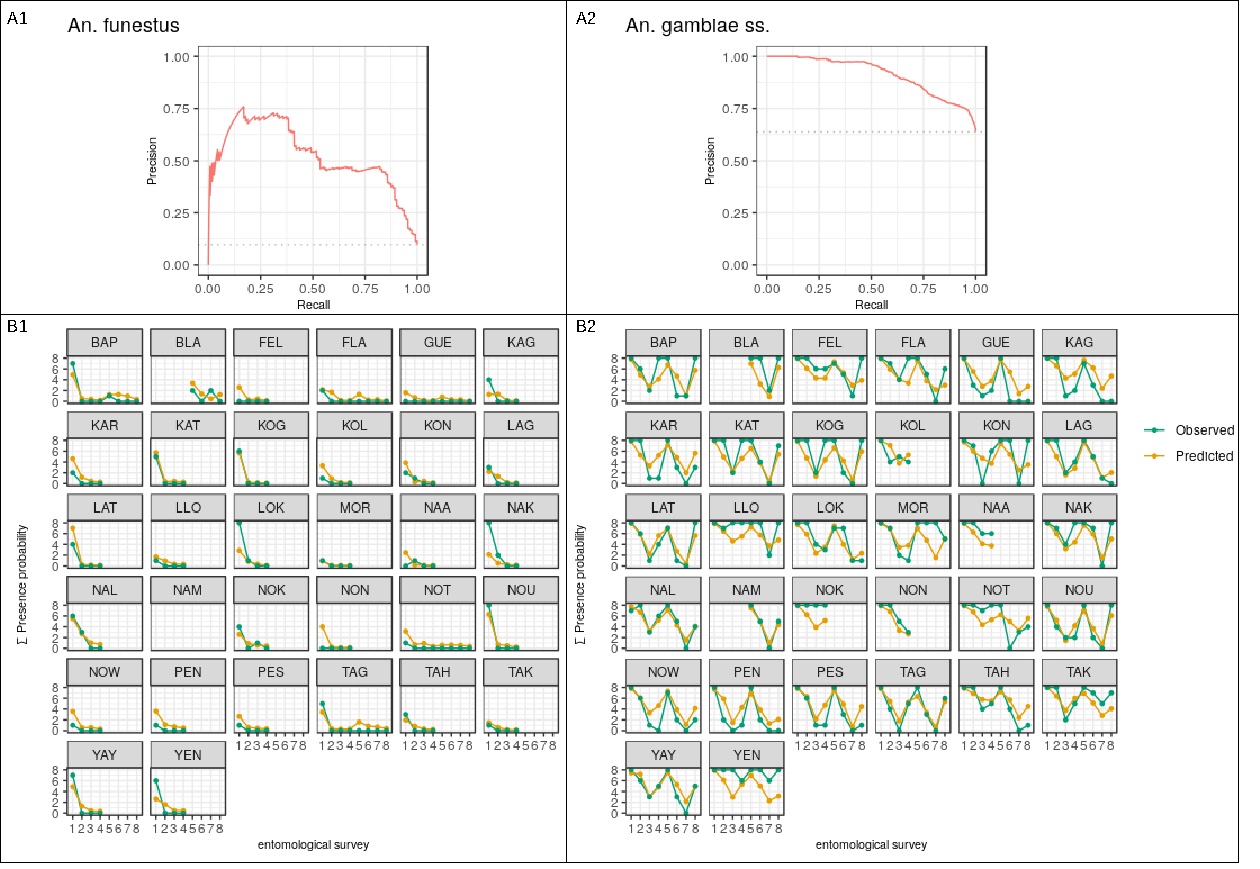
\includegraphics[width=1.1\linewidth]{figure/modelevaluation_ci_presence} 

}

\caption[Evaluation de la puissance prédictive des modèles de présence des anophèles dans la zone de Korhogo]{Evaluation de la puissance prédictive des modèles de présence des anophèles dans la zone de Korhogo (voir légende complète dans la figure additionnelle 5 (Figure S5) de l'article en section \ref{full-article-1})}\label{fig:evaluation-plot-ci-presence}
\end{figure}
\begin{figure}

{\centering 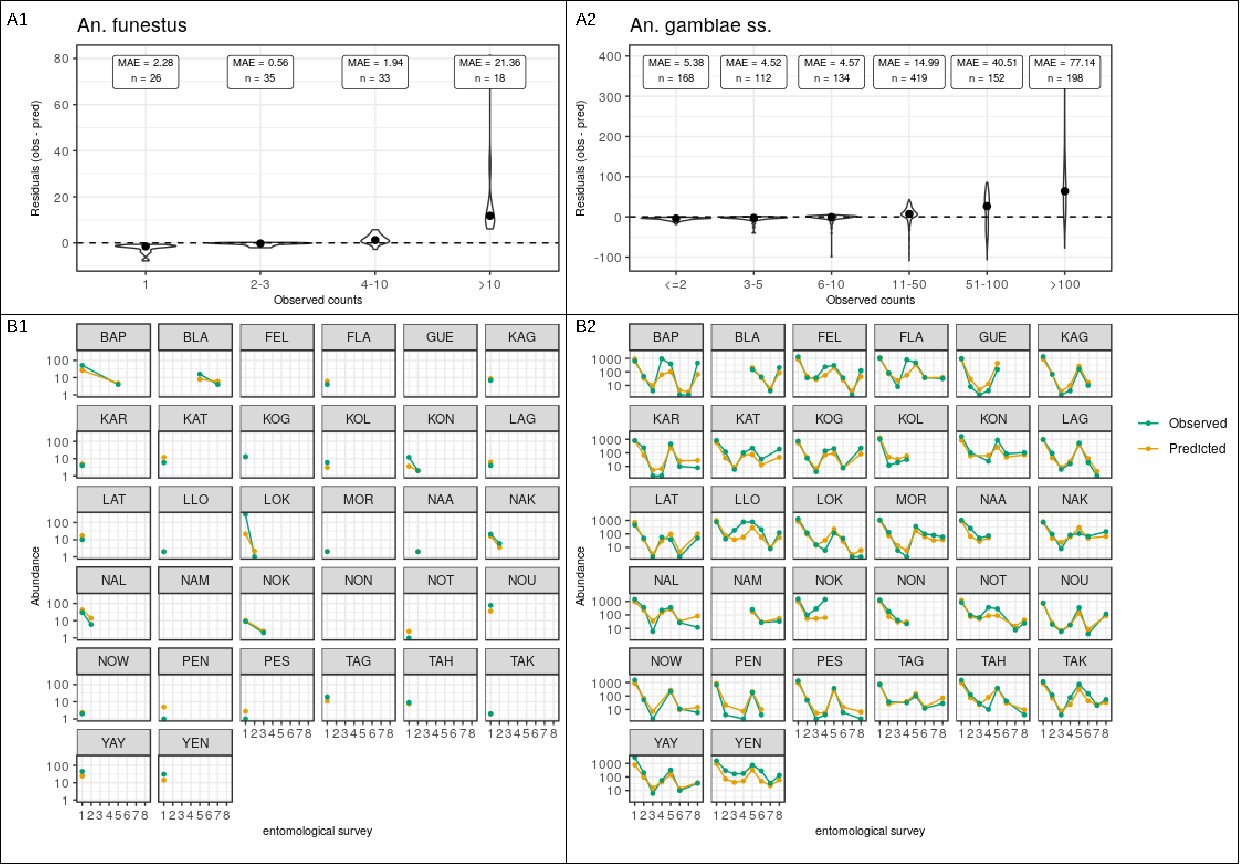
\includegraphics[width=1\linewidth]{figure/modelevaluation_ci_abundance} 

}

\caption[Evaluation de la puissance prédictive des modèles d'abondance des anophèles dans la zone de Korhogo]{Evaluation de la puissance prédictive des modèles de d'abondance des anophèles dans la zone de Korhogo (voir légende complète dans la figure additionnelle 5 (Figure S5) de l'article en section \ref{full-article-1})}\label{fig:evaluation-plot-ci-abundance}
\end{figure}
Les figures \ref{fig:pdp-ci-gambiae} et \ref{fig:pdp-ci-funestus} montrent les graphiques d'interprétation des modèles de forêt aléatoire (variables d'importances et les plots de dépendance partiels) pour la présence et l'abondance des deux espèces (pendant des fig.~5-6-7 de l'article).\\
\begin{figure}

{\centering 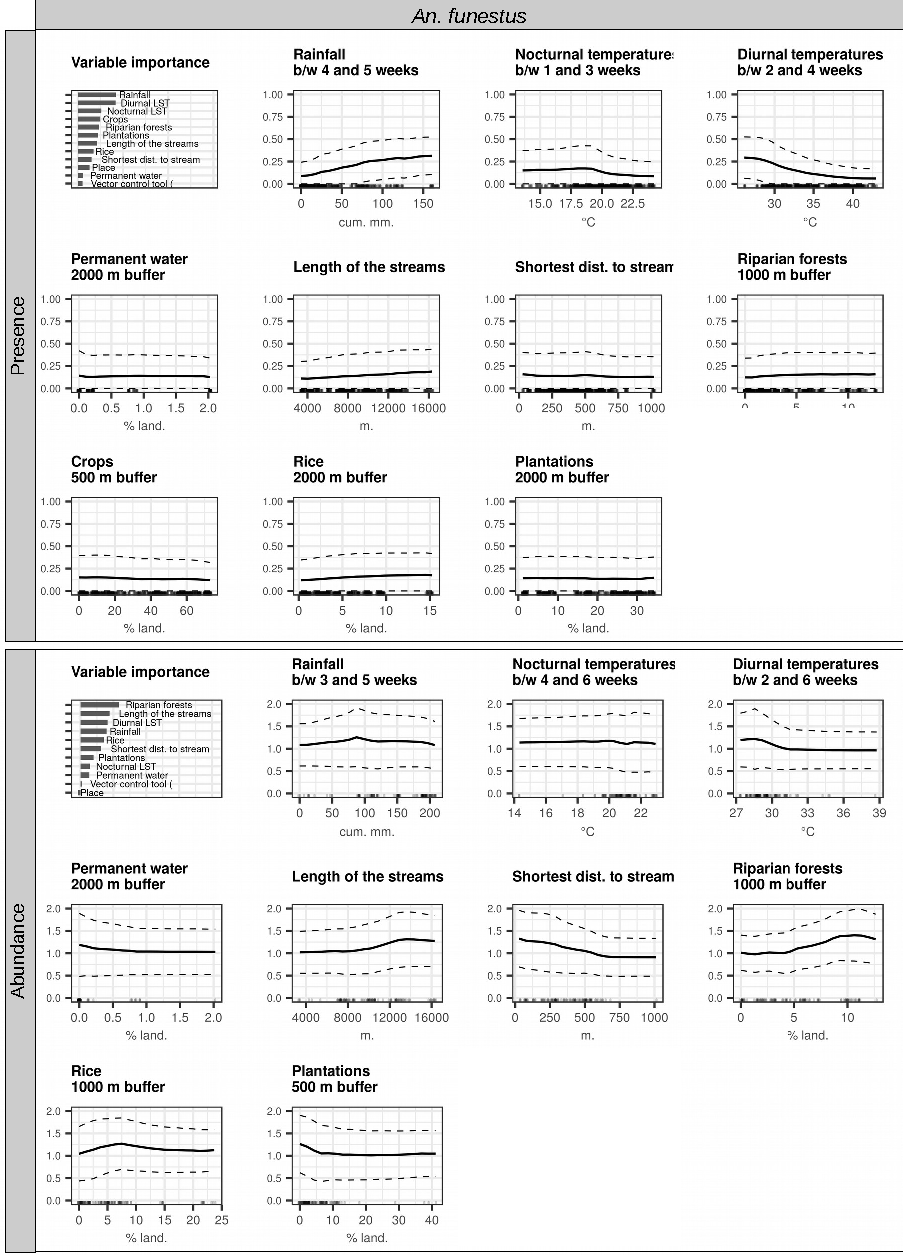
\includegraphics[width=1\linewidth]{figure/pdp_funestus_ci} 

}

\caption[Graphiques d'interprétation des modèles de forêt aléatoires pour An. funestus dans la zone de Korhogo]{Graphiques d'interprétation des modèles de forêt aléatoires pour An. funestus dans la zone de Korhogo (voir légende complète dans la figure 5 de l'article en section \ref{full-article-1})}\label{fig:pdp-ci-funestus}
\end{figure}
Les variables les plus importantes dans le modèle de présence d'\emph{An. funestus} étaient les trois variables descriptives de la météorologie enregistrée pendant les semaines précédant la capture : cumul des précipitations (relation linéaire positive), températures diurnes moyennes (relation négative entre 25°C et 35°C, et plafonnant entre 35° et 45°), et températures nocturnes moyennes. Les variables les plus importantes dans le modèle d'abondance de cette espèce étaient : le \% de surface occupé par les forêts ripicoles (relation nulle entre 0\% et 5\%, positive entre 5\% et 10\%, et nulle entre 10\% et 12\%), la longueur totale des rivières dans la zone tampon de 2 km de rayon autour des points de capture (relation nulle entre 4 km et 10 km de rivières, positive entre 10 km et 13 km, et nulle entre 13 km et 16 km), et les températures diurnes moyennes (relation linéaire négative entre 27°C et 31°C et nulle entre 31°C et 39°C).\\

Les prédicteurs secondaires dans le modèle de présence d'\emph{An. funestus} étaient des variables paysagères : \% de surface occupé par les forêts ripicoles (relation positive linéaire), \% de surface occupé par les rizicultures (relation positive linéaire), la longueur totale des rivières dans la zone tampon de 2 km de rayon autour des points de capture (relation positive linéaire). Les prédicteurs secondaires dans le modèle d'abondance étaient : le \% de surface occupé par les rizicultures (relation positive), la distance à la rivière la plus proche (relation négative), et le \% de surface occupé par les forêts ripicoles (relation positive).\\
\begin{figure}

{\centering 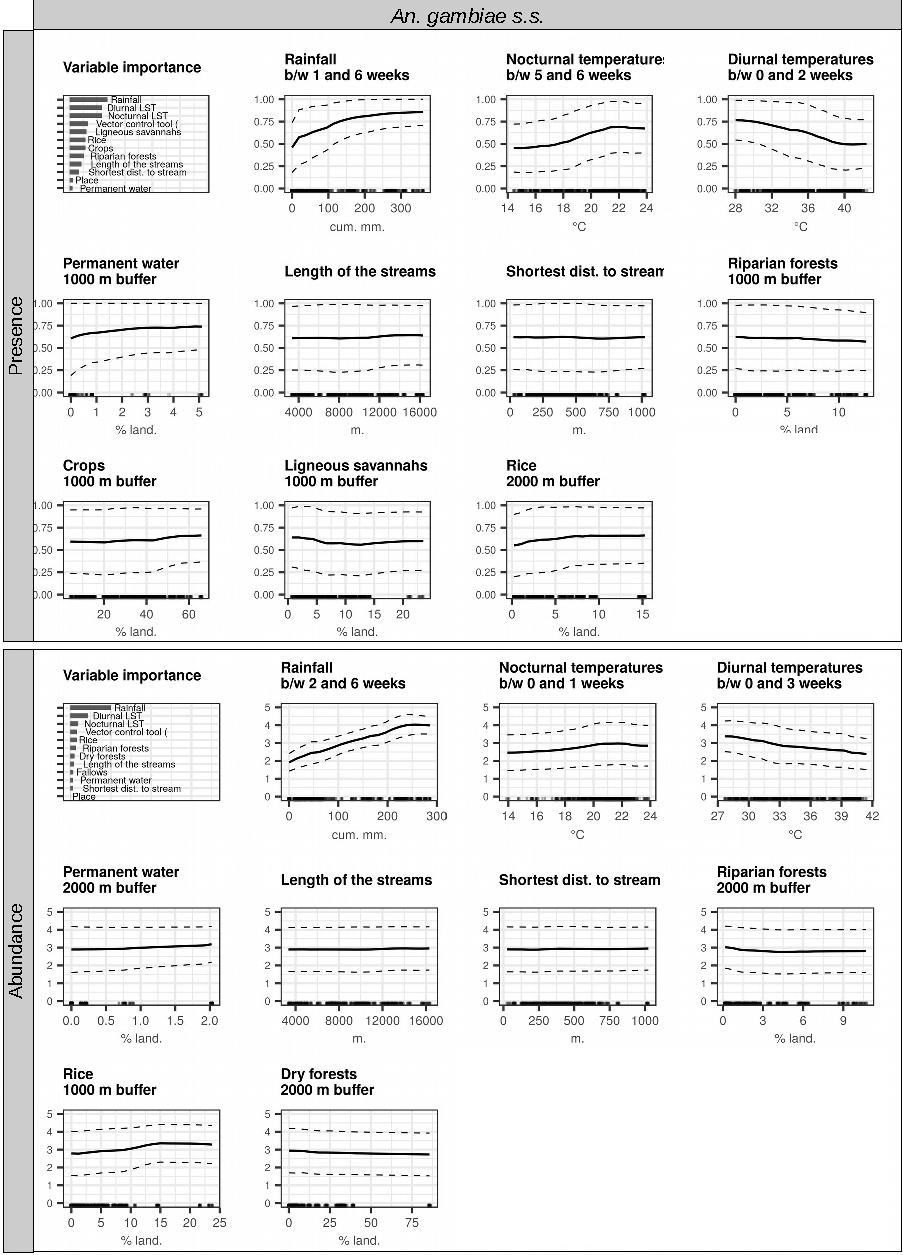
\includegraphics[width=1\linewidth]{figure/pdp_gambiaess_ci} 

}

\caption[Graphiques d'interprétation des modèles de forêt aléatoires pour An. gambiae s.s. dans la zone de Korhogo]{Graphiques d'interprétation des modèles de forêt aléatoires pour An. gambiae s.s. dans la zone de Korhogo (voir légende complète dans la figure 5 de l'article en section \ref{full-article-1})}\label{fig:pdp-ci-gambiae}
\end{figure}
Les variables les plus importantes dans les modèles de présence et d'abondance d'\emph{An. gambiae s.s.} étaient les trois variables descriptives de la météorologie enregistrée pendant les semaines précédant la capture : dans l'ordre, cumul des précipitations entre 1-2 et 6 semaines précédant la capture, températures diurnes moyennes entre 0 et 2-3 semaines précédant la capture, et températures nocturnes moyennes (entre 5 et 6 semaines et entre 0 et 1 semaine pour les modèles de présence et d'abondance respectivement). La probabilité de présence augmentait logarithmiquement avec les précipitations, et l'abondance augmentait linéairement avec les précipitations. La nature des relations avec les températures était relativement similaire à celle d'\emph{An. gambiae s.s.} dans la zone de Diébougou. Notons que l'importance des précipitations était particulièrement élevée dans le modèle d'abondance d'\emph{An. gambiae s.s.}, dominant largement l'importance de toutes les autres variables.\\

Les prédicteurs secondaires dans le modèle de présence d'\emph{An. gambiae s.s.} étaient le \% de surface occupé par les savanes ligneuses (relation négative entre 0\% et 5\% puis nulle entre 5\% et 25\%), le \% de surface occupé par les rizicultures (relation positive entre 0\% et 10\% puis nulle entre 10\% et 15\%), et le \% de surface occupé par les zones agricoles (relation nulle entre 0\% et 50\% puis positive entre 50\% et 60\%). Les prédicteurs secondaires dans le modèle d'abondance étaient le \% de surface occupée par les rizières (relation positive entre 0\% et 15\% puis nulle entre 15\% et 25\%), le \% de surface occupé par les forêts ripicoles (relation négative entre 0\% et 3\% puis nulle entre 3\% et 10\%), et le \% de surface occupé par les forêts (relation négative linéaire).\\

\hypertarget{discussion}{%
\subsubsection{Discussion}\label{discussion}}

Dans la zone de Korhogo, le cumul des précipitations était la variable la plus importante à la fois dans les modèles de présence et d'abondance d'\emph{An. gambiae s.s} ; et dans les deux modèles les variables de températures complétaient le trio de tête des varibles d'importance. Ces observations, similaires à celles effectuées dans la zone de Diébougou, montrent que dans la zone de Korhogo comme sur celle de Diébougou i) \emph{An. gambiae s.s.} était attaché aux gites larvaires temporaires, remplis par les précipitations et ii) ses traits de vie (développement, survie) étaient fortement impactés par les conditions météorologiques. Le \% de surface occupé par les zones rizicoles était respectivement la seconde et première variable paysagère la plus importante dans les modèles de présence et d'abondance de l'espèce, montrant ainsi que les rizicultures abritaient très probablement une forte densité de larves d'anophèles. Cette hypothèse est confirmée par une étude de terrain menée par l'équipe du projet REACT dans la zone de Korhogo visant à caractériser les gites larvaires d'\emph{Anopheles} spp (\protect\hyperlink{ref-zogo_identification_2019}{Zogo, Koffi, et al., 2019}). La surface en savanes ligneuses, négativement corrélée avec la probabilité de présence d'\emph{An. gambiae s.s.}, était la variable paysagère la plus importante dans le modèle d'abondance de l'espèce ; corroborant les observations effectuées dans la zone de Diébougou et les hypothèses sur l'importance de l'ouverture des milieux sur la densité agressive des vecteurs.\\

Les cross-correlations maps d'\emph{An. gambiae s.s.} montrent que, comme dans la zone de Diébougou, les conditions météorologiques dans la zone de Korhogo impactaient fortement tous les stades de développement de l'espèce, et qu'elles avaient parfois eu un impact plus important encore sur les périodes précédant la durée de vie de la génération échantillonnée. Les CCMs d'\emph{An. gambiae s.s.} dans les deux zones d'étude (Diébougou et Korhogo) se ressemblaient fortement, indiquant probablement des dynamiques de population de l'espèce très similaires sur ces deux zones - et peut-être, par extension, sur l'ensemble des zones de la sous-région présentant des conditions climatiques similaires).\\

Dans la zone de Korhogo, à la différence de Diébougou, les variables les plus importantes dans le modèle de présence d'\emph{An. funestus} étaient toutes trois météorologiques. Ainsi, contrairement aux observations effectuées dans la zone de Diébougou, la distribution spatio-temporelle d'\emph{An. funestus} dans la zone de Korhogo semblait être principalement conditionnée par les conditions météorologiques. Par contre, quand \emph{An. funestus} était présent, son abondance semblait dépendre fortement des conditions paysagères (deux des trois variables les plus importantes du modèle d'abondance de l'espèce étaient paysagères), comme à Diébougou. En particulier, l'espèce semblait particulièrement attachée aux zones aquatiques semi-permanentes (trois des six variables les plus importantes du modèle d'abondance de l'espèce, dont les deux premières, étaient liées à des rivières inondées en saison des pluies). Les bords des rivières et autres zones aquatiques semi-permanentes semblaient donc constituer, comme à Diébougou, des gites larvaires préférentiels pour \emph{An. funestus}.\\

Les modèles multivariés prédisaient correctement la présence et l'abondance des espèces. Comme à Diébougou, les principaux déterminants de la présence et de l'abondance des principales espèces d'anophèles ont ainsi probablement été intégrés dans les modèles et identifiés.\\

Nous noterons pour terminer que les densités agressives moyennes ainsi que la proportion de sessions positives (avec au moins une piqûre) étaient très largement supérieures dans la zone de Korhogo que dans celle de Diébougou, bien que ces deux zones soient éloignées de 300 km seulement à vol d'oiseau. Des différences à la fois dans les régimes météorologiques et dans l'utilisation/occupation du sol de ces deux zones pourraient expliquer ces contrastes. Les précipitations plus abondantes et les températures diurnes maximum moins élevées à Korhogo qu'a Diébougou (voir section \ref{meteo-data}) peuvent impliquer, respectivement, des gites larvaires temporaires plus nombreux ou persistants et des taux de mortalité moins élevés dans la première zone que dans la seconde. Au niveau paysager, les gites larvaires permanents (zones rizicoles, barrages les irriguant) étaient plus abondants à Korhogo qu'à Diébougou, et les milieux `fermés' (savanes ligneuses notamment) - qui réduisent \emph{à priori} les densités agressives (voir article) - y étaient moins abondants (voir section \ref{landcover-data}). Ces différences, marquant par ailleurs un niveau d'anthropisation du territoire plus important à Korhogo qu'à Diébougou, pourraient ainsi également expliquer en partie les différences de densités agressives observées.\\

\hypertarget{conclusion}{%
\subsubsection{Conclusion}\label{conclusion}}

dans la zone de Korhogo, la distribution spatio-temporelle des vecteurs du paludisme, hétérogène, semblait être fortement déterminée et contrainte par les conditions météorologiques - plus encore que dans la zone de Diébougou. Les rizières, les rivières et les gites temporaires remplis par les précipitations semblaient constituer les gites larvaires des anophèles, comme cela a été confirmé par (\protect\hyperlink{ref-zogo_identification_2019}{Zogo, Koffi, et al., 2019}). Les densités agressives des vecteurs étaient largement supérieures à Korhogo qu'à Diébougou. Des différences notables entre les deux territoires dans les régimes météorologiques et dans le niveau d'anthropisation pourraient expliquer ces différences. Comme dans la zone de Diébougou, la bonne prédictibilité des densités agressives des vecteurs dans la zone de Korhogo ouvre la voie au développement des outils opérationnels de gestion du risque de transmission décrits dans l'article (plans d'action de lutte antivectorielle, cartes saisonnières de la distribution des vecteurs à l'échelle du village, systèmes d'alerte précoces). Par ailleurs, les similitudes à la fois dans les CCMs, dans l'importance relative des prédicteurs dans les modèles multivariés, et dans la nature des relations capturées par ces mêmes modèles, ouvre des perspectives intéressantes quand à la transposabilité des modèles prédictifs de présence et abondance des anophèles dans la sous-région, hors des zones d'étude du projet REACT.

\hypertarget{data-mining-resistances}{%
\chapter{Article n°2 - Modélisation des dynamiques spatio-temporelles des résistances physiologiques et comportementales des vecteurs}\label{data-mining-resistances}}

L'étude exposée dans le chapitre précédent nous a permis de préciser certaines caractéristiques de la niche écologique des principales espèces vectrices du paludisme dans nos deux zones d'étude. Dans cette seconde étude, nous nous intéressons aux résistances, physiologiques et comportementales, des vecteurs aux insecticides. Les objectifs, conceptuellement, sont similaires : approfondir les connaissances sur les déterminants de la prévalence des résistances physiologiques et comportementales des anophèles dans nos zones d'étude ; et évaluer la prédictibilité de la présence de ces résistances chez les vecteurs. Pour cela, au même titre que pour l'étude précédente nous faisons appel à la modélisation statistique dans une approche holistico-inductive. Nos variables explicatives sont nombreuses, variées et fines : lutte anti-vectorielle, disponibilité de l'hôte et micro-climat pendant la recherche de repas de sang, etc. L'enjeu ici est double : capturer et interpréter des associations potentiellement complexes et non-hypothétisées entre environnement et résistances des vecteurs, et quantifier précisement l'impact de certaines variables - en particulier celles liées à la lutte anti-vectorielle, principal déterminant supposé du développement des résistances. Aussi, nous faisons appel à la fois à des modèles non-paramétriques et paramétriques. Cette étude est présentée sous la forme d'un article scientifique entièrement rédigé au moment de l'écriture de ce manuscrit. Dans ce chapitre, nous résumons puis intégrons l'article en l'état.

\hypertarget{ruxe9sumuxe9-de-larticle}{%
\section{Résumé de l'article}\label{ruxe9sumuxe9-de-larticle}}

Les objectifs principaux de cette étude étaient i) d'approfondir les connaissances sur les déterminants des résistances physiologiques et comportementales des anophèles dans nos zones d'étude, et ii) d'évaluer la prédictibilité de ces résistances chez les anophèles dans l'espace et dans le temps. Plus spécifiquement, les questions soulevées étaient les suivantes :
\begin{itemize}
\tightlist
\item
  Quelle est la contribution respective de l'agriculture et de la lutte anti-vectorielle dans le développement des résistances physiologiques sur nos territoires d'étude ?
\item
  Quels sont les méchanismes biologiques qui sous-tendent les résistances comportementales ?
\item
  Les comportements des vecteurs sont-ils influencés par des conditions environnementales (météorologiques, paysagères) pendant la recherche de repas de sang ?
\item
  Les résistances physiologiques influencent-elles les résistances comportementales ?
\item
  Quel mécanisme de résistance aux insecticides (comportemental ou physiologique) apparaît et se répand le plus rapidement dans une population de vecteurs ?
\item
  Les résistances des vecteurs sont-elles hétérogènes dans l'espace et dans le temps à fine échelle spatiale ?
\item
  A quel niveau peut-on expliquer et prédire la prévalence des résistances des vecteurs dans l'espace et dans le temps ?
\end{itemize}
Nous avons modélisé six indicateurs de résistance des vecteurs, dont trois de résistance comportementale et trois de résistance physiologique, pour chaque espèces d'anophèle et dans chaque zone d'étude : la probabilité pour un moustique capturé de piquer à l'extérieur (exophagie), la probabilité pour un moustique capturé de piquer précocément (avant que 50 \% de la population humaine soit déclarée comme étant sous une moustiquaire le soir) (activité précoce) ou tardivement (après que 50 \% de la population humaine soit déclarée comme étant hors d'une moustiquaire le matin) (activité tardive), et les probabilités pour un moustique capturé de porter un allèle résistant pour chacune des mutations kdr-w, kdr-e, et ace-1 (les modèles de résistance physiologiques ont été générés uniquement dans la zone de Diébougou, les données n'étant pas exhaustives dans la zone de Korhogo). Les variables explicatives, principalement environnementales, appartenaient à sept groupes : lutte anti-vectorielle, disponibilité de l'hôte humain au moment de la recherche de repas de sang, conditions micro-climatiques au moment de la recherche de repas de sang, conditions météorologiques précédant la capture (mois précédant et jour de capture), conditions paysagères, résistance des vecteurs, abondance des vecteurs. Nous avons modélisé chaque indicateur de résistance à l'aide de deux modèles statistiques : un modèle paramétrique d'une part (GLMM binomial) afin de mesurer statistiquement l'impact de certaines variables explicatives d'intérêt (notamment celles liées à la LAV); et un modèle non-paramétrique d'autre part (forêt alétoire) pour maximiser les chances de capturer des associations entre variables potentiellement complexes. Nous avons calculé les performances explicatives et prédictives des modèles et avons interprété les modèles à l'aide des \emph{partial dependence plots} et des informations plus classiques en sortie des GLMM binomiaux (coefficients, p-values, intervalles de confiances).\\

Nous avons observé que pour une espèce et un indicateur de résistance donnés, la proportion de vecteurs résistants était, dans l'ensemble, relativement stable dans l'espace (entre les villages) et dans le temps (entre les missions de captures entomologiques) ; bien que de légères variations fussent présentes. Les GLMM ont capturé de nombreuses associations statistiquement significatives entre les variables environnementales et celles représentant les résistances des vecteurs. Dans l'ensemble, les puissances explicatives et prédictives des modèles étaient cependant relativement faibles ; en particulier pour les modèles de résistances comportementales. Sur la base des associations entre variables capturées par les modèles et de leurs puissances explicatives et prédictives, nous avons émis plusieurs hypothèses sur les déterminants des résistances physiologiques et comportementales des vecteurs sur nos zones d'étude. En particulier :
\begin{itemize}
\tightlist
\item
  Nous avons conjecturé que le développement de la mutation kdr-e chez les anophèles dans la zone de Diébougou était davantage causé par les insecticides utilisés dans la LAV que ceux utilisés en agriculture ;
\item
  Nous avons capturé de nombreuses associations entre les résistances physiologiques et les variables climatiques (sur le mois précédant la collecte et pendant la collecte), ce qui peut traduire un coût biologique de ces mutations génétiques pour les vecteurs, à la fois en terme de `fitness' et d'activité ;
\item
  Sans relever d'indices forts d'un caractère génétique et héréditaire des comportements des vecteurs (résistance constitutive), certains résultats vont malgré tout dans ce sens ;
\item
  Nous avons noté que certaines espèces d'anophèles semblaient adapter - modéremment - certains comportements de piqûre en fonction des conditions environnementales au moment de la recherche d'hôte (disponibilité de l'hôte et micro-climat) ;
\item
  Nous avons cependant conjecturé que dans l'ensemble, les comportements de piqûre des anophèles n'étaient que marginalement déterminés par les conditions environnementales immédiates au moment de la recherche de repas de sang (cf.~les faibles puissances explicatives et prédictives des modèles statistiques) ;
\item
  Nous n'avons pas trouvé de phénotype comportemental (parmi ceux étudiés) associé à un génotype pour l'une des mutations de la cible (à savoir, pas de lien significatif entre résistances physiologiques et résistances comportementales).\\
\end{itemize}
Dans cette étude, nous avons donc tenté de mieux comprendre les déterminants de l'intensité et de l'hétérogénéité spatio-temporelle des résistances physiologiques et comportementales des vecteurs du paludisme, à fine échelle spatio-temporelle. Nous avons principalement (i) montré que les résistances (à la fois physiologiques et comportementales) étaient assez homogènes dans l'espace (entre les villages) et dans le temps (entre les saisons) à nos échelles d'étude, et (ii) émis l'hypothèse qu'à ces échelles spatio-temporelles, les résistances des vecteurs semblaient n'être que marginalement influencées par des facteurs environnementaux autres que ceux liés à l'utilisation d'insecticides dans la lutte antivectorielle. Afin d'éviter les rebonds de transmission, il y a donc urgence à repenser l'utilisation des insecticides dans la lutte anti-vectorielle.

\hypertarget{texte-intuxe9gral-de-larticle}{%
\section{Texte intégral de l'article}\label{texte-intuxe9gral-de-larticle}}

\begingroup 
\renewcommand{\headrulewidth}{0pt}

\markboth{}{}

\includepdf[pages=-,nup=1,pagecommand={}]{article_resistances.pdf}
\endgroup

\hypertarget{complementary-studies}{%
\chapter{Articles n°3 et 4 - Etudes complémentaires : contributions à des travaux de modélisation liés à la transmission du paludisme}\label{complementary-studies}}

Ce chapitre présente deux travaux complémentaires, auxquels nous avons contribué dans le cadre de la thèse, de modélisation du risque de transmission (article n°3) ou de la transmission à proprement parler (article n°4) du paludisme dans la zone d'étude de Diébougou. Ces deux études ont fait l'objet de publications scientifiques que nous résumons ci-après.

\hypertarget{article-n3---moduxe9lisation-de-lexposition-humaine-uxe0-la-piquxfbre-danophuxe8le}{%
\section{Article n°3 - Modélisation de l'exposition humaine à la piqûre d'anophèle}\label{article-n3---moduxe9lisation-de-lexposition-humaine-uxe0-la-piquxfbre-danophuxe8le}}

\hypertarget{introduction-uxe0-larticle}{%
\subsubsection{Introduction à l'article}\label{introduction-uxe0-larticle}}

Le risque de transmission résiduelle du paludisme, à savoir la probabilité de contact homme-vecteur, dépend du comportement d'une part anophélien - ses horaires et sites d'activités de recherche de repas de sang - et d'autre part humain - ses horaires d'utilisation des moustiquaires et habitudes nocturnes. Le contact se produit quand les humains ne sont pas protégés par les moustiquaires et que simultanément, les anophèles sont à la recherche d'un repas de sang. Aussi, avant de concevoir et déployer des mesures de LAV complémentaires aux MIILDA, il est important de mesurer le niveau de protection conféré par les moustiquaires (quantifier la transmission résiduelle) et de comprendre où (intérieur ou extérieur des habitations) et quand (à quels horaires de la nuit) les populations sont exposées à la piqûre (caractériser la transmission résiduelle). Cette connaissance permet d'élaborer des outils complémentaires de LAV efficaces, qui ciblent la part résiduelle de la transmission. L'étude présentée dans ce chapitre avait ainsi pour objectif de quantifier et caractériser le risque de transmission résiduelle du paludisme dans la zone d'étude de Diébougou, à l'aide des données de comportements humains et anophéliens et de modèles mathématiques éprouvés d'exposition à la piqûre. Cette étude a fait l'objet d'une publication scientifique, que nous résumons ci-dessous. Le texte intégral est disponible en annexe \ref{full-article-soma} et à l'adresse suivante : \url{https://doi.org/10.1186/s12889-021-10304-y}.\\
\begin{figure}

{\centering 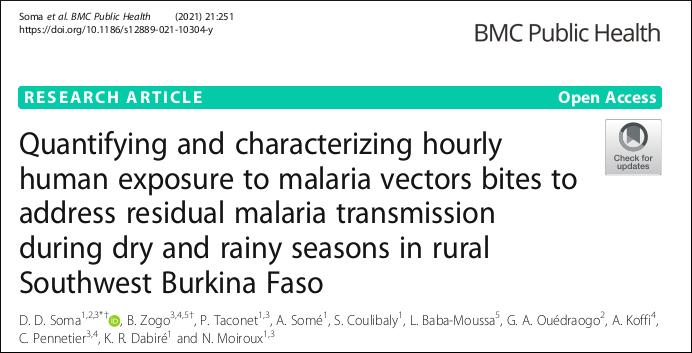
\includegraphics[width=1\linewidth]{figure/article0_couverture} 

}

\caption[Couverture de la publication n°3]{Couverture de la publication n°3}\label{fig:couv-art0}
\end{figure}
\hypertarget{summary-article-1}{%
\subsection{Résumé de l'article}\label{summary-article-1}}

Cette étude avait pour objectif de caractériser et quantifier la transmission résiduelle dans la zone d'étude de Diébougou (avant la mise en place de l'intervention dans le cadre de l'ERC) : mesurer le taux de protection conféré par les MIILDA, caractériser les sites et horaires où la population humaine est exposée à la piqûre d'anophèle, mesurer l'hétérogénéité spatio-temporelle de l'exposition au sein de la zone.\\

Nous avons utilisé une méthode permettant l'étude des intéractions comportementales entre les moustiques et les humains, décrite par Gerry F. Killeen et al. (\protect\hyperlink{ref-killeen_quantifying_2006}{2006}) puis améliorée par Geissbühler et al. (\protect\hyperlink{ref-geissbuhler_interdependence_2007}{2007}). Cette approche mathématique consiste à croiser des données de comportements nocturnes horaires des anophèles (densités agressives horaires à l'intérieur et à l'extérieur des habitations) et des personnes (horaires d'entrée et sortie des habitations, horaires de sommeil et utilisation ou non de moustiquaire). En sortie, les modèles procurent des informations sur l'exposition des humains aux piqûres d'anophèles, à chaque heure de la nuit. Nous avons ainsi utilisé les données horaires de comportement humain\footnote{issues des enquêtes de comportement humain relatif à l'utilisation des moustiquaires et aux habitudes horaires nocturnes, voir annexe \ref{humbehav-data}} et d'agressivité des anophèles collectées dans la zone de Diébougou en entrée de ce modèle mathématique. Nous avons stratifié l'étude par village, saison et classe d'âge de la population, afin d'affiner la connaissance sur les populations les plus à risque et les éventuelles hétérogénéités spatio-temporelles de l'exposition à la piqûre. Nous avons finalement judicieusement agrégé les sorties des modèles pour calculer les indicateurs de transmission résiduelle suivants :
\begin{itemize}
\tightlist
\item
  efficacité moyenne réelle de la protection personnelle offerte par l'utilisation d'une MIILDA (proportion de l'exposition aux piqûres qui est évitée par l'utilisation d'une MIILDA),
\item
  proportion de l'exposition se produisant à l'intérieur des habitations,
\item
  proportion de l'exposition se produisant avant 20 h ou après 5 h, correspondant aux horaires respectivement précédant et succédant les périodes ou la majorité (\textgreater{} 50 \%) des utilisateurs de MIILDA sont protégés.\\
\end{itemize}
Le taux moyen déclaré d'utilisation des MIILDA était très élevé, quelle que soit la saison ou la tranche d'âge (minimum : 92.45\% pour les + de 18 ans en saison sèche-chaude ; maximum : 100\% pour les 0 à 5 ans en saison pluvieuse). Nous avons noté de légères variations dans les taux d'utilisation des MIILDA selon les saisons (taux légèrement inférieurs en saison sèche par rapport à la saison humide), les tranches d'âge (taux légèrement inférieurs chez les adultes par rapport aux enfants), et les villages.
Les populations humaines étaient exposées quasiment exclusivement à l'intérieur de leurs habitations (94 \% de l'exposition se déroulait en intérieur); cependant, les MIILDA protégaient très efficacement de cette exposition (efficacité moyenne réelle comprise entre 80\% et 85\% selon les saisons). Le pic d'exposition résiduelle avait lieu à l'intérieur entre 5h et 6h du matin (33\% à 57\% de l'exposition résiduelle pour les utilisateurs de MIILDA), entre la sortie de l'espace de sommeil protégé par la moustiquaire et la sortie de l'habitation. Les piqûres précoces (avant 20h) représentaient moins de 12\% de l'exposition résiduelle.\\
\begin{figure}

{\centering 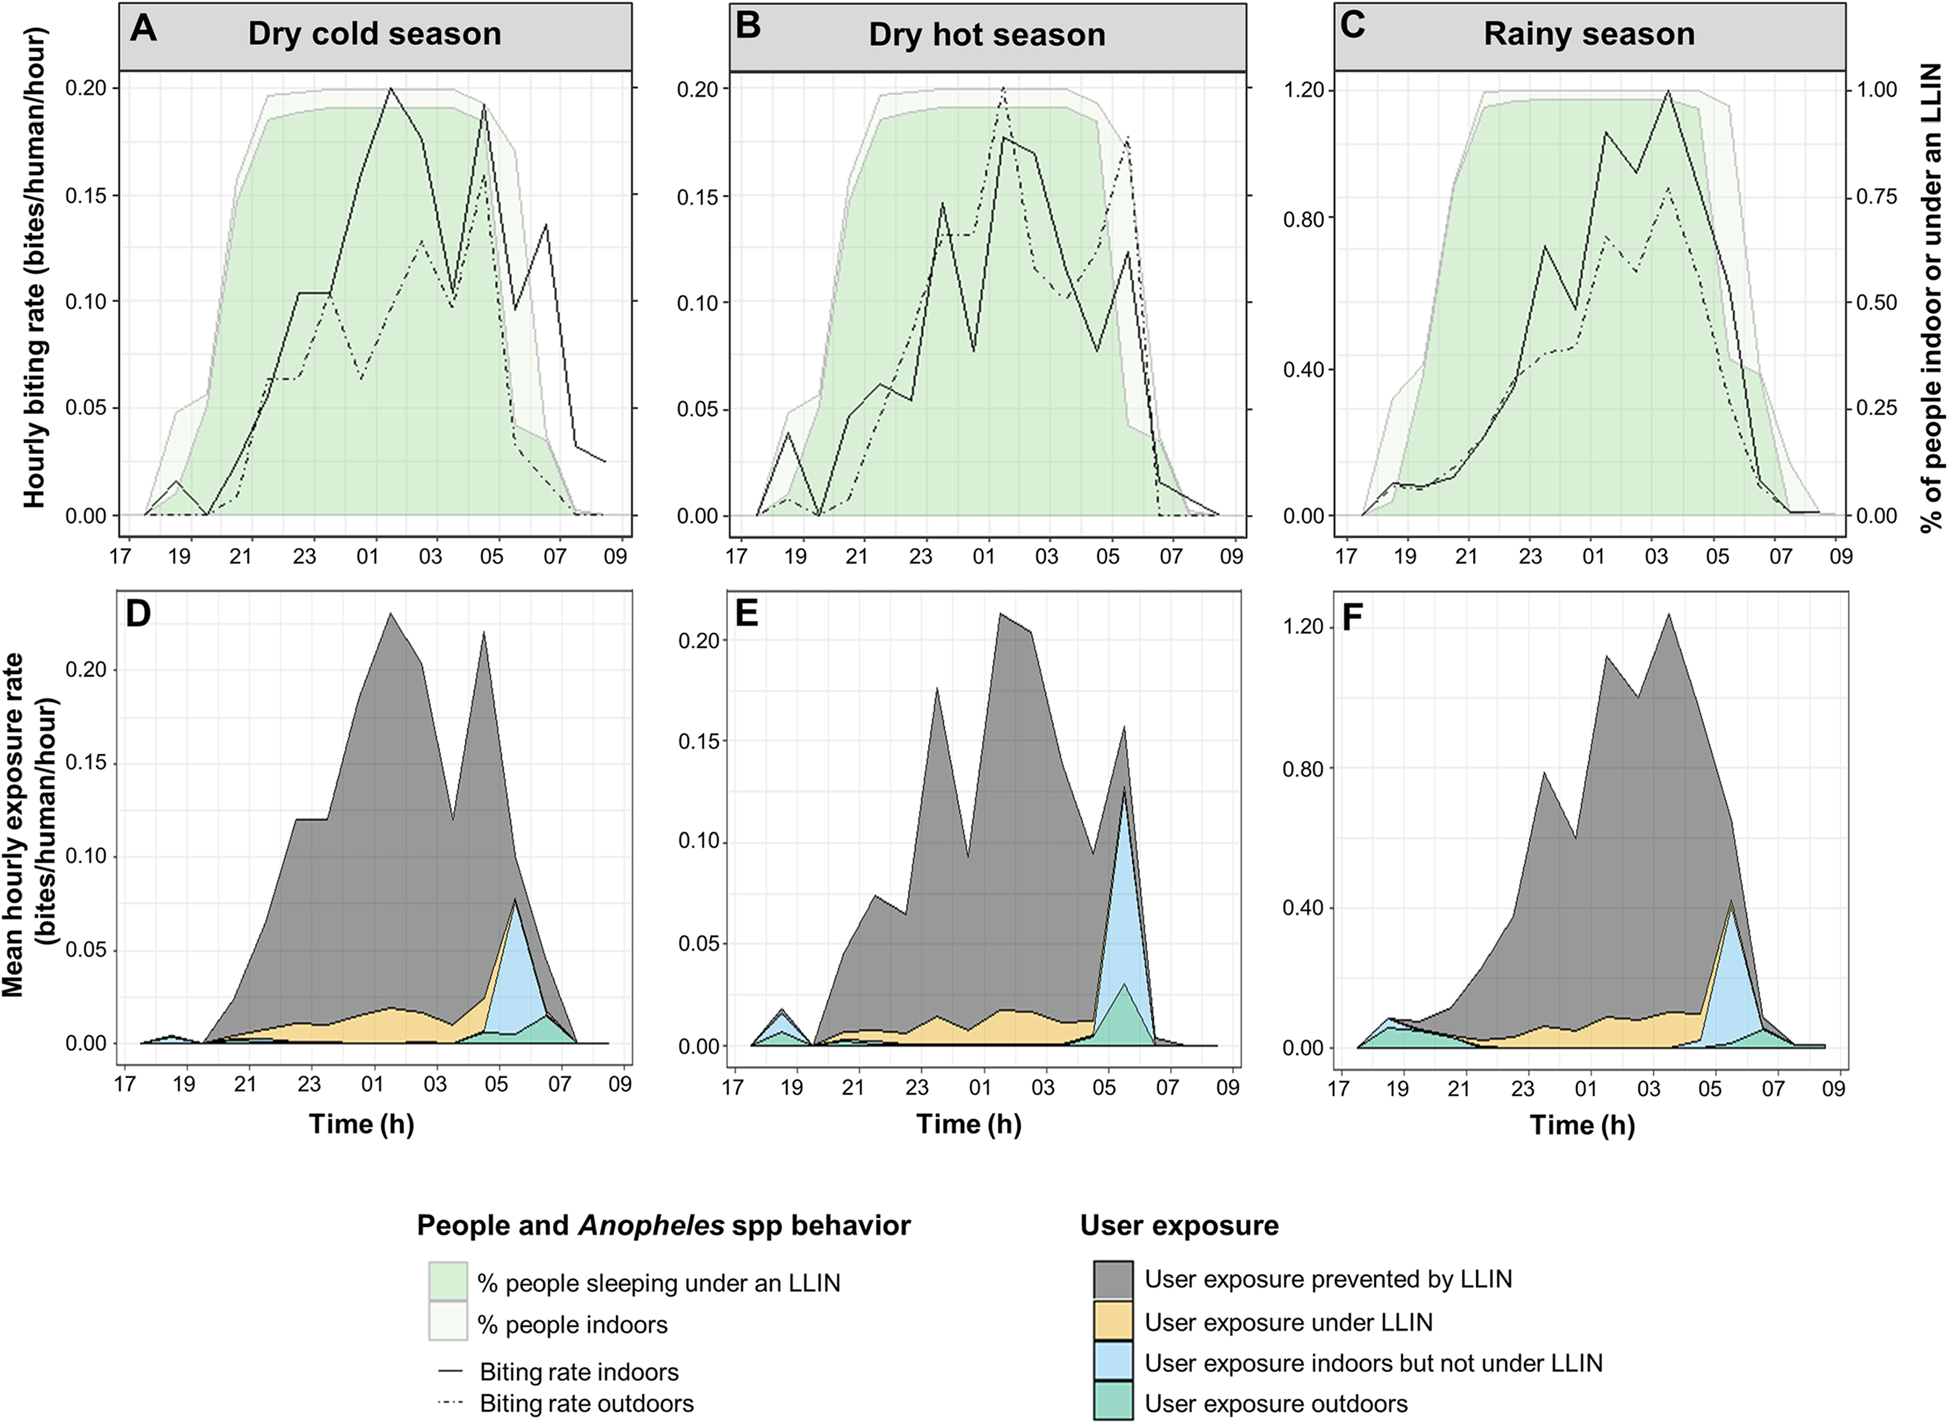
\includegraphics[width=.9\linewidth]{figure/human_exposure_bf} 

}

\caption[Comportement horaire humain et anophélien et exposition humaine horaire aux piqûres des utilisateurs de MIILDA]{Comportement horaire humain et anophélien (A, B, C) et exposition humaine horaire aux piqûres des utilisateurs de MIILDA (D, E, F)}\label{fig:human-exposure-bf}
\end{figure}
Cette étude a mis en évidence l'importance des MIILDA dans la lutte contre la transmission du paludisme dans la zone de Diébougou. Elle a notamment montré que les populations les plus à risque (enfants de moins de 5 ans) étaient aussi les plus protégées. Les taux déclarés d'utilisation des MIILDA étaient supérieurs à ceux rapportés par l'OMS, ce qui pourrait être dû au fait que les enquêtes de comportement humain ont été effectuées peu de temps après la dernière distribution universelle de moustiquaires. L'exposition résiduelle à la piqûre d'anophèle s'effectuant en majorité à l'intérieur des habitations, les outils ou mesures de LAV complémentaires devraient cibler prioritairement les vecteurs endophages (mesures telles que peintures insecticides, fermeture des avant-toits, fermeture des plafonds, ou encore grillage/moustiquaires aux fenêtres).\\

Dans la zone de Diébougou, les MIILDA protègent à priori considérablement des piqûres des vecteurs du paludisme. Cependant, les utilisateurs de moustiquaires restent exposés principalement à l'intérieur de leurs habitations, le matin. Aussi, la combinaison MIILDA + outil complémentaire de LAV visant les vecteurs endophages est probablement la plus efficace pour lutter contre la transmission résiduelle du paludisme dans cette zone.

\hypertarget{article-n4---moduxe9lisation-des-dynamiques-spatio-temporelles-des-cas-de-paludisme}{%
\section{Article n°4 - Modélisation des dynamiques spatio-temporelles des cas de paludisme}\label{article-n4---moduxe9lisation-des-dynamiques-spatio-temporelles-des-cas-de-paludisme}}

\hypertarget{introduction-uxe0-larticle-1}{%
\subsubsection{Introduction à l'article}\label{introduction-uxe0-larticle-1}}

Les travaux des chapitres 4 et 5 ont montré comment les images satellitaires et les modèles statistiques peuvent aider à comprendre et prédire les dynamiques entomologiques spatio-temporelles sur nos territoires d'étude ; ces éléments permettant d'optimiser la conception et le déploiement des outils de LAV. Mais ces mêmes outils peuvent également être utilisés en épidémiologie, pour expliquer ou prédire la distribution spatio-temporelle d'indicateurs épidémiologiques tels que la prévalence du paludisme. Une telle prédiction permet alors d'optimiser le déploiement de mesures de prévention, diagnostic et de traitement de la maladie. Dans cette dernière étude, nous avons étudié les dynamiques spatio-temporelles des cas de paludisme dans la zone de Diébougou. Nous montrons i) que la distribution spatiale des cas de paludisme est hétérogènes au sein du district sanitaire ; et ii) que nous pouvons y anticiper les pics épidémiques plusieurs semaines à l'avance grâce aux données satellitaires et aux modèles statistiques. Cette étude a fait l'objet d'une publication scientifique, que nous résumons ci-dessous. Le texte intégral est disponible en annexe \ref{full-article-bationo} et à l'adresse suivante : \url{https://doi.org/10.1038/s41598-021-99457-9}.\\
\begin{figure}

{\centering 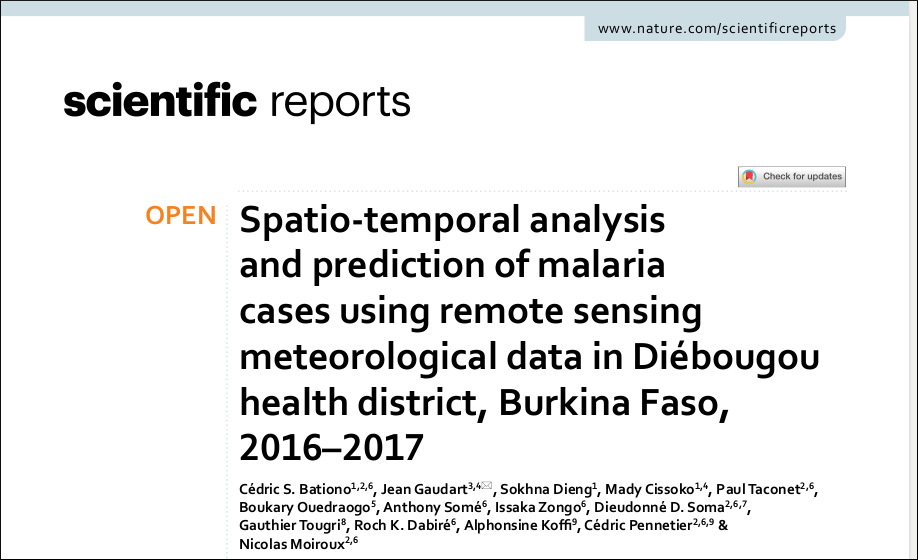
\includegraphics[width=1\linewidth]{figure/article2_couverture} 

}

\caption[Couverture de la publication n°4]{Couverture de la publication n°4}\label{fig:couv-art2}
\end{figure}
\hypertarget{ruxe9sumuxe9-de-larticle-1}{%
\subsection{Résumé de l'article}\label{ruxe9sumuxe9-de-larticle-1}}

Les objectifs de cette étude étaient i) d'étudier la dynamique spatiale de l'épidémiologie du paludisme dans la zone de Diébougou, en détectant d'éventuels `points chauds' spatiaux de cas de paludisme et ii) de modéliser les dynamiques temporelles des cas de paludisme dans la zone d'étude en utilisant des données météorologiques satellitaires, afin d'appréhender la capacité à anticiper les épidémies de la maladie dans le district sanitaire.\\

Les données hebdomadaires de cas de paludisme en 2016 et 2017 ont été collectées dans 13 centres de santé de la zone. Les points chauds spatiaux de cas de paludisme ont été détectés en utilisant des méthodes d'analyse statistique spatiale. Les cas reportés de paludisme ont été comparés à la distance euclidienne du village au centre de santé et à la densité agressive des vecteurs afin de tenter d'expliquer les différences observées entre les villages. Pour l'analyse temporelle, les données météorologiques ont été extraites de produits satellitaires ou issues de modèles météorologiques, disponibles à l'échelle mondiale. Ces données sont produites en routine par le Centre Européen pour les Prévisions Météorologiques à Moyen Terme. Deux variables statistiques synthétisant les données météorologiques à l'échelle hebdomadaire (\emph{Synthetic Meteorological Indicator} ou SMI) ont été construites par analyse en composantes principales. Dans une première analyse bivariée, des modèles additifs généralisés (\emph{Generalized Additive Model} ou GAM) ont été entrainés pour modéliser le nombre de cas de paludisme à l'échelle de la zone d'étude entière et au pas de temps hebdomadaire en fonction de chacune des deux variables météorologiques, utilisées tour à tour sur chacune des 30 semaines précédant les cas de paludisme à expliquer/prédire. Les variables dont les `lags' temporels conduisaient à la plus petite erreur dans ces analyses bivariées ont ensuite été utilisées en tant que variables indépendantes dans un GAM mixte multivarié, entrainé sur les données d'une année entière. La capacité prédictive de ce modèle multivarié a finalement été évaluée en prédisant le nombre de cas de paludisme sur une période de 17 semaines non utilisées pour entrainer le modèle (correspondant au pic épidémique suivant, en 2017) et en évaluant graphiquement la superposition des courbes épidémiologiques observées et prédites par le modèle statistique.\\

Nous avons observé que la distribution des cas de paludisme était hétérogène à l'échelle du district sanitaire, à la fois spatialement et temporellement. Quatre points chauds spatiaux ont été identifiés, regroupant chacun entre un et trois villages (figure \ref{fig:map-malaria-cases}). La distribution spatiale des cas de paludisme n'était corrélée ni à la distance euclidienne au centre de santé, ni aux densités agressives des anophèles. Aussi, l'hétérogénéité spatiale de la densité des vecteurs n'explique à priori pas, dans cette zone, celle de la prévalence des cas. Pour l'accès aux centres de santé, des variables plus réalistes pourraient être testées (par exemple, distance réelle au centre, ou encore accessibilité pendant la saison pluvieuse). D'autres facteurs, restants à explorer, pourraient expliquer l'hétérogénéité spatiale des cas de paludisme dans notre zone (différences dans les niveaux d'éducation, revenus, activités profesionnelles, possession et utilisation des MIILDA, etc.).\\
\begin{figure}

{\centering \includegraphics[width=0.9\linewidth]{figure/map_malaria_cases} 

}

\caption[Distribution spatiale des cas de paludisme reportés dans les 27 villages de la zone de Diébougou pour l'année épidémique 2016-2017]{Distribution spatiale des cas de paludisme reportés dans les 27 villages de la zone de Diébougou pour l'année épidémique 2016-2017. Les cercles rouges représentent les point chauds}\label{fig:map-malaria-cases}
\end{figure}
Au niveau temporel, un pic épidémique a été relevé entre les mois d'août et novembre 2016. Les SMI présentant les meilleurs capacités prédictives (c.a.d. les plus faibles erreurs) étaient situés respectivement 9 et 16 semaines avant les cas prédits, pour chacun des deux SMI. Le modèle multivarié généré avec ces deux SMI prédisait correctement le départ de la prochaine épidémie, 9 semaines à l'avance, avec cependant un décalage (retard) de 3 semaines environ sur la courbe épidémiologique prédite (figure \ref{fig:prediction-malaria-cases}).\\
\begin{figure}

{\centering \includegraphics[width=1\linewidth]{figure/prediction_malaria_cases} 

}

\caption[Nombre cumulé de cas reportés et prédits par le modèle statistique basé sur des données météorologiques dans les 27 villages de la zone de Diébougou]{Nombre cumulé de cas reportés (courbe noire) et prédits par le modèle statistique basé sur des données météorologiques (courbe orange) dans les 27 villages de la zone de Diébougou}\label{fig:prediction-malaria-cases}
\end{figure}
Cette étude a ainsi montré que la distribution spatio-temporelle des cas de paludisme était hétérogène à l'échelle du district sanitaire, justifiant ainsi de cibler les interventions de prévention, diagnostic, et traitement. Nous avons également montré qu'il est possible d'anticiper la prévalence du paludisme plusieurs semaines à l'avance dans la zone de Diébougou grâce aux données météorologiques issues des images satellitaires et aux modèles statistiques. Ces données et méthodes pourraient être utilisées pour mettre en place un système d'alerte précoce qui identifierait les zones (villages ou points chauds) et périodes prioritaires pour les campagnes de lutte contre le paludisme. Un tel système d'alerte précoce gagnerait à être alimenté en continu par les données épidémiologiques des centres de santé, afin d'améliorer les prédictions.

\begingroup 
\renewcommand{\headrulewidth}{0pt}

\markboth{}{}

\includepdf[pages=3,nup=1,pagecommand={}]{pagesgarde.pdf}
\endgroup

\hypertarget{discussion}{%
\chapter{Discussion générale}\label{discussion}}

Après d'importants progrès, la morbidité et la mortalité liées au paludisme dans le monde ne recule plus -- voire ré-augmente. Redynamiser le progrès nécessite de repenser certaines approches, entre autres~: élargir la palette d'outils de lutte contre la transmission, déployer des interventions adaptées au contexte local, prioriser leur déploiement. Dans cette optique, la recherche scientifique se doit de proposer, concevoir, et tester de nouvelles stratégies et outils pour la surveillance et le contrôle du paludisme. Ces propositions doivent être construites sur la base d'une connaissance fine et localisée du risque de transmission du paludisme.\\

Dans ce cadre, cette thèse avait pour objectif principal d'approfondir les connaissances sur le risque de transmission résiduelle du paludisme -- à savoir, la probabilité de contact homme-vecteur - dans deux zones d'étude d'environ 50 km x 50 km, en milieu rural ouest-africain, en implémentant, en partie, trois approches~: mesurer et caractériser le risque, comprendre le risque, prédire le risque. Pour ce faire, nous avons étudié certains indicateurs entomologiques du risque de transmission en utilisant des méthodes de modélisation statistique descriptives et prédictives. Nous nous sommes intéressés en particulier à la bio-écologie des vecteurs du paludisme~: déterminants et prédictibilité spatio-temporelle de leur probabilité de présence, de leur abondance, de leurs résistances physiologiques, et de leurs résistances comportementales.\\

Basé sur les résultats et limites des travaux de thèse, ce dernier chapitre est une discussion principalement constituée de propositions, axes de recherche ou opérationnels, pour la recherche et le contrôle du paludisme dans nos zones d'étude et au-delà. Cette discussion est composée de deux grandes parties. La première partie est une discussion traitant d'entomologie médicale pour la prévention du paludisme. En nous appuyant sur les résultats de la thèse, nous définissons tout d'abord un ensemble de caractéristiques générales pour améliorer la LAV dans nos zones d'étude, décrivons ou mentionnons brièvement quelques outils de LAV existants répondant à ces caractéristiques, et présentons quelques limites de la thèse et perspectives de recherche qui permettraient d'améliorer la définition de ces caractéristiques. La deuxième partie de la discussion est davantage méthodologique et orientée autour de la science des données pour l'entomologie médicale et la géo-épidémiologie. En nous appuyant sur les travaux de la thèse et certaines réflexions ou observations personnelles, nous proposons dans un premier temps quelques pistes pour mieux exploiter le potentiel offert par la science et l'ingénierie des données dans la recherche en entomologie médicale et en géo-épidémiologie du paludisme. Dans un deuxième temps et pour terminer la discussion, nous définissons les contours d'un outil de surveillance et prévention du paludisme qui pourrait être développé au regard des résultats de la thèse pour nos zones d'étude et au-delà, pour le milieu rural ouest-africain.

\hypertarget{propositions-pour-des-stratuxe9gies-de-ruxe9duction-du-risque-de-transmission-ruxe9siduelle-sur-nos-zones-duxe9tude}{%
\section{Propositions pour des stratégies de réduction du risque de transmission résiduelle sur nos zones d'étude}\label{propositions-pour-des-stratuxe9gies-de-ruxe9duction-du-risque-de-transmission-ruxe9siduelle-sur-nos-zones-duxe9tude}}

\hypertarget{duxe9finition-des-caractuxe9ristiques-de-la-lav-et-stratuxe9gies-potentielles-concruxe8tes}{%
\subsection{Définition des caractéristiques de la LAV et stratégies potentielles concrètes}\label{duxe9finition-des-caractuxe9ristiques-de-la-lav-et-stratuxe9gies-potentielles-concruxe8tes}}

La portée opérationnelle de ces recherches est la conception et le déploiement optimisé de mesures de LAV durables et adaptées au faciès local. Sur la base des résultats de nos travaux de recherche, nous proposons ici quelques pistes pour une LAV plus efficace sur nos deux zones d'étude.\\

\textgreater{} \textbf{\emph{Dans les deux zones, conserver la moustiquaire comme outil de base et principal de la lutte anti-vectorielle.}} Notre travail supporte, s'il en est encore besoin, la moustiquaire, distribuée universellement, comme outil premier et fondamental de la LAV : dans la zone de Diébougou, nous avons mesuré que les moustiquaires protégeaient leurs utilisateurs, grâce à leur effet barrière, de plus de 80\% des piqûres potentielles d'anophèles. Bien que la méthode utilisée (enquêtes déclaratives) puisse avoir tendance à sur-évaluer les taux d'utilisation réels, ces ordres de grandeur confirment l'importance de cet outil dans la lutte contre la transmission du paludisme. Il serait opportun de réaliser une étude similaire dans la zone de Korhogo avec les données du projet REACT.\\

\emph{Concrètement~:} Il apparaît essentiel de maintenir l'effort de distribution universelle des moustiquaires, tels que le font le Burkina Faso et la Côte d'Ivoire depuis 12 années maintenant. La question de l'imprégnation des moustiquaires par les insecticides, davantage discutable, fait l'objet d'un paragraphe à suivre. Par ailleurs, la fréquence optimale de distribution des moustiquaires, aujourd'hui de 3 à 4 ans dans les deux pays, reste à évaluer. L'OMS estime à trois ans la durée de conservation des moustiquaires (\protect\hyperlink{ref-10665-69986}{WHO, 2009}), mais certaines études montrent qu'elle pourrait être bien inférieure (\protect\hyperlink{ref-bertozzi-villa_maps_2021}{Bertozzi-Villa et al., 2021}).\\

\textgreater{} \textbf{\emph{Dans les deux zones, déployer urgemment des stratégies de LAV complémentaires à la MIILDA.}} Nous avons observé que les densités agressives des vecteurs sur nos zones d'étude étaient élevées (en particulier dans la zone de Korhogo), avec en moyenne, sur la durée du projet, 2,0 piqûres/homme/nuit à Diébougou et 28,2 piqûres/homme/nuit à Korhogo . Les données recueillies dans le cadre du projet REACT ont montré un taux d'inoculation entomologique (nombre de piqûres infectieuses/homme/an) de 898 dans la zone de Korhogo (\protect\hyperlink{ref-zogo_anopheles_2019}{Zogo, Soma, et al., 2019}) et d'environ 100 dans la zone de Diébougou (\protect\hyperlink{ref-soma_anopheles_2020}{Soma et al., 2020}), plaçant ces zones au dessus de la moyenne africaine en ce qui concerne le risque de transmission du paludisme (\protect\hyperlink{ref-gething_new_2011}{Gething et al., 2011}; \protect\hyperlink{ref-killeen_short_1999}{G. F. Killeen, Githure, \& Beier, 1999}). Ces indicateurs particulièrement élevés montrent que la moustiquaire, bien qu'essentielle, doit très probablement être complémentée d'autres stratégies de LAV pour prévenir la transmission du paludisme.\\

\emph{Concrètement~:} La recherche, le développement et l'évaluation de nouveaux outils de LAV sont des secteurs actifs (\protect\hyperlink{ref-barreaux_priorities_2017}{Barreaux et al., 2017}, ~; \protect\hyperlink{ref-killeen_characterizing_2014}{Gerry F. Killeen, 2014}; \protect\hyperlink{ref-sougoufara_need_2020}{Seynabou Sougoufara, Ottih, \& Tripet, 2020}; \protect\hyperlink{ref-who_2017_who_nodate}{WHO, 2017b}; \protect\hyperlink{ref-wilson_importance_2020}{Wilson et al., 2020}). Les outils actuellement développés ou testés sont très variés, ciblant une vaste gamme de stades de vie des vecteurs et de leurs comportements~; et vont du conceptuellement très simple (amélioration des habitations) au technologiquement complexe (modifications génétiques). Pour ne mentionner que quelques-unes de ces stratégies, citons~: la lutte anti-larvaire (à base de bio-larvicides ou d'espèces prédatrices), la lutte génétique (techniques de l'insecte stérile et de l'insecte incompatible, forçage génétique), la protection personnelle (répulsifs cutanés, serpentins fumigènes, etc.), l'aménagement du territoire (drainage des eaux de surface, etc.), l'administration d'endectocides, les pulvérisations spatiales d'insecticide à l'extérieur des habitations, etc. Il s'agit d'autant de stratégies qui pourraient être envisagées pour réduire le risque de transmission sur nos zones d'étude.\\

\textgreater{} \textbf{\emph{À Diébougou, déployer des stratégies complémentaires à la MIILDA ciblant spécifiquement les vecteurs endophages et endophiles.}} En caractérisant le risque de contact homme-vecteur dans la zone de Diébougou, nous avons mis en évidence que les populations restaient exposées à la piqûre d'anophèle, principalement le matin à l'intérieur des habitations. Aussi, dans cette zone au moins, il apparaît nécessaire de déployer également des outils complémentaires ciblant les vecteurs endophages pour réduire le risque de transmission.\\

\emph{Concrètement~:} Afin de cibler spécifiquement les vecteurs endophages ou endophiles, en sus des stratégies citées précédemment et des PID, des mesures relativement simples ayant pour objectif d'améliorer les habitations pour réduire l'entrée des vecteurs par des barrières physiques pourraient être déployées : la fermeture des avants-toits, les grillages sur les fenêtres et les portes, les tubes d'avant-toits, etc. (\protect\hyperlink{ref-animut_impact_2013}{Animut, Balkew, \& Lindtjørn, 2013}; \protect\hyperlink{ref-atieli_house_2009}{Atieli, Menya, Githeko, \& Scott, 2009}; \protect\hyperlink{ref-bradley_reduced_2013}{Bradley et al., 2013}, ~; \protect\hyperlink{ref-sternberg_eave_2016}{Sternberg et al., 2016}; \protect\hyperlink{ref-ye_housing_2006}{Yé et al., 2006}). Des mesures telles que l'optimisation de l'utilisation des MIILDA peuvent également avoir un impact positif. Par exemple, dans le cadre du projet REACT, la stratégie d'IEC déployée en complément des MIILDA (voir section \ref{study-areas}) a significativement réduit la morbidité de la maladie sur les deux zones d'étude par rapport aux MIILDA seules (Moiroux 2021, soutenance d'Habilitation à Diriger des Recherches).\\

\textgreater{} \textbf{\emph{Dans les deux zones, déployer des stratégies complémentaires à la MIILDA ciblant spécifiquement les vecteurs exophages.}} L'étude des comportements trophiques des anophèles a mis en évidence un niveau d'exophagie moyen important dans les deux zones (41 \% à Diébougou, 56 \% à Korhogo). Ces vecteurs ne sont pas ciblés par les outils actuellement utilisés (MIILDA principalement). Aussi, il semble nécessaire, pour réduire le risque de transmission, de déployer des outils ciblant ces vecteurs qui piquent à l'extérieur. Nous avons également observé que les proportions de vecteurs exophages étaient relativement homogènes spatio-temporellement au sein de chaque district sanitaire, et avons émis l'hypothèse que les conditions environnementales (autres que celles liées à l'utilisation des insecticides) n'impactaient que marginalement le comportement trophique des vecteurs. Il n'y aurait ainsi probablement pas de bénéfice particulier à adapter la lutte spécifique contre les vecteurs exophages au village ou à la saison. Notons, cependant, que cela n'implique pas qu'il n'y ait pas de bénéfice à prioriser les villages et/ou saisons dans lesquels ces outils seront déployés, si les ressources sont limitées.\\

\emph{Concrètement~:} En plus de toutes les stratégies précédemment citées (qui visent indistinctement les vecteurs exophages / exophiles et endophages / endophiles), une des stratégies existantes et déployables à l'extérieur (mais aussi à l'intérieur) des habitations consiste à piéger les vecteurs à l'aide d'appâts sucrés (\emph{Attractive Toxic Sugar Baits}). Ces pièges relativement simples contiennent du sucre (alimentation des moustiques mâles et femelles) et des substances toxiques qui sont sélectives et qui ont des effets minimes sur les espèces non ciblées et sur l'environnement (\protect\hyperlink{ref-beier_attractive_2012}{Beier, Müller, Gu, Arheart, \& Schlein, 2012}; \protect\hyperlink{ref-muller_successful_2010}{Müller et al., 2010}; \protect\hyperlink{ref-stewart_indoor_2013}{Stewart et al., 2013}).\\

\textgreater{} \textbf{\emph{Dans les deux zones, modifier l'usage des insecticides dans la LAV.}} Dans les deux zones d'étude, nous avons observé que les vecteurs étaient en mesure de résister efficacement aux effets létaux des insecticides : en évitant ou en contournant leurs effets létaux. Nous avons émis l'hypothèse que ces résistances, qu'elles soient physiologiques ou comportementales, continuaient à se développer dans les zones d'étude et qu'elles étaient principalement causées par les insecticides utilisés dans la LAV. Ces constats appellent à repenser l'utilisation des insecticides dans la LAV sur nos zones d'étude.\\

\emph{Concrètement~:} Différentes pistes sont~envisageables, citons par exemple (\protect\hyperlink{ref-paaijmans_taking_2020}{Paaijmans \& Huijben, 2020}; \protect\hyperlink{ref-organization_framework_2017}{WHO, 2017a}): la modification de la nature des insecticides, les mosaïques ou la rotation d'insecticides, l'utilisation des insecticides dans des outils alternatifs aux MIILDA, ou encore le retrait pur et simple des insecticides de la boite à outils des mesures de LAV. Depuis la tenue du projet REACT, le Burkina Faso et la Côte d'Ivoire ont implémenté de nouvelles stratégies d'utilisation des insecticides. En effet, lors de la distribution universelle de 2019, le Burkina Faso a distribué des moustiquaires imprégnées d'un mélange pyréthrinoïdes - piperonyl butoxide (PBO), dont l'efficacité épidémiologique et entomologique par rapport aux moustiquaires imprégnées de pyréthrinoïdes uniquement a été démontrée en zone de forte résistance des vecteurs aux insecticides -- et notamment au Burkina Faso (\protect\hyperlink{ref-gleave_2021}{Gleave, Lissenden, Chaplin, Choi, \& Ranson, 2021}). La Côte d'Ivoire a, de son côté, stratifié la distribution des moustiquaires en 2021 selon quatre zones en fonction des informations disponibles sur les résistances physiologiques des vecteurs dans le pays. Un suivi des indicateurs entomologiques et épidémiologiques sur le long terme semble essentiel pour évaluer l'efficacité de ces nouvelles stratégies.\\

\textgreater{} \textbf{\emph{Dans les deux zones, cibler et prioriser le déploiement des stratégies complémentaires à la MIILDA.}} Nous avons observé dans les deux zones que la distribution des populations de vecteurs était fortement hétérogène temporellement (entre les saisons) -- comme l'on pouvait s'y attendre -- mais aussi spatialement (entre les villages). Aussi, il y aurait très probablement un bénéfice à cibler les mesures de LAV complémentaires à l'échelle de la saison et du village, ainsi que prioriser leur déploiement si les ressources sont limitées. Par ailleurs, nous avons identifié nombre de déterminants de la probabilité de présence et de l'abondance des vecteurs - autant d'informations permettant d'identifier les leviers d'action les plus pertinents pour lutter localement contre les vecteurs.\\

\emph{Concrètement~:} Des outils de surveillance et de prédiction spatio-temporelle du risque de transmission, tels que des cartes ou des systèmes d'alerte précoces, pourraient être développés (ce point spécifique fait l'objet de la section \ref{surveillance-prevention-tools} en fin de discussion). De tels outils de surveillance permettent d'envisager une LAV ciblée et priorisée dans l'espace et dans le temps. En effet, les cartes saisonnières de la distribution spatiale des densités agressives des vecteurs pourraient permettre de cibler ou prioriser le déploiement de mesures ponctuelles (amélioration des habitations, aménagement de l'environnement, etc.) ou nécessitant une certaine récurrence (lutte anti-larvaire, IEC, etc.). Les systèmes d'alerte précoce, de leur côté, pourraient permettre de déployer des mesures préventives exceptionnelles (campagnes de larvicides, alertes à la population, etc.) dans les villages et moments pour lesquels un seuil de risque (à définir) est franchi. L'ensemble des procédures liées à la LAV (nature des interventions, sites et fréquences de de déploiement, cartes, seuils d'alerte de risque et interventions à déployer, etc.) gagneraient à être décrites dans des plans de gestion de LAV ad hoc.

\hypertarget{principales-limites-et-perspectives-de-recherche}{%
\subsection{Principales limites et perspectives de recherche}\label{principales-limites-et-perspectives-de-recherche}}

Bien que la thèse ait permis de définir certaines caractéristiques pour la LAV sur nos zones d'étude, de nombreuses questions -- dont les réponses permettraient d'améliorer la définition de ces caractéristiques - restent en suspens. Nous exposons ci-dessous quelques-unes des limites de la thèse et perspectives de recherche associées.\\

\textgreater{} \textbf{\emph{Tester, de manière expérimentale, les hypothèses soulevées dans les travaux de modélisation descriptive holistico-inductive.}} Les travaux de la thèse ont soulevé un certain nombre d'hypothèses ou de questions de recherche. Par exemple : À quoi sont dues les corrélations fortes entre les densités agressives des vecteurs et les variables météorologiques précédant la durée de vie des moustiques capturés ( \textgreater{} 3 semaines avant)~: dynamiques de population~, effets paternels / maternels , ou préparation de conditions biotiques ou abiotiques favorables ? Quelle est l'explication biologique de l'association positive entre le niveau d'ouverture du paysage et les densités agressives ? Pour ces mêmes associations, les seuils révélés par les modèles sont-ils liés à un biais d'échantillonnage ou représentent-ils une réalité biologique~? Dans le même ordre d'idée, les associations entre la prévalence des résistances comportementales des vecteurs et la météorologie au cours du mois précédant les captures entomologiques sont-elles une réalité biologique (coût de mutations liées à un caractère éventuellement héréditaire des résistances comportementales) ou bien un biais d'échantillonnage~? Puisque les variables introduites dans les modèles de résistance n'expliquaient que peu la probabilité de résistance comportementale des vecteurs, quels sont les autres déterminants des résistances comportementales des vecteurs (génétique, hasard) ? Puisqu'à l'échelle du district sanitaire, la prévalence des résistances est globalement stable dans l'espace et dans le temps, à quelle(s) échelle(s) fluctuent, de manière significative, les dynamiques spatiales et temporelles des résistances des vecteurs ? Ces diverses questions et hypothèses pourraient être étudiées et testées expérimentalement, dans des approches hypothético-déductives réductionnistes.\\

\textgreater{} \textbf{\emph{Expliquer et prédire les composantes du risque de transmission résiduelle non étudiées dans la thèse (possession et utilisation des moustiquaires, niche d'activité des vecteurs).}} Dans cette thèse, nous n'avons étudié qu'une partie des composantes du risque de transmission résiduelle (en l'occurrence~: présence, abondances, et résistances des vecteurs) identifiés dans le chapitre 1 (voir section \ref{explain-risk}). Pour compléter la définition des caractéristiques des outils de LAV complémentaires et cibler ou prioriser leur déploiement, il serait important d'expliquer et de prédire d'autres composantes du risque de transmission résiduelle, liées à l'homme ou au vecteur. En particulier, il serait intéressant d'étudier les déterminants de la possession, utilisation, et horaires d'utilisation des moustiquaires~; ainsi que ceux des horaires d'activité de recherche de repas du sang («~niche d'activité~») des vecteurs. Les conditions et horaires d'utilisation (ou absence d'utilisation) des moustiquaires peuvent être modulées par de nombreux facteurs socio-culturels, environnementaux, climatiques, entomologiques (\protect\hyperlink{ref-monroe_measuring_2019}{Monroe, Moore, Koenker, Lynch, \& Ricotta, 2019}, ~; \protect\hyperlink{ref-koenker_2019}{Koenker et al., 2019}). La niche d'activité du vecteur, quand à elle, reste peu étudiée, et pourrait être contrainte - entre autres -- par les conditions micro-climatiques (\protect\hyperlink{ref-yin_field-based_2019}{Yin et al., 2019}). Les données du projet REACT (de terrain et satellitaires) et les approches de modélisation statistique utilisées dans cette thèse pourraient être utilisées pour étudier ces composantes du risque.\\

\textgreater{} \textbf{\emph{Tester l'efficacité des moustiquaires sans insecticides.}} Parmi les stratégies de gestion des résistances des vecteurs aux insecticides, la moustiquaire sans insecticides est une approche qu'il serait intéressant de tester (\protect\hyperlink{ref-paaijmans_taking_2020}{Paaijmans \& Huijben, 2020}). La question qui se pose ici est celle de l'origine de la protection communautaire conférée par les moustiquaires. En effet, l'insecticide dont la moustiquaire est imprégnée a pour objectif principal de réduire la longévité des vecteurs, et donc la population globale de vecteurs, conférant finalement la protection communautaire (voir section \ref{lav-principaux-outils}). Cependant, la barrière physique que constitue la moustiquaire empêche le vecteur de se gorger de sang, bloquant ainsi son cycle biologique, et \emph{in fine} est également susceptible de réduire la densité globale des vecteurs. La mesure dans laquelle l'intensité de la transmission locale est réduite par la barrière chimique ou physique de la moustiquaire n'a pas été étudiée (\protect\hyperlink{ref-paaijmans_taking_2020}{Paaijmans \& Huijben, 2020}). Dans un contexte de fortes résistances aux insecticides -- où l'effet de la barrière chimique pourrait être perdu, voire pourrait avoir l'effet inverse à celui attendu (\emph{behavioural exploitation}) - il pourrait être intéressant de comparer expérimentalement l'efficacité de moustiquaires imprégnées et de moustiquaires non imprégnées d'insecticides. De telles moustiquaires auraient par ailleurs certains avantages non-négligeables par rapport aux moustiquaires imprégnées~: coût, durabilité, réduction des risques sur la santé humaine et sur l'environnement (\protect\hyperlink{ref-paaijmans_taking_2020}{Paaijmans \& Huijben, 2020}).\\

\textgreater{} \textbf{\emph{Quantifier l'impact épidémiologique des résistances des vecteurs aux insecticides.}} Enfin, la question de l'impact des résistances des vecteurs sur la transmission effective du paludisme, et plus globalement, de l'association entre entomologie et épidémiologie, reste à développer. De nombreuses questions restent ainsi en suspens, par exemple~: quel est l'impact des résistances des vecteurs (physiologiques, comportementales, ou leur interaction) sur l'épidémiologie du paludisme dans nos zones d'étude~? Les données entomologiques et épidémiologiques du projet REACT pourraient être croisées pour répondre à ces questions. Rappelons qu'à l'échelle de l'Afrique, le modèle mathématique utilisé par Sherrard-Smith et al. (\protect\hyperlink{ref-sherrard-smith_mosquito_2019}{2019}) prédisait que les résistances des vecteurs étaient susceptibles d'avoir un impact significatif sur la morbidité de la maladie (voir section \ref{behavioural-resistance}).

\hypertarget{propositions-pour-une-meilleure-exploitation-de-la-science-et-de-linguxe9nierie-des-donnuxe9es-pour-la-recherche-et-le-contruxf4le-du-paludisme}{%
\section{Propositions pour une meilleure exploitation de la science et de l'ingénierie des données pour la recherche et le contrôle du paludisme}\label{propositions-pour-une-meilleure-exploitation-de-la-science-et-de-linguxe9nierie-des-donnuxe9es-pour-la-recherche-et-le-contruxf4le-du-paludisme}}

\hypertarget{potentiel-data-science}{%
\subsection{Connaître et exploiter le potentiel de la science des données en entomologie médicale et géo-épidémiologie}\label{potentiel-data-science}}

Les travaux de cette thèse ont largement fait appel à des méthodes et outils de la science des données. Dans un monde toujours plus numérisé, dans lequel les données sont toujours plus abondantes, fines, accessibles, abordables, la recherche et la gestion du paludisme ne doit pas manquer les opportunités offertes par la science des données. Celles-ci sont nombreuses, et concernent des aspects à la fois de recherche et opérationnels. Cette thèse a montré comment l'utilisation judicieuse de données hétérogènes (spatio-temporelles, multi-source, multi-échelle) permet à la fois d'approfondir les connaissances et peut avoir une portée très opérationnelle, via le développement d'outils concrets de surveillance du risque de transmission. Dans cette section, nous discutons d'aspects méthodologiques -- là aussi sous forme de propositions -- liés à l'exploitation de la science et de l'ingénierie des données pour la recherche ou le contrôle du paludisme.\\

\textgreater{} \textbf{\emph{Connaître et exploiter pleinement le potentiel offert par la modélisation statistique.}} Comme nous l'avons expliqué dans le chapitre 2 et montré à travers les travaux de la thèse, aujourd'hui la modélisation statistique n'est plus seulement un outil de vérification d'hypothèse scientifique : c'est également un véritable outil à part entière de création de connaissances, d'hypothèses scientifiques. En effet, un modèle statistique peut capturer des associations inattendues pouvant soulever de nouvelles hypothèses qui peuvent ensuite être testées expérimentalement. Il semble aujourd'hui que la recherche dans des domaines tels que la géo-épidémiologie n'exploite pas encore pleinement son potentiel. Par exemple, une revue de littérature récente a montré que les modèles statistiques utilisés en géo-épidémiologie pour prédire la distribution spatio-temporelle de certaines grandes maladies vectorielles (paludisme, dengue, virus du Nil occidental) sont principalement des modèles paramétriques type GLMM (\protect\hyperlink{ref-parselia_satellite_2019}{Parselia et al., 2019}). À l'heure des modèles d'apprentissage automatique en capacité de capturer des associations complexes, des outils permettant d'interpréter ces modèles, et des données volumineuses, il semble nécessaire que les domaines de l'entomologie médicale et de la géo-épidémiologie prennent davantage conscience du potentiel offert par la modélisation statistique, à la fois pour la recherche afin de construire des hypothèses scientifiques à partir des données, et pour la gestion afin, par exemple, de prédire des indicateurs de transmission.\\

\textgreater{} \textbf{\emph{Connaître et exploiter les données libres et ouvertes disponibles.}} En parallèle du développement des modèles statistiques, le volume et la diversité des données disponibles sont toujours plus importants, et leur granularité est toujours plus fine. Ces données fines et hétérogènes ont un fort potentiel pour la recherche et le contrôle du paludisme. A titre d'exemple, dans cette thèse, nous avons montré de quelle manière il était possible d'exploiter la diversité et la granularité spatiale et temporelle des images satellitaires pour mieux comprendre la bio-écologie des vecteurs (article n°1) et prédire l'abondance des vecteurs à fine échelle spatiale. De même, nous avons montré comment des données hétérogènes, multi-échelles, collectées avec des instruments différents, et issues de sources diverses, pouvaient être utilisées pour étudier des systèmes biologiques complexes (article n°2). De nombreuses données, prêtes à l'emploi, sont produites à des échelles spatio-temporelles fines, tout en couvrant l'intégralité du continent africain, voire du globe. Ces données constituent des ressources de grande valeur pour constituer des variables indépendantes dans des travaux de modélisation explicatives, descriptives ou prédictives d'indicateurs de la transmission du paludisme ou de son risque. Parmi les données disponibles à l'échelle mondiale, à fine granularité, et pouvant être d'intérêt pour l'étude du paludisme, mentionnons, pêle-mêle (en sus des données de précipitations, température et altitude utilisées dans la thèse)~: le produit WorldCover sur l'occupation du sol à 10 mètres de résolution spatiale couvrant l'ensemble du globe (\protect\hyperlink{ref-zanaga_daniele_esa_2021}{Zanaga et al., 2021}), les données SMAP sur l'humidité du sol (\protect\hyperlink{ref-oneill_peggy_e_smap_2021}{ONeill et al., 2021}), les données Global Surface Water sur la présence et la persistance d'eaux de surface (\protect\hyperlink{ref-pekel_high-resolution_2016}{Pekel, Cottam, Gorelick, \& Belward, 2016}), la collection VNP46A1 sur les lumières nocturnes (indicateur du niveau d'électrification) (\protect\hyperlink{ref-roman_nasas_2018}{Román et al., 2018}), les données WorldPop sur la démographie (incluant la structure par âge) (\protect\hyperlink{ref-bondarenko_censusprojection_2020}{Bondarenko, Kerr, Sorichetta, \& Tatem, 2020}), les données cartographiques du Malaria Atlas Project sur des indicateurs liés au paludisme (distribution des vecteurs, possession et utilisation des moustiquaires, etc.) (\protect\hyperlink{ref-hay_malaria_2006}{S. I. Hay \& Snow, 2006}), etc.\\

\textgreater{} \textbf{\emph{Connaître et valoriser des formes d'inférence logique alternatives au raisonnement hypothético-déductif dans la recherche en biologie, entomologie médicale, épidémiologie.}} Dans le chapitre 2, nous avons présenté les différentes formes d'inférence logique ainsi que, en lien direct, les différentes approches de l'étude des systèmes biologiques complexes. Nous avons ainsi expliqué qu'il existe des formes d'inférence logique alternatives au raisonnement hypothético-déductif très largement utilisé en sciences biologiques, et avons montré avec les travaux de thèse en quoi elles pouvaient consister. L'approche holistico-inductive utilisée dans la thèse est de prime abord inconfortable et déroutante, car il n'y a pas d'hypothèse spécifique à tester. Mais elle laisse peut-être davantage de place à la découverte de nouvelles hypothèses, de nouvelles questions de recherche. Elle s'apparente à ce que François Jacob, chercheur en biologie du milieu du siècle dernier, appelait la «~science de nuit~» (\protect\hyperlink{ref-yanai_what_2019}{Yanai \& Lercher, 2019b}) (figure \ref{fig:day-night-science})~: cette recherche moins formelle, moins structurée que celle qui est généralement valorisée à travers les publications scientifiques~; mais qui exploite pleinement la créativité du chercheur, sans l'enfermer dans des approches et une structure de pensée qui pourraient, parfois, être trop ``restrictives''. Les données et les modèles statistiques non-paramétriques sont des outils qui, sans en être les seuls, permettent d'implémenter ces approches. Il semble important de réhabiliter, accepter et promouvoir l'approche holistico-inductive dans la recherche dans des disciplines telles que la biologie, l'entomologie médicale, l'épidémiologie. N'oublions pas que certaines découvertes majeures ont été faites par raisonnement inductif. Ainsi en est-il de la théorie de l'évolution de Darwin~: l'objectif et le travail initial de ce dernier était ``simplement'' de recenser et établir une forme de classification des espèces vivantes sur la planète. C'est en organisant ses observations, autrement dit données, que l'hypothèse de la sélection naturelle a émergé chez Darwin, dans une approche purement holistico-inductive (\protect\hyperlink{ref-kell_here_2004}{Kell \& Oliver, 2004}) (bien que les modèles statistiques n'aient, selon toute vraisemblance, pas été utilisés dans ce cas).\\
\begin{figure}

{\centering \includegraphics[width=0.9\linewidth]{figure/day_night_science} 

}

\caption[Science de nuit et science de jour]{Concepts de 'Science de nuit' et 'Science de jour' (développés par le chercheur François Jacob). Le raisonnement inductif est associé à la 'science de nuit', celle qui explore le domaine non structuré des hypothèses possibles, des idées qui n'ont pas encore été pleinement concrétisées ; et le raisonnement déductif à la 'science de jour', qui teste formellement des hypothèses pré-établies, possiblement grâce à des approches de science de nuit (\protect\hyperlink{ref-yanai_what_2019}{Yanai \& Lercher, 2019b})}\label{fig:day-night-science}
\end{figure}
\textgreater{} \textbf{\emph{Décrire, harmoniser et ouvrir les données de recherche en entomologie / épidémiologie du paludisme.}} Les modèles statistiques et les données environnementales resteront peu utiles pour la recherche ou la gestion du paludisme sans des données entomologiques ou épidémiologiques trouvables, accessibles, interopérables, et réutilisables (FAIR\footnote{Findable, Accessible, Interoperable, Reusable} data). Par exemple, dans cette thèse, les analyses ont pu être reproduites à moindre coût sur les deux zones d'étude grâce au caractère standardisé des données environnementales mais aussi entomologiques. Les laboratoires de recherche côtoyés dans la thèse (MIVEGEC (France), IRSS (Burkina Faso) et IPR (Côte d'Ivoire)) fournissent un effort considérable pour recueillir de nombreuses données entomologiques ou épidémiologiques sur le terrain, à travers de très nombreux projets de recherche, mais ces données ne semblent ensuite être que trop rarement ouvertes et valorisées autrement que par les publications scientifiques écrites par ces laboratoires les recueillant. Ces données représentent pourtant une mine d'or, pour la recherche mais aussi pour la gestion directe du paludisme (par exemple, via le développement et le maintien d'outils de surveillance et prévention du paludisme, voir section \ref{surveillance-prevention-tools}). Les ressources et efforts humains, matériels ou financiers à fournir pour décrire et publier ces données de recherche sont relativement minimes par rapport à ceux déployés pour les collecter sur le terrain~; et le gain potentiel à court, moyen et long terme, à la fois pour la recherche et la gestion, est important. Par ailleurs, les outils informatiques permettant de rendre les données FAIR sont aujourd'hui performants, efficaces et relativement accessibles à tout-un-chacun. Citons par exemple la libraire R \texttt{geoflow} (\protect\hyperlink{ref-emmanuel_blondel_2020_4275926}{Blondel, Barde, Heintz, \& Bennici, 2020}), qui offre un cadre simple en R pour exécuter et orchestrer des tâches de gestion et de publication de données et métadonnées géospatiales de manière automatisée. Le travail de sensibilisation à l'importance de la description et l'ouverture des données de la recherche en entomologie et épidémiologie, déjà entamé, est donc à poursuivre et intensifier. En parallèle de ce travail à effectuer au niveau de chaque laboratoire de recherche, il pourrait être opportun de travailler à l'élaboration de standards pour les données entomologiques (en particulier, standards pour les référentiels métiers, type méthode de capture), co-construits au sein de groupes de travail internationaux, s'appuyant sur des standards ouverts tels que ceux développés par l'Open Geospatial Consortium (OGC\footnote{L'OGC est un consortium international pour développer et promouvoir des standards ouverts, les spécifications OpenGIS, afin de garantir l'interopérabilité des contenus, des services et des échanges dans les domaines de la géomatique et de l'information géographique (définition Wikipédia)})~; dans l'objectif final de faciliter l'utilisation, réutilisation, et interopérabilité des données entomologiques. La communauté de l'entomologie médicale pourrait s'inspirer d'initiatives de ce genre initiées dans d'autres disciplines -- pour ne citer qu'un exemple, les pêcheries mondiales (\protect\hyperlink{ref-fao-cwp}{FAO, 1995}).\\

\textgreater{} \textbf{\emph{Scripter les analyses de données et ouvrir les codes.}} Dans cette thèse, un effort important a été fourni pour rendre les méthodes de recueil, production, analyses de données autant que possible transparentes, génériques et reproductibles~; par le développement de codes en langage R, leur description et leur ouverture. Si ce travail requiert un effort initial important, le gain est rapidement tangible. Ainsi, dans le cadre strict de la thèse, ce travail a permis de réaliser à moindre effort des analyses complexes sur deux zones d'étude distinctes. Au delà du strict cadre de la thèse, il est tout à fait envisageable de réutiliser à moindre coût les méthodes (codes) développées dans la thèse dans d'autres cadres (par exemple, urbains), à d'autres échelles spatiales (par exemple, quartiers dans les villes), ou encore sur d'autres zones géographiques dans le monde. De tels exemples de réutilisation du travail existent d'ailleurs déjà~: les codes R de cartographie de l'occupation du sol développés dans le cadre de cette thèse ont été réutilisés pour cartographier l'occupation du sol dans plusieurs quartiers de la ville de Bouaké (Côte d'Ivoire) avec des images collectées par drone dans le cadre d'une autre thèse (\emph{travail en cours de publication})~; et la librairie R \texttt{opendapr} a été réutilisée dans une autre étude nécessitant des données de précipitations (\protect\hyperlink{ref-sondo_determinants_2020}{Sondo et al., 2020}). Bien que la description des codes développés dans la thèse ne soit pas encore totalement aboutie, ces exemples montrent l'intérêt immédiat de scripter les analyses de données, de les rendre génériques, de décrire ces codes, et de les rendre accessibles à tous.\\

\textgreater{} \textbf{\emph{Promouvoir l'utilisation des logiciels libres et ouverts.}} Les travaux de la thèse nécessitant l'outil informatique - de la production des données à la rédaction de ce manuscrit en passant par la modélisation statistique - ont été réalisés exclusivement avec des logiciels et librairies informatiques gratuits et à code source libre et ouvert (\emph{Free and Open Source Software} (FOSS)). Cela montre la nature et l'étendue des possibilités offertes par les logiciels libres, en entomologie, géo-épidémiologie, et au-delà. Un temps réservés aux informaticiens ou adeptes de la programmation informatique, les logiciels libres semblent aujourd'hui de plus en plus accessibles à tout-un-chacun (interfaces graphiques améliorées, «~bugs~» informatiques moins fréquents, etc.) et constituent ainsi de réelles alternatives, performantes, aux logiciels propriétaires. Il est essentiel de les promouvoir dans la recherche publique. Plus globalement, il semble important que la recherche publique privilégie et soutienne l'utilisation des outils informatiques (logiciels, standards liés aux données géospatiales, etc.) dont le code source est ouvert, libre d'accès, et développés collaborativement par de multiples institutions~; par opposition aux services proposés par les grands groupes privés\footnote{Google Scholar pour la recherche bibliographique, Google Earth Engine pour la télédétection, Google Drive pour le travail collaboratif, etc.} - souvent gratuits et performants mais potentiellement délétères pour la recherche sur le long terme (surveillance de la recherche, dépendance à ces outils, absence de garantie quand à la continuité de la gratuité de ces services ou leur interopérabilité avec d'autres systèmes informatiques, etc.). D'une manière générale, les alternatives FOSS aux logiciels propriétaires existent presque toujours, et nous estimons qu'elles devraient être énergétiquement défendues dans des milieux tels que celui de la recherche publique -- même s'il existe parfois un coût à leur prise en main.\\

La thèse et ces paragraphes ont présenté quelques usages et intérêts de la science et ingénierie des données pour la recherche et le contrôle du paludisme. Afin d'appréhender l'utilité mais aussi les limites de ces outils, il est essentiel d'en connaître l'existence et de les maîtriser. A cet égard, il est important de développer des collaborations entre chercheurs et ingénieurs issus des différentes disciplines scientifiques thématiques (entomologie médicale, épidémiologie) et méthodologiques (science des (géo)données, ingénierie des données).\\

Afin d'illustrer nos propos, nous terminons cette discussion en proposant le développement d'un outil de surveillance et prévention du paludisme dans les zones du projet REACT - et éventuellement au-delà - basé sur les données (entomologiques, épidémiologiques, satellitaires) et les modèles statistiques prédictifs.

\hypertarget{surveillance-prevention-tools}{%
\subsection{Vers la création d'outils de surveillance et prévention du paludisme, dans les zones du projet REACT et au-delà}\label{surveillance-prevention-tools}}

Les stratégies de gestion de la LAV proposées dans la première partie de cette discussion reposent largement sur le ciblage et la priorisation des interventions, éléments par ailleurs largement préconisés par la communauté des acteurs de la lutte contre le paludisme (\protect\hyperlink{ref-who_2021}{WHO, 2021}). Planifier, cibler et prioriser les interventions requièrent l'accès à une information spatialisée et temporalisée sur ce risque. Ici, nous avons préconisé que l'échelle spatiale du \textbf{village} semblait pertinente pour cibler les interventions de LAV, requérant ainsi de générer et mettre à disposition de la communauté (chercheurs, décideurs, grand public) une information à une telle échelle spatiale.\\

À notre connaissance, l'information spatiale la plus fine existante sur les indicateurs du paludisme à ce jour sur nos zones d'étude est celle produite par le Malaria Atlas Project\footnote{\url{https://malariaatlas.org/}} (MAP). Le MAP est un projet de recherche international qui produit des données spatio-temporelles sur le paludisme de 5 km de résolution spatiale, de couverture mondiale ou à minima africaine, et mises à jour en général annuellement. Différents indicateurs sont générés, à la fois entomologiques (probabilité de présence de chaque espèce majeure d'anophèles (\protect\hyperlink{ref-wiebe_geographical_2017}{Wiebe et al., 2017})), épidémiologiques (prévalence, incidence, mortalité liée à \emph{Plasmodium falciparum} (\protect\hyperlink{ref-weiss_mapping_2019}{Weiss et al., 2019})), ou encore socio-économiques (accès et utilisation des MIILDA (\protect\hyperlink{ref-bertozzi-villa_maps_2021}{Bertozzi-Villa et al., 2021})). Ces produits sont générés par modélisation statistique prédictive. Ils sont mis à disposition de tous (données ouvertes) et visualisables via une plateforme cartographique interactive\footnote{\url{https://malariaatlas.org/explorer/\#/}}. Si ces produits et outils sont sans aucun doute utiles pour la recherche et la gestion du paludisme à large échelle (suivi des tendances spatiales et temporelles de la maladie, planification et priorisation de certaines interventions à large échelle), il semblent moins adaptés pour cibler concrètement les interventions et aider à la décision aux échelles spatio-temporelles compatibles avec l'action immédiate de terrain (\protect\hyperlink{ref-nosten_new_2019}{Nosten \& Phyo, 2019})~: hautes incertitudes de prédiction à fine échelle, paucité des données d'entraînement des modèles (relativement à l'étendue spatio-temporelle des prédictions), etc. Ainsi, une information plus fine (à la fois spatialement et temporellement) et des outils de surveillance plus proches du besoin des gestionnaires sur le terrain (PNLPs, centres de santé, etc.) sont nécessaires. Dans notre thèse, nous avons montré que nous étions en capacité de prédire et anticiper correctement la présence et l'abondance des vecteurs à l'échelle du village dans les zones du projet REACT, grâce à des produits satellitaires disponibles en tout point de l'espace et du temps. Ce résultat ouvre des perspectives intéressantes quand à la création de tels outils de surveillance, d'intérêt direct pour la prévention du paludisme dans nos zones d'étude.\\

À partir de nos résultats, nous pourrions dans un premier temps créer un ensemble de cartes saisonnières de la présence et abondance des vecteurs dans chacune des zones, à l'échelle du village et pour chaque espèce (à l'image des travaux de Moiroux et al. (\protect\hyperlink{ref-moiroux_modelling_2013}{2013}); Moiroux et al. (\protect\hyperlink{ref-moiroux_spatio-temporal_2014}{2014})). Ces cartes pourraient servir à cibler, dans l'espace et dans le temps, certaines interventions de LAV «~récurrentes~».\\

Par ailleurs, nous avons observé que les variables temporelles (climatiques) montrant la plus forte corrélation avec les abondances observées se situaient plusieurs semaines en amont de la capture, impliquant qu'il est à priori possible non seulement de prédire les densités agressives à l'échelle du village, mais également de les anticiper plusieurs semaines à l'avance. Cette observation ouvre la voie au développement d'outils de surveillance et prévention des épidémies (\protect\hyperlink{ref-who_malaria_surveillance}{WHO, 2018}), tels qu'un système d'alerte précoce du risque de piqûre par un vecteur du paludisme. Un tel système d'alerte précoce pourrait prédire, en routine à une fréquence à définir (par exemple, hebdomadaire), certains indicateurs entomologiques (ou épidémiologiques, voir ci-après) de la transmission du paludisme, dans chaque village des zones d'étude, à courte ou moyenne échéance (échéance t+1 semaine, t+2 semaines, t+3 semaines, etc.) (figure \ref{fig:early-warning-system}).\\
\begin{figure}

{\centering \includegraphics[width=0.8\linewidth]{figure/concept_early_warning_system} 

}

\caption[Concept de prédiction précoce d’un indicateur de risque de transmission]{Concept de prédiction précoce d’un indicateur de risque de transmission (ici : abondance des anophèles)}\label{fig:early-warning-system}
\end{figure}
Un système d'alerte précoce est un système d'information permettant de détecter un risque donné suffisamment précocement pour permettre d'agir dans l'optique de réduire les dommages potentiels causés par ce risque (\protect\hyperlink{ref-malaria_framework_2001}{WHO, 2001}, \protect\hyperlink{ref-who_malaria_surveillance}{2018}). Si le concept et l'histoire des systèmes d'alerte précoces du paludisme sont loin d'être récents (\protect\hyperlink{ref-malaria_framework_2001}{WHO, 2001}), la diversité et la granularité spatio-temporelle des données aujourd'hui disponibles (notamment satellitaires) et leur rapidité de mise à disposition suivant l'aquisition, combinés avec les performances prédictives des modèles non-paramétriques, permet d'envisager l'existence de systèmes dynamiques prédisant et anticipant les indicateurs à des résolutions spatio-temporelles fines, comme nous l'avons montré dans la thèse, et adaptées à la prise de décision rapide. Certaines initiatives récentes montrent l'intérêt croissant des pouvoirs publics pour ce genre d'outils. Notons, par exemple, le Prix pour l'Alerte Précoce des Epidémies (\emph{Prize for Early Warning for Epidemic}) lancé en 2018 par le Conseil Européen de l'Innovation (\protect\hyperlink{ref-eic_early_warning}{Commission, Research, \& Innovation, 2022}). Ce concours, dont le prix était de 5 millions d'euros, consistait à développer un système d'alerte précoce des maladies transmises par les moustiques, basé sur des produits satellitaires d'observation de la Terre. Le vainqueur du prix est le projet \emph{Early Warning System for Mosquito Borne Diseases}\footnote{\url{http://beyond-eocenter.eu/index.php/web-services/eywa}}, un système d'alerte précoce qui se base sur un outil informatique que ses développeurs ont nommé MAMOTH (\protect\hyperlink{ref-tsantalidou_mamoth_2021}{Tsantalidou et al., 2021}). MAMOTH est un système d'information générique de prédiction de l'abondance des moustiques vecteurs de maladies infectieuses dans l'espace et dans le temps, qui a montré de bonnes capacités prédictives pour plusieurs espèces de moustiques en Europe. Dans le même ordre d'idée, notons le projet \emph{MosquitoAlertBCN}\footnote{\url{https://mosquito-alert.github.io/MosquitoAlertBCN/}}, qui s'appuie sur un réseau d'observation des moustiques tigres (\emph{Aedes albopictus}) et des modèles statistiques prédictifs pour calculer un indice de risque de contact homme-vecteur à t+7 jours à l'échelle spatiale du quartier dans la ville de Barcelone (Espagne).\\

Ce genre de systèmes d'alerte précoce, sur les territoires concernés par notre thèse, pourrait prédire/anticiper non seulement des indicateurs entomologiques mais aussi des indicateurs épidémiologiques. En effet, dans nos travaux nous avons montré que nous étions en mesure de prédire effectivement la présence et l'abondance des vecteurs à l'échelle du village (article n°1), mais également le nombre de cas de paludisme à l'échelle du district sanitaire (article n°4). Nous pourrions donc envisager un système d'alerte précoce multi-indicateurs, cet ensemble d'informations spatio-temporalisées permettant alors de servir différents aspects de la lutte (prévention, diagnostic, traitement) (\protect\hyperlink{ref-cohen_mapping_2017}{J. M. Cohen et al., 2017}).\\

Ces outils d'aide à la décision (cartes, systèmes d'alerte précoce multi-indicateurs) pourraient dans un premier temps être développés et testés dans les zones d'étude du projet REACT, en se basant sur les données entomologiques et épidémiologiques du projet et les données environnementales issues d'images satellitaires. S'ils s'avèrent utiles et efficaces, ils pourraient être étendus à des zones géographiques extérieures à celles des districts sanitaires de Diébougou et Korhogo. Afin de tester la capacité des modèles entraînés dans les zones de REACT à prédire en dehors (spatialement et temporellement) de ces zones, nous pourrions évaluer, avec les données de REACT, la performance prédictive des modèles entraînés dans la zone de Korhogo, dans la zone de Diébougou~; et inversement. Si les performances prédictives restent correctes, nous pourrions alors envisager d'étendre les prédictions à l'extérieur des zones REACT~; par exemple dans l'ensemble des zones rurales de la sous-région bioclimatique soudanienne. Notons que dans tous les cas, pour tout indicateur prédit (en ou hors zone d'entraînement du modèle), il sera important de fournir des informations (cartes) sur l'erreur de prédiction spatio-temporelle, afin de ne pas sur-interpréter l'information délivrée par les produits (\protect\hyperlink{ref-meyer_predicting_2021}{Meyer \& Pebesma, 2021}; \protect\hyperlink{ref-wardrop_interpreting_2014}{Wardrop, Geary, Osborne, \& Atkinson, 2014}). Dans le domaine des sciences des géo-données, certaines méthodes innovantes commencent à être développés à cette fin (\protect\hyperlink{ref-meyer_predicting_2021}{Meyer \& Pebesma, 2021}).\\

Enfin, la durabilité d'un tel système et son extensibilité à d'autres régions reposerait sur la capacité à recalibrer et améliorer continuellement les modèles prédictifs sur lequel il se base~; elle-même reposant sur le recueil régulier de données entomologiques ou épidémiologiques provenant du terrain et sur la capacité à y accéder rapidement et simplement. Les données collectées en routine dans les centres de santé et dans le cadre des différents projets de recherche menés sur le terrain pourraient constituer une première source précieuse à cet égard. Il est important pour cela d'améliorer la chaîne de recueil et stockage de ces données (description, harmonisation, anonymisation, ouverture), comme présenté dans la section \ref{potentiel-data-science}. Ces données pourraient être complétées par des observations régulières, long-terme, issues de réels réseaux d'observations entomologiques, qui restent à développer en Afrique de l'Ouest.

\hypertarget{conclusion-1}{%
\chapter*{Conclusion}\label{conclusion-1}}
\addcontentsline{toc}{chapter}{Conclusion}

\markboth{}{}

Deux décennies après le lancement de programmes révolutionnaires dans la lutte contre le paludisme, celle-ci est à nouveau à un tournant de son histoire. Il y a vingt ans, l'approche préventive défendue par la communauté des acteurs de la lutte contre le paludisme était celle de la couverture universelle en un outil qui avait été éprouvé expérimentalement : la moustiquaire imprégnée d'insecticide. Si cette approche a largement fait ses preuves sur le terrain également, force est de constater qu'aujourd'hui, les limites en sont tangibles. Le paradigme d'une gestion «~universelle~» est donc peu à peu abandonné, et remplacé par celui d'une gestion localisée. Ces approches sont notamment soutenues par l'OMS à travers l'initiative \emph{High burden to high impact} (« D'une charge élevée à un fort impact »).\\

À nouvelles approches de gestion, nouvelles perspectives de recherche. Au niveau de la prévention, l'enjeu pour les chercheurs est de mieux comprendre ce qui amène, en un lieu et un moment donnés, le moustique et l'homme à entrer mutuellement en contact. La recherche doit donc se concentrer sur les composantes et comportements respectifs de ces deux agents favorisant la probabilité de cette rencontre. C'est sur la base des connaissances dégagées sur ces éléments que pourront être prises des mesures adéquates, adaptées aux contextes et problématiques locaux.\\

Dans cette thèse, nous avons tenté de comprendre une partie de ces composantes du risque, du côté du vecteur, en étudiant sa bio-écologie. Nous avons pour cela travaillé à fine échelle spatiale, et nous sommes largement appuyés sur des données de tous types et des modèles statistiques variés. La science et l'ingénierie des données, disciplines grandissantes et incontournables aujourd'hui, offrent des opportunités à saisir pleinement pour la communauté des acteurs oeuvrant contre le fardeau du paludisme, scientifiques comme gestionnaires. Les données et modèles renferment un potentiel d'innovation important~; notamment, celui d'approcher la maladie plus finement -- spatialement, temporellement, dimensionnellement. De part leurs potentiels à mieux décrire, expliquer et prédire les systèmes complexes, la science et l'ingénierie des données sont en capacité de servir la lutte contre la maladie sur tous les fronts : celui de la recherche mais aussi, très directement, de la gestion au jour-le-jour par tous les acteurs.\\

Redynamiser le progrès passera par un savant mélange de capacité à innover mais également à consolider l'existant, de projets de recherche mais également d'ingénierie, de maîtrise des nouvelles technologies sans oublier l'efficacité des plus anciennes ou des «~low tech~». Les innovations sont essentielles mais quelles qu'elles soient, elles n'auront de sens que si elles sont accompagnées à minima du maintien, et idéalement du renforcement, des efforts qui ont permis la réduction spectaculaire du fléau de la maladie au début du XXI\(^{ème}\) siècle. Pour n'en citer qu'un, et peut-être le principal~: la volonté politique de diminuer le fardeau du paludisme.

\pagebreak

\hypertarget{bibliographie}{%
\chapter*{Bibliographie}\label{bibliographie}}
\addcontentsline{toc}{chapter}{Bibliographie}

\markboth{}{}

\emph{Cette bibliographie inclut uniquement les références citées dans le corps du manuscrit de thèse (les références mentionnées dans les publications sont intégrées à la fin de chaque article)}\\

\begingroup

\noindent
\vspace{-2em}
\setlength{\parindent}{-0.4in}
\setlength{\leftskip}{0.4in}
\setlength{\parskip}{15pt}

\hypertarget{refs}{}
\begin{CSLReferences}{1}{0}
\leavevmode\vadjust pre{\hypertarget{ref-markdown}{}}%
Allaire, J., Horner, J., Xie, Y., Marti, V., \& Porte, N. (2019). \emph{Markdown: Render markdown with the c library 'sundown'}. Retrieved from \url{https://CRAN.R-project.org/package=markdown}

\leavevmode\vadjust pre{\hypertarget{ref-alout_evaluation_2014}{}}%
Alout, H., Krajacich, B. J., Meyers, J. I., Grubaugh, N. D., Brackney, D. E., Kobylinski, K. C., \ldots{} Foy, B. D. (2014). Evaluation of ivermectin mass drug administration for malaria transmission control across different {West} {African} environments. \emph{Malaria Journal}, \emph{13}(1), 417. http://doi.org/\href{https://doi.org/10.1186/1475-2875-13-417}{10.1186/1475-2875-13-417}

\leavevmode\vadjust pre{\hypertarget{ref-amboise_projet_1996}{}}%
Amboise, G., \& Audet, J. (1996). \emph{Le projet de recherche en administration: Un guide général à sa préparation (chapitre 4)}. Faculté des sciences de l'administration, Université Laval. Retrieved from \url{https://books.google.fr/books?id=U2BcnQEACAAJ}

\leavevmode\vadjust pre{\hypertarget{ref-anderson_land_1976}{}}%
Anderson, J. R., Hardy, E. E., Roach, J. T., \& Witmer, R. E. (1976). \emph{A land use and land cover classification system for use with remote sensor data} (Report No. 964). Retrieved from \url{http://pubs.er.usgs.gov/publication/pp964}

\leavevmode\vadjust pre{\hypertarget{ref-animut_impact_2013}{}}%
Animut, A., Balkew, M., \& Lindtjørn, B. (2013). Impact of housing condition on indoor-biting and indoor-resting {Anopheles} arabiensis density in a highland area, central {Ethiopia}. \emph{Malaria Journal}, \emph{12}(1), 393. http://doi.org/\href{https://doi.org/10.1186/1475-2875-12-393}{10.1186/1475-2875-12-393}

\leavevmode\vadjust pre{\hypertarget{ref-arnaud_karl_1986}{}}%
Arnaud, A.-J. (1986). Karl {R}. {Popper}, {Conjectures} et réfutations. {La} croissance du savoir scientifique, trad. {M}.{I}. Et {M}.{B}. De {Launay}, 1985. \emph{Droit Et Société}, \emph{4}(1), 464--465. Retrieved from \url{https://www.persee.fr/doc/dreso_0769-3362_1986_num_4_1_1528_t1_0464_0000_2}

\leavevmode\vadjust pre{\hypertarget{ref-atieli_house_2009}{}}%
Atieli, H., Menya, D., Githeko, A., \& Scott, T. (2009). House design modifications reduce indoor resting malaria vector densities in rice irrigation scheme area in western {Kenya}. \emph{Malaria Journal}, \emph{8}(1), 108. http://doi.org/\href{https://doi.org/10.1186/1475-2875-8-108}{10.1186/1475-2875-8-108}

\leavevmode\vadjust pre{\hypertarget{ref-aubreville_accord_1957}{}}%
Aubréville, A. (1957). Accord à {Yangambi} sur la nomenclature des types africains de végétation. \emph{Bois Et Forêts Des Tropiques}, (51), 23--27.

\leavevmode\vadjust pre{\hypertarget{ref-baatz_schape_2000}{}}%
Baatz, M., \& Schape, A. (2000). Multiresolution segmentation: An optimization approach for high quality multi-scale image segmentation. \emph{In: Strobl, J., Blaschke, T. And Griesbner, G., Eds., Angewandte Geographische Informations-Verarbeitung, XII, Wichmann Verlag, Karlsruhe, Germany,} 12--23.

\leavevmode\vadjust pre{\hypertarget{ref-barreaux_priorities_2017}{}}%
Barreaux, P., Barreaux, A. M. G., Sternberg, E. D., Suh, E., Waite, J. L., Whitehead, S. A., \& Thomas, M. B. (2017). Priorities for {Broadening} the {Malaria} {Vector} {Control} {Tool} {Kit}. \emph{Trends in Parasitology}, \emph{33}(10), 763--774. http://doi.org/\href{https://doi.org/10.1016/j.pt.2017.06.003}{10.1016/j.pt.2017.06.003}

\leavevmode\vadjust pre{\hypertarget{ref-bar-yam_general_nodate}{}}%
Bar-Yam, Y. (2002). General {Features} of {Complex} {Systems}. \emph{Encyclopedia Of Life Support Systems}, 10.

\leavevmode\vadjust pre{\hypertarget{ref-15172}{}}%
Baudon, D., Molez, J.-F., \& Guiguemde, T. R. (1984). {A}spects classiques et modernes des cycles de d{é}veloppement des plasmodiums humains. \emph{{E}tudes {M}{é}dicales}, 61--78. Retrieved from \url{https://www.documentation.ird.fr/hor/fdi:15172}

\leavevmode\vadjust pre{\hypertarget{ref-beier_attractive_2012}{}}%
Beier, J. C., Müller, G. C., Gu, W., Arheart, K. L., \& Schlein, Y. (2012). Attractive toxic sugar bait ({ATSB}) methods decimate populations of {Anopheles} malaria vectors in arid environments regardless of the local availability of favoured sugar-source blossoms. \emph{Malaria Journal}, \emph{11}(1), 31. http://doi.org/\href{https://doi.org/10.1186/1475-2875-11-31}{10.1186/1475-2875-11-31}

\leavevmode\vadjust pre{\hypertarget{ref-bertozzi-villa_maps_2021}{}}%
Bertozzi-Villa, A., Bever, C. A., Koenker, H., Weiss, D. J., Vargas-Ruiz, C., Nandi, A. K., \ldots{} Bhatt, S. (2021). Maps and metrics of insecticide-treated net access, use, and nets-per-capita in {Africa} from 2000-2020. \emph{Nature Communications}, \emph{12}(1), 3589. http://doi.org/\href{https://doi.org/10.1038/s41467-021-23707-7}{10.1038/s41467-021-23707-7}

\leavevmode\vadjust pre{\hypertarget{ref-bhatt_effect_2015}{}}%
Bhatt, S., Weiss, D. J., Cameron, E., Bisanzio, D., Mappin, B., Dalrymple, U., \ldots{} Gething, P. W. (2015). The effect of malaria control on {Plasmodium} falciparum in {Africa} between 2000 and 2015. \emph{Nature}, \emph{526}(7572), 207--211. http://doi.org/\href{https://doi.org/10.1038/nature15535}{10.1038/nature15535}

\leavevmode\vadjust pre{\hypertarget{ref-bivand_rgrass7_2018}{}}%
Bivand, R. (2018). \emph{rgrass7: {Interface} {Between} {GRASS} 7 {Geographical} {Information} {System} and {R}}. Retrieved from \url{https://CRAN.R-project.org/package=rgrass7}

\leavevmode\vadjust pre{\hypertarget{ref-bivand_rgdal_2019}{}}%
Bivand, R., Keitt, T., \& Rowlingson, B. (2019). \emph{Rgdal: {Bindings} for the '{Geospatial}' {Data} {Abstraction} {Library}}. Retrieved from \url{https://CRAN.R-project.org/package=rgdal}

\leavevmode\vadjust pre{\hypertarget{ref-emmanuel_blondel_2020_4275926}{}}%
Blondel, E., Barde, J., Heintz, W., \& Bennici, A. (2020). {geoflow: R engine to orchestrate and run geospatial (meta)data workflows} (Version 0.0.20201116). Zenodo. http://doi.org/\href{https://doi.org/10.5281/zenodo.4275926}{10.5281/zenodo.4275926}

\leavevmode\vadjust pre{\hypertarget{ref-bondarenko_censusprojection_2020}{}}%
Bondarenko, M., Kerr, D., Sorichetta, A., \& Tatem, A. (2020). Census/projection-disaggregated gridded population datasets for 189 countries in 2020 using {Built}-{Settlement} {Growth} {Model} ({BSGM}) outputs. University of Southampton. http://doi.org/\href{https://doi.org/10.5258/SOTON/WP00684}{10.5258/SOTON/WP00684}

\leavevmode\vadjust pre{\hypertarget{ref-bradley_reduced_2013}{}}%
Bradley, J., Rehman, A. M., Schwabe, C., Vargas, D., Monti, F., Ela, C., \ldots{} Kleinschmidt, I. (2013). Reduced {Prevalence} of {Malaria} {Infection} in {Children} {Living} in {Houses} with {Window} {Screening} or {Closed} {Eaves} on {Bioko} {Island}, {Equatorial} {Guinea}. \emph{PLoS ONE}, \emph{8}(11), e80626. http://doi.org/\href{https://doi.org/10.1371/journal.pone.0080626}{10.1371/journal.pone.0080626}

\leavevmode\vadjust pre{\hypertarget{ref-Breiman1996OUTOFBAGE}{}}%
Breiman, L. (1996). OUT-OF-BAG ESTIMATION.

\leavevmode\vadjust pre{\hypertarget{ref-breiman_random_2001}{}}%
Breiman, L. (2001a). Random forests. \emph{Machine Learning}, \emph{45}(1), 5--32.

\leavevmode\vadjust pre{\hypertarget{ref-breiman_statistical_2001}{}}%
Breiman, L. (2001b). Statistical {Modeling}: {The} {Two} {Cultures} (with comments and a rejoinder by the author). \emph{Statistical Science}, \emph{16}(3), 199--231. http://doi.org/\href{https://doi.org/10.1214/ss/1009213726}{10.1214/ss/1009213726}

\leavevmode\vadjust pre{\hypertarget{ref-brenning_rsaga_2018}{}}%
Brenning, A., Bangs, D., \& Becker, M. (2018). \emph{{RSAGA}: {SAGA} {Geoprocessing} and {Terrain} {Analysis}}. Retrieved from \url{https://CRAN.R-project.org/package=RSAGA}

\leavevmode\vadjust pre{\hypertarget{ref-bzdok_statistics_2018}{}}%
Bzdok, D., Altman, N., \& Krzywinski, M. (2018). Statistics versus machine learning. \emph{Nature Methods}, \emph{15}(4), 233--234. http://doi.org/\href{https://doi.org/10.1038/nmeth.4642}{10.1038/nmeth.4642}

\leavevmode\vadjust pre{\hypertarget{ref-carnevale_les_2009}{}}%
Carnevale, P., Robert, V., Manguin, S., Corbel, V., Fontenille, D., Garros, C., \ldots{} Roux, J. (2009). \emph{Les anophèles : Biologie, transmission du {Plasmodium} et lutte antivectorielle}. IRD. Retrieved from \url{http://www.documentation.ird.fr/hor/fdi:010047862}

\leavevmode\vadjust pre{\hypertarget{ref-carrasco_behavioural_2019}{}}%
Carrasco, D., Lefèvre, T., Moiroux, N., Pennetier, C., Chandre, F., \& Cohuet, A. (2019). Behavioural adaptations of mosquito vectors to insecticide control. \emph{Current Opinion in Insect Science}, \emph{34}, 48--54. http://doi.org/\href{https://doi.org/10.1016/j.cois.2019.03.005}{10.1016/j.cois.2019.03.005}

\leavevmode\vadjust pre{\hypertarget{ref-cilss_2016_landscapes_nodate}{}}%
CILSS, 2016. (2016). Landscapes of {West} {Africa}---{A} window on a changing world: {Ouagadougou}, {Burkina} {Faso}, {CILSS}, 219 p. ({Comité} {Permanent} {Inter}-états de {Lutte} contre la {Sécheresse} dans le {Sahel} ) {[}{Also} available at https://eros.usgs.gov/westafrica{]}. http://doi.org/\url{http://dx.doi.org/10.5066/F7N014QZ}

\leavevmode\vadjust pre{\hypertarget{ref-cohen_coefficient_1960}{}}%
Cohen, J. (1960). A coefficient of agreement for nominal scales. \emph{Educational and Psychological Measurement}, \emph{20}(1), 37--46.

\leavevmode\vadjust pre{\hypertarget{ref-cohen_mapping_2017}{}}%
Cohen, J. M., Le Menach, A., Pothin, E., Eisele, T. P., Gething, P. W., Eckhoff, P. A., \ldots{} Smith, D. L. (2017). Mapping multiple components of malaria risk for improved targeting of elimination interventions. \emph{Malaria Journal}, \emph{16}(1), 459. http://doi.org/\href{https://doi.org/10.1186/s12936-017-2106-3}{10.1186/s12936-017-2106-3}

\leavevmode\vadjust pre{\hypertarget{ref-cohuet_isolation_2002}{}}%
Cohuet, A., Simard, F., Berthomieu, A., Raymond, M., Fontenille, D., \& Weill, M. (2002). Isolation and characterization of microsatellite {DNA} markers in the malaria vector {Anopheles} funestus. \emph{Molecular Ecology Notes}, \emph{2}(4), 498--500.

\leavevmode\vadjust pre{\hypertarget{ref-eic_early_warning}{}}%
Commission, E., Research, D.-G. for, \& Innovation. (2022). \emph{Early warning for epidemics : EIC horizon prize}. http://doi.org/\href{https://doi.org/doi/10.2777/64345}{doi/10.2777/64345}

\leavevmode\vadjust pre{\hypertarget{ref-conrad_system_2015}{}}%
Conrad, O., Bechtel, B., Bock, M., Dietrich, H., Fischer, E., Gerlitz, L., \ldots{} Böhner, J. (2015). System for {Automated} {Geoscientific} {Analyses} ({SAGA}) v. 2.1.4. \emph{Geoscientific Model Development}, \emph{8}(7), 1991--2007. http://doi.org/\href{https://doi.org/10.5194/gmd-8-1991-2015}{10.5194/gmd-8-1991-2015}

\leavevmode\vadjust pre{\hypertarget{ref-corbel_distribution_2013}{}}%
Corbel, V., \& N'Guessan, R. (2013). Distribution, {Mechanisms}, {Impact} and {Management} of {Insecticide} {Resistance} in {Malaria} {Vectors}: {A} {Pragmatic} {Review}. \emph{Anopheles Mosquitoes - New Insights into Malaria Vectors}. http://doi.org/\href{https://doi.org/10.5772/56117}{10.5772/56117}

\leavevmode\vadjust pre{\hypertarget{ref-cox_history_2010}{}}%
Cox, F. E. (2010). History of the discovery of the malaria parasites and their vectors. \emph{Parasites \& Vectors}, \emph{3}(1), 5. http://doi.org/\href{https://doi.org/10.1186/1756-3305-3-5}{10.1186/1756-3305-3-5}

\leavevmode\vadjust pre{\hypertarget{ref-davidson_insecticide_1957}{}}%
Davidson, G. (1957). Insecticide {Resistance} in {Anopheles} {Sundaicus}. \emph{Nature}, \emph{180}(4598), 1333--1335. http://doi.org/\href{https://doi.org/10.1038/1801333a0}{10.1038/1801333a0}

\leavevmode\vadjust pre{\hypertarget{ref-davies_ddt_2007}{}}%
Davies, T. G. E., Field, L. M., Usherwood, P. N. R., \& Williamson, M. S. (2007). {DDT}, pyrethrins, pyrethroids and insect sodium channels. \emph{IUBMB Life}, \emph{59}(3), 151--162. http://doi.org/\href{https://doi.org/10.1080/15216540701352042}{10.1080/15216540701352042}

\leavevmode\vadjust pre{\hypertarget{ref-derua_change_2012}{}}%
Derua, Y. A., Alifrangis, M., Hosea, K. M., Meyrowitsch, D. W., Magesa, S. M., Pedersen, E. M., \& Simonsen, P. E. (2012). Change in composition of the {Anopheles} gambiae complex and its possible implications for the transmission of malaria and lymphatic filariasis in north-eastern {Tanzania}. \emph{Malaria Journal}, \emph{11}(1), 188. http://doi.org/\href{https://doi.org/10.1186/1475-2875-11-188}{10.1186/1475-2875-11-188}

\leavevmode\vadjust pre{\hypertarget{ref-djenontin_field_2014}{}}%
Djènontin, A., Pennetier, C., Zogo, B., Soukou, K. B., Ole-Sangba, M., Akogbéto, M., \ldots{} Corbel, V. (2014). Field {Efficacy} of {Vectobac} {GR} as a {Mosquito} {Larvicide} for the {Control} of {Anopheline} and {Culicine} {Mosquitoes} in {Natural} {Habitats} in {Benin}, {West} {Africa}. \emph{PLoS ONE}, \emph{9}(2), e87934. http://doi.org/\href{https://doi.org/10.1371/journal.pone.0087934}{10.1371/journal.pone.0087934}

\leavevmode\vadjust pre{\hypertarget{ref-manguin_residual_2013}{}}%
Durnez, L., \& Coosemans, M. (2013). Residual {Transmission} of {Malaria}: {An} {Old} {Issue} for {New} {Approaches}. In S. Manguin (Ed.), \emph{Anopheles mosquitoes - {New} insights into malaria vectors}. InTech. http://doi.org/\href{https://doi.org/10.5772/55925}{10.5772/55925}

\leavevmode\vadjust pre{\hypertarget{ref-ebhuoma_remote_2016}{}}%
Ebhuoma, O., \& Gebreslasie, M. (2016). Remote {Sensing}-{Driven} {Climatic}/{Environmental} {Variables} for {Modelling} {Malaria} {Transmission} in {Sub}-{Saharan} {Africa}. \emph{International Journal of Environmental Research and Public Health}, \emph{13}(6). http://doi.org/\href{https://doi.org/10.3390/ijerph13060584}{10.3390/ijerph13060584}

\leavevmode\vadjust pre{\hypertarget{ref-fao-cwp}{}}%
FAO. (1995). \emph{The coordinating working party on fishery statistics: Its origin, role and structure}.

\leavevmode\vadjust pre{\hypertarget{ref-fayyad_data_nodate}{}}%
Fayyad, U., Piatetsky-Shapiro, G., \& Smyth, P. (1996). From {Data} {Mining} to {Knowledge} {Discovery} in {Databases}, 18.

\leavevmode\vadjust pre{\hypertarget{ref-fontenille_2019}{}}%
Fontenille, D. (2009). Qu'est ce qu'un insecte vecteur de maladies ? Quel risque entomologique dans la région ? \emph{Actes Du Colloque Maladies Vectorielles Et Moustiques Vecteurs : Actualités Et Prévention Sur Le Littoral Méditerranéen. Journée d'information, CRDP, Allée de La Citadelle, Montpellier Centre.}

\leavevmode\vadjust pre{\hypertarget{ref-friedman_greedy_2001}{}}%
Friedman, J. H. (2001). Greedy function approximation: {A} gradient boosting machine. \emph{Annals of Statistics}, \emph{29}(5), 1189--1232. http://doi.org/\href{https://doi.org/10.1214/aos/1013203451}{10.1214/aos/1013203451}

\leavevmode\vadjust pre{\hypertarget{ref-Garrett-Jones_1964}{}}%
Garrett-Jones, C., \& Organization, W. H. (1964). A method for estimating the man-biting rate / by c. Garrett-jones. World Health Organization.

\leavevmode\vadjust pre{\hypertarget{ref-gatton_importance_2013}{}}%
Gatton, M. L., Chitnis, N., Churcher, T., Donnelly, M. J., Ghani, A. C., Godfray, H. C. J., \ldots{} Lindsay, S. W. (2013). {THE} {IMPORTANCE} {OF} {MOSQUITO} {BEHAVIOURAL} {ADAPTATIONS} {TO} {MALARIA} {CONTROL} {IN} {AFRICA}. \emph{Evolution}, \emph{67}(4), 1218--1230. http://doi.org/\href{https://doi.org/10.1111/evo.12063}{10.1111/evo.12063}

\leavevmode\vadjust pre{\hypertarget{ref-geissbuhler_interdependence_2007}{}}%
Geissbühler, Y., Chaki, P., Emidi, B., Govella, N. J., Shirima, R., Mayagaya, V., \ldots{} Killeen, G. F. (2007). Interdependence of domestic malaria prevention measures and mosquito-human interactions in urban {Dar} es {Salaam}, {Tanzania}. \emph{Malaria Journal}, \emph{6}(1), 126. http://doi.org/\href{https://doi.org/10.1186/1475-2875-6-126}{10.1186/1475-2875-6-126}

\leavevmode\vadjust pre{\hypertarget{ref-gething_new_2011}{}}%
Gething, P. W., Patil, A. P., Smith, D. L., Guerra, C. A., Elyazar, I. R., Johnston, G. L., \ldots{} Hay, S. I. (2011). A new world malaria map: {Plasmodium} falciparum endemicity in 2010. \emph{Malaria Journal}, \emph{10}(1), 378. http://doi.org/\href{https://doi.org/10.1186/1475-2875-10-378}{10.1186/1475-2875-10-378}

\leavevmode\vadjust pre{\hypertarget{ref-gillies_duration_1953}{}}%
Gillies, M. T. (1953). \href{https://www.ncbi.nlm.nih.gov/pubmed/13060242}{The duration of the gonotrophic cycle in {Anopheles} gambiae and {Anopheles} funestus, with a note on the efficiency of hand catching.} \emph{East African Medical Journal}, \emph{30}(4), 129--135.

\leavevmode\vadjust pre{\hypertarget{ref-gillies_anophelinae_1968}{}}%
Gillies, M. T., \& B. De Meillon. (1968). The {Anophelinae} of {Africa} south of the {Sahara} ({Ethiopian} {Zoogeographical} {Region}). \emph{Publications of the South African Institute for Medical Research}, \emph{54}.

\leavevmode\vadjust pre{\hypertarget{ref-gillies_supplement_1987}{}}%
Gillies, M. T., \& Coetzee, M. (1987). A supplement to the {Anophelinae} of {Africa} {South} of the {Sahara}. \emph{Publ S Afr Inst Med Res}, \emph{55}, 1--143.

\leavevmode\vadjust pre{\hypertarget{ref-gleave_2021}{}}%
Gleave, K., Lissenden, N., Chaplin, M., Choi, L., \& Ranson, H. (2021). Piperonyl butoxide ({PBO}) combined with pyrethroids in insecticide-treated nets to prevent malaria in {Africa}. \emph{Cochrane Database of Systematic Reviews}, \emph{2021}(6). http://doi.org/\href{https://doi.org/10.1002/14651858.CD012776.pub3}{10.1002/14651858.CD012776.pub3}

\leavevmode\vadjust pre{\hypertarget{ref-govella_heritability_2021}{}}%
Govella, N. J., Johnson, P. C. D., Killeen, G. F., \& Ferguson, H. M. (2021). \emph{Heritability and phenotypic plasticity of biting time behaviors in the major {African} malaria vector \emph{{Anopheles} arabiensis}} (preprint). Evolutionary Biology. Retrieved from \url{http://biorxiv.org/lookup/doi/10.1101/2021.05.17.444456}

\leavevmode\vadjust pre{\hypertarget{ref-GRASS_GIS_software}{}}%
GRASS Development Team. (2017). \emph{Geographic resources analysis support system (GRASS GIS) software, version 7.2}. Open Source Geospatial Foundation. Retrieved from \url{http://grass.osgeo.org}

\leavevmode\vadjust pre{\hypertarget{ref-grizonnet2017orfeo}{}}%
Grizonnet, M., Michel, J., Poughon, V., Inglada, J., Savinaud, M., \& Cresson, R. (2017). Orfeo ToolBox: Open source processing of remote sensing images. \emph{Open Geospatial Data, Software and Standards}, \emph{2}(1), 15.

\leavevmode\vadjust pre{\hypertarget{ref-hawley_community-wide_2003}{}}%
Hawley, W. A., Phillips-Howard, P. A., Kuile, F. O. ter, Terlouw, D. J., Vulule, J. M., Ombok, M., \ldots{} Hightower, A. W. (2003). \href{https://www.ncbi.nlm.nih.gov/pubmed/12749495}{Community-wide effects of permethrin-treated bed nets on child mortality and malaria morbidity in western {Kenya}.} \emph{The American Journal of Tropical Medicine and Hygiene}, \emph{68}(4 Suppl), 121--127.

\leavevmode\vadjust pre{\hypertarget{ref-blaschke_geographic_2008}{}}%
Hay, G. J., \& Castilla, G. (2008). Geographic {Object}-{Based} {Image} {Analysis} ({GEOBIA}): {A} new name for a new discipline. In T. Blaschke, S. Lang, \& G. J. Hay (Eds.), \emph{Object-{Based} {Image} {Analysis}} (pp. 75--89). Berlin, Heidelberg: Springer Berlin Heidelberg. http://doi.org/\href{https://doi.org/10.1007/978-3-540-77058-9_4}{10.1007/978-3-540-77058-9\_4}

\leavevmode\vadjust pre{\hypertarget{ref-hay_malaria_2006}{}}%
Hay, S. I., \& Snow, R. W. (2006). The {Malaria} {Atlas} {Project}: {Developing} {Global} {Maps} of {Malaria} {Risk}. \emph{PLoS Medicine}, \emph{3}(12), e473. http://doi.org/\href{https://doi.org/10.1371/journal.pmed.0030473}{10.1371/journal.pmed.0030473}

\leavevmode\vadjust pre{\hypertarget{ref-hijmans_raster_2020}{}}%
Hijmans, R. J. (2020). \emph{Raster: {Geographic} {Data} {Analysis} and {Modeling}}. Retrieved from \url{https://CRAN.R-project.org/package=raster}

\leavevmode\vadjust pre{\hypertarget{ref-holstein_biologie_1952}{}}%
Holstein, M. (1952). \emph{Biologie d'{Anopheles} gambiae : Recherches en {Afrique}-{Occidentale} {Française}}. Genève: OMS. Retrieved from \url{http://www.documentation.ird.fr/hor/fdi:42581}

\leavevmode\vadjust pre{\hypertarget{ref-horning_mapping_2020}{}}%
Horning, N., Fleishman, E., Ersts, P. J., Fogarty, F. A., \& Wohlfeil Zillig, M. (2020). Mapping of land cover with open‐source software and ultra‐high‐resolution imagery acquired with unmanned aerial vehicles. \emph{Remote Sensing in Ecology and Conservation}, \emph{6}(4), 487--497. http://doi.org/\href{https://doi.org/10.1002/rse2.144}{10.1002/rse2.144}

\leavevmode\vadjust pre{\hypertarget{ref-INSD_1}{}}%
INSD. (2015). Tableau de bord économique et social 2014 de la région du sud ouest.

\leavevmode\vadjust pre{\hypertarget{ref-INSD_2}{}}%
INSD. (2017). Enquête nationale sur le secteur de l'orpaillage (ENSO).

\leavevmode\vadjust pre{\hypertarget{ref-thesisdown}{}}%
Ismay, C., \& Solomon, N. (n.d.). \emph{Thesisdown: An updated r markdown thesis template using the bookdown package}.

\leavevmode\vadjust pre{\hypertarget{ref-jenson_extracting_1988}{}}%
Jenson, S. K., \& Domingue, J. O. (1988). Extracting topographic structure from digital elevation data for geographic information-system analysis. \emph{Photogrammetric Engineering and Remote Sensing}, \emph{54}(11), 1593--1600. Retrieved from \url{http://pubs.er.usgs.gov/publication/70142175}

\leavevmode\vadjust pre{\hypertarget{ref-johnson-laird_human_2013}{}}%
Johnson-Laird, P. N. (2013). \emph{Human and {Machine} {Thinking}}. Taylor \& Francis. Retrieved from \url{https://books.google.fr/books?id=gUb7AQAAQBAJ}

\leavevmode\vadjust pre{\hypertarget{ref-nasa_jpl_nasa_2013}{}}%
JPL, N. (2013). {NASA} {Shuttle} {Radar} {Topography} {Mission} {Global} 1 arc second. NASA EOSDIS Land Processes DAAC. http://doi.org/\href{https://doi.org/10.5067/MEASURES/SRTM/SRTMGL1.003}{10.5067/MEASURES/SRTM/SRTMGL1.003}

\leavevmode\vadjust pre{\hypertarget{ref-karpatne_theory-guided_2017}{}}%
Karpatne, A., Atluri, G., Faghmous, J. H., Steinbach, M., Banerjee, A., Ganguly, A., \ldots{} Kumar, V. (2017). Theory-{Guided} {Data} {Science}: {A} {New} {Paradigm} for {Scientific} {Discovery} from {Data}. \emph{IEEE Transactions on Knowledge and Data Engineering}, \emph{29}(10), 2318--2331. http://doi.org/\href{https://doi.org/10.1109/TKDE.2017.2720168}{10.1109/TKDE.2017.2720168}

\leavevmode\vadjust pre{\hypertarget{ref-kell_here_2004}{}}%
Kell, D. B., \& Oliver, S. G. (2004). Here is the evidence, now what is the hypothesis? {The} complementary roles of inductive and hypothesis-driven science in the post-genomic era. \emph{BioEssays}, \emph{26}(1), 99--105. http://doi.org/\href{https://doi.org/10.1002/bies.10385}{10.1002/bies.10385}

\leavevmode\vadjust pre{\hypertarget{ref-killeen_characterizing_2014}{}}%
Killeen, Gerry F. (2014). Characterizing, controlling and eliminating residual malaria transmission. \emph{Malaria Journal}, \emph{13}(1), 330. http://doi.org/\href{https://doi.org/10.1186/1475-2875-13-330}{10.1186/1475-2875-13-330}

\leavevmode\vadjust pre{\hypertarget{ref-killeen_short_1999}{}}%
Killeen, G. F., Githure, J. I., \& Beier, J. C. (1999). Short report: Entomologic inoculation rates and {Plasmodium} falciparum malaria prevalence in {Africa}. \emph{The American Journal of Tropical Medicine and Hygiene}, \emph{61}(1), 109--113. http://doi.org/\href{https://doi.org/10.4269/ajtmh.1999.61.109}{10.4269/ajtmh.1999.61.109}

\leavevmode\vadjust pre{\hypertarget{ref-killeen_quantifying_2006}{}}%
Killeen, Gerry F., Kihonda, J., Lyimo, E., Oketch, F. R., Kotas, M. E., Mathenge, E., \ldots{} Drakeley, C. J. (2006). Quantifying behavioural interactions between humans and mosquitoes: {Evaluating} the protective efficacy of insecticidal nets against malaria transmission in rural {Tanzania}. \emph{BMC Infectious Diseases}, \emph{6}(1), 161. http://doi.org/\href{https://doi.org/10.1186/1471-2334-6-161}{10.1186/1471-2334-6-161}

\leavevmode\vadjust pre{\hypertarget{ref-killeen_exploring_2007}{}}%
Killeen, Gerry F., \& Smith, T. A. (2007). Exploring the contributions of bed nets, cattle, insecticides and excitorepellency to malaria control: A deterministic model of mosquito host-seeking behaviour and mortality. \emph{Transactions of the Royal Society of Tropical Medicine and Hygiene}, \emph{101}(9), 867--880. http://doi.org/\href{https://doi.org/10.1016/j.trstmh.2007.04.022}{10.1016/j.trstmh.2007.04.022}

\leavevmode\vadjust pre{\hypertarget{ref-killeen_preventing_2007}{}}%
Killeen, Gerry F., Smith, T. A., Ferguson, H. M., Mshinda, H., Abdulla, S., Lengeler, C., \& Kachur, S. P. (2007). Preventing {Childhood} {Malaria} in {Africa} by {Protecting} {Adults} from {Mosquitoes} with {Insecticide}-{Treated} {Nets}. \emph{PLoS Medicine}, \emph{4}(7), e229. http://doi.org/\href{https://doi.org/10.1371/journal.pmed.0040229}{10.1371/journal.pmed.0040229}

\leavevmode\vadjust pre{\hypertarget{ref-koekemoer_cocktail_2002}{}}%
Koekemoer, L. L., Kamau, L., Hunt, R. H., \& Coetzee, M. (2002). A cocktail polymerase chain reaction assay to identify members of the {Anopheles} funestus ({Diptera}: {Culicidae}) group. \emph{The American Journal of Tropical Medicine and Hygiene}, \emph{66}(6), 804--811.

\leavevmode\vadjust pre{\hypertarget{ref-koenker_2019}{}}%
Koenker, H., Taylor, C., Burgert-Brucker, C. R., Thwing, J., Fish, T., \& Kilian, A. (2019). Quantifying seasonal variation in insecticide-treated net use among those with access. \emph{The American Journal of Tropical Medicine and Hygiene}, \emph{101}(2), 371--382. http://doi.org/\href{https://doi.org/10.4269/ajtmh.19-0249}{10.4269/ajtmh.19-0249}

\leavevmode\vadjust pre{\hypertarget{ref-labbe_evolution_2017}{}}%
Labbé, P., David, J.-P., Alout, H., Milesi, P., Djogbénou, L., Pasteur, N., \& Weill, M. (2017). Evolution of {Resistance} to {Insecticide} in {Disease} {Vectors}. In \emph{Genetics and {Evolution} of {Infectious} {Diseases}} (pp. 313--339). Elsevier. http://doi.org/\href{https://doi.org/10.1016/B978-0-12-799942-5.00014-7}{10.1016/B978-0-12-799942-5.00014-7}

\leavevmode\vadjust pre{\hypertarget{ref-le_goff_low_1997}{}}%
Le Goff, G., Carneval, P., \& Robert, V. (1997). Low dispersion of anopheline malaria vectors in the {African} equatorial forest. \emph{Parasite}, \emph{4}(2), 187--189. http://doi.org/\href{https://doi.org/10.1051/parasite/1997042187}{10.1051/parasite/1997042187}

\leavevmode\vadjust pre{\hypertarget{ref-le_monde_covid-19_2020}{}}%
Le Monde. (2020, December). Le {Covid}-19 est-il la plus grande épidémie actuelle ? ({VIH}, paludisme, tuberculose...). Retrieved from \url{https://www.youtube.com/watch?v=ZizfWA7fyto}

\leavevmode\vadjust pre{\hypertarget{ref-liaw_classification_2002}{}}%
Liaw, A., \& Wiener, M. (2002). Classification and {Regression} by {randomForest}. \emph{R News}, \emph{2}(3), 18--22. Retrieved from \url{https://CRAN.R-project.org/doc/Rnews/}

\leavevmode\vadjust pre{\hypertarget{ref-lockwood_evolution_1984}{}}%
Lockwood, J. A., Sparks, T. C., \& Story, R. N. (1984). Evolution of {Insect} {Resistance} to {Insecticides}: {A} {Reevaluation} of the {Roles} of {Physiology} and {Behavior}. \emph{Bulletin of the Entomological Society of America}, \emph{30}(4), 41--51. http://doi.org/\href{https://doi.org/10.1093/besa/30.4.41}{10.1093/besa/30.4.41}

\leavevmode\vadjust pre{\hypertarget{ref-main_genetic_2016}{}}%
Main, B. J., Lee, Y., Ferguson, H. M., Kreppel, K. S., Kihonda, A., Govella, N. J., \ldots{} Lanzaro, G. C. (2016). The {Genetic} {Basis} of {Host} {Preference} and {Resting} {Behavior} in the {Major} {African} {Malaria} {Vector}, {Anopheles} arabiensis. \emph{PLOS Genetics}, \emph{12}(9), e1006303. http://doi.org/\href{https://doi.org/10.1371/journal.pgen.1006303}{10.1371/journal.pgen.1006303}

\leavevmode\vadjust pre{\hypertarget{ref-martinez-torres_molecular_1998}{}}%
Martinez-Torres, D., Chandre, F., Williamson, M. S., Darriet, F., Berge, J. B., Devonshire, A. L., \ldots{} Pauron, D. (1998). Molecular characterization of pyrethroid knockdown resistance (kdr) in the major malaria vector {Anopheles} gambiae s.s. \emph{Insect Molecular Biology}, \emph{7}(2), 179--184. http://doi.org/\href{https://doi.org/10.1046/j.1365-2583.1998.72062.x}{10.1046/j.1365-2583.1998.72062.x}

\leavevmode\vadjust pre{\hypertarget{ref-meyer_predicting_2021}{}}%
Meyer, H., \& Pebesma, E. (2021). Predicting into unknown space? {Estimating} the area of applicability of spatial prediction models. \emph{Methods in Ecology and Evolution}. http://doi.org/\href{https://doi.org/10.1111/2041-210X.13650}{10.1111/2041-210X.13650}

\leavevmode\vadjust pre{\hypertarget{ref-meyer_improving_2018}{}}%
Meyer, H., Reudenbach, C., Hengl, T., Katurji, M., \& Nauss, T. (2018). Improving performance of spatio-temporal machine learning models using forward feature selection and target-oriented validation. \emph{Environmental Modelling \& Software}, \emph{101}, 1--9. http://doi.org/\href{https://doi.org/10.1016/j.envsoft.2017.12.001}{10.1016/j.envsoft.2017.12.001}

\leavevmode\vadjust pre{\hypertarget{ref-moiro2012}{}}%
Moiroux, N. (2012). \emph{Modélisation du risque d'exposition aux moustiques vecteurs de plasmodium spp. Dans un contexte de lutte anti-vectorielle} (PhD thesis). Retrieved from \url{http://www.theses.fr/2012MON20177/document}

\leavevmode\vadjust pre{\hypertarget{ref-moiroux_modelling_2013}{}}%
Moiroux, N., Bio-Bangana, A. S., Djènontin, A., Chandre, F., Corbel, V., \& Guis, H. (2013). Modelling the risk of being bitten by malaria vectors in a vector control area in southern {Benin}, west {Africa}. \emph{Parasites \& Vectors}, \emph{6}(1), 71. http://doi.org/\href{https://doi.org/10.1186/1756-3305-6-71}{10.1186/1756-3305-6-71}

\leavevmode\vadjust pre{\hypertarget{ref-moiroux_spatio-temporal_2014}{}}%
Moiroux, N., Djènontin, A., Bio-Bangana, A. S., Chandre, F., Corbel, V., \& Guis, H. (2014). Spatio-temporal analysis of abundances of three malaria vector species in southern {Benin} using zero-truncated models. \emph{Parasites \& Vectors}, \emph{7}(1), 103. http://doi.org/\href{https://doi.org/10.1186/1756-3305-7-103}{10.1186/1756-3305-7-103}

\leavevmode\vadjust pre{\hypertarget{ref-molnar_interpretable_2019}{}}%
Molnar, C. (2019). \emph{Interpretable {Machine} {Learning}: {A} {Guide} for {Making} {Black} {Box} {Models} {Explainable}}.

\leavevmode\vadjust pre{\hypertarget{ref-holzinger_general_2022}{}}%
Molnar, C., König, G., Herbinger, J., Freiesleben, T., Dandl, S., Scholbeck, C. A., \ldots{} Bischl, B. (2022). General {Pitfalls} of {Model}-{Agnostic} {Interpretation} {Methods} for {Machine} {Learning} {Models}. In A. Holzinger, R. Goebel, R. Fong, T. Moon, K.-R. Müller, \& W. Samek (Eds.), \emph{{xxAI} - {Beyond} {Explainable} {AI}} (Vol. 13200, pp. 39--68). Cham: Springer International Publishing. http://doi.org/\href{https://doi.org/10.1007/978-3-031-04083-2_4}{10.1007/978-3-031-04083-2\_4}

\leavevmode\vadjust pre{\hypertarget{ref-monroe_measuring_2019}{}}%
Monroe, A., Moore, S., Koenker, H., Lynch, M., \& Ricotta, E. (2019). Measuring and characterizing night time human behaviour as it relates to residual malaria transmission in sub-{Saharan} {Africa}: A review of the published literature. \emph{Malaria Journal}, \emph{18}(1), 6. http://doi.org/\href{https://doi.org/10.1186/s12936-019-2638-9}{10.1186/s12936-019-2638-9}

\leavevmode\vadjust pre{\hypertarget{ref-moyes_evaluating_2020}{}}%
Moyes, C. L., Athinya, D. K., Seethaler, T., Battle, K. E., Sinka, M., Hadi, M. P., \ldots{} Hancock, P. A. (2020). Evaluating insecticide resistance across {African} districts to aid malaria control decisions. \emph{Proceedings of the National Academy of Sciences}, \emph{117}(36), 22042--22050. http://doi.org/\href{https://doi.org/10.1073/pnas.2006781117}{10.1073/pnas.2006781117}

\leavevmode\vadjust pre{\hypertarget{ref-muller_successful_2010}{}}%
Müller, G. C., Beier, J. C., Traore, S. F., Toure, M. B., Traore, M. M., Bah, S., \ldots{} Schlein, Y. (2010). Successful field trial of attractive toxic sugar bait ({ATSB}) plant-spraying methods against malaria vectors in the {Anopheles} gambiae complex in {Mali}, {West} {Africa}. \emph{Malaria Journal}, \emph{9}(1). http://doi.org/\href{https://doi.org/10.1186/1475-2875-9-210}{10.1186/1475-2875-9-210}

\leavevmode\vadjust pre{\hypertarget{ref-murdoch_definitions_2019}{}}%
Murdoch, W. J., Singh, C., Kumbier, K., Abbasi-Asl, R., \& Yu, B. (2019). Definitions, methods, and applications in interpretable machine learning. \emph{Proceedings of the National Academy of Sciences}, \emph{116}(44), 22071--22080. http://doi.org/\href{https://doi.org/10.1073/pnas.1900654116}{10.1073/pnas.1900654116}

\leavevmode\vadjust pre{\hypertarget{ref-mwangangi_shifts_2013}{}}%
Mwangangi, J. M., Mbogo, C. M., Orindi, B. O., Muturi, E. J., Midega, J. T., Nzovu, J., \ldots{} Beier, J. C. (2013). Shifts in malaria vector species composition and transmission dynamics along the {Kenyan} coast over the past 20 years. \emph{Malaria Journal}, \emph{12}(1), 13. http://doi.org/\href{https://doi.org/10.1186/1475-2875-12-13}{10.1186/1475-2875-12-13}

\leavevmode\vadjust pre{\hypertarget{ref-nasa_goddard_earth_sciences_data_and_information_services_center_gpm_2019}{}}%
NASA. (2019). {GPM} {IMERG} {Final} {Precipitation} {L3} 1 day 0.1 degree x 0.1 degree {V06}. NASA Goddard Earth Sciences Data; Information Services Center. http://doi.org/\href{https://doi.org/10.5067/GPM/IMERGDF/DAY/06}{10.5067/GPM/IMERGDF/DAY/06}

\leavevmode\vadjust pre{\hypertarget{ref-precipitation_processing_system_pps_at_nasa_gsfc_gpm_2019}{}}%
NASA GSFC, P. P. S. (PPS). (2019). {GPM} {IMERG} {Final} {Precipitation} {L3} {Half} {Hourly} 0.1 degree x 0.1 degree {V06}. NASA Goddard Earth Sciences Data; Information Services Center. http://doi.org/\href{https://doi.org/10.5067/GPM/IMERG/3B-HH/06}{10.5067/GPM/IMERG/3B-HH/06}

\leavevmode\vadjust pre{\hypertarget{ref-nosten_new_2019}{}}%
Nosten, F. H., \& Phyo, A. P. (2019). New malaria maps. \emph{The Lancet}, \emph{394}(10195), 278--279. http://doi.org/\href{https://doi.org/10.1016/S0140-6736(19)31273-5}{10.1016/S0140-6736(19)31273-5}

\leavevmode\vadjust pre{\hypertarget{ref-oreilly_modelling_2006}{}}%
O'Reilly, A. O., Khambay, B. P. S., Williamson, M. S., Field, L. M., WAllace, B. A., \& Davies, T. G. E. (2006). Modelling insecticide-binding sites in the voltage-gated sodium channel. \emph{Biochemical Journal}, \emph{396}(2), 255--263. http://doi.org/\href{https://doi.org/10.1042/BJ20051925}{10.1042/BJ20051925}

\leavevmode\vadjust pre{\hypertarget{ref-oneill_peggy_e_smap_2021}{}}%
ONeill, P. E., Chan, S., Njoku, E. G., Jackson, T., Bindlish, R., Chaubell, M. J., \& Colliander, A. (2021). {SMAP} {Enhanced} {L3} {Radiometer} {Global} and {Polar} {Grid} {Daily} 9 km {EASE}-{Grid} {Soil} {Moisture}, {Version} 5. NASA National Snow; Ice Data Center DAAC. http://doi.org/\href{https://doi.org/10.5067/4DQ54OUIJ9DL}{10.5067/4DQ54OUIJ9DL}

\leavevmode\vadjust pre{\hypertarget{ref-oss_landcover_bf}{}}%
OSS. (2015). Burkina faso : Atlas des cartes d'occupation du sol» - projet amélioration de la résilience des populations sahéliennes aux mutations environnementales - REPSAHEL.

\leavevmode\vadjust pre{\hypertarget{ref-ouedraogo_efficacy_2015}{}}%
Ouedraogo, A. L., Bastiaens, G. J. H., Tiono, A. B., Guelbeogo, W. M., Kobylinski, K. C., Ouedraogo, A., \ldots{} Bousema, T. (2015). Efficacy and {Safety} of the {Mosquitocidal} {Drug} {Ivermectin} to {Prevent} {Malaria} {Transmission} {After} {Treatment}: {A} {Double}-{Blind}, {Randomized}, {Clinical} {Trial}. \emph{Clinical Infectious Diseases}, \emph{60}(3), 357--365. http://doi.org/\href{https://doi.org/10.1093/cid/ciu797}{10.1093/cid/ciu797}

\leavevmode\vadjust pre{\hypertarget{ref-paaijmans_taking_2020}{}}%
Paaijmans, K. P., \& Huijben, S. (2020). Taking the {``{I}''} out of {LLINs}: Using insecticides in vector control tools other than long-lasting nets to fight malaria. \emph{Malaria Journal}, \emph{19}(1). http://doi.org/\href{https://doi.org/10.1186/s12936-020-3151-x}{10.1186/s12936-020-3151-x}

\leavevmode\vadjust pre{\hypertarget{ref-parselia_satellite_2019}{}}%
Parselia, E., Kontoes, C., Tsouni, A., Hadjichristodoulou, C., Kioutsioukis, I., Magiorkinis, G., \& Stilianakis, N. I. (2019). Satellite {Earth} {Observation} {Data} in {Epidemiological} {Modeling} of {Malaria}, {Dengue} and {West} {Nile} {Virus}: {A} {Scoping} {Review}. \emph{Remote Sensing}, \emph{11}(16), 1862. http://doi.org/\href{https://doi.org/10.3390/rs11161862}{10.3390/rs11161862}

\leavevmode\vadjust pre{\hypertarget{ref-pebesma_simple_2018}{}}%
Pebesma, E. (2018). Simple {Features} for {R}: {Standardized} {Support} for {Spatial} {Vector} {Data}. \emph{The R Journal}, \emph{10}(1), 439--446. http://doi.org/\href{https://doi.org/10.32614/RJ-2018-009}{10.32614/RJ-2018-009}

\leavevmode\vadjust pre{\hypertarget{ref-pekel_high-resolution_2016}{}}%
Pekel, J.-F., Cottam, A., Gorelick, N., \& Belward, A. S. (2016). High-resolution mapping of global surface water and its long-term changes. \emph{Nature}, \emph{540}(7633), 418--422. http://doi.org/\href{https://doi.org/10.1038/nature20584}{10.1038/nature20584}

\leavevmode\vadjust pre{\hypertarget{ref-PNLP_BF}{}}%
PNLP. (2014a). Directives nationales pour la prise en charge du paludisme dans les formations sanitaires du burkina faso. Ministère de la santé/burkina faso.

\leavevmode\vadjust pre{\hypertarget{ref-PNLP_CI}{}}%
PNLP. (2014b). Programme national de lutte contre le paludisme en côte d'ivoire. 2014. Plan stratégique national de lutte contre le paludisme 2012--2015 (période replanifiée 2014--2017). Approche stratifiée de mise à l'échelle des interventions de lutte contre le paludisme en côte d'ivoire et consolidation des acquis. Abidjan: Ministère de la santé et l'hygiène publique. 149 p.

\leavevmode\vadjust pre{\hypertarget{ref-qgis_development_team_qgis_2021}{}}%
QGIS Development Team. (2021). \emph{{QGIS} {Geographic} {Information} {System}}. QGIS Association. Retrieved from \url{https://www.qgis.org}

\leavevmode\vadjust pre{\hypertarget{ref-r_core_team_r_2018}{}}%
R Core Team. (2018). \emph{R: {A} {Language} and {Environment} for {Statistical} {Computing}}. Vienna, Austria: R Foundation for Statistical Computing. Retrieved from \url{https://www.R-project.org/}

\leavevmode\vadjust pre{\hypertarget{ref-ranson_identification_2000}{}}%
Ranson, H., Jensen, B., Vulule, J. M., Wang, X., Hemingway, J., \& Collins, F. H. (2000). Identification of a point mutation in the voltage-gated sodium channel gene of {Kenyan} {Anopheles} gambiae associated with resistance to {DDT} and pyrethroids. \emph{Insect Molecular Biology}, \emph{9}(5), 491--497. http://doi.org/\href{https://doi.org/10.1046/j.1365-2583.2000.00209.x}{10.1046/j.1365-2583.2000.00209.x}

\leavevmode\vadjust pre{\hypertarget{ref-reisen_landscape_2010}{}}%
Reisen, W. K. (2010). Landscape {Epidemiology} of {Vector}-{Borne} {Diseases}. \emph{Annual Review of Entomology}, \emph{55}(1), 461--483. http://doi.org/\href{https://doi.org/10.1146/annurev-ento-112408-085419}{10.1146/annurev-ento-112408-085419}

\leavevmode\vadjust pre{\hypertarget{ref-riveron_insecticide_2018}{}}%
Riveron, J. M., Tchouakui, M., Mugenzi, L., Menze, B. D., Chiang, M.-C., \& Wondji, C. S. (2018). Insecticide {Resistance} in {Malaria} {Vectors}: {An} {Update} at a {Global} {Scale}. In S. Manguin \& V. Dev (Eds.), \emph{Towards {Malaria} {Elimination} - {A} {Leap} {Forward}}. InTech. http://doi.org/\href{https://doi.org/10.5772/intechopen.78375}{10.5772/intechopen.78375}

\leavevmode\vadjust pre{\hypertarget{ref-rodhain_microbe_2015}{}}%
Rodhain, F. (2015). Le microbe, l'insecte, l'homme et les autres... : Le monde des maladies à vecteurs. \emph{Bulletin de l'Académie Vétérinaire de France}, \emph{168}(1), 5--11. http://doi.org/\href{https://doi.org/10.4267/2042/56539}{10.4267/2042/56539}

\leavevmode\vadjust pre{\hypertarget{ref-roman_nasas_2018}{}}%
Román, M. O., Wang, Z., Sun, Q., Kalb, V., Miller, S. D., Molthan, A., \ldots{} Masuoka, E. J. (2018). {NASA}'s {Black} {Marble} nighttime lights product suite. \emph{Remote Sensing of Environment}, \emph{210}, 113--143. http://doi.org/\href{https://doi.org/10.1016/j.rse.2018.03.017}{10.1016/j.rse.2018.03.017}

\leavevmode\vadjust pre{\hypertarget{ref-rstudio_team_rstudio_2020}{}}%
RStudio Team. (2020). \emph{{RStudio}: {Integrated} {Development} {Environment} for {R}}. Boston, MA: RStudio, PBC. Retrieved from \url{http://www.rstudio.com/}

\leavevmode\vadjust pre{\hypertarget{ref-russell_increased_2011}{}}%
Russell, T. L., Govella, N. J., Azizi, S., Drakeley, C. J., Kachur, S. P., \& Killeen, G. F. (2011). Increased proportions of outdoor feeding among residual malaria vector populations following increased use of insecticide-treated nets in rural {Tanzania}. \emph{Malaria Journal}, \emph{10}(1). http://doi.org/\href{https://doi.org/10.1186/1475-2875-10-80}{10.1186/1475-2875-10-80}

\leavevmode\vadjust pre{\hypertarget{ref-Silver2008}{}}%
Service, M. W. (2008). Sampling adults by animal bait catches and by animal-baited traps. In \emph{Mosquito ecology: Field sampling methods} (pp. 493--675). Dordrecht: Springer Netherlands. http://doi.org/\href{https://doi.org/10.1007/978-1-4020-6666-5_6}{10.1007/978-1-4020-6666-5\_6}

\leavevmode\vadjust pre{\hypertarget{ref-shapiro_quantifying_2017}{}}%
Shapiro, L. L. M., Whitehead, S. A., \& Thomas, M. B. (2017). Quantifying the effects of temperature on mosquito and parasite traits that determine the transmission potential of human malaria. \emph{PLoS Biology}, \emph{15}(10). http://doi.org/\href{https://doi.org/10.1371/journal.pbio.2003489}{10.1371/journal.pbio.2003489}

\leavevmode\vadjust pre{\hypertarget{ref-sherrard-smith_mosquito_2019}{}}%
Sherrard-Smith, E., Skarp, J. E., Beale, A. D., Fornadel, C., Norris, L. C., Moore, S. J., \ldots{} Churcher, T. S. (2019). Mosquito feeding behavior and how it influences residual malaria transmission across {Africa}. \emph{Proceedings of the National Academy of Sciences}, \emph{116}(30), 15086--15095. http://doi.org/\href{https://doi.org/10.1073/pnas.1820646116}{10.1073/pnas.1820646116}

\leavevmode\vadjust pre{\hypertarget{ref-shmueli_explain_2010}{}}%
Shmueli, G. (2010). To {Explain} or to {Predict}? \emph{Statistical Science}, \emph{25}(3), 289--310. http://doi.org/\href{https://doi.org/10.1214/10-STS330}{10.1214/10-STS330}

\leavevmode\vadjust pre{\hypertarget{ref-shmueli_predictive_2010}{}}%
Shmueli, G., \& Koppius, O. (2010). Predictive {Analytics} in {Information} {Systems} {Research}. \emph{SSRN Electronic Journal}. http://doi.org/\href{https://doi.org/10.2139/ssrn.1606674}{10.2139/ssrn.1606674}

\leavevmode\vadjust pre{\hypertarget{ref-sinka_dominant_2010}{}}%
Sinka, M. E., Bangs, M. J., Manguin, S., Coetzee, M., Mbogo, C. M., Hemingway, J., \ldots{} Hay, S. I. (2010). The dominant {Anopheles} vectors of human malaria in {Africa}, {Europe} and the {Middle} {East}: Occurrence data, distribution maps and bionomic précis. \emph{Parasites \& Vectors}, \emph{3}(1). http://doi.org/\href{https://doi.org/10.1186/1756-3305-3-117}{10.1186/1756-3305-3-117}

\leavevmode\vadjust pre{\hypertarget{ref-sinka_global_2012}{}}%
Sinka, M. E., Bangs, M. J., Manguin, S., Rubio-Palis, Y., Chareonviriyaphap, T., Coetzee, M., \ldots{} Hay, S. I. (2012). A global map of dominant malaria vectors. \emph{Parasites \& Vectors}, \emph{5}(1). http://doi.org/\href{https://doi.org/10.1186/1756-3305-5-69}{10.1186/1756-3305-5-69}

\leavevmode\vadjust pre{\hypertarget{ref-sokhna_changes_2013}{}}%
Sokhna, C., Ndiath, M. O., \& Rogier, C. (2013). The changes in mosquito vector behaviour and the emerging resistance to insecticides will challenge the decline of malaria. \emph{Clinical Microbiology and Infection}, \emph{19}(10), 902--907. http://doi.org/\href{https://doi.org/10.1111/1469-0691.12314}{10.1111/1469-0691.12314}

\leavevmode\vadjust pre{\hypertarget{ref-soma_anopheles_2020}{}}%
Soma, D. D., Zogo, B. M., Somé, A., Tchiekoi, B. N., Hien, D. F. de S., Pooda, H. S., \ldots{} Dabiré, R. K. (2020). Anopheles bionomics, insecticide resistance and malaria transmission in southwest {Burkina} {Faso}: {A} pre-intervention study. \emph{PLOS ONE}, \emph{15}(8), e0236920. http://doi.org/\href{https://doi.org/10.1371/journal.pone.0236920}{10.1371/journal.pone.0236920}

\leavevmode\vadjust pre{\hypertarget{ref-sondo_determinants_2020}{}}%
Sondo, P., Derra, K., Rouamba, T., Nakanabo Diallo, S., Taconet, P., Kazienga, A., \ldots{} Tinto, H. (2020). Determinants of {Plasmodium} falciparum multiplicity of infection and genetic diversity in {Burkina} {Faso}. \emph{Parasites \& Vectors}, \emph{13}(1). http://doi.org/\href{https://doi.org/10.1186/s13071-020-04302-z}{10.1186/s13071-020-04302-z}

\leavevmode\vadjust pre{\hypertarget{ref-sougoufara_shift_2016}{}}%
Sougoufara, S., Harry, M., Doucouré, S., Sembène, P. M., \& Sokhna, C. (2016). Shift in species composition in the \emph{{Anopheles} gambiae} complex after implementation of long‐lasting insecticidal nets in {Dielmo}, {Senegal}. \emph{Medical and Veterinary Entomology}, \emph{30}(3), 365--368. http://doi.org/\href{https://doi.org/10.1111/mve.12171}{10.1111/mve.12171}

\leavevmode\vadjust pre{\hypertarget{ref-sougoufara_need_2020}{}}%
Sougoufara, Seynabou, Ottih, E. C., \& Tripet, F. (2020). The need for new vector control approaches targeting outdoor biting anopheline malaria vector communities. \emph{Parasites \& Vectors}, \emph{13}(1), 295. http://doi.org/\href{https://doi.org/10.1186/s13071-020-04170-7}{10.1186/s13071-020-04170-7}

\leavevmode\vadjust pre{\hypertarget{ref-sternberg_eave_2016}{}}%
Sternberg, E. D., Ng'habi, K. R., Lyimo, I. N., Kessy, S. T., Farenhorst, M., Thomas, M. B., \ldots{} Mnyone, L. L. (2016). Eave tubes for malaria control in {Africa}: Initial development and semi-field evaluations in {Tanzania}. \emph{Malaria Journal}, \emph{15}(1), 447. http://doi.org/\href{https://doi.org/10.1186/s12936-016-1499-8}{10.1186/s12936-016-1499-8}

\leavevmode\vadjust pre{\hypertarget{ref-stewart_indoor_2013}{}}%
Stewart, Z. P., Oxborough, R. M., Tungu, P. K., Kirby, M. J., Rowland, M. W., \& Irish, S. R. (2013). Indoor {Application} of {Attractive} {Toxic} {Sugar} {Bait} ({ATSB}) in {Combination} with {Mosquito} {Nets} for {Control} of {Pyrethroid}-{Resistant} {Mosquitoes}. \emph{PLoS ONE}, \emph{8}(12), e84168. http://doi.org/\href{https://doi.org/10.1371/journal.pone.0084168}{10.1371/journal.pone.0084168}

\leavevmode\vadjust pre{\hypertarget{ref-stresman_beyond_2010}{}}%
Stresman, G. H. (2010). Beyond temperature and precipitation: {Ecological} risk factors that modify malaria transmission. \emph{Acta Tropica}, \emph{116}(3), 167--172. http://doi.org/\href{https://doi.org/10.1016/j.actatropica.2010.08.005}{10.1016/j.actatropica.2010.08.005}

\leavevmode\vadjust pre{\hypertarget{ref-tchuinkam_bionomics_2010}{}}%
Tchuinkam, T., Simard, F., Lélé-Defo, E., Téné-Fossog, B., Tateng-Ngouateu, A., Antonio-Nkondjio, C., \ldots{} Awono-Ambéné, H.-P. (2010). Bionomics of {Anopheline} species and malaria transmission dynamics along an altitudinal transect in {Western} {Cameroon}. \emph{BMC Infectious Diseases}, \emph{10}(1). http://doi.org/\href{https://doi.org/10.1186/1471-2334-10-119}{10.1186/1471-2334-10-119}

\leavevmode\vadjust pre{\hypertarget{ref-tsantalidou_mamoth_2021}{}}%
Tsantalidou, A., Parselia, E., Arvanitakis, G., Kyratzi, K., Gewehr, S., Vakali, A., \& Kontoes, C. (2021). {MAMOTH}: {An} {Earth} {Observational} {Data}-{Driven} {Model} for {Mosquitoes} {Abundance} {Prediction}. \emph{Remote Sensing}, \emph{13}(13), 2557. http://doi.org/\href{https://doi.org/10.3390/rs13132557}{10.3390/rs13132557}

\leavevmode\vadjust pre{\hypertarget{ref-wan__zhengming_mod11a1_2015}{}}%
Wan, Z., Hook, S., \& Hulley, G. (2015a). {MOD11A1} {MODIS}/{Terra} {Land} {Surface} {Temperature}/{Emissivity} {Daily} {L3} {Global} 1km {SIN} {Grid} {V006}. NASA EOSDIS Land Processes DAAC. http://doi.org/\href{https://doi.org/10.5067/MODIS/MOD11A1.006}{10.5067/MODIS/MOD11A1.006}

\leavevmode\vadjust pre{\hypertarget{ref-wan__zhengming_myd11a1_2015}{}}%
Wan, Z., Hook, S., \& Hulley, G. (2015b). {MYD11A1} {MODIS}/{Aqua} {Land} {Surface} {Temperature}/{Emissivity} {Daily} {L3} {Global} 1km {SIN} {Grid} {V006}. NASA EOSDIS Land Processes DAAC. http://doi.org/\href{https://doi.org/10.5067/MODIS/MYD11A1.006}{10.5067/MODIS/MYD11A1.006}

\leavevmode\vadjust pre{\hypertarget{ref-wardrop_interpreting_2014}{}}%
Wardrop, N. A., Geary, M., Osborne, P. E., \& Atkinson, P. M. (2014). Interpreting predictive maps of disease: Highlighting the pitfalls of distribution models in epidemiology. \emph{Geospatial Health}, 237--246. http://doi.org/\href{https://doi.org/10.4081/gh.2014.397}{10.4081/gh.2014.397}

\leavevmode\vadjust pre{\hypertarget{ref-weill_unique_2004}{}}%
Weill, M., Malcolm, C., Chandre, F., Mogensen, K., Berthomieu, A., Marquine, M., \& Raymond, M. (2004). The unique mutation in ace-1 giving high insecticide resistance is easily detectable in mosquito vectors. \emph{Insect Molecular Biology}, \emph{13}(1), 1--7. http://doi.org/\href{https://doi.org/10.1111/j.1365-2583.2004.00452.x}{10.1111/j.1365-2583.2004.00452.x}

\leavevmode\vadjust pre{\hypertarget{ref-weiss_mapping_2019}{}}%
Weiss, D. J., Lucas, T. C. D., Nguyen, M., Nandi, A. K., Bisanzio, D., Battle, K. E., \ldots{} Gething, P. W. (2019). Mapping the global prevalence, incidence, and mortality of {Plasmodium} falciparum, 2000--17: A spatial and temporal modelling study. \emph{The Lancet}, \emph{394}(10195), 322--331. http://doi.org/\href{https://doi.org/10.1016/S0140-6736(19)31097-9}{10.1016/S0140-6736(19)31097-9}

\leavevmode\vadjust pre{\hypertarget{ref-malaria_framework_2001}{}}%
WHO. (2001). A framework for field research in {Africa} : Malaria early warning systems : Concepts, indicators and partners. World Health Organization.

\leavevmode\vadjust pre{\hypertarget{ref-10665-69986}{}}%
WHO. (2009). Report of the twelfth WHOPES working group meeting, WHO/HQ, geneva, 8-11 december 2008: Review of bioflash GR, permanet 2.0, permanet 3.0, permanet 2.5, lambda-cyhalothrin LN. World Health Organization.

\leavevmode\vadjust pre{\hypertarget{ref-organization_framework_2017}{}}%
WHO. (2017a). \emph{Framework for a national plan for monitoring and management of insecticide resistance in malaria vectors}. World Health Organization.

\leavevmode\vadjust pre{\hypertarget{ref-who_2017_who_nodate}{}}%
WHO. (2017b). \emph{Global vector control response 2017-2030} (pp. 51 p.). World Health Organization.

\leavevmode\vadjust pre{\hypertarget{ref-who_malaria_surveillance}{}}%
WHO. (2018). \emph{Malaria surveillance, monitoring and evaluation: A reference manual} (pp. ix, 196 p.). World Health Organization.

\leavevmode\vadjust pre{\hypertarget{ref-who_2020_world_nodate}{}}%
WHO. (2020). World malaria report 2020: 20 years of global progress and challenges. Licence: CC BY-NC-SA 3.0 IGO.

\leavevmode\vadjust pre{\hypertarget{ref-who_2021}{}}%
WHO. (2021). World malaria report 2021. Licence: CC BY-NC-SA 3.0 IGO.

\leavevmode\vadjust pre{\hypertarget{ref-wiebe_geographical_2017}{}}%
Wiebe, A., Longbottom, J., Gleave, K., Shearer, F. M., Sinka, M. E., Massey, N. C., \ldots{} Moyes, C. L. (2017). Geographical distributions of {African} malaria vector sibling species and evidence for insecticide resistance. \emph{Malaria Journal}, \emph{16}(1), 85. http://doi.org/\href{https://doi.org/10.1186/s12936-017-1734-y}{10.1186/s12936-017-1734-y}

\leavevmode\vadjust pre{\hypertarget{ref-wilson_importance_2020}{}}%
Wilson, A. L., Courtenay, O., Kelly-Hope, L. A., Scott, T. W., Takken, W., Torr, S. J., \& Lindsay, S. W. (2020). The importance of vector control for the control and elimination of vector-borne diseases. \emph{PLOS Neglected Tropical Diseases}, \emph{14}(1), e0007831. http://doi.org/\href{https://doi.org/10.1371/journal.pntd.0007831}{10.1371/journal.pntd.0007831}

\leavevmode\vadjust pre{\hypertarget{ref-bookdown}{}}%
Xie, Y. (2019). \emph{Bookdown: Authoring books and technical documents with r markdown}. Retrieved from \url{https://github.com/rstudio/bookdown}

\leavevmode\vadjust pre{\hypertarget{ref-knitr}{}}%
Xie, Y. (2020). \emph{Knitr: A general-purpose package for dynamic report generation in r}. Retrieved from \url{https://yihui.org/knitr/}

\leavevmode\vadjust pre{\hypertarget{ref-yanai_night_2019}{}}%
Yanai, I., \& Lercher, M. (2019a). Night science. \emph{Genome Biology}, \emph{20}(1). http://doi.org/\href{https://doi.org/10.1186/s13059-019-1800-6}{10.1186/s13059-019-1800-6}

\leavevmode\vadjust pre{\hypertarget{ref-yanai_what_2019}{}}%
Yanai, I., \& Lercher, M. (2019b). What is the question? \emph{Genome Biology}, \emph{20}(1), 289, s13059-019-1902-1. http://doi.org/\href{https://doi.org/10.1186/s13059-019-1902-1}{10.1186/s13059-019-1902-1}

\leavevmode\vadjust pre{\hypertarget{ref-ye_housing_2006}{}}%
Yé, Y., Hoshen, M., Louis, V., Séraphin, S., Traoré, I., \& Sauerborn, R. (2006). Housing conditions and {Plasmodium} falciparum infection: Protective effect of iron-sheet roofed houses. \emph{Malaria Journal}, \emph{5}(1), 8. http://doi.org/\href{https://doi.org/10.1186/1475-2875-5-8}{10.1186/1475-2875-5-8}

\leavevmode\vadjust pre{\hypertarget{ref-yin_field-based_2019}{}}%
Yin, Q., Li, L., Guo, X., Wu, R., Shi, B., Wang, Y., \ldots{} Zhou, X. (2019). A field-based modeling study on ecological characterization of hourly host-seeking behavior and its associated climatic variables in {Aedes} albopictus. \emph{Parasites \& Vectors}, \emph{12}(1), 474. http://doi.org/\href{https://doi.org/10.1186/s13071-019-3715-1}{10.1186/s13071-019-3715-1}

\leavevmode\vadjust pre{\hypertarget{ref-yu_study_2021}{}}%
Yu, Q., Ji, W., Prihodko, L., Ross, C. W., Anchang, J. Y., \& Hanan, N. P. (2021). Study becomes insight: {Ecological} learning from machine learning. \emph{Methods in Ecology and Evolution}. http://doi.org/\href{https://doi.org/10.1111/2041-210X.13686}{10.1111/2041-210X.13686}

\leavevmode\vadjust pre{\hypertarget{ref-zanaga_daniele_esa_2021}{}}%
Zanaga, D., Van De Kerchove, R., De Keersmaecker, W., Souverijns, N., Brockmann, C., Quast, R., \ldots{} Arino, O. (2021, October). {ESA} {WorldCover} 10 m 2020 v100. Zenodo. http://doi.org/\href{https://doi.org/10.5281/ZENODO.5571936}{10.5281/ZENODO.5571936}

\leavevmode\vadjust pre{\hypertarget{ref-zhao_causal_2021}{}}%
Zhao, Q., \& Hastie, T. (2021). Causal {Interpretations} of {Black}-{Box} {Models}. \emph{Journal of Business \& Economic Statistics}, \emph{39}(1), 272--281. http://doi.org/\href{https://doi.org/10.1080/07350015.2019.1624293}{10.1080/07350015.2019.1624293}

\leavevmode\vadjust pre{\hypertarget{ref-kableExtra}{}}%
Zhu, H. (2019). \emph{kableExtra: Construct complex table with 'kable' and pipe syntax}. Retrieved from \url{https://CRAN.R-project.org/package=kableExtra}

\leavevmode\vadjust pre{\hypertarget{ref-zogo_identification_2019}{}}%
Zogo, B., Koffi, A. A., Alou, L. P. A., Fournet, F., Dahounto, A., Dabiré, R. K., \ldots{} Pennetier, C. (2019). Identification and characterization of {Anopheles} spp. Breeding habitats in the {Korhogo} area in northern {Côte} d'{Ivoire}: A study prior to a {Bti}-based larviciding intervention. \emph{Parasites \& Vectors}, \emph{12}(1), 146. http://doi.org/\href{https://doi.org/10.1186/s13071-019-3404-0}{10.1186/s13071-019-3404-0}

\leavevmode\vadjust pre{\hypertarget{ref-zogo_anopheles_2019}{}}%
Zogo, B., Soma, D. D., Tchiekoi, B. N., Somé, A., Ahoua Alou, L. P., Koffi, A. A., \ldots{} Pennetier, C. (2019). \emph{Anopheles} bionomics, insecticide resistance mechanisms, and malaria transmission in the {Korhogo} area, northern {Côte} d'{Ivoire}: A pre-intervention study. \emph{Parasite}, \emph{26}, 40. http://doi.org/\href{https://doi.org/10.1051/parasite/2019040}{10.1051/parasite/2019040}

\end{CSLReferences}
\endgroup

\appendix

\hypertarget{data-terrain}{%
\chapter{Description des données recueillies sur le terrain au cours du projet REACT}\label{data-terrain}}

\emph{Cette annexe décrit les protocoles de recueil des données de terrain collectées dans le cadre du projet REACT, utilisées dans les travaux de thèse}

\hypertarget{entomo-data}{%
\subsubsection{Données entomologiques}\label{entomo-data}}

Dans le cadre du projet REACT, plusieurs enquêtes entomologiques (huit en Côte d'Ivoire, sept au Burkina Faso) ont été effectuées dans chaque village au cours des 2 années du projet. Les périodes des enquêtes ont couvert les conditions climatiques typiques de ces régions tropicales (à l'exception de la haute saison des pluies - juillet à septembre). Les moustiques ont été collectés en utilisant la technique de la capture sur sujet humain (\protect\hyperlink{ref-Silver2008}{Service, 2008}), de 17h00 à 09h00, à l'intérieur et à l'extérieur des habitations, à raison de quatre sites (habitations) par village. Ainsi, dans la zone de Korhogo (CI), un total de 2048 nuits-homme de capture a été réalisé (32 villages * 8 enquêtes entomologiques * 4 points de collecte * 2 lieux); tandis que dans la zone de Diébougou (BF), un total de 1512 nuits-homme de capture a été réalisé (27 villages * 7 enquêtes entomologiques * 2 points de collecte * 2 lieux). Au total, cela représente environ 52000 heures de collecte effectuées dans le cadre du projet REACT. Les anophèles ont été identifiés à l'aide de clés morphologiques (\protect\hyperlink{ref-gillies_anophelinae_1968}{Gillies \& B. De Meillon, 1968}; \protect\hyperlink{ref-gillies_supplement_1987}{Gillies \& Coetzee, 1987}). Tous les individus appartenant au groupe \emph{Anopheles funestus} (dans les deux zones d'étude) et au complexe \emph{Anopheles gambiae} (sur la zone burkinabé uniquement) ont été identifiés à l'espèce par PCR (\protect\hyperlink{ref-cohuet_isolation_2002}{Cohuet et al., 2002}; \protect\hyperlink{ref-koekemoer_cocktail_2002}{Koekemoer, Kamau, Hunt, \& Coetzee, 2002}). Sur la zone ivoirienne, en raison du très grand nombre d'\emph{An. gambiae s.l.} collectés, un sous-échantillon de ces individus (sélectionnés aléatoirement dans l'espace et le temps) a été identifié à l'espèce. Enfin, les mutations de la cible L1014F (\emph{kdr-w}), L1014S (\emph{kdr-e}) et G119S (\emph{ace-1}) ont été détectées par PCR sur tous les \emph{An. gambiae s.l.} et \emph{An. coluzzii} collectés sur la zone burkinabé. Des descriptions détaillées des méthodes utilisées pour collecter ces données sont fournies dans (\protect\hyperlink{ref-soma_anopheles_2020}{Soma et al., 2020}; \protect\hyperlink{ref-zogo_anopheles_2019}{Zogo, Soma, et al., 2019}).\\

Le tableau \ref{tab:table-compspec-ano} résume la composition spécifique des anophèles capturés sur chaque zone d'étude.
\begin{table}[!h]

\caption[Composition spécifique des anophèles capturés au cours des missions entomologiques du projet REACT]{\label{tab:table-compspec-ano}Composition spécifique des anophèles capturés au cours des missions entomologiques du projet REACT}
\centering
\begin{tabu} to \linewidth {>{\raggedright}X>{\raggedright}X>{\raggedright}X}
\toprule
 & Zone CI & Zone BF\\
\midrule
\rowcolor{gray!6}  Nombre total capturés & 57722 & 3056\\
Densité agressive moyenne* & 28.18 & 2.02\\
\rowcolor{gray!6}  \% An. gambiae s.s. & 97 \% & 20 \%\\
\% An. coluzzii & < 1 \% & 43 \%\\
\rowcolor{gray!6}  \% An. funestus & 1\% & 23 \%\\
\addlinespace
\% autres espèces & < 1 \% & 14\%\\
\bottomrule
\multicolumn{3}{l}{\textsuperscript{} * nombre moyen de piqûres / homme / nuit de}\\
\multicolumn{3}{l}{capture}\\
\end{tabu}
\end{table}
\hypertarget{humbehav-data}{%
\subsubsection{Données de comportement humain relatif à l'utilisation de moustiquaires et aux habitudes horaires nocturnes}\label{humbehav-data}}

Au total, cinq enquêtes de comportement humain (trois sur la zone de Diébougou, deux sur la zone de Korhogo) ont été menées. Les enquêtes ont été effectuées après la distribution des moustiquaires (voir figure \ref{fig:study-areas}) et couvrent au mieux les conditions climatiques typiques des zones d'étude. Pour chaque enquête, une quinzaine de ménages a été séléctionnée aléatoirement, et pour chacun de ces ménages trois personnes (maximum) appartenant à chacun des trois groupes d'âge suivants ont été aléatoirement séléctionnées : 0--5 ans, 6--17 ans, et supérieur ou égal à 18 ans. Le chef du ménage a ensuite été questionné sur l'heure à laquelle chaque personne sélectionnée, la nuit précédant l'enquête, est entrée (le soir) et sortie (le matin) de i) l'habitation, et ii) son espace de sommeil éventuellement protégé par une MIILDA. Les ménages pour ces enquêtes ont été sélectionnés indépendamment de ceux des enquêtes entomologiques. Le protocole de collecte de ces données est plus largement détaillé dans le chapitre 4.

\hypertarget{donnuxe9es-de-micro-climat-au-cours-des-collectes-entomologiques}{%
\subsubsection{Données de micro-climat au cours des collectes entomologiques}\label{donnuxe9es-de-micro-climat-au-cours-des-collectes-entomologiques}}

Les paramètres climatiques et environnementaux mesurés simultanément à chaque collecte entomologique étaient les suivants : la température, l'humidité relative, la luminosité et la pression atmosphérique. Les instruments utilisés pour mesurer ces données étaient les suivants : pour la température et l'humidité relative : capteur Hygro Buttons 23 {[}Proges Plus DAL0084{]} (résolution temporelle (RT) : 15 minutes) ; pour la luminosité : capteur HOBO Pendant® Temperature/Light 8K (RT : 15 minutes) ; pour la pression atmosphérique : capteur Extech SD700 (RT : 10 minutes). Les capteurs Hygro et Hobo étaient positionnés à l'intérieur des maisons où les captures étaient effectuées (au milieu de la pièce) et à l'extérieur (près du point captureur). Le baromètre était positionné au centre du village.\\

Nous avons complété ces paramètres mesurés sur le terrain avec des données issues de produits satellitaires ou de modèles météorologiques disponibles à des résolutions spatiales bien plus large. En particulier, nous avons extrait i) les précipitations semi-horaires des produits GPM (\protect\hyperlink{ref-precipitation_processing_system_pps_at_nasa_gsfc_gpm_2019}{NASA GSFC, 2019}) (voir section suivante) (résolution spatiale : 10 km, résolution temorelle : 30 minutes), et ii) la vitesse du vent des produits ERA-5 (résolution spatiale : 28 km, résolution temorelle : 1 heure).\\

La figure \ref{fig:plot-microclimate} montre les séries temporelles horaires de température, humidité, luminosité et pression atmosphérique pour chaque enquête entomologique sur chaque zone d'étude.
\begin{figure}

{\centering \includegraphics[width=1\linewidth]{figure/microclimate} 

}

\caption[Conditions micro-climatiques horaires au cours des enquêtes entomologiques]{Conditions micro-climatiques horaires au cours des enquêtes entomologiques}\label{fig:plot-microclimate}
\end{figure}
\hypertarget{pop-data}{%
\subsubsection{Données de population et localisation des habitations}\label{pop-data}}

Afin de décrire l'attractivité et la pénétrabilité des des ménages pour les vecteurs du paludisme, nous avons recensé la population et enregistré l'emplacement géographique des habitations dans les villages, au cours du recensement de la population en début de projet, à l'aide d'un récépteur Global Positioning System (GPS).

\hypertarget{annex-landcover}{%
\chapter{Détails sur les travaux de cartographie de l'occupation du sol}\label{annex-landcover}}

\emph{Cette annexe donne des informations supplémentaires sur les travaux de cartographie de l'occupation du sol dans les deux zones d'étude du projet REACT.}

\hypertarget{details-annex-landcover}{%
\subsubsection{Résumé textuel et graphique des traitements}\label{details-annex-landcover}}

\textbf{Méthode.} {[}\emph{NB : la méthode est détaillée dans la section \ref{landcover-data}. Ci-après, nous la résumons en quelques lignes.}{]} Nous avons généré des produits d'occupation du sol dans nos deux zones d'étude selon la méthode décrite ci-dessus. Les produits satellitaires utilisés étaient les suivants : images SPOT 6/7 (Satellite Pour l'Observation de la Terre), images Sentinel-2, et Modèle Numérique de Terrain (MNT) Shuttle Radar Topography Mission (SRTM) (\protect\hyperlink{ref-nasa_jpl_nasa_2013}{JPL, 2013}). Nous avons mené des campagnes de terrain sur les deux zones, en novembre et décembre 2018, afin de constituer les jeux de données d'apprentissage et de validation. Nous avons établi les classes d'occupation du sol dans chacune des zones sur la base de recherches bibliographiques sur les types de paysages potentiellement rencontrés dans nos zones (\protect\hyperlink{ref-aubreville_accord_1957}{Aubréville, 1957}; \protect\hyperlink{ref-cilss_2016_landscapes_nodate}{CILSS, 2016}; \protect\hyperlink{ref-oss_landcover_bf}{OSS, 2015}) et de nos observations du paysage sur le terrain. Nous avons collecté un minimum de 20 parcelles par classe, en tentant de les répartir au mieux sur l'étendue de chacune des zones. L'algorithme de segmentation utilisé est celui proposé par (\protect\hyperlink{ref-baatz_schape_2000}{Baatz \& Schape, 2000}). Nous avons calculé au total une centaine de variables prédictives basés sur les images SPOT, Sentinel-2 et le MNT, ainsi que la forme des objets. Nous avons ensuite entrainé un modèle de forêts aléatoires (\protect\hyperlink{ref-breiman_random_2001}{Breiman, 2001a}) sur le jeu de données d'entrainement. Nous avons généré la matrice de confusion en utilisant la procédure de validation interne aux forêts aléatoires (basée sur les observations `out-of-bag' (\protect\hyperlink{ref-Breiman1996OUTOFBAGE}{Breiman, 1996})). En se basant sur cette matrice, nous avons ensuite regroupé, dans le jeu de données d'entrainement, les classes d'occupation du sol dont la confusion était importante (par exemple, zones de culture de mil et de sorgho) ; en prenant cependant soin de conserver la distinction entre les différentes classes à priori favorables à la présence de gîtes larvaires (par exemple, zones marécageuses et rizicoles) ou aux résistances physiologiques ou comportementales des vecteurs. Nous avons entrainé un modèle de forêt aléatoires sur cette nouvelle version du jeu de données d'entraînement puis l'avons utilisé pour prédire la classe d'occupation du sol sur chaque objet issu de la segmentation. Comme précédemment, nous avons généré la matrice de confusion puis en avons extrait un indice de qualité de la classification (\emph{accuracy} (\protect\hyperlink{ref-cohen_coefficient_1960}{J. Cohen, 1960})) mesurant la proportion d'objets correctement classés.\\

Les différentes étapes de la classification sont résumées graphiquement dans la figure suivante (\ref{fig:workflow-obia}).
\begin{figure}

{\centering \includegraphics[width=0.7\linewidth]{figure/obia_workflow} 

}

\caption[Etapes du processus de cartographie de l'occupation du sol par classification supervisée orientée objet d'images satellitaires]{Etapes du processus de cartographie de l'occupation du sol par classification supervisée orientée objet d'images satellitaires}\label{fig:workflow-obia}
\end{figure}
\hypertarget{duxe9finitions-des-classes-doccupation-du-sol}{%
\subsubsection{Définitions des classes d'occupation du sol}\label{duxe9finitions-des-classes-doccupation-du-sol}}

\begingroup\fontsize{7}{9}\selectfont
\begin{tabu} to \linewidth {>{\raggedright}X>{\raggedright\arraybackslash}p{12cm}}
\toprule
Classe & Définition\\
\midrule
\rowcolor{gray!6}  Eau dormante & Zone d'eaux profondes, généralement conséquences de la mise en place de barrages ou autres infrastructures de retenues d’eaux\\
Eau courante & Cours d’eau (rivière ou fleuve en eau tout au long de l’année)\\
\rowcolor{gray!6}  Culture à maïs & Zones de culture à maïs\\
Culture à poids de terre & Zones de culture à poids de terre\\
\rowcolor{gray!6}  Culture à arachide & Zones de culture à arachide\\
\addlinespace
Culture à mil & Zones de culture à mil\\
\rowcolor{gray!6}  Culture à sorgho & Zones de culture à sorgho\\
Culture à haricot & Zones de culture à haricot\\
\rowcolor{gray!6}  Culture à sésame & Zones de culture à sésame\\
Jachère & Terrain laissé en jachère et recouvert d’herbes envahissantes denses peu pénétrables\\
\addlinespace
\rowcolor{gray!6}  Culture cotonière & Zones de culture à coton\\
Rizière & Zones de culture à riz\\
\rowcolor{gray!6}  Plantation à mangue & Zones de plantations à manguiers\\
Plantation à anacarde & Zones de plantations à anacardiers\\
\rowcolor{gray!6}  Savane arbustive & Formation herbeuse comportant un tapis de grandes herbes graminéennes mesurant, en fin de saison de végétation, au moins 80 cm de hauteur, avec des feuilles planes disposées à la base ou sur les chaumes, des herbes et plantes herbacées de moindre taille - où seuls les arbustes sont présents\\
\addlinespace
Savane arborée & Formation herbeuse comportant un tapis de grandes herbes graminéennes mesurant, en fin de saison de végétation, au moins 80 cm de hauteur, avec des feuilles planes disposées à la base ou sur les chaumes, des herbes et plantes herbacées de moindre taille - où arbres et arbustes sont disséminés\\
\rowcolor{gray!6}  Savane boisée & Formation herbeuse comportant un tapis de grandes herbes graminéennes mesurant, en fin de saison de végétation, au moins 80 cm de hauteur, avec des feuilles planes disposées à la base ou sur les chaumes, des herbes et plantes herbacées de moindre taille - où arbres et arbustes forment un couvert clair et continu\\
Savane dégradée & Savane anciennement arborée ou boisée, dont la dégradation a affecté le peuplement et le couvert (moins important que ceux des savanes non dégradées). La formation herbacée y est souvent absente. Ces zones pourraient aussi être des savanes déboisées actuellement en cours de recolonisation. En terme de recouvrement ligneux ce milieu ressemble à la savane boisée.\\
\rowcolor{gray!6}  Prairie & Formation herbeuse ouverte constituée de graminées (et parfois quelques plantes ligneuses). Si présente, la strate ligneuse est de faible densité et de hauteur inférieure à 10 mètres. ; les graminées sont vivaces et ne dépassent pas généralement 80 cm de haut\\
Forêt dense & Forêt non inféodées aux zones humides (non inondables), dont le peuplement est fermé, sans ouverture majeure du couvert (supérieur à 80 \%), les arbres ont une hauteur de l’ordre d’une vingtaine de mètres\\
\addlinespace
\rowcolor{gray!6}  Forêt claire & Forêt non inféodées aux zones humides (non inondables), dont le peuplement est ouvert, avec des arbres de petite et moyenne taille (10 à 20 mètres de hauteur), et les cimes sont plus ou moins jointives, l’ensemble du couvert laissant largement filtrer la lumière (40 à 60 \% de recouvrement)\\
Forêt ripicole & Formation forestière des bords de cours d'eau, temporairement inondées\\
\rowcolor{gray!6}  Prairie marécageuse & Formation herbeuse comportant un tapis de grandes herbes graminéennes (minimum 1 mètre), fréquemment inondée en saison humide, présente dans les zones de bas fond ou en bordure des marais ou des eaux dormantes\\
Bâti & Milieux construits (villes ou villages)\\
\rowcolor{gray!6}  Sol nu & Sols nu dégradés ou sols nu agricoles\\
\addlinespace
Routes principales & Routes ou sentiers de largeur supérieure à 5 mètres\\
\bottomrule
\end{tabu}
\endgroup{}

\hypertarget{photographies-repruxe9sentatives-des-principales-classes-doccupation-du-sol-rencontruxe9es-sur-les-zones-duxe9tude}{%
\subsubsection{Photographies représentatives des principales classes d'occupation du sol rencontrées sur les zones d'étude}\label{photographies-repruxe9sentatives-des-principales-classes-doccupation-du-sol-rencontruxe9es-sur-les-zones-duxe9tude}}
\begin{figure}

{\centering \includegraphics[width=1\linewidth]{figure/pictures_landcover} 

}

\caption[Photos représentatives des principales classes d'occupation du sol rencontrées sur les zones d'étude]{Photographies représentatives des principales classes d'occupation du sol rencontrées sur les zones d'étude}\label{fig:pictures-lc}
\end{figure}
\hypertarget{annex-opendapr}{%
\chapter{\texorpdfstring{Présentation de la librarie R \texttt{opendapr}}{Présentation de la librarie R opendapr}}\label{annex-opendapr}}

\emph{Cette annexe présente succintement la librairie R opendapr, développée dans le cadre de la thèse afin d'extraire les séries temporelles satellitaires météorologiques (MODIS et GPM) sur les zones d'étude. La libraire est hebergée à l'adresse suivante : \url{https://github.com/ptaconet/opendapr}. Le texte de cette annexe est extrait de la description de la librairie, disponible à cette adresse}.\\

\textbf{opendapr} is an R package that provides functions to \textbf{harmonize} and \textbf{speed-up} the \textbf{download} of some well-known and widely-used \textbf{spatiotemporal Earth science datacubes} (e.g.~\href{https://lpdaac.usgs.gov/data/get-started-data/collection-overview/missions/modis-overview/}{MODIS}, \href{https://lpdaac.usgs.gov/data/get-started-data/collection-overview/missions/s-npp-nasa-viirs-overview/}{VIIRS}, \href{https://pmm.nasa.gov/GPM}{GPM} or \href{https://smap.jpl.nasa.gov/}{SMAP}) using the \href{https://www.opendap.org/about}{OPeNDAP framework} (\emph{Open-source Project for a Network Data Access Protocol})\\

\textbf{\emph{Harmonize ?}} opendapr proposes a single function to query the various data servers, and another single function to download the data.\\

\textbf{\emph{Speed-up ?}} opendapr uses the abilities offered by the OPeNDAP to download a subset of data cube, along spatial, temporal or any other data dimension (depth, \ldots). This way, it reduces downloading time and disk usage to their minimum : no more 1° x 1° MODIS tiles when your region of interest is only 100 km x 100 km wide !
Moreover, opendapr supports parallelized downloads.\\

Below is a comparison of opendapr with other packages available for downloading chunks of remote sensing data :
\begin{longtable}[]{@{}
  >{\raggedright\arraybackslash}p{(\columnwidth - 6\tabcolsep) * \real{0.5312}}
  >{\centering\arraybackslash}p{(\columnwidth - 6\tabcolsep) * \real{0.1562}}
  >{\centering\arraybackslash}p{(\columnwidth - 6\tabcolsep) * \real{0.1562}}
  >{\centering\arraybackslash}p{(\columnwidth - 6\tabcolsep) * \real{0.1562}}@{}}
\toprule
\begin{minipage}[b]{\linewidth}\raggedright
Package
\end{minipage} & \begin{minipage}[b]{\linewidth}\centering
Data
\end{minipage} & \begin{minipage}[b]{\linewidth}\centering
Spatial subsetting*
\end{minipage} & \begin{minipage}[b]{\linewidth}\centering
Dimensional subsetting*
\end{minipage} \\
\midrule
\endhead
\href{https://github.com/ptaconet/opendapr}{\texttt{opendapr}} & MODIS, VIIRS, SMAP, GPM & Yes & Yes \\
\href{https://github.com/MatMatt/MODIS}{\texttt{MODIS}} & MODIS & No & No \\
\href{https://github.com/ropensci/MODIStsp}{\texttt{MODIStsp}} & MODIS & No & Yes \\
\href{https://github.com/ropensci/MODISTools}{\texttt{MODISTools}} & MODIS & Yes & Yes \\
\href{https://github.com/ropensci/smapr}{\texttt{smapr}} & SMAP & No & No \\
\bottomrule
\end{longtable}
* at the downloading phase\\

By enabling to download subsets of data cubes, opendapr facilites the access to Earth science data for R users in places where internet connection is slow or expensive and promotes digital sobriety for our research work.\\

The OPeNDAP, over which the package builds, is a project developed by the non-profit \href{https://www.opendap.org/about}{OPeNDAP, Inc.} and advanced openly and collaboratively. By using this data access protocol, opendapr support the open-source-software movement.

\hypertarget{installation}{%
\subsubsection{Installation}\label{installation}}

The package can be installed with:
\begin{Shaded}
\begin{Highlighting}[]
\CommentTok{\# install.packages("devtools")}
\NormalTok{devtools}\SpecialCharTok{::}\FunctionTok{install\_github}\NormalTok{(}\StringTok{"ptaconet/opendapr"}\NormalTok{, }\AttributeTok{build\_vignettes =}\NormalTok{ T, }\AttributeTok{build\_manual =}\NormalTok{ T)}
\end{Highlighting}
\end{Shaded}
Work is ongoing to publish the package on the CRAN.

\hypertarget{coll-available}{%
\subsubsection{Collections available in opendapr}\label{coll-available}}

Currently \textbf{opendapr} supports download of 77 data collections, extracted from the following meta-collections :
\begin{itemize}
\tightlist
\item
  \href{https://lpdaac.usgs.gov/data/get-started-data/collection-overview/missions/modis-overview/}{MODIS land products} made available by the \href{https://lpdaac.usgs.gov/}{NASA / USGS LP DAAC} (\href{https://opendap.cr.usgs.gov/opendap/hyrax/}{source OPeNDAP server}) ;
\item
  \href{https://lpdaac.usgs.gov/data/get-started-data/collection-overview/missions/s-npp-nasa-viirs-overview/}{VIIRS land products} made available by the \href{https://lpdaac.usgs.gov/}{NASA / USGS LP DAAC} (\href{https://opendap.cr.usgs.gov/opendap/hyrax/}{source OPeNDAP server}) ;
\item
  \href{https://lpdaac.usgs.gov/data/get-started-data/collection-overview/missions/s-npp-nasa-viirs-overview/}{VIIRS land products} made available by the \href{https://lpdaac.usgs.gov/}{NASA LAADS DAAC} (\href{https://ladsweb.modaps.eosdis.nasa.gov/opendap/hyrax/allData/5000/}{source OPeNDAP server}) ;
\item
  \href{https://pmm.nasa.gov/GPM}{Global Precipitation Measurement} (GPM) made available by the \href{https://disc.gsfc.nasa.gov/}{NASA / JAXA GES DISC} (\href{https://gpm1.gesdisc.eosdis.nasa.gov/opendap/GPM_L3}{source OPeNDAP server}) ;
\item
  \href{https://smap.jpl.nasa.gov/}{Soil Moisture Active-Passive} (SMAP) made available by the \href{https://nsidc.org/}{NASA NSIDC DAAC} (\href{https://n5eil02u.ecs.nsidc.org/opendap/SMAP/}{source OPeNDAP server})
\end{itemize}
Details of each product available for download are provided through the function \texttt{odr\_list\_collections()}.

\hypertarget{get-started}{%
\subsubsection{Get Started}\label{get-started}}

Downloading the data with \textbf{opendapr} is a simple two-steps workflow :
\begin{itemize}
\item
  With the function \textbf{\texttt{odr\_get\_url()}}, get the URL(s) of the data for :
  \begin{itemize}
  \tightlist
  \item
    a collection : see \protect\hyperlink{collections-available-in-opendapr}{previous section},
  \item
    variables,
  \item
    region of interest,
  \item
    time range,
  \item
    output data format (netcdf, ascii, json)
  \end{itemize}
\item
  Next, with the function \textbf{\texttt{odr\_download\_data()}} : download the data to your computer.
\end{itemize}
Additional functions include : list collection available for download (\texttt{odr\_list\_collections()} ), list variables available for each collection ( \texttt{odr\_list\_variables()} ), login to EOSDIS Earthdata before querying the servers and downloading the data (\texttt{odr\_login()}).\\

\textbf{Have a look at the \href{https://ptaconet.github.io/opendapr/articles/opendapr1.html}{\texttt{vignette("opendapr1")}} to get started with a simple example, and for a more advanced workflow see the \href{https://ptaconet.github.io/opendapr/articles/opendapr2.html}{\texttt{vignette("opendapr2")}} !}

\hypertarget{next-steps}{%
\subsubsection{Next steps}\label{next-steps}}

Next developments may involve :
\begin{itemize}
\tightlist
\item
  Short term : including more SMAP collections (at now only SPL3SMP\_3.003 collection is available)
\item
  Longer term : including access to more collections and OPeNDAP servers
\end{itemize}
Any contribution is welcome !

\hypertarget{acknowledgments}{%
\subsubsection{Acknowledgments}\label{acknowledgments}}

We thank NASA and its partners for making all their Earth science data freely available, and implementing open data access protocols such as OPeNDAP. opendapr heavily builds on top of the OPeNDAP, so we thank the non-profit \href{https://www.opendap.org/about}{OPeNDAP, Inc.} for developing the eponym tool in an open and collaborative way.

We also thank the contributors that have tested the package, reviewed the documentation and brought valuable feedbacks to improve the package : \href{https://github.com/floriandeboissieu}{Florian de Boissieu}, Julien Taconet, \href{https://github.com/Nmoiroux}{Nicolas Moiroux}

The initial development and first release of this package were financed by the \href{https://www.mivegec.ird.fr/en/}{MIVEGEC} unit of the \href{https://en.ird.fr/}{French Research Institute for Sustainable Development}, as part of the REACT project.

\hypertarget{formation-teledec}{%
\chapter{Tutoriel d'initiation à la cartographie de l'occupation du sol par télédétéction spatiale sur logiciel libre}\label{formation-teledec}}

\emph{Cette annexe présente un tutoriel pour réaliser des produits d'occupation du sol par classification supervisée orientée objet d'images satellitaires en se basant exclusivement sur des logiciels libres et à code source ouvert.}

\begingroup 
\renewcommand{\headrulewidth}{0pt}

\markboth{}{}

\includepdf[pages=-,nup=1,pagecommand={}]{formation_teledec.pdf}
\endgroup

\hypertarget{full-article-soma}{%
\chapter{Texte intégral de l'article complémentaire n°3}\label{full-article-soma}}
\begin{lightgreenbox}
\begin{center}
La référence de la publication est la suivante :

\end{center}
\emph{Soma, D.D., Zogo, B., \textbf{Taconet, P}. et al.~Quantifying and characterizing hourly human exposure to malaria vectors bites to address residual malaria transmission during dry and rainy seasons in rural Southwest Burkina Faso. BMC Public Health 21, 251 (2021). \url{https://doi.org/10.1186/s12889-021-10304-y}}

\end{lightgreenbox}
\begingroup 
\renewcommand{\headrulewidth}{0pt}

\markboth{}{}

\includepdf[pages=-,nup=1,pagecommand={}]{article-soma-quantifying.pdf}
\endgroup

\hypertarget{full-article-bationo}{%
\chapter{Texte intégral de l'article complémentaire n°4}\label{full-article-bationo}}
\begin{lightgreenbox}
\begin{center}
La référence de la publication est la suivante :

\end{center}
\emph{Bationo, C.S., Gaudart, J., Dieng, S., Cissoko, M., \textbf{Taconet, P}. et al.~Spatio-temporal analysis and prediction of malaria cases using remote sensing meteorological data in Diébougou health district, Burkina Faso, 2016--2017. Sci Rep 11, 20027 (2021). \url{https://doi.org/10.1038/s41598-021-99457-9}}

\end{lightgreenbox}
\begingroup 
\renewcommand{\headrulewidth}{0pt}

\markboth{}{}

\includepdf[pages=-,nup=1,pagecommand={}]{article_bationo.pdf}
\endgroup

\backmatter

\hypertarget{section}{%
\chapter*{}\label{section}}
\addcontentsline{toc}{chapter}{}

\markboth{References}{References}

\noindent

\setlength{\parindent}{-0.20in}


% Index?

\end{document}
